\documentclass[11pt]{article}
\usepackage[T1]{fontenc}
\usepackage[utf8]{inputenc}
\usepackage{lmodern}
\usepackage[a4paper,margin=28mm]{geometry}
\usepackage{amsmath,amssymb,amsfonts,amsthm,mathtools,mathrsfs}
\usepackage{enumitem,booktabs,longtable,array}
\usepackage{graphicx,xcolor,tikz}
\usetikzlibrary{arrows.meta,positioning,calc,patterns,fit,decorations.pathreplacing}
\usepackage{microtype}
\usepackage[colorlinks=true,linkcolor=blue!45!black,citecolor=blue!45!black,urlcolor=blue!45!black,breaklinks=true]{hyperref}
\hypersetup{pdftitle={Virtual compact specialness of hyperbolic one-relator groups},pdfauthor={OpenAI}}
\numberwithin{equation}{section}
\newtheorem{theorem}{Theorem}[section]
\newtheorem{lemma}[theorem]{Lemma}
\newtheorem{proposition}[theorem]{Proposition}
\newtheorem{corollary}[theorem]{Corollary}
\theoremstyle{definition}
\newtheorem{definition}[theorem]{Definition}
\newtheorem{notation}[theorem]{Notation}
\newtheorem{convention}[theorem]{Convention}
\theoremstyle{remark}
\newtheorem{remark}[theorem]{Remark}
\newtheorem{example}[theorem]{Example}
\DeclareMathOperator{\Stab}{Stab}
\DeclareMathOperator{\rk}{rk}
\DeclareMathOperator{\cd}{cd}
\DeclareMathOperator{\Span}{span}
\DeclareMathOperator{\Hom}{Hom}
\DeclareMathOperator{\im}{im}
\DeclareMathOperator{\tr}{tr}
\DeclareMathOperator{\supp}{supp}
\DeclareMathOperator{\Spec}{Spec}
\DeclareMathOperator{\Ad}{Ad}
\DeclareMathOperator{\End}{End}
\DeclareMathOperator{\Aut}{Aut}
\DeclareMathOperator{\Comm}{Comm}
\newcommand{\Z}{\mathbb Z}
\newcommand{\Q}{\mathbb Q}
\newcommand{\R}{\mathbb R}
\newcommand{\C}{\mathbb C}
\newcommand{\F}{\mathbb F}
\newcommand{\VCS}{\mathrm{VCS}}
\newcommand{\QC}{\mathrm{QC}}
\newcommand{\U}{\mathcal U}
\newcommand{\D}{\mathcal D}
\newcommand{\into}{\hookrightarrow}
\newcommand{\onto}{\twoheadrightarrow}
\setlength{\emergencystretch}{3em}
\setlist{itemsep=3pt,topsep=5pt}
\setcounter{tocdepth}{2}
\title{Virtual compact specialness of hyperbolic one-relator groups}
\author{OpenAI}
\date{September 25, 2026}
\begin{document}
\maketitle
\begin{abstract}
We prove that every word-hyperbolic one-relator group is virtually compact
special. Combined with the work of Kielak--Linton, this resolves Wise's
virtual free-by-cyclic conjecture for hyperbolic one-relator groups: every
such group is virtually free-by-cyclic, with the free kernel allowed to have
infinite rank.
\end{abstract}
\section{Introduction}\label{sec:introduction}

One-relator presentations impose a single equation on a free group, but their geometric behavior ranges from free groups to groups with distorted cyclic subgroups. Hyperbolicity rules out the latter behavior. The purpose of this paper is to show that it also forces a strong finite-cover geometry.

\begin{theorem}\label{thm:main}
Let $X$ be finite, let $r\in F(X)$, and suppose that
\[
G=F(X)/\langle\!\langle r\rangle\!\rangle
\]
is word-hyperbolic. Then $G$ is virtually compact special. More precisely, there are a finite-index subgroup $H\leq G$, a finite connected nonpositively curved cube complex $C$, and a finite simplicial graph $\Lambda$ such that
\[
\pi_1(C)\cong H
\quad\text{and}\quad
C\longrightarrow S_\Lambda
\]
is a cubical local isometry to the Salvetti complex of the right-angled Artin group defined by $\Lambda$.
\end{theorem}

The compactness assertion is part of the conclusion. An abstract embedding of a finite-index subgroup in a right-angled Artin group would not by itself supply the model required in Theorem~\ref{thm:main}.

The inductive study of one-relator groups begins with Magnus's
Freiheitssatz: omitting a generator that occurs in a cyclically reduced
relator leaves a subgroup freely generated by the remaining generators
\cite{Magnus1930}. Magnus subsequently solved the word problem for
one-relator groups \cite{Magnus1932}. These results established the
importance of reducing a one-relator problem to simpler presentations
while retaining control of distinguished free subgroups. The Magnus--Moldavanskii
hierarchy develops this approach through splittings over those subgroups
\cite[Sections~1.1--1.3]{LintonHierarchies2025}.
The geometric question is whether the splittings have the quasiconvexity
needed to construct finite special covers.

A second line of inquiry concerns finite quotients. A group is
\emph{residually finite} if each nonidentity element survives in some
finite quotient. Baumslag's 1967 Conjecture~A asks for this property for
one-relator groups with nontrivial torsion \cite{Baumslag1967Residual}.
His paper contrasts this question with non-Hopfian one-relator examples,
which cannot be residually finite. Wise's quasiconvex hierarchy theory
proved the stronger virtual compact specialness conclusion for
one-relator groups with torsion \cite[Corollary~19.2]{Wise2021}.
Theorem~\ref{thm:main} extends the compact-special conclusion, and hence
residual finiteness, to every hyperbolic one-relator group.

The cubical approach explains why this strengthening matters.
Haglund--Wise's special cube complexes connect nonpositive curvature
with embeddings in right-angled Artin groups and, in the hyperbolic
case, separation of quasiconvex subgroups in finite quotients \cite{HaglundWise2008}.
Wise's hierarchy theorem makes quasiconvex splittings a way to obtain
this structure \cite[Theorem~13.1]{Wise2021}; Agol's theorem supplies
it for hyperbolic groups acting properly and cocompactly on CAT(0)
cube complexes \cite[Theorem~1.1]{Agol2013}.
Thus the geometric conclusion controls both linear representations and
finite-quotient information. Section~\ref{sec:free-by-cyclic} explains
these consequences, including conjugacy separation and virtual
retractions, as well as the fibering conclusions below.

In the torsion-free direction, Linton proved hyperbolicity and virtual
specialness when all two-generator subgroups of a one-relator group are
free \cite[Theorem~7.2 and Section~1]{LintonHierarchies2025}.
His subsequent work identifies primitive extension groups as the
terminal cases in the general hyperbolic problem and specifies the
quasiconvex towers through which a terminal result propagates
\cite{LintonHyperbolic2026}. The remaining task is therefore a
geometric construction for those primitive groups. Here we construct
virtually compact special quotients, recover that structure using
selective covers of the fillings, and then propagate it up the truncated
tower. Wise singled out hyperbolic one-relator groups in his broader
question about cocompact cubulation of hyperbolic groups with
hierarchies \cite[Problem~13.15]{Wise2014Cubical}.
Theorem~\ref{thm:main} establishes the compact-special conclusion for
this one-relator class.

We use \emph{free-by-cyclic} in the subgroup-closed sense: a group $H$
fits into an exact sequence
\[
1\longrightarrow K\longrightarrow H\longrightarrow Q\longrightarrow1
\]
with $K$ free of possibly infinite rank and $Q\leq\mathbb Z$, possibly
trivial. Wise's Conjecture~17.8 asks whether every hyperbolic one-relator
group is virtually free-by-cyclic, as recalled by Kielak--Linton
\cite[Section~1.1]{KielakLinton2024Virtually}. Their Corollary~1.3
identifies virtual compact specialness as a sufficient additional
hypothesis. Combining that corollary with Theorem~\ref{thm:main} gives a positive
answer. Corollary~\ref{cor:free-by-cyclic} also records the
Baumslag--Solitar-free consequence from the companion hyperbolicity
theorem and a stronger finite-index embedding into a free-by-$\mathbb Z$
group whose free kernel is finitely generated.

In the proof we use the hyperbolicity and Magnus-subgroup results of
\cite{OpenAIHyperbolicity} at two specific points: embedded primitive
extension groups are themselves hyperbolic, and their actual Magnus
rows have the required hyperbolic geometry. The criterion in that paper
excludes every Baumslag--Solitar subgroup $\mathrm{BS}(m,n)$ with
$mn\ne0$. No virtual-specialness conclusion is imported from it.

The recovery step is a filling criterion proved in
Section~\ref{sec:01-filling}. Its input is a coherent, locally indicable
hyperbolic group of cohomological dimension at most two, with a finite
classifying complex acyclic over its Hughes-free division field, and
arbitrarily deep virtually compact special fillings along specified
peripherals. We replace these by \emph{selective} fillings that retain
any prescribed finite collection of kernel factors. Their covers have
a quasiconvex cubical hierarchy. This geometric control realizes the
finite coefficient data of a chain contraction in ordinary Novikov
completions for both signs of one character. The resulting
finite-index subgroup maps onto $\mathbb Z$ with a \emph{finite-rank}
free kernel, and hence is virtually compact special.

Before constructing the primitive fillings, we use this criterion to
prove a second result. It will also supply the specialness of the
periodic end groups encountered in that construction.

\begin{theorem}\label{thm:ascending-intro}
Let $F$ be a finitely generated free group and let $\phi:F\to F$ be injective. If its ascending mapping torus
\[
F*_{\phi}=\langle F,t\mid t^{-1}ft=\phi(f),\ f\in F\rangle
\]
is word-hyperbolic, then it is virtually compact special.
\end{theorem}

Hagen and Wise cubulate hyperbolic free-by-cyclic groups with finite-rank
free kernel \cite[Theorem~A]{HagenWise2016}. Their irreducible theorem also covers expanding,
fundamental-group-injective train-track maps whose transition matrices
are irreducible and whose mapping-torus groups are hyperbolic
\cite[Theorem~B]{HagenWise2015}. They posed the cubulation
problem for hyperbolic ascending HNN extensions defined by general
monomorphisms in \cite[Problem~C]{HagenWise2016}.
Mutanguha constructs expanding relative immersions for injective
nonsurjective endomorphisms and proves the
Baumslag--Solitar criterion for arbitrary injective ascending tori
\cite[Theorems~4.5 and~6.7]{Mutanguha2021Dynamics}.
He also records Kielak's question whether hyperbolic ascending tori of
injective nonsurjective free-group endomorphisms are virtually
free-by-cyclic \cite[Overview, p.~3, Question (Virtual fibering)]{Mutanguha2021Dynamics}.
The proof below retains arbitrary injective input and establishes the
compact-special conclusion. Linton proved that every
hyperbolic free-by-cyclic group is virtually compact special, allowing
its free kernel to have infinite rank
\cite[Corollary~1.5]{Linton2026Embedding}. The canonical kernel of a
strict ascending torus is presented here as an increasing union of
free groups; freeness of that union is not an input to our argument.

After Theorem~\ref{thm:ascending-intro} is proved, the ascending group's
field acyclicity and virtual RFRS property give a stronger fibering
conclusion: it has a finite-index subgroup mapping onto $\mathbb Z$
with a finite-rank free kernel
(Corollary~\ref{cor:ascending-finite-rank}). The resulting character is
not identified with the canonical ascending height. For general one-relator groups we
retain the possibly infinite-rank kernel in
Corollary~\ref{cor:free-by-cyclic}.

Kielak's virtual-fibering method realizes division-field coefficients
in ordinary Novikov completions along an RFRS filtration
\cite[Section~4.2 and Theorem~5.2]{Kielak2020}. Fisher's later work
relates this method to cohomological dimension of kernels
\cite{Fisher2026Kernels}. Here the original group is not yet known to
be virtually RFRS: the selective switch supplies the required finite
coefficient data before the two-sided Novikov argument. Once compact
specialness is established, Kielak--Linton's theorems give the general
one-relator fibering and ambient-embedding consequences
\cite{KielakLinton2024Virtually}.

The remaining construction provides the primitive group's good
fillings. Its Magnus splitting has a height coordinate. We call the
vertex and edge spaces at specified heights its \emph{rows}; these are
the actual spaces in the developed Bass--Serre tree, not merely their
quotient labels. Long paths with noncyclic stabilizers obstruct an
acylindrical hierarchy. Section~\ref{sec:03-rows} controls them by a
joint injection into one finite-dimensional homology space. Keeping
this injection under subgroup restriction, rather than only its rank
inequality, distinguishes coincident contributions from different
path orbits.

Expanding trajectories then identify periodic ends and join them
along bilateral trajectories (Section~\ref{sec:05-gates}). Homology
prevents circuits and rank growth in the resulting incidence trees.
We close the corresponding quasiconvex groups under cyclic
intersections, fold rows, and enlarge shared ends until they form a
malnormal peripheral system. There are two termination arguments:
horizontal joins with no homological growth stabilize because their
increasing union is finitely generated, whereas each genuine
enlargement at a shared line end strictly increases the injected
homology dimension. The
coefficient constructions in Sections~\ref{sec:04-coefficients}
and~\ref{sec:analytic-localization} preserve the joint injections
through these operations. The first retains prescribed subgroup
supports in scalar chain equations; the second localizes semilinear
affiliated coefficients to finitely many periodic cosets.

We fill finite-index subgroups of the peripheral \emph{height
kernels}, retaining the height direction. Exact intersection transfer
(Section~\ref{sec:transfer-relative}) makes the resulting splitting
acylindrical. The compatible kernels of Section~\ref{sec:08-kernels}
also give exact link covers for the filled rows. Binary labels on
these links have sparse changes; the changes specify horizontal wall
attachments. Within each filled vertex row, panels join through
midpoint slots in the central pieces and then through satellite and
outer fans. This produces quasiconvex trees carrying binary cocycles
(Sections~\ref{sec:09-fans} and~\ref{sec:10-boundary}). Keeping central
and satellite panels separate lets the labels control departures
introduced by later attachments, including at root extensions.

Three boundary configurations require different panel tests. The
resulting separators satisfy Bergeron--Wise's boundary criterion
\cite[Theorem~1.4]{BergeronWise2012}; Agol's theorem then gives virtual
compact specialness of the filled rows. The transferred hierarchy
assembles the good quotients in Theorem~\ref{boundary:good-fillings}.
Finally Theorem~\ref{boundary:primitive-vcs} applies the filling
criterion to the unfilled primitive group, and the truncated
one-relator tower proves Theorem~\ref{thm:main}.

\section{Background, conventions, and the reduction}\label{sec:background}

We write VCS for \emph{virtually compact special}, QC for quasiconvex, and fg for finitely generated. RFRS means residually finite rationally solvable. An ascending mapping torus always uses an injective endomorphism unless explicitly described as a presentation torus before passing to its stable image. All subgroup occurrences in a Bass--Serre tree include their actual conjugating frames. Thus two occurrences of isomorphic subgroups need not be the same subgroup or the same peripheral object.

\subsection{Cubulation and hierarchy results}

We use the following standard results in their compact forms.

\begin{proposition}[Cubulation and quasiconvex hierarchies]\label{prop:compact-toolkit}
\begin{enumerate}
\item A word-hyperbolic group acting properly and cocompactly on a CAT(0) cube complex is virtually compact special.
\item A hyperbolic group with a finite graph-of-groups decomposition whose edge groups are quasiconvex in the ambient group and whose vertex groups are hyperbolic VCS is VCS. The same applies to a finite hierarchy of such decompositions.
\item A compact special cube complex admits a cubical local isometry to a Salvetti complex. Its defining graph can be taken finite.
\end{enumerate}
\end{proposition}

These are the virtual special theorem \cite[Theorem~1.1]{Agol2013}, the quasiconvex hierarchy theorem \cite[Theorem~13.1]{Wise2021}, and the special-complex characterization \cite[Proposition~3.10 and Theorem~4.2]{HaglundWise2008}, respectively. For the last assertion, only finitely many hyperplanes and crossing relations occur in a finite complex. Passing to a further special cover, when needed, provides the oriented two-sided convention.

The hierarchy statement with VCS terminal groups follows also by cutting a compact special cover of each terminal model along its finitely many two-sided hyperplane families. The cutting traces are convex, hence quasiconvex, and the resulting hierarchy ends in trivial groups. Finite-index supergroups are allowed in the hyperbolic hierarchy class. In any finite splitting used here, quasiconvexity of an edge group is asserted in the ambient group, not merely in an adjacent vertex group. Finitely generated vertex groups are then undistorted: in a tree of Cayley spaces, replace excursions from a target vertex through incident edge cosets by paths in those cosets of comparable length.

We use residual finiteness, virtual RFRS, quasiconvex subgroup separability and virtual retractions for hyperbolic VCS groups \cite{Agol2008,HaglundWise2008,HaglundWise2012,Wise2021}. The malnormal special quotient theorem supplies designated finite-index normal subgroups $\dot P_i\unlhd P_i$ for a finite almost malnormal quasiconvex peripheral family. Normal finite-index kernels $N_i\unlhd P_i$ contained in $\dot P_i$ give hyperbolic VCS quotients \cite[Theorem~2.7 and Corollary~2.8]{AGM2016}. We retain this containment condition at every use; it is not replaced by finite avoidance. Additional finite avoidance conditions can be imposed by further intersections. Exact peripheral embeddings follow from the relative Dehn filling theorem \cite[Theorem~1.1]{Osin2007}.

For relative hyperbolicity we use peripheralization of finite almost malnormal quasiconvex families and the uniform relative Dehn filling theorem \cite{Bowditch2012,Osin2006,Osin2007}. For rows that are only relatively finitely generated, the fine-graph to relative-presentation comparison is \cite[Proposition~3.47]{GerasimovPotyagailo2015}; its hypotheses and exact infinite vertex stabilizers are checked at the constructions below. In particular, bounded isolated peripheral components in sufficiently long fillings have labels from a fixed finite list in the \emph{original} peripheral groups. Later arguments explain the additional tests needed for exact subgroup-intersection transfer; that stronger conclusion is not assumed as part of the ordinary filling theorem.

\subsection{The primitive extension reduction}

Here is the shape of the groups that remain after the reduction. For
$k\ge1$, write $a_i=t^{-i}at^i$. Their presentations have the forms
\[
 \langle a,t\mid\operatorname{pr}_{p/q}(x,y)\rangle,
 \qquad
 \langle a,t\mid\operatorname{pr}_{p/q}(xy,z)\rangle,
\]
where $p,q$ are relatively prime positive integers. The notation
$\operatorname{pr}_{p/q}(v,w)$ means substitution of $v,w$ into the
positive primitive word of slope $p/q$ in two formal letters. Primitivity
means membership in a free basis before substitution. The words $x,y$
use the overlapping windows $a_0,\ldots,a_{k-1}$ and
$a_1,\ldots,a_k$, respectively, and each lies outside their common
subgroup $F(a_1,\ldots,a_{k-1})$. The second form also uses a nontrivial
word $z$ in that common subgroup. These shapes are only a preview:
the slot and primitive exceptional-property conditions in
Definition~\ref{row:primitive-data}, including its malnormality and
exceptional-factorization qualifications, are part of the definition.

\begin{proposition}[Reduction]\label{prop:primitive-reduction}
To prove Theorem~\ref{thm:main}, it suffices to prove that every torsion-free hyperbolic primitive extension group in the two forms of \cite[Section~5]{LintonHyperbolic2026} is VCS.
\end{proposition}

\begin{proof}
The trivial relator gives a free group. Wise's virtual compact specialness theorem handles the torsion case \cite[Corollary~19.2]{Wise2021}. For a torsion-free group, use the maximal factored one-relator tower and primitive extension reduction of \cite[Theorem~4.8, Corollary~4.9, Lemma~5.2 and Theorem~5.6]{LintonHyperbolic2026}. The primitive terminal groups have finite one-relator presentations and embed in $G$.

A hyperbolic group contains no $\mathrm{BS}(m,n)$ with $mn\ne0$: cyclic subgroups generated by infinite-order elements are undistorted and have virtually cyclic commensurators, whereas the indicated Baumslag--Solitar groups violate these alternatives. The embedded primitive groups are therefore BS-free. Theorem~1.1 of \cite{OpenAIHyperbolicity} makes each of them hyperbolic; no general assertion that finitely generated subgroups of hyperbolic groups are hyperbolic is being made.

With these terminal groups hyperbolic, the tower truncated at its primitive extension complex has the required acylindricity and quasiconvex inclusions by \cite[Corollary~4.9]{LintonHyperbolic2026}. Only this truncated tower is used; no acylindricity is asserted for the unused remainder of the maximal tower below it. If each primitive terminal group is VCS, Proposition~\ref{prop:compact-toolkit} propagates VCS through these upward steps. If the tower reaches an elementary terminal group without a primitive obstruction, the same argument starts there. This proves the reduction with the compact conclusion.
\end{proof}

The precise primitive presentations and their actual refined rows are given in Section~\ref{sec:03-rows}. They have two generators and one nontrivial relator, so their standard aspherical complexes have Euler characteristic zero. Torsion-free one-relator groups are locally indicable \cite{Brodskii1984,Howie1982}; see also the direct proof in \cite[Theorem~3.1 and Corollary~3.2]{Howie2000}. They are coherent \cite[Theorem~1.1(1)]{JaikinLinton2025}. For the nontrivial non-power presentations here, Lyndon's asphericity theorem \cite{Lyndon1950} is also supplied by \cite[Corollary~6.5]{AntolinDicksLinnell2010}: specialize to the free group on its Cayley tree and a singleton non-power relator. The root quotient is trivial, so the resulting exact augmented sequence is the cellular sequence of the simply connected presentation cover; that cover is acyclic and hence contractible. The rational Linnell division fields are available, with Hughes-free subgroup compatibility, by \cite{JaikinLopezAlvarez2020,JaikinUniversality2021}.

For such a primitive group, the universal-cover chain complex is acyclic over its division field. The Fox 2-boundary is a nonzero column, hence injective over the field; degree-zero homology vanishes because the group is nontrivial, and Euler characteristic zero then gives degree-one acyclicity. These are the finiteness and field hypotheses used by the filling criterion.

\subsection{Coefficient and tree conventions}

For a subgroup $U$ of the torsion-free ambient group, $D_U$ denotes its rational Hughes-free Linnell field in the affiliated operator algebra $\mathcal U(U)$. Inclusions use the compatible subgroup-field embeddings. Distinct subgroup cosets are independent over the corresponding field. We compute chains with coefficients on the left and differentials given by right matrices; the Fox rule is
\[
d(rs)=d(r)+r\,d(s),\qquad \partial d(r)=r-1.
\]
Changing a subgroup frame by $s$ conjugates group symbols and right-multiplies their coefficients by $s^{-1}$. This convention preserves their ambient homology images. The notation $H_*(V;D_U)$ for $V\le U$ means scalar extension from the intrinsic subgroup field. We use the Bass--Serre homology and cohomology sequences, including infinite quotient graphs: direct sums occur in homology and products in cohomology \cite{Serre1980,Brown1982}.

All matrix traces in the affiliated-operator argument are compatible \emph{unnormalized} extensions of the group trace. This ensures equality of traces for rectangular products in the two possible orders. Matrix dimensions remain finite, so this convention does not change tightness in the measure topology.

\begin{proof}[Proof of Theorem~\ref{thm:main}, assuming the later constructions]
Theorem~\ref{boundary:primitive-vcs} proves the primitive case required by Proposition~\ref{prop:primitive-reduction}. Apply that proposition and then the Salvetti characterization in Proposition~\ref{prop:compact-toolkit}. This gives a finite connected special cover, its finite-index fundamental group, and the stated local isometry. Theorem~\ref{thm:ascending-intro} is established in Section~\ref{sec:02-ascending}.
\end{proof}

\tableofcontents
\section{A filling criterion and progressive characters}\label{sec:01-filling}

This section separates the geometric and algebraic ingredients of the filling
criterion.  The geometric ingredient preserves a prescribed finite part of a
filling kernel in a virtually compact special quotient of a finite-index
subgroup.  The algebraic ingredient uses these quotients to resolve the
coefficient problems left by an RFRS chain.

We specify the division-ring hypotheses, rather than assume that local
indicability alone supplies them.  For a group \(J\), write \(D(J)\) for a
division ring containing \(\Q J\).  Throughout this section the rings for
subgroups are compatible division closures inside the ambient ring; distinct
subgroup cosets are linearly independent over the corresponding subgroup
division ring; and finite-index coset representatives span the ambient
division ring over the subgroup division ring.  We also use the following
character consequence of Hughes-freeness.  If \(N=\ker\chi\), where \(\chi\)
is a real character of a finitely generated subgroup \(J\), then
\begin{equation}
 D(J)=\operatorname{Ore}\bigl(D(N)*(J/N)\bigr).
 \label{fill:field}
\end{equation}
Here the crossed product is embedded using coset representatives.  Its
quotient \(J/N\) is finitely generated free abelian, so the crossed product is
a Noetherian skew Laurent domain.  These are the subgroup-field properties
of the Hughes-free Linnell fields used in our applications; see
\cite{Hughes1970,Linnell1993} for their origins and
\cite[Corollaries~6.2--6.3]{JaikinLopezAlvarez2020} and
\cite[Section~2.3 and Proposition~2.2]{JaikinUniversality2021} for the
locally indicable affiliated realization and the normal-subgroup
crossed-product assertions. Arbitrary subgroup coset independence is
justified separately at the start of Section~\ref{sec:04-coefficients}.
We refer to this collection of properties as
the \emph{subgroup-field hypotheses}.

\begin{theorem}[Filling criterion]\label{fill:criterion}
Let \(G_*\) be a torsion-free hyperbolic group satisfying the following
conditions.
\begin{enumerate}[label=\textup{(\roman*)}]
\item \(G_*\) is locally indicable, coherent, of type \(F\), and has integral
cohomological dimension at most two.
\item \(G_*\) has a division ring \(D(G_*)\) satisfying the subgroup-field
hypotheses, and the chains of a finite classifying space become acyclic over
\(D(G_*)\).
\item There is a finite malnormal family \(\{D_j\}\) of quasiconvex
hyperbolic virtually compact special subgroups such that arbitrarily deep
peripheral fillings
\[
 G_*\longrightarrow Q_*
\]
are hyperbolic and virtually compact special, and their inherited peripheral
images are hyperbolic and virtually compact special.
\end{enumerate}
In \textup{(iii)}, arbitrarily deep means that the peripheral kernels can
avoid any prescribed finite subset of
\(\bigcup_j(D_j\setminus\{1\})\); the inherited peripheral structure is the
one furnished by relative Dehn filling.

Then a finite-index subgroup of \(G_*\) is an extension of a finite-rank free
group by \(\Z\).  Consequently \(G_*\) is virtually compact special.
\end{theorem}

The last conclusion uses cubulation of hyperbolic free-by-cyclic groups
\cite{HagenWise2016} and Agol's theorem \cite{Agol2013}.  We prove the other
conclusions below.  In particular, the original peripheral images in
Theorem~\ref{fill:criterion} need not be finite.

\subsection{Cofinite fillings and selective quotients}

Discard trivial members of the peripheral family. If no members remain,
the good filling is the identity, so hypothesis (iii) already says that
\(G_*\) is VCS. The same conclusion follows directly from (iii) if a
member equals \(G_*\). In these cases the RFRS argument at the end of the
section gives the stronger finite-rank free-by-\(\Z\) conclusion without
a geometric filling construction. Until then, assume all peripherals
are nontrivial proper subgroups.

By malnormal quasiconvex peripheralization, the pair
\((G_*,\{D_j\})\) is relatively hyperbolic
\cite{Bowditch2012,Osin2006}.  Suppose a sufficiently deep good filling as in
Theorem~\ref{fill:criterion}(iii) has been chosen, written
$q:G_*\to Q$. Choose this first filling to preserve every nonidentity
element of the total prescribed original finite list. Its peripheral
images $P_j=q(D_j)$ form an almost malnormal quasiconvex family in the
hyperbolic VCS group $Q$. The malnormal special quotient theorem supplies
designated finite-index normal subgroups $\dot P_j\unlhd P_j$
\cite[Theorem~2.7 and Corollary~2.8]{AGM2016}.

Each $P_j$ is residually finite. Choose finite-index normal subgroups
$L_j\unlhd P_j$ avoiding the finitely many nontrivial images that must
survive, as well as the additional relative-filling exclusions. Put
$M_j=\dot P_j\cap L_j$ and $R_j=(q|_{D_j})^{-1}(M_j)$.
Thus $M_j$ meets the designated containment condition, and the composite
quotient is exactly the filling by the normal finite-index $R_j$.
It is hyperbolic VCS by the special quotient theorem, with exact
peripheral images by relative filling. A finite $P_j$ allows $M_j=1$.
Thus we may, and do, choose a
cofinite good filling
\begin{equation}
 K=\langle\!\langle R_j:j\rangle\!\rangle_{G_*},
 \qquad Q_*=G_*/K,\qquad \bar D_j=D_j/R_j.
 \label{fill:cofinite}
\end{equation}
Every depth requirement below can be imposed before this choice.

For sufficiently deep fillings, the Cohen--Lyndon theorem
\cite[Definition~3.13 and Theorem~5.1]{Sun2020} identifies \(K\) with a free product
\begin{equation}
 K=\mathop{*}_{a\in\mathcal A} R_a,
 \label{fill:CL}
\end{equation}
where \(\mathcal A=\coprod_j Q_*/\bar D_j\) is the set of peripheral apex
images, and \(R_a\) is a suitably conjugated copy of \(R_j\).
The action of \(G_*\) permutes the conjugacy classes of these factors.
There are two coset sets here. Original peripheral cosets \(G_*/D_j\)
carry the conjugate rotation subgroups, whereas \(Q_*/\bar D_j\)
indexes their images after filling. All original apices over one
quotient apex form a \(K\)-orbit, and their rotation groups are
\(K\)-conjugates. Thus, for \(K\le H\), retaining an \(H\)-invariant
set of quotient apices means retaining its full inverse image among
original cosets. Killing rotations over the complementary original
cosets has the same normal closure in \(H\) as killing the corresponding
factors in \eqref{fill:CL}.

\begin{lemma}[Uniform selective hyperbolicity]\label{fill:selective-hyp}
The depth in \eqref{fill:cofinite} can be chosen so that the following holds
for every finite-index preimage \(H\le G_*\) containing \(K\).
For any \(H\)-invariant subset of quotient peripheral apices, kill the
rotations over its full inverse image among original cosets, and let
\(K_-\lhd H\) be their normal closure.
Then \(H/K_-\) is hyperbolic.
The required depth is independent of the index of \(H\) and of the chosen
invariant subset.
\end{lemma}

\begin{proof}
Use a proper Cayley space of \(G_*\).  Replace each peripheral coset by a
uniformly thickened hull of its limit set.  The hulls are uniformly strongly
quasiconvex and remain uniformly close to the corresponding cosets.
Malnormality and quasiconvexity bound the coarse overlap of any two distinct
hulls, at every fixed thickening.

Coulon's geometric small-cancellation theorem
\cite[Theorem~6.11]{Coulon2014} applies to an invariant family of such
hulls when every
nonidentity rotation has sufficiently large infimal translation length.
Its constants depend on the hyperbolicity and overlap bounds, not on the
number of orbits.  Rescale the original space first to meet those bounds,
fix the cone radius, and then make the filling deep enough to meet the
translation-length bound.

This last requirement is finite avoidance.  Elements of bounded infimal
displacement have representatives in finitely many conjugacy classes in a
proper Cayley space.  A nontrivial such class meets a malnormal peripheral
group in at most one peripheral conjugacy class.  Normality of \(R_j\) then
reduces the requirement to excluding finitely many elements of \(D_j\).
Equivalently, one can use quasi-axes near the peripheral hulls and the
uniform comparison between stable and minimum displacement.

Now restrict the action to \(H\) and retain only the hulls to be filled.
All overlap bounds persist.  There are finitely many \(H\)-orbits, and each
rotation subgroup acts cocompactly on its hull because \(R_j\) has finite
index in \(D_j\).  Coulon's theorem therefore gives a proper cocompact
action of \(H/K_-\) on the hyperbolic quotient cone-off.
Thus \(H/K_-\) is hyperbolic, with the same initial depth requirement
for every finite-index preimage and every invariant selection.
\end{proof}

\begin{proposition}[Selective-cover quotient]\label{fill:selective}
Choose \eqref{fill:cofinite} sufficiently deep.  Let \(H_{\mathrm{given}}\)
be a finite-index preimage in \(G_*\), and let \(\mathcal B\subset\mathcal A\)
be finite.  There is a further finite-index preimage
\(H\le H_{\mathrm{given}}\), normal in \(H_{\mathrm{given}}\), such that,
on retaining all factors indexed by the \(H\)-translates of \(\mathcal B\)
and killing the other factors, the group
\begin{equation}
 P=H/K_-
 \label{fill:selective-quotient}
\end{equation}
is hyperbolic and virtually compact special.  The natural map to \(P\)
is injective on \(*_{a\in\mathcal B}R_a\).
\end{proposition}

The injectivity follows at once from \eqref{fill:CL}, since the retained
index set is \(H\)-invariant and \(K\subset H\).  Hyperbolicity follows from
Lemma~\ref{fill:selective-hyp}.  The remainder of the proof constructs a
quasiconvex hierarchy for \(P\).
Its terminal groups will be finite free products of retained factors.
To obtain the hierarchy, we construct a cocompact action on a CAT(0)
cube complex whose hyperplanes project isomorphically to hyperplanes
in a special model for the original quotient. This controls the cutting
stabilizers. The vertex stabilizers require a different argument: they
are generated by whole retained factors, and may be infinite. First we
remove walls near the retained apices, then construct sheets over the
resulting chambers, and finally identify both kinds of stabilizer before
cutting the hierarchy.

\subsection{Removing walls near the retained apices}

Let \(X\) be the simply connected cone presentation complex for \(G_*\):
start with a Cayley presentation complex and cone the connected
finite-generator Cayley graph of each peripheral coset.  Set
\begin{equation}
 Z=X/K,\qquad \widetilde X=X/K_-,
 \qquad \pi:\widetilde X\longrightarrow Z,\qquad B=K/K_-.
 \label{fill:branched}
\end{equation}
The complex \(Z\) is locally finite and \(Q_*\)-cocompact; the links at its
apices are finite because the filling is cofinite.  Both quotient
complexes are simply connected.  Indeed, lift a cellular loop to \(X\);
its endpoint discrepancy is a product of rotations.  A rotation fixing
an apex is accounted for by a path to that apex followed by the rotated
return path, which projects to a null backtrack.  Removing these
discrepancies leaves a loop in the simply connected complex \(X\).
This argument applies to either quotient.

The map \(\pi\) is an ordinary \(B\)-cover away from the retained apex
images, branched at those images with the full retained-factor
stabilizers.  One may subdivide the cone cells and remove small open apex
cones to see ordinary covering charts.  Restoring an apex permits sheets
to switch precisely by its stabilizer.  Connectedness of the apex links
also permits paths through an apex to be replaced by paths in its
punctured star.

Pass first to a torsion-free finite-index subgroup \(V\le Q_*\) with a
compact special cubical model.  Write \(C\) for its CAT(0) universal cover.
There is a continuous \(V\)-equivariant coarse equivalence
\begin{equation}
 f:Z\longrightarrow C.
 \label{fill:coarse-map}
\end{equation}
For example, define it on finitely many cell representatives and extend
equivariantly, using contractibility of \(C\).  The orbit metrics make it
a quasi-isometry.  We will use a fixed coarse inverse on vertices.

We record a control observation used repeatedly below.  For any fixed
radius, loops in a ball of that radius in \(Z\) fill in a uniformly
bounded larger ball.  Translate the ball into one of finitely many
bounded subcomplexes; local finiteness gives a finite subcomplex there,
and its finitely generated fundamental group is killed in a larger finite
subcomplex because \(Z\) is simply connected.  Consequently a sufficiently
fine mesh of a path or homotopy in \(C\) can be returned to \(Z\), including
relative to a prescribed boundary path, with a fixed error in its
\(f\)-image.  Connect nearby inverse representatives and fill the resulting
small polygons by this observation.  The error depends on the mesh scale
and \eqref{fill:coarse-map}, not on the diameter or duration of the
homotopy.

Fix a large radius \(R\), whose final size will be specified after the
coarse tolerances below.  Let \(\mathcal W_0\) be the finite set of
hyperplanes meeting the \(R\)-neighborhood of \(f(\mathcal B)\), and put
\(m=|\mathcal W_0|\).  Choose a finite-index subgroup
\(\bar H\le V\cap(H_{\mathrm{given}}/K)\) so that distinct
\(\bar H\)-translates of each \(W\in\mathcal W_0\) have distance greater than
\(2m+\dim C\).  We use combinatorial distances for this separation;
fixed comparisons with CAT(0) distances are absorbed in \(R\).

Here is why such a subgroup exists.  Hyperplane stabilizers are
quasiconvex and separable, and act cocompactly on their hyperplanes.
For a fixed distance bound only finitely many double cosets of a
hyperplane stabilizer can give translates at that distance.
Separability excludes representatives of the double cosets not equal to
the stabilizer itself, in a finite-index subgroup containing the
stabilizer.  Intersect these finitely many subgroups, and take a normal
core in \(H_{\mathrm{given}}/K\).  Passing to a subgroup preserves the
separation.  We henceforth take \(H\) to be its preimage.

Delete the hyperplanes in \(\bar H\mathcal W_0\).  The remaining wall
pocset defines a CAT(0) cube complex \(Y\), with median projection
\cite[Lecture~2, Sections~2 and~5.2]{Sageev2014}
\begin{equation}
 p:C\longrightarrow Y.
 \label{fill:median}
\end{equation}
It is useful to include the elementary details of this projection.

\begin{lemma}[Bounded wall collapse]\label{fill:collapse}
The cubing \(Y\) is proper, the projection \(p\) is a quasi-isometry, and
every cube of \(Y\) lifts to a cube of \(C\).
For a vertex \(v\in Y\), let \(E_v\subset C\) be the intersection of the
closed mid-halfspaces selected by its retained-wall orientations.  For a
cube \(\sigma\subset Y\), put
\begin{equation}
 E_\sigma=\bigcap_{v\in\sigma^{(0)}}E_v.
 \label{fill:chambers}
\end{equation}
These sets are nonempty bounded convex sets.  A point mapping into an open
cube \(\sigma\) is within \(\dim C\) of \(E_\sigma\).
Every retained branch image is either \(R\)-deep in a vertex chamber or
\(R\)-far from it, after decreasing \(R\) by a fixed dimensional margin.
Every \(E_\sigma\) with \(\dim\sigma>0\) is \(R\)-far from all retained
branch images, with the same convention.
\end{lemma}

\begin{proof}
Vertices of \(Y\) are almost-principal orientations of the remaining
walls.  Starting at a vertex of \(C\), intersect the finitely many
combinatorial halfspaces whose orientations must change.  This
intersection is nonempty by finite Helly
\cite[Theorem~2.2]{Roller1998}. Gate the starting vertex to
it.  Each required unchanged halfspace contains the starting vertex and
meets this intersection, again by Helly; convexity of the gate
\cite[Lemma~2.11 and Theorem~8.2]{Roller1998} therefore
keeps the gate in every unchanged halfspace.  Hence every vertex lifts.

A combinatorial geodesic cannot cross more than \(m\) consecutive omitted
walls.  Otherwise two of those walls would belong to the translates of
one member of \(\mathcal W_0\), contrary to their imposed separation.
In particular vertex fibers have diameter at most \(m\), and a geodesic
between lifts crosses at most \(m\) omitted walls between successive
retained walls.  This gives the quasi-isometry inequalities and properness
of \(Y\).

For a cube of \(Y\), constrain all its fixed orientations in \(C\).
The resulting convex combinatorial subcomplex contains lifts of every
corner.  Thus all four sectors for each pair of its variable walls occur
there.  These walls cross pairwise in that subcomplex and therefore
cross in a common cube.  This lifts the given cube and proves
nonemptiness of \eqref{fill:chambers}.  The closed mid-halfspaces are
CAT(0)-convex.  Looking cube by cube, their intersections lie within a
dimensional bound of the bounded combinatorial fibers, so they are
bounded.  In a cube mapping onto \(\sigma\), move its variable
coordinates to their middle values to obtain the claimed
open-cube distance estimate.

No retained hyperplane comes within \(R\) of a retained branch image,
because all translates of the walls near \(\mathcal B\) were omitted.
The ball about that image therefore has a single retained-wall
orientation.  It lies in the corresponding \(E_v\) and is disjoint from
the other chambers and from every \(E_\sigma\) with \(\dim\sigma>0\).
This proves the last assertions.
\end{proof}

\subsection{Sheets and a cubical branched model}

We give the sheet construction with uniform collars.  This avoids any
assumption that the branch geometry is locally a cubical vertex star.
Choose constants
\begin{equation}
 r_0<r<D<R
 \label{fill:tolerances}
\end{equation}
in this order. The coarse return-of-homotopies observation following
\eqref{fill:coarse-map} has a fixed error at the chosen mesh scale.
Choose \(r_0\) larger than this error and \(\dim C\), and choose \(r\)
to absorb the short endpoint corrections when a path is projected to
a chamber. Choose \(D\) larger than \(2r+10r_0+\dim C\), with room
for the same coarse-return error; this also accommodates the close-map
lifts used below. Finally choose \(R\) much larger than these constants
and make the sparse cover choice above. All these tolerances are fixed
before \(H\), \(m\), or the chamber diameters are known. Projection
homotopies of exterior collar points remain in a fixed-width collar,
regardless of how far the chamber extends along its boundary.

A \emph{near point} for \(E_\sigma\) is a point \(z\in\widetilde X\) with
\(d(f\pi(z),E_\sigma)\le r_0\).  Two near points determine the same
\emph{sheet} if they are joined by a path whose \(f\pi\)-image lies in the
\(r\)-neighborhood of \(E_\sigma\).

\begin{lemma}[Sheet stability and stabilizers]\label{fill:sheets}
With the choices above, the following hold.
\begin{enumerate}[label=\textup{(\roman*)}]
\item Enlarging the path tolerance from \(r\) to \(D\) does not change the
equivalence relation on near points.  Points at any fixed intermediate
distance can be assigned consistently to sheets by connecting them to
near points.
\item \(B\) acts transitively on the sheets over each \(E_\sigma\).
If \(\dim\sigma>0\), this action is free.  The transitions from a cube
to one of its positive-dimensional faces are bijections on sheets.
\item The stabilizer of a vertex sheet is generated by the stabilizers
of the branch lifts accessible in that sheet.  These are whole conjugates
of retained factors in \eqref{fill:CL}.  There are finitely many orbits
of such accessible branch lifts under the sheet stabilizer.
\end{enumerate}
\end{lemma}

\begin{proof}
We first prove the collar assertion.  Project an excursion of a path
towards the convex set \(E=E_\sigma\), using nearest-point projection in
\(C\).  Leave portions already within the small collar unchanged.
For an excursion that goes beyond the larger tolerance, interpolate to
full projection away from its endpoints, retaining the endpoints by
short connecting pieces.  Only finitely many excursions cross the
separated collar thresholds: a continuous path on a compact interval
is uniformly continuous.

The homotopy of an exterior point to its nearest point stays outside
the interior of \(E\) until its endpoint, which is on the boundary.
Thus the sweep avoids all branch images deep inside \(E\).
It also stays in the prescribed fixed neighborhood of \(E\), so avoids
the branch images far outside it.  Discretize this homotopy back in \(Z\)
relative to the original path, using the control observation following
\eqref{fill:coarse-map}.  Its uniformly bounded additional errors still
avoid the branch images because \(R\) was chosen last.
This homotopy therefore lifts through the ordinary covering away from
those images.  Its replacement path lies in the \(r\)-neighborhood
after the uniform endpoint corrections.  This proves (i).  The same
argument assigns points in larger fixed collars to sheets, independently
of the chosen short return paths, and respects inclusions
\(E_\sigma\subset E_\tau\) for faces \(\tau\subset\sigma\).

Paths within a fixed neighborhood of \(E\) can be contracted downstairs
in a controlled enlargement.  Indeed project to \(E\), contract there
by convexity, and use the same discretization.  If \(E\) has no branch
points nearby, these contractions lift through the covering.  Hence a
deck transformation stabilizing one of its sheets is trivial.
Coarse convex connectivity downstairs and path lifting also show that
the deck action on sheets is transitive: connect two reference images
within the allowed collar, lift the path, and adjust its endpoint by a
deck transformation.  This additionally shows that any prescribed point
of \(E\) has a nearby reference lift in each sheet.

For a positive-dimensional \(\sigma\), Lemma~\ref{fill:collapse} excludes
branch points from all the neighborhoods just used.  Its sheet set is
therefore a free transitive \(B\)-set.  Inclusion
\(E_\sigma\subset E_\tau\) induces a \(B\)-equivariant map of sheet sets.
When both dimensions are positive, this is a map between nonempty
\(B\)-torsors and hence is bijective.  This proves (ii).

For a vertex chamber, let a deck transformation stabilize a sheet.
Choose a path from a reference point to its translate within the
allowed collar.  Replace passages through branch lifts by link paths.
Such paths exist because the links are connected; even a long path
in a lifted link has image in the bounded star of its branch image.
Contract the projected loop in a controlled enlargement of \(E\).
A cellular version of this contraction uses a finite subcomplex and
may include the entire small cone star of each apex that it visits.
By van Kampen, after deleting these apex cones the loop is a product
of conjugated loops in their links.

Lift this factorization.  The discrepancy of a link loop is an element
of the full stabilizer of the corresponding accessible branch lift.
All the paths to these lifts stay in the enlarged collar, so (i) assigns
them to the original sheet.  Conversely every such branch stabilizer
preserves the sheet.  We have proved generation by these whole
stabilizers, not merely an assertion about individual elements of them.

There are finitely many branch images in the controlled neighborhood:
\(E\) is bounded, \(f\) is a quasi-isometry, and \(Z\) is locally finite.
Two accessible lifts of the same branch image lying in the sheet differ
by a deck transformation preserving that sheet.  Consequently the
accessible lifts have finitely many orbits under its stabilizer.
This proves (iii).
\end{proof}

Figure~\ref{fig:selective-chambers} summarizes the distinction between
vertex chambers and positive-dimensional face chambers in
Lemma~\ref{fill:sheets}.
\begin{figure}[tbp]
\centering
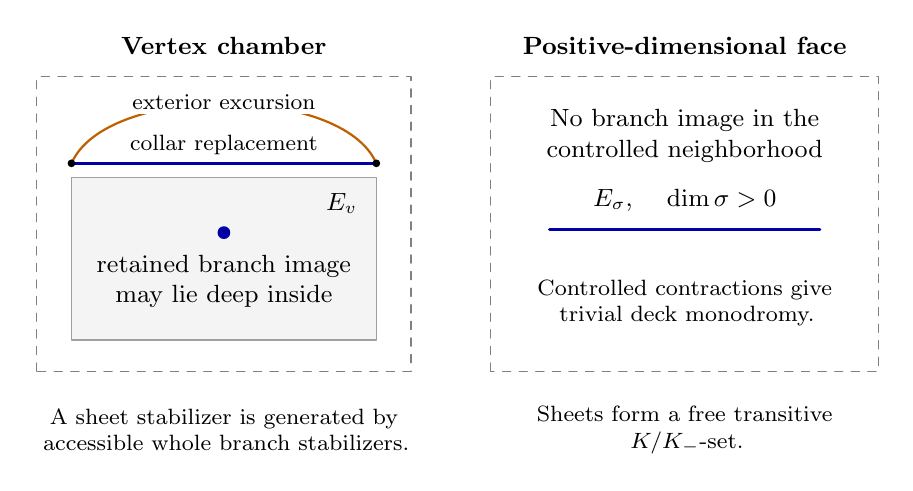
\begin{tikzpicture}[x=.88cm,y=.88cm,font=\small,
  every node/.style={align=center},line cap=round,line join=round]
  \node[font=\small\bfseries] at (2.8,5.35) {Vertex chamber};
  \draw[dashed,gray] (.1,.65) rectangle (5.5,4.9);
  \filldraw[fill=gray!9,draw=gray!75] (.6,1.1) rectangle (5,3.45);
  \node at (4.5,3.07) {$E_v$};
  \fill[blue!65!black] (2.8,2.65) circle (2.3pt);
  \node[text width=3.7cm] at (2.8,1.95)
    {retained branch image\\may lie deep inside};
  \draw[thick,orange!75!black]
    (.6,3.65) .. controls (1.1,4.8) and (4.5,4.8) .. (5,3.65);
  \node[font=\footnotesize,fill=white,inner sep=1.5pt] at (2.8,4.53)
    {exterior excursion};
  \draw[very thick,blue!65!black] (.6,3.65)--(5,3.65);
  \fill (.6,3.65) circle (1.4pt);
  \fill (5,3.65) circle (1.4pt);
  \node[font=\footnotesize,fill=white,inner sep=1pt] at (2.8,3.91)
    {collar replacement};
  \node[font=\footnotesize,text width=4.75cm] at (2.8,-.2)
    {A sheet stabilizer is generated by\\accessible whole branch stabilizers.};

  \node[font=\small\bfseries] at (9.45,5.35)
    {Positive-dimensional face};
  \draw[dashed,gray] (6.65,.65) rectangle (12.25,4.9);
  \node[text width=4.3cm] at (9.45,4.05)
    {No branch image in the\\controlled neighborhood};
  \draw[very thick,blue!65!black] (7.5,2.7)--(11.4,2.7);
  \node at (9.45,3.12) {$E_\sigma$, \quad $\dim\sigma>0$};
  \node[font=\footnotesize,text width=4.35cm] at (9.45,1.63)
    {Controlled contractions give\\trivial deck monodromy.};
  \node[font=\footnotesize,text width=4.85cm] at (9.45,-.2)
    {Sheets form a free transitive\\$K/K_-$-set.};
\end{tikzpicture}
\caption{Schematic coarse neighborhoods for selective cubulation. The
closed mid-halfspace chamber $E_v$ may contain retained branch images;
only the exterior collar used to shorten excursions must avoid them.
Every positive-dimensional face chamber $E_\sigma$ has a branch-free
controlled neighborhood. Consequently sheet transitions between
positive-dimensional faces are equivariant bijections, whereas vertex
sheet stabilizers may be nontrivial. The drawn regions and distances
are schematic: $E_v$ is not asserted to be the literal fiber
$p^{-1}(v)$, and the collar constants do not depend on chamber diameter.}
\label{fig:selective-chambers}
\end{figure}


Construct \(\widetilde Y\) by taking one copy of each cube of \(Y\) per
sheet of \(E_\sigma\), gluing along the face transitions.  These transitions
are compatible by construction, so this is a cubical complex, with
\begin{equation}
 q:\widetilde Y\longrightarrow Y
 \label{fill:cubical-cover}
\end{equation}
and an action of \(P\), inducing the \(\bar H\)-action downstairs.

\begin{lemma}[Cubical branched model]\label{fill:cubical}
The complex \(\widetilde Y\) is CAT(0), the \(P\)-action is cocompact,
and every hyperplane maps isomorphically under \(q\) to a hyperplane of
\(Y\).
\end{lemma}

\begin{proof}
First consider links.  Two adjacent lifted edge germs project to
distinct germs, since they occur on a cube projecting isomorphically
to a base cube.  Hence a clique projects to a clique with distinct germs.
An individual lifted edge determines a unique lift of every
positive-dimensional containing cube by the positive-face bijections
of Lemma~\ref{fill:sheets}.  The base flag condition and these bijections
therefore place all germs of the clique on its unique lifted cube.
Links are simplicial and flag.

We now establish simple connectivity; local flagness alone would not
suffice.  There is a useful canonical-lifting rule.  Suppose \(b\) maps
a path, disc, or homotopy into \(\widetilde X\), and \(a\) maps the same
parameter space into \(C\), with
\begin{equation}
 d\bigl(a,f\pi b\bigr)\le 2r+10r_0.
 \label{fill:close-maps}
\end{equation}
By the choice of \(D\), if \(p a\) lies in the open
cube \(\sigma\), the open-cube estimate in Lemma~\ref{fill:collapse}
assigns \(b\) to a sheet of \(E_\sigma\).  Use the corresponding copy of
\(\sigma\) to lift \(p a\).

This lift is continuous.  Near a parameter mapping into an open face,
local finiteness downstairs confines nearby values to cofaces of that
face.  Local path connectivity of the parameter space and the collar
assignment in Lemma~\ref{fill:sheets} make their sheet restrictions
agree on the face.  Although there can be infinitely many coface sheets
upstairs, their points approach this same face lift: distance to the
face is bounded by the corresponding coordinate distance inside a
unit cube, uniformly in dimension.  Thus the rule is continuous in
the cubical path metric.  In particular it applies to \(a=f\pi b\).

Conversely, let \(\alpha\) be an edge loop in \(\widetilde Y\), viewed
as a loop based at an edge midpoint.  For each of its edge occurrences
choose \(c_e\in E_e\) projecting to that midpoint, using the cube-lifting
assertion of Lemma~\ref{fill:collapse}.  Choose a nearby reference point
\(z_e\in\widetilde X\) in its assigned edge sheet.  Consecutive reference
points belong to the same vertex sheet, so join them by paths over the
\(r\)-neighborhood of the relevant \(E_v\).  These paths concatenate
to a loop \(b\) in \(\widetilde X\).

Project the image \(f\pi b\) piecewise to the convex sets \(E_v\),
adjusting its endpoints to the chosen \(c_e\)'s.  Nearest-point projection
and bounded endpoint interpolation give a homotopy satisfying
\eqref{fill:close-maps}.  Its canonical lift ends in paths lying in
closed half-stars of the prescribed lifted vertices.  To see this
precisely, a point of \(E_v\) has all outside-wall orientations equal
to those of \(v\), and every variable coordinate is at most halfway
from that corner.  Face consistency fixes the assigned lifted corner
throughout each path piece.  Straight-line contraction towards that
corner, compatible on faces, replaces the piece by the two required
half-edges.  The resulting loop is \(\alpha\).

Since \(\widetilde X\) is simply connected, \(b\) bounds a disc there.
The canonical lift for \(a=f\pi b\) maps this disc into
\(\widetilde Y\), proving that \(\alpha\) is nullhomotopic.
Every lifted vertex is also connected to the canonical image:
choose a reference point close to a lift of a base vertex in \(E_v\)
and use the same bounded interpolation.  Thus \(\widetilde Y\) is
connected and simply connected.  All cells have bounded finite shapes
and embedded faces; after subdivision, metric-open cell stars allow
ordinary fine-mesh simplicial approximation of the compact discs just
used.  Hence this argument proves the usual combinatorial simple
connectivity as well. Together with flag links it proves the CAT(0)
conclusion by \cite[Lecture~1, Section~1.2]{Sageev2014}.

The action is cocompact because \(Y/\bar H\) has finitely many cube
orbits and \(B\) is transitive on every sheet set.  Finally,
positive-dimensional face transitions make the restriction of \(q\)
to a hyperplane an ordinary covering of a base hyperplane.
Base hyperplanes are CAT(0), hence simply connected.  Each such
covering is therefore an isomorphism.
\end{proof}

\begin{proof}[Completion of Proposition~\ref{fill:selective}]
Take the finitely many hyperplane orbit families of the compact special
cover of \(C\), omitting families with no surviving members.  Within
each family hyperplanes are two-sided and disjoint.  These properties
pass to \(Y\): remaining walls do not acquire new crossings, by
Lemma~\ref{fill:collapse}.  They also pass to \(\widetilde Y\).

Cut successively along the lifts of each family, within the convex
components left by previous cuts.  Disjoint two-sided tracks in a
simply connected component give a tree splitting.  The resulting
graph-of-groups quotients are finite.  Indeed, subdivide along the
midplanes.  A chamber and its incident side pieces are specified by
cube-side flags up to the group action.  At a cell only the hyperplanes
cutting that cell can vary the choices of sides, so the number of
choices is bounded in terms of the dimension.  Branching at original
vertices introduces no additional midplane choices.

A cutting trace is a convex part of a lifted hyperplane.  It contains
a dual-edge midpoint in its chamber: in a cube meeting the trace, fix
the dual coordinate at its middle and choose the remaining corner
coordinates towards the chamber's defining sides.  Thus the trace
determines its containing hyperplane.  A deck transformation preserving
the trace preserves this hyperplane, acts trivially on it by
Lemma~\ref{fill:cubical}, and is trivial because positive-cell sheet
actions are free.  Hence the trace stabilizer injects into \(\bar H\).

The trace projects to a convex subcomplex of the corresponding base
hyperplane.  Each earlier cutting hyperplane meeting the lifted
hyperplane has a unique corresponding base trace; thus its side
condition projects to the same convex halfspace condition downstairs.
The stabilizer acts cocompactly on the trace by the finite flag
description.  Its image is consequently undistorted in \(Q_*\).
The quotient map \(P\to\bar H\) is Lipschitz in word metrics, so this
also proves undistortion of the trace stabilizer in the hyperbolic
group \(P\).  All edge groups of the hierarchy are therefore
quasiconvex in \(P\).

After all families are cut, each component has one original cubical
vertex.  Its stabilizer projects trivially to \(\bar H\), since
\(\bar H\) is torsion-free and acts properly on \(Y\).  It is exactly
the deck stabilizer of the corresponding vertex sheet.
Lemma~\ref{fill:sheets}(iii) says that this group is generated by
whole accessible retained factors, with finitely many factor orbits.
Apply Kurosh to its subgroup of
\[
 B=\mathop{*}_{a\ {\rm retained}}R_a.
\]
Each accessible whole factor is one of its Kurosh factors, up to
subgroup conjugacy.  Killing these factors kills the entire sheet
stabilizer by the proved generation statement.  Hence there can be
no remaining free summand or partial-factor summand.  The vertex
stabilizer is a finite free product of retained factors and is
hyperbolic and virtually compact special.

The hierarchy has finitely many levels and finite quotients.
Working upwards from its terminal groups shows that all vertex
groups are finitely generated.  The globally quasiconvex edge
groups give quasiconvex vertex groups successively: replace
excursions of an ambient path outside a vertex space by paths in
the attaching edge cosets, using their ambient undistortion.
The quasiconvex hierarchy theorem \cite{Wise2021} therefore makes
\(P\) virtually compact special.  The normal-core choice made above
establishes the asserted normality of \(H\), and any later normal
core can be accommodated by repeating the same sparse-cover
construction.
\end{proof}

\subsection{Novikov realization along quotient chains}

The geometric construction now supplies quotients that retain any
prescribed finite set of filling-kernel factors. Our algebraic target is
to realize any finite list of rational expressions, after finite-index
restriction, in the ordinary Novikov rings for both signs of one real
character. Applied to the entries of a division-ring chain contraction,
this will give the two acyclicity statements needed for fibering.
We first descend through an RFRS chain of the quotient until the
remaining coefficients lie in \(D(K)\). A selective quotient then
makes their finitely many subgroup supports detectable by a second
RFRS chain. That descent ends with ordinary group-ring coefficients;
recombination recovers the original expressions for one character and
its negative.

For a real character \(\chi:J\to\R\), write
\begin{equation}
 \widehat{\Q J}^{\,\chi}
 =\left\{\sum_{g\in J}a_g g:
       \#\{g:a_g\ne0,\ \chi(g)<c\}<\infty
       \text{ for every }c\in\R\right\}.
 \label{fill:novikov-ring}
\end{equation}
Our completion convention is towards positive height.
The subgroup-field hypotheses embed \(D(J)\) and this ring in the same
skew series division ring over \(D(\ker\chi)\).  Indeed,
\eqref{fill:field} embeds the rational field there; a nonzero series
has a leading term, and its positive remainder has a positive minimum
valuation, so geometric inversion is defined.  This remains valid when
\(\chi(J)\) is dense in \(\R\), because the support condition is finite
below each threshold.

\begin{definition}\label{fill:selective-input}
Let \(K\lhd J\), with \(J/K\) virtually RFRS.
We say that \((J,K)\) has the \emph{selective realization property} if,
for every finite-index preimage \(J'\le J\) and every finite set
\(T\subset K\), there are a finite-index preimage \(H\le J'\), normal
in \(J'\), a subgroup \(U\le K\) containing \(T\), and a homomorphism
from \(H\) to a virtually RFRS group that is injective on \(U\).
\end{definition}

Proposition~\ref{fill:selective} supplies this property in
Theorem~\ref{fill:criterion}: a finite set in \(K\) lies in a finite
subproduct of \eqref{fill:CL}, and its selective quotient is virtually
compact special, hence virtually RFRS \cite{Agol2008}.
More explicitly, let \(\rho:H\to L\) be the selective homomorphism
and let \(S\) be a finite transversal for \(H\backslash J'\).
Normality of \(H\) makes
\[
 h\longmapsto\bigl(\rho(s^{-1}hs)\bigr)_{s\in S}
 \qquad(h\in H)
\]
a homomorphism on the common domain \(H\). Its \(s\)-coordinate is
injective on \(sUs^{-1}\). These are the conjugate support groups
arising in the right-coset coordinates for restriction of scalars.
Finite products
and subgroups of RFRS groups are RFRS, so the product target remains
virtually RFRS.

\begin{lemma}[Controlled linearization]\label{fill:linearize}
A rational expression over a coefficient ring in a division ring has
a representation \(pA^{-1}q\), where \(A\) is a square polynomial
matrix and \(p,q\) are constant selectors.  The entries of \(A^{-1}\)
can be given rational expressions using sums and products of the
original subexpressions and their original inverses.  In particular
linearization introduces neither a larger nested inverse depth nor
new bottom denominators on a maximal-depth inverse chain.
\end{lemma}

\begin{proof}
A polynomial \(f\) is the upper-right entry of the inverse of
\(\begin{psmallmatrix}1&-f\\0&1\end{psmallmatrix}\).
Use block diagonals for sums.  If \(E=pA^{-1}q\) and \(F=rB^{-1}s\),
use
\[
 \begin{pmatrix}A&-qr\\0&B\end{pmatrix}^{-1}
 =
 \begin{pmatrix}
 A^{-1}&A^{-1}qrB^{-1}\\0&B^{-1}
 \end{pmatrix}
\]
for the product.  For \(E^{-1}\), border \(A\) to obtain
\begin{equation}
 M=\begin{pmatrix}0&p\\q&A\end{pmatrix},\qquad
 M^{-1}=
 \begin{pmatrix}
 -E^{-1}&E^{-1}pA^{-1}\\
 A^{-1}qE^{-1}&A^{-1}-A^{-1}qE^{-1}pA^{-1}
 \end{pmatrix}.
 \label{fill:border}
\end{equation}
The displayed formulas prove the assertion inductively.  In
\eqref{fill:border} the new inverse is exactly the parent inverse
already present in the original expression.
\end{proof}

The data at a descent stage are finitely many square polynomial
matrices invertible over the current division ring, together with
chosen rational expressions for all entries of their inverses.
Linearization puts a finite list of scalar expressions in this form.
Truncating a character expansion records finitely many coefficient
entries. Solving those coefficient problems means realizing their
chosen rational values in both ordinary Novikov rings for one later
character. The next lemma proves that this reduction terminates;
the following lemma explains how to recover the original inverses.

\begin{lemma}[Finite descent of inverse depth]\label{fill:ancestry}
Let \(J/K\) have a normal RFRS chain, and pull it back to
\[
 J=H_0\ge H_1\ge\cdots,\qquad \bigcap_iH_i=K.
\]
Let \(N_i\lhd H_0\) be the preimage of the rational abelianization
kernel of \(H_i/K\), so \(N_i\le H_{i+1}\).
At each stage expand finitely many specified rational expressions
for both signs of a character with kernel \(N_i\), retain finitely
many coefficients, restrict those scalar coefficient problems to
\(H_{i+1}\), and use Lemma~\ref{fill:linearize}.
After finitely many stages the resulting coefficient problems have
inverse depth zero over \(D(K)\).
\end{lemma}

\begin{proof}
Inverse depth is measured relative to \(D(K)\): coefficient-field
elements and group monomials have depth zero, sums and products
take the maximum, and inversion adds one.  At the bottom of an
inverse chain, evaluate the inverse-free operand as a finite
polynomial before taking slices.

For one character, write an operand with leading monomial \(L\) as
\(L(1+T)\), with \(T\) of strictly positive valuation.  Its inverse
is \(\sum_{n\ge0}(-T)^nL^{-1}\).  Every specified coefficient is a
finite sum of products of operand coefficients, monomial transports,
and the inverse of the leading coefficient.  Thus depth does not
increase.

There is a more precise invariant.  If a coefficient retains the
old maximum depth \(d>0\), each bottom denominator on a length-\(d\)
inverse chain is a height slice of an old bottom polynomial on a
length-\(d\) chain, up to common monomial transport and conjugation.
For sums and products the assertion follows by tracing a
maximal-depth chain into one factor.  For an inverse, coefficients
of its operand alone have depth at most \(d-1\).  A chain of length
\(d\) must therefore pass through the inverse of the leading
coefficient.  Apply the same induction to that coefficient of the
operand.  At the bottom this is simply a slice of an inverse-free
polynomial.  Cancellations remove terms but introduce no new support
degree in that bottom polynomial.

Choose one right normalizing monomial for each slice.  Replacing
support elements \(g,h\) by \(gu^{-1},hu^{-1}\) leaves \(gh^{-1}\)
unchanged.  A later whole conjugation conjugates this ratio.
Consequently, while depth \(d\) persists, the nonidentity differences
of its bottom support degrees modulo \(K\) lie among conjugates of
a fixed finite list, chosen at the beginning of this depth block.

Restriction to the next subgroup does not mix the coefficients:
for \(c\in D(N_i)\) and a representative \(t\) of
\(H_{i+1}\backslash H_i\),
\begin{equation}
 t c=(tct^{-1})t,\qquad tct^{-1}\in D(N_i)\subset D(H_{i+1}).
 \label{fill:diagonal}
\end{equation}
Thus the coefficient operator is diagonal by conjugation on these
coset coordinates.  Controlled linearization also preserves the
invariant by Lemma~\ref{fill:linearize}.

The bottom support differences at stage \(i\) belong to \(H_i/K\).
Since these subgroups are normal and have trivial intersection,
eventually they exclude every element of the fixed finite list and
all its conjugates.  Every bottom operand on a surviving maximal-depth
chain is then a monomial over \(D(K)\).  Inverting it uses only a
monomial inverse and a coefficient-field inverse, so all such chains
shorten.  Start a new finite list after this depth drop and repeat.
There are finitely many depth drops.

The qualification about maximal depth is essential to this argument.
New denominator supports can appear after the depth drops; the
construction expressly starts a fresh finite list at that point.
It never asserts that one support list controls all later depths.
\end{proof}

A given RFRS chain may be replaced by one normal in its initial group.
Indeed, intersect its finitely many conjugates at each stage; the
rational abelianization kernel of a subgroup maps into that kernel
in every containing conjugate.  The RFRS containment therefore
persists under these cores. In the finitely generated setting of
Proposition~\ref{fill:progressive}, characters with kernel exactly
\(N_i\) exist by embedding the finite-rank free abelian group
\(H_i/N_i\) in \(\R\). A zero character is permitted at a stationary
stage. Depth zero over \(D(K)\) still allows coefficients in that
division ring: it need not mean a polynomial over \(\Q K\). Removing
precisely those remaining coefficients will require the selective
realization property.

\begin{lemma}[Recombination by perturbation]\label{fill:recombine}
Suppose a finite stage of the preceding procedure used a character
\(\chi_i\) on \(H_i\). For each of its polynomial matrices \(A\), fix
finite homogeneous truncations \(B_+,B_-\) of \(A^{-1}\) such that
\(I-AB_\pm\) and \(I-B_\pm A\) have strictly positive weights for
\(\pm\chi_i\), respectively. Suppose all scalar coefficients of the
matrices \(A,B_+,B_-\) have been realized, after restriction to a
finite-index subgroup \(F\), in both ordinary Novikov rings for a
character \(\psi\) of \(F\), compatibly with their rational-field values.
Then its original matrix inverse problems are realized for both
signs of
\begin{equation}
 \chi_i|_F+\epsilon\psi
 \label{fill:perturb}
\end{equation}
for every sufficiently small positive \(\epsilon\).
\end{lemma}

\begin{proof}
Let \(A\) be one polynomial matrix and \(B=A^{-1}\), with its
specified rational expressions. The chosen truncations \(B_+\) and
\(B_-\) have coefficients in \(D(N_i)\), and both errors
\begin{equation}
 I-AB_\pm,\qquad I-B_\pm A
 \label{fill:errors}
\end{equation}
have strictly positive weights in their respective directions.

First we check the support needed to compare the two characters.
This is necessary even when a later finite-index cut does not
contain \(N_i\).
For right-coset coordinates \(t_j\) of \(F\backslash H_i\), the
entry from \(t_j\) to \(t_k\) of a homogeneous term of degree \(u\)
is supported in the single height
\begin{equation}
 u+\chi_i(t_j)-\chi_i(t_k).
 \label{fill:offset}
\end{equation}
Its coefficient lies in one coset of \(D(F\cap N_i)\): use the
finite-index field decomposition on the intersection of its original
homogeneous coset with the selected matrix coset. Put \(U=F\cap N_i\)
and first remove this common monomial shift. Choose a finitely generated
subgroup of \(U\) supporting a rational expression for the remaining
coefficient, and expand there for the restriction of \(\psi\).
Uniqueness of rational inverses in the ambient skew-series ring
identifies this intrinsic expansion with the ambient one. At each
\(\psi\)-height an ordinary Novikov realization has only finitely many
group terms. Subgroup-coset independence applied to that finite
coefficient sum excludes terms outside \(U\). Multiplying back by the
common shift proves preservation of the original homogeneous support.
The same argument applies across the selective change of quotient,
where the support subgroup embeds.

On \(F\cap N_i\), the new character in \eqref{fill:perturb} is
\(\epsilon\psi\).  The internal series expansion is therefore
unchanged, with only its grading scaled; it represents the same
rational entry.  Every finite old-height slice remains summable.
For each sign, subtract the row-minus-column offsets in
\eqref{fill:offset} when measuring an error entry.
There are finitely many positive old-height slices, and their
\(\pm\psi\)-valuations are bounded below.  A common sufficiently
small positive \(\epsilon\) therefore keeps all adjusted error
valuations strictly positive.

Offsets telescope in matrix products.  Hence powers of either
error in \eqref{fill:errors} have valuations tending to positive
infinity, even in the unadjusted coordinates.  Geometric inversion
provides both a left and a right inverse for \(A\) in the relevant
ordinary Novikov ring; they coincide.  All identities are exact
because the rational field and the ordinary series were embedded
in the same skew series division ring.  The same choice of
\(\epsilon\) works for the finite lists for both signs.
\end{proof}

\begin{proposition}[Progressive characters]\label{fill:progressive}
Let \(J\) be finitely generated with the subgroup-field hypotheses,
and let \(K\lhd J\) satisfy the selective realization property of
Definition~\ref{fill:selective-input}.
Every finite family of rational expressions over \(\Q J\) can,
after restriction of scalars to a finite-index subgroup \(F\),
be realized compatibly in the ordinary Novikov rings for both signs
of a single real character of \(F\).

In particular, if a finite complex of finitely generated free
\(\Q J\)-modules is acyclic over \(D(J)\), then its restriction is
acyclic over both these Novikov rings.  If its degree-zero ordinary
homology is nonzero, the character is nonzero.
\end{proposition}

\begin{proof}
Take the preimage \(H_0\) of a finite-index RFRS subgroup of \(J/K\).
Restriction of scalars is right multiplication on right-coset
coordinates, using a normal core when necessary.  The finite-index
field decomposition makes this an exact finite matrix operation.
Linearize the finitely many expressions as in
Lemma~\ref{fill:linearize}, retaining the specified expressions for
all needed inverse entries.

Pull back a normal RFRS chain from \(H_0/K\).  At stage \(i\), use
\eqref{fill:field} to expand each inverse matrix for both signs of
a character \(\chi_i\) with kernel \(N_i\).  Truncate sufficiently
far to obtain the positive errors \eqref{fill:errors}.  Collect
the finitely many coefficients of the matrix and its truncations;
they lie in \(D(N_i)\).  Restrict to the next group by
\eqref{fill:diagonal}, and linearize these scalar problems.
Lemma~\ref{fill:ancestry} terminates this procedure with finitely
many unresolved coefficients in \(D(K)\).

Choose a finite set of elements of \(K\) supporting rational
expressions for all those coefficients.  Apply the selective
realization property, including its finite product of conjugate
maps, to obtain a normal finite-index preimage \(H\) and a map
injective on the required support subgroups.  Pass to the
preimage \(H_p\) of an RFRS subgroup of its image.

This cut can mix coefficient entries, so we describe it explicitly.
For a scalar \(c\in D(U_0)\), group the cosets of \(H_p\) into
orbits of right multiplication by \(U_0\).  An orbit has
representatives \(gu_j\), with \(u_j\in U_0\).
The entries of right multiplication by \(c\) in these coordinates
come from decomposing \(u_jc\) over
\[
 D(U_0\cap g^{-1}H_p g)
\]
and then conjugating by \(g\).  They therefore admit finite rational
expressions entirely in these subgroup fields.
Changing to one common transversal only multiplies entries by
monomials, which does not affect summability.

Start the depth argument afresh with these new expressions.
Use an RFRS chain in the new quotient and ordinary rational group
polynomials.  Work separately inside each support subgroup,
choosing its own monomial transporters when taking a height
coefficient.  Later coefficients remain in conjugates of that
support subgroup.  Once a coefficient lies in the current
character kernel, restriction to the next stage only conjugates
it, because that whole kernel is contained in the next subgroup.
Thus the maximal-depth ancestry argument applies exactly as
before.  The new quotient map is injective on each support subgroup,
so its normal RFRS chain separates the finite nonidentity support
lists.  This time the terminal problems are ordinary group-ring
polynomials, with no unresolved division-field coefficients.
They are realized for the zero character if necessary.

Now reconstruct the inverse problems backwards, through both
finite chains and the selective switch, using
Lemma~\ref{fill:recombine}.  At each step use both signs' residual
lists and choose one sufficiently small positive perturbation.
The result is a single character on a common finite-index subgroup
and compatible realizations of all original expressions for both
of its signs.

For the chain-complex assertion, include the entries of a
\(D(J)\)-chain contraction and all the inverse operands used in
their expressions.  Their exact identities persist under the
common series embeddings, giving contractions over the two
ordinary Novikov rings. Restriction of scalars does not change the
underlying chain complex or its ordinary homology. If the final
character were zero, its Novikov rings would be \(\Q F\), so these
contractions would contradict the assumed nonzero ordinary
degree-zero homology.
\end{proof}

\begin{corollary}[Open Novikov regions for RFRS groups]\label{fill:rfrs-novikov}
Let \(J\) be virtually RFRS with the subgroup-field hypotheses.
A finite family of bounded complexes of finitely generated free
\(\Q J\)-modules, with polynomial differential matrices and acyclic
extension to \(D(J)\), admits simultaneous ordinary Novikov contractions,
after passage to a finite-index subgroup \(F\), on a nonempty
antipodally invariant open subset of \(\Hom(F,\R)\).
Here the character space has the topology of pointwise convergence.
This property can be imposed after any prescribed further finite-index
restriction.
\end{corollary}

\begin{proof}
We use the descent above with \(K=1\), so there is no selective
switch. For finitely generated \(J\), the underlying realization is
also supplied by \cite[Theorem~5.2]{Kielak2020}. To retain the present
group generality, we first justify the ambient characters and the
character-field expansion without finite generation.

Choose a finite-index RFRS subgroup \(H_0\) and a normal residual
chain \((H_i)\). The embedding
\(H_0\hookrightarrow\prod_i H_0/H_i\) into a countable product of
finite groups gives \(|H_0|\leq|\R|\). If \(N_i\) is the rational
abelianization kernel of \(H_i\), the rational hull of the torsion-free
abelian group \(H_i/N_i\) therefore has dimension at most
\(\dim_{\Q}\R\). A rational-linear injection into \(\R\) supplies
a character of the whole group \(H_i\) with kernel exactly \(N_i\).
The quotient need not be free abelian or finitely generated. The
RFRS containment \(N_i\leq H_{i+1}\) still holds.

For any real character \(\chi\) of a subgroup \(H\), put
\(N=\ker\chi\). Coset independence embeds
\(D(N)*(H/N)\) in \(D(H)\). This crossed product is the directed
union of its subrings over finitely generated subgroups of \(H/N\).
Each such subgroup is free abelian of finite rank, and its crossed
product is an iterated skew Laurent Ore domain. Every pair of
elements lies in one such subring, where its left and right Ore
equations can be solved. The union is therefore Ore as well.
Its fraction division ring embeds in \(D(H)\), since \(D(N)\), the
group lifts and all inverses of nonzero elements lie there. Conversely,
the fraction ring contains \(\Q H\), so it contains its division
closure \(D(H)\). The fraction ring is thus exactly \(D(H)\),
proving \eqref{fill:field} in this generality.

The same skew-series realization applies: a nonempty support finite
below every real threshold has a least term, and each strictly positive
remainder has an individual positive minimum valuation. These facts
justify geometric inversion even when the character image is dense
or not finitely generated.

Start with the finitely many entries of division-ring chain
contractions. The descent in Lemma~\ref{fill:ancestry} uses only finite
rational expressions, finite retained coefficient lists and finite-index
transversals. Normal residuality removes its finite support-difference
lists, so it terminates with coefficients over \(D(1)=\Q\).
Lemma~\ref{fill:recombine} then applies backwards: there are finitely
many old-height slices and lower bounds for their later-character
valuations, so one positive perturbation works for both signs at each
stage. This gives simultaneous ordinary Novikov contractions.

For openness, linearize the finitely many contraction entries over
the ordinary group ring and truncate their realized inverse matrices
to finite group-ring matrices. The left and right inverse errors have
finitely supported strictly positive valuations. Their finitely many
strict evaluation inequalities define an open neighborhood in the
pointwise topology, and geometric inversion supplies the contractions
throughout it. Intersect the neighborhood for the positive sign with
the negative of the neighborhood for the negative sign, and then take
the union with its negative. This is the required nonempty antipodally
invariant open set.

On restriction to any deeper finite-index subgroup, a Novikov
series remains summable in its finite coset coordinates, with
only fixed monomial offsets.  Repeat the finite truncation
argument there to obtain openness in the larger character space.
\end{proof}

\subsection{From two-sided Novikov acyclicity to a free kernel}

\begin{lemma}[The degree-one Novikov implication]\label{fill:bns}
Let \(J\) be finitely presented, and let \(\chi:J\to\R\) be nonzero.
If degree-one homology vanishes over
\(\widehat{\Q J}^{\,\chi}\), then \(\chi\) belongs to the Bieri--Neumann--Strebel (BNS)
invariant.  If the vanishing holds for both signs, some nonzero
rational character has finitely generated kernel.
\end{lemma}

\begin{proof}
We include the rational-coefficient argument in the positive-completion
convention of \cite[Theorem~3.11]{Kielak2020}; Sikorav established the
integral-coefficient criterion \cite{Sikorav1987}.
Choose a symmetric generating set containing a generator \(t\)
with \(\chi(t)>0\).  In the positive completion the formal ray
\[
 c=\sum_{j\ge0}[t^j,t^{j+1}]
\]
has boundary \(-[1]\).  For each oriented generator \(x\), the
chain
\[
 [1,x]+xc-c
\]
is a cycle, hence bounds a completed rational two-chain in the
finite presentation complex.

Truncate that two-chain sufficiently high.  Since relators have
bounded height offsets, its boundary cancels every low term of
the displayed cycle.  Truncate both rays at a common sufficiently
large exponent \(k\).  The resulting finite one-chain can be
made to have arbitrarily high support and boundary
\[
 [xt^k]-[t^k].
\]
The component of its edge support containing one endpoint must
contain the other: the total boundary coefficient in a finite
connected component is zero.  Thus \(t^k\) and \(xt^k\) are joined
by an actual path at uniformly high height, for every generator
\(x\).

Translate these finitely many paths to replace each edge
\(g\to gx\) by a path from \(gt^k\) to \(gxt^k\).
Choose the height threshold so this replacement raises the
minimum height by a fixed positive amount.  Iterating pushes
any finite path above height zero.  Its original nonnegative
endpoints are connected to their pushed copies by positive
\(t\)-rays, so the nonnegative Cayley graph is connected.
This is the BNS condition.

The finite paths and their strict height inequalities persist
in a neighborhood of \(\chi\).  Applying the same construction
to \(-\chi\) gives both BNS conditions on a nearby nonzero
rational line.  The two-sided BNS criterion
\cite[Theorem~B1]{BNS1987}, also stated in
\cite[Theorem~3.10]{Kielak2020}, says that the kernel of its integral representative
is finitely generated.
\end{proof}

\begin{lemma}[A finitely presented kernel in dimension two]\label{fill:free-kernel}
Suppose \(\cd J\le2\) and \(J\) maps onto \(\Z\) with finitely
presented kernel \(M\).  Then \(M\) is free.
\end{lemma}

\begin{proof}
We have \(\cd M\le2\).  If \(\cd M=2\), finite presentation gives
a finite-length resolution of \(\Z\) by finitely generated
projective \(\Z M\)-modules, with the last module in degree two.
Its dual has nonzero degree-two cohomology:
otherwise its last map would split, and dualizing back would
shorten the original projective resolution.  Thus
\[
 H^2(M;\Z M)\ne0.
\]

As an \(M\)-module, \(\Z J\) is a direct sum of copies of \(\Z M\)
indexed by \(J/M=\Z\).  Finite generation of the resolution gives
the corresponding direct-sum description of \(H^2(M;\Z J)\).
The generator of \(J/M\) shifts the summands, with its conjugation
twist.  Its coinvariants are therefore nonzero.  The
Lyndon--Hochschild--Serre cohomology spectral sequence has only columns
zero and one for this quotient, so
\[
 H^3(J;\Z J)
 \cong H^1\bigl(\Z;H^2(M;\Z J)\bigr)\ne0,
\]
contrary to \(\cd J\le2\); see \cite{Brown1982,Bieri1976}.
It follows that \(\cd M\le1\), and Stallings--Swan
\cite{Stallings1968,Swan1969} makes \(M\) free.
\end{proof}

\begin{proof}[Proof of Theorem~\ref{fill:criterion}]
First suppose \(G_*\) is already VCS, as happens when the peripheral
family is empty after discarding trivial members or contains \(G_*\)
itself. Then \(G_*\) is virtually RFRS, so
Corollary~\ref{fill:rfrs-novikov} applies directly to its finite
classifying-space chains. This gives two-sided Novikov contractions
on a finite-index subgroup \(F\), without using the filling construction.

In the remaining case choose the cofinite good filling
\eqref{fill:cofinite}. Proposition~\ref{fill:selective} gives the
selective realization property, and Proposition~\ref{fill:progressive}
applied to the same chains again supplies two-sided Novikov
contractions on a finite-index subgroup \(F\).

In either case the restricted group-ring chain complex has
\(H_0\cong\Q\): it is the cellular complex of the same connected
universal cover, now with the \(F\)-action. The character cannot be
zero, since its Novikov ring would then be \(\Q F\), and a contraction
would contradict this ordinary \(H_0\). Lemma~\ref{fill:bns} therefore
gives a nonzero rational character on \(F\) with finitely generated
kernel. Rescaling its image gives an epimorphism \(F\to\Z\).

Coherence makes this kernel finitely presented.
Lemma~\ref{fill:free-kernel} makes it free, and finite generation
makes its rank finite.  The extension splits by choosing a lift
of a generator of \(\Z\), so the subgroup is finite-rank
free-by-cyclic.  It is hyperbolic, hence admits a proper cocompact
cubulation by \cite{HagenWise2016}; the elementary rank-zero case
is immediate.  Agol's theorem \cite{Agol2013} now gives virtual
compact specialness, which passes to the finite-index overgroup
\(G_*\).
\end{proof}

\section{Hyperbolic ascending tori}\label{sec:02-ascending}

For an injective endomorphism $\phi:F\to F$, write
\[
 J_\phi=\langle F,t\mid t^{-1}gt=\phi(g)\ (g\in F)\rangle.
\]
Its height homomorphism sends $t$ to $1$ and $F$ to $0$.
Changing the sign of height, or replacing the stable letter by its inverse,
will not affect any assertion below. A \emph{free splitting tree} means a
minimal simplicial tree with trivial edge stabilizers and finite quotient;
its vertex stabilizers are free factors. A path map of trees is
\emph{alignment preserving} if it maps each segment monotonically onto a
segment, allowing constant subsegments.

\begin{theorem}\label{asc:vcs}
Let $F$ be a free group of finite rank and let $\phi:F\to F$ be injective.
If $J_\phi$ is word-hyperbolic, then $J_\phi$ is virtually compact special.
\end{theorem}

We prove the theorem by induction on $\rk F$. The rank-zero group is
infinite cyclic. Rank one gives $\mathrm{BS}(1,n)$, with $n\ne0$, and is
incompatible with hyperbolicity. When $\phi$ is an automorphism, the
conclusion follows from the cubulation theorem for hyperbolic
free-by-cyclic groups \cite{HagenWise2016} and Agol's theorem
\cite{Agol2013}. For a nonsurjective injection, we either reduce rank or
construct a noncontracting map of a free splitting tree. In the expanding
case, its associated real-tree action gives a finite family of point
stabilizers with nontrivial height-zero part. They are virtually
ascending tori of smaller rank and will serve as peripherals.
Filling their height-zero parts makes the base virtually free; a finite
graph cover then separates the expanding map into irreducible train-track
blocks. We remove any failure of fundamental-group injectivity in those
blocks before applying Hagen--Wise. This supplies the good fillings for
Theorem~\ref{fill:criterion}. The nonexpanding case is handled directly
by a quasiconvex hierarchy.

The ascending result is also an input to the filling construction in
Section~\ref{sec:06-closure}. After proving it, we recover its stronger
virtual finite-rank free-by-$\Z$ consequence in
Corollary~\ref{cor:ascending-finite-rank}, including the induction branches
that do not directly use the filling criterion.

\subsection{Finiteness hypotheses and elementary changes of model}

\begin{lemma}\label{asc:field-hypotheses}
An ascending torus of an injective finite-rank free-group endomorphism is
torsion-free, locally indicable, coherent, residually finite, and has a
finite aspherical complex of dimension at most two. It has the
Hughes-free subgroup-field setup used in Theorem~\ref{fill:criterion}, and
its finite cellular chain complex becomes acyclic over its rational
Linnell field.
\end{lemma}

\begin{proof}
The height kernel is an increasing union of conjugates of $F$.
Consequently a finitely generated subgroup contained in that kernel lies
in a free group and, if nontrivial, maps onto $\Z$. A subgroup not contained
in the kernel has a nonzero height homomorphism. This proves local
indicability and also torsion-freeness. Coherence is the theorem of
Feighn--Handel, which includes injective endomorphisms
\cite[Theorem~1.1]{FeighnHandel1999}. Residual finiteness is due to Borisov--Sapir
\cite{BorisovSapir2005}.

Represent $\phi$ by a based map of a finite rose. Its mapping torus is a
finite aspherical two-complex: the associated graph of spaces has
contractible vertex and edge universal covers and injective attaching
homomorphisms. The usual tree-of-spaces construction therefore gives a
contractible universal cover.

The height kernel belongs to Linnell's class generated by free groups
under directed unions; its extension by $\Z$ belongs to the same class
under elementary-amenable extensions. Linnell's theorem, together with
the locally indicable Hughes-free field setup, gives the rational
subgroup fields, their compatible inclusions and coset independence
\cite{Linnell1993,Hughes1970}; the locally indicable affiliated realization
and compatible rational subfields are given by
\cite[Corollaries~6.2--6.3]{JaikinLopezAlvarez2020} and
\cite[Section~2.3 and Proposition~2.2]{JaikinUniversality2021}.
In particular the field embeds in the
height skew-series division ring with coefficients in the kernel field,
with either order on height.

For completeness, take a basis $x_1,\ldots,x_r$ of $F$ and the relators
$t^{-1}x_it\phi(x_i)^{-1}$. The horizontal Fox matrix is
\[
 M=t^{-1}I-\left(\frac{\partial\phi(x_i)}{\partial x_j}\right)_{i,j}.
\]
After removing the invertible initial factor $t^{-1}$, its initial
height term is $I$. Geometric-series inversion therefore makes $M$
invertible in a height skew-series division ring. A square matrix over a
division subring that is invertible over an extension division ring is
already invertible over the subring, so $M$ is invertible over the
Linnell field. Thus the second boundary is injective after base change.
The zeroth homology vanishes because $t-1$ is invertible in that field.
The cellular Euler characteristic is $1-(r+1)+r=0$, so the first homology
vanishes as well.
\end{proof}

We will use the following elementary observation twice. It applies even
when a graph map is not injective on fundamental groups.

\begin{lemma}\label{asc:shift-equivalence}
Suppose based maps $f:X\to X$ and $g:Y\to Y$ of connected finite graphs
admit based maps $q:X\to Y$ and $i:Y\to X$ such that
\[
 qf=gq,\qquad ig=fi,\qquad iq=f^m,\qquad qi=g^m
\]
for some $m\ge1$. Their mapping-torus groups are isomorphic, by an
isomorphism preserving height.
\end{lemma}

\begin{proof}
The commuting maps induce homomorphisms of the mapping-torus
presentations, sending stable letter to stable letter. Their composites
are induced by $f^m$ and $g^m$. In a mapping-torus presentation the map
induced by the defining endomorphism is conjugation by the stable letter;
hence both composites are inner automorphisms. The two homomorphisms are
therefore isomorphisms. The same argument works up to based homotopy,
with the corresponding change of stable-letter marking.
\end{proof}

\subsection{An expanding relative tree model}

Expanding relative immersions for injective, nonsurjective free-group
endomorphisms
were constructed by Mutanguha
\cite[Proposition~4.1 and Theorem~4.5]{Mutanguha2021Dynamics}.
The following form is tailored to the induction on rank.

\begin{lemma}\label{asc:relative-model}
Let $\phi:F\to F$ be injective and nonsurjective, with $\rk F\ge2$.
After replacing $F$ by an iterated image, one of the following holds.
\begin{enumerate}[label=\textup{(\roman*)}]
\item A finite-index height subgroup of $J_\phi$ is an ascending torus of
an injection of a free group of rank strictly smaller than $\rk F$.
\item There is a nontrivial free splitting tree $T$ and a
$\phi$-equivariant embedding $f:T\to T$ that is a homothety of scale
$\lambda\ge1$. The edge-transition matrix is irreducible, every vertex
stabilizer is a proper free factor, and the quotient graph is finite.
\end{enumerate}
\end{lemma}

\begin{proof}
We compare successive iterated-image core graphs using the lengths of
their arcs between branch vertices. Collapsing the arcs whose lengths
stay bounded gives two trees and two maps: substitution identifies the
collapsed trees, while their original inclusion gives a possibly
collapsing map back. Their composition yields the required self-map.
Its transition diagram will either lose an edge orbit, allowing rank
reduction, or supply a recurrent irreducible part.

Fix the unit-edge Cayley tree $S$ of $F$. Put $F_n=\phi^n(F)$ and let
$S_n\subset S$ be its convex minimal subtree. Each $S_n$ is leafless.
Suppress the vertices of valence two and call the resulting edges
\emph{natural arcs}. The finite core graph $F_n\backslash S_n$ has rank
$r=\rk F$, and thus at most $3r-3$ natural edges.

Substitution by the fixed injection $\phi$ is a quasi-isometric embedding
of $S$: its image group is finitely generated and undistorted in $F$.
Restricting to $S_n$ and straightening to the hull $S_{n+1}$ gives
$\phi$-equivariant quasi-isometries
\[
 S_n\longrightarrow S_{n+1}
\]
with constants independent of $n$. Indeed the boundary of the target
hull is the image of the source boundary, and straightened axes remain
within the uniform quasigeodesic-stability bound. Branch points are
centers of tripods with three unbounded legs. These quasi-isometries
therefore give uniformly controlled branch-point correspondences in
both directions; the two composites move branch points a uniformly
bounded distance.

Choose a subsequence of pairs
\[
 U_k=S_{n_k},\qquad V_k=S_{n_k+1}
\]
on which the two finite reduced core-graph types are fixed and each of
their natural-edge lengths is either bounded or tends to infinity.
There is one bound $B$ for all bounded coordinates, and the minimum
$\ell_k$ of all unbounded coordinates tends to infinity. Collapse in
$U_k$ and $V_k$ the components of their respective bounded-arc forests.
These forests need not have bounded-diameter components.

For sufficiently large $k$, the branch-point correspondence induces a
$\phi$-equivariant simplicial isomorphism between the two collapsed
trees. Here are the details needed when a collapsed component is
unbounded. Adjacent branch points joined by a bounded arc have images
at a uniformly bounded distance. Their images consequently lie in the
same bounded-arc component, since that distance is less than $\ell_k$.
Apply this to chains of bounded arcs and then apply the coarse inverse;
the bounded errors of the two composites show that the resulting maps
on components are inverse bijections. To verify adjacency, let $[v,w]$
be a long natural source arc and choose the corresponding target branch
points $v',w'$. For every branch point $z$ of $[v',w']$, quasigeodesic
stability puts its corresponding source branch point within a uniform
distance of $[v,w]$. The projection of a branch point to the interior of
a branch-free natural arc is impossible: an off-arc branch point would
create a branch point where its joining arc meets the interior. Its
projection is therefore $v$ or $w$. It follows that $z$ is uniformly
close to $v'$ or $w'$. If $[v',w']$ crossed two long target arcs, a branch
point between them would be at distance at least $\ell_k$ from both
endpoints, a contradiction. It crosses at least one long arc because
the endpoint short components are distinct. Thus it crosses exactly
one. The reverse correspondence gives the same conclusion in the
opposite direction, proving adjacency.

The collapsed tree is nontrivial for some such subsequence. Otherwise
all natural arcs have uniformly bounded lengths along an infinite
subsequence. There would then be only finitely many unbased labelled
core graphs, so two nested groups $F_n,F_{n+j}$ would be conjugate. A
finitely generated subgroup of a free group cannot be conjugate to a
proper subgroup of itself. To see this last fact directly, if
$gAg^{-1}\le A$, the nested translates $g^{-i}S_A$ all contain $S_A$.
Fix a point on an axis in $S_A$. Since $A$ acts cocompactly on $S_A$,
that point is a uniformly bounded distance from every coset $g^{-i}A$.
Only finitely many cosets can meet a fixed finite ball, so $g^j\in A$
for some $j>0$. The nested conjugacy chain is now periodic and all its
inclusions are equalities. Hence $F_n=F_{n+j}$, which by injectivity
implies $F=\phi^j(F)$ and contradicts nonsurjectivity.

Inclusion $V_k\subset U_k$ maps bounded-arc components to bounded-arc
components. In fact a bounded natural arc of $V_k$ is subdivided by
branch points of $U_k$ into arcs of length at most $B<\ell_k$.
Fix one sufficiently large $k$, and write $n=n_k$ and
$T_U,T_V$ for the collapsed trees. Their actions are the actual actions
of $F_n$ and $F_{n+1}$, respectively. The maps just constructed are
\[
 T_U\xrightarrow{\ \Phi_k\ }T_V
     \xrightarrow{\ I_k\ }T_U.
\]
Here $\Phi_k$ is a simplicial isomorphism equivariant for
$\phi:F_n\xrightarrow{\sim}F_{n+1}$, and $I_k$ is alignment preserving
and equivariant for the inclusion $F_{n+1}\leq F_n$. Hence
$I_k\Phi_k$ is a $\phi$-equivariant alignment-preserving self-map of the
single $F_n$-tree $T_U$. The subsequence was used to classify natural-arc
lengths; no identification of the markings at different $k$ is needed.
Replacing the base by $F_n$
does not change the ascending torus: the base $F$ is conjugate into
$F_n$ by a power of the stable letter, and ascending normal form
gives the converse inclusion. Rename this base $F$.

If an iterate of the whole tree misses an edge orbit, its connected
image lies in one component of the complement of that orbit. The image
group $\phi^m(F)$ stabilizes that component. Its stabilizer $C$ is a
proper free factor, as follows by collapsing every complementary
component in the original free splitting. Consequently
\[
 \phi^m(F)\le C,\qquad \phi^m(C)\le C.
\]
The ascending torus of $\phi^m|_C$ embeds by normal form in the height-$m$
subgroup, and contains its whole base after conjugating by the stable
letter. It is therefore that subgroup. This is alternative (i).

Otherwise choose a source strongly connected component in the finite
edge-transition diagram. If it were nonrecurrent, it would consist of
one vertex with no self-loop and no incoming arrow; that edge orbit
would already be missing from the image of the whole tree. The chosen
component is therefore recurrent. No incoming arrows means that each
edge outside it maps entirely through edges outside it. Their union is
an invariant forest in the tree, so collapsing it gives a well-defined
self-map. Each remaining edge has a transition inside the recurrent
component and is not collapsed. Alignment preservation also survives:
lift a segment through
the collapsed vertex components, apply alignment preservation before
collapse, and delete the collapsed subsegments. No reduced path can
acquire backtracking in this operation. The transition matrix is now
irreducible. Its Perron eigenvector assigns positive lengths to the
finitely many edge types, and linear parametrization makes the map
multiply all path lengths by the Perron eigenvalue $\lambda\ge1$.
Alignment preservation and noncollapse make it an embedding.
All vertex stabilizers are proper free factors because the resulting
free splitting is nontrivial. This proves alternative (ii).
\end{proof}

\subsection{Point stabilizers and their quasiconvexity}

Assume alternative (ii) of Lemma~\ref{asc:relative-model}. Over each
vertex $b$ of the ascending Bass--Serre tree $\mathcal B$ place a copy
$T_b$ of $T$. Orient $\mathcal B$ toward its distinguished end, so every
vertex has one parent and any two upward rays eventually agree. The
attaching map to the parent is the homothety $f$. Rescale the metric in
each copy according to its height so that these maps are isometric
embeddings. Their convex directed union is a real tree $\mathcal T$;
it need not be complete. The torus acts on it by homotheties, whose
scales are powers of $\lambda$ determined by height.

\begin{lemma}\label{asc:point-stabilizers}
The height-zero subgroup of $J_\phi$ has trivial stabilizers of
nondegenerate arcs of $\mathcal T$. There are finitely many
$J_\phi$-orbits of points with nontrivial height-zero stabilizer.
For each such point $x$, the full stabilizer $A_x$ has a finite-index
subgroup that is an ascending torus on a proper free factor of $F$.
If $\lambda>1$, the family of these point stabilizers is malnormal.
\end{lemma}

\begin{proof}
For a height-zero element and a compact arc, choose a sufficiently high
ancestor copy containing both endpoints and whose base group contains
the element. A nontrivial element fixing that arc would fix an edge of
the free splitting, which is impossible.

Suppose a nontrivial base element fixes $x$. Its own copy $T_b$ is a
complete simplicial tree, since its finitely many edge lengths have a
positive minimum. It is thus a closed convex subtree of $\mathcal T$.
If $x$ were outside it, the element would fix the segment from $x$ to
its nearest point in $T_b$, contradicting the preceding paragraph.
Hence $x\in T_b$ and is a vertex with nontrivial vertex stabilizer.

Let $C_{b,x}$ be the stabilizer of $x$ in the base group at $b$, and
consider the vertices $b$ for which $C_{b,x}\ne1$. They form a connected
parent-closed subtree of $\mathcal B$: nontrivial elements remain
nontrivial on passing to a parent, and upward rays coalesce. There are
only finitely many types of pairs $(b,x)$ modulo $J_\phi$, because the
free splitting has finite quotient. This proves finiteness of point
orbits. On an upward ray two pair types repeat, yielding an element
$s\in A_x$ of positive height that takes one vertex $b$ to an ancestor.
Its positive translates are cofinal along that ray. Every height-zero
element of $A_x$ belongs to a sufficiently high base group and fixes
$x$ there. Consequently $\ker(h|_{A_x})$ is the increasing union of the
corresponding translates of $C_{b,x}$. The subgroup with heights in
$h(s)\Z$ is therefore the ascending torus based on $C_{b,x}$, with stable
letter $s$ and the appropriate orientation. It has finite index in
$A_x$. The group $C_{b,x}$ is a proper free factor, so has smaller rank.

Finally suppose $\lambda>1$. An element fixing two distinct points has
scale one, hence height zero. It must then be trivial by the arc
assertion. Thus distinct point stabilizers intersect trivially, including
conjugate stabilizers of distinct points. This is precisely malnormality
for a list of orbit representatives.
\end{proof}

If $\lambda=1$, irreducibility and Perron eigenvalue one imply that the
transition matrix is a cyclic permutation matrix. The maps take edges
to single edges. The union tree is simplicial and its torus quotient is
finite. Its edge stabilizers inject into the height group and are
therefore cyclic or trivial. Vertex stabilizers either inject into
height or are those in Lemma~\ref{asc:point-stabilizers}. Cyclic edge
groups are quasiconvex in the hyperbolic torus. The vertex groups are
finitely generated and quasiconvex as well: replace excursions of an
ambient path outside a vertex space by paths in its incident edge
cosets, using their ambient undistortion. Induction applies to the
smaller-rank ascending tori, and the quasiconvex hierarchy theorem
\cite{Wise2021} proves Theorem~\ref{asc:vcs} in this case.

We henceforth assume $\lambda>1$.

\begin{lemma}\label{asc:quasiconvex-peripherals}
Each subgroup $A_x$ in Lemma~\ref{asc:point-stabilizers} is quasiconvex in
$J_\phi$. Consequently the finite malnormal family of these subgroups
is a relatively hyperbolic peripheral structure. If the inductive
hypothesis holds below rank $\rk F$, every member is hyperbolic and
virtually compact special.
\end{lemma}

\begin{proof}
Realize the free splitting as a finite graph with a bouquet at each
vertex carrying its vertex free factor; its other edges realize the
edges of the splitting. Represent $f$ by a map of this graph that sends
bouquets into bouquets and the other edges along their prescribed tree
paths, with bouquet words between successive edges. Such a representative
can be constructed equivariantly on universal covers: choose the
prescribed stabilizer map on each vertex fiber and join the finitely
many representative edge endpoints along their tree paths. The finitely
many bouquet legs in these edge images have a uniform length bound.

Use this representative to form the ordinary tree of graph spaces for
the torus. Its one-skeleton $X$ is a proper cocompact model for the torus
word metric. In every row with $C_{b,x}\ne1$, let $W_b$ be the convex
bouquet lift representing $x$. Let $Y_x$ be the union of these lifts and
the upward strips joining them. It is connected. Finiteness of the pair
types in the proof of Lemma~\ref{asc:point-stabilizers} shows that $A_x$
acts cocompactly on $Y_x$.

Project each retained horizontal row to its convex subtree $W_b$.
These projections are $1$-Lipschitz within rows. They agree, up to a
uniform error, across an upward step. Indeed take the last relative
edge on the path toward the source bouquet. Its image is noncollapsed;
alignment preservation prevents relative backtracking. The target gate
can differ from the image of the source gate only by a terminal bouquet
leg in the image of that one edge. This leg has the uniform bound just
specified. Thus the projections are uniformly Lipschitz across all
vertical edges between retained rows, for the intrinsic metric of $Y_x$.

It remains to treat a component of omitted rows. It attaches to the
retained subtree of $\mathcal B$ by one step $d\to b$ with $C_{d,x}=1$.
The gates to $W_b$ of the entire immediate attaching image have uniformly
bounded diameter. To verify this, use the embedding of relative trees.
If that image misses $x$, its connected image has one gate. If it meets
$x$ at an interior point of a relative edge, only the image of that one
edge can meet the bouquet, and its bouquet legs have bounded length.
If it meets $x$ at a vertex, that vertex has trivial stabilizer: otherwise
its injected stabilizer would give $C_{d,x}\ne1$. Such a vertex has
uniformly finite valence, and only its point image and the finitely many
bounded initial edge legs can meet $W_b$. In each case the actual
attaching image is connected in the horizontal tree. Every gate from
that image to a bouquet that it meets lies in their intersection, so
the preceding bounds apply to the whole image, not merely its vertices
near the attachment.

Map the entire omitted component to a point within bounded distance of
these gates. The resulting map on the vertices of $X$ is a coarse
Lipschitz retraction to $Y_x$: horizontal edges, retained vertical edges,
and the boundary of every omitted component have just been checked.
Therefore inclusion of $Y_x$ with its intrinsic path metric is a
quasi-isometric embedding. Cocompactness of the $A_x$-action proves that
$A_x$ is undistorted, hence quasiconvex in the hyperbolic group $J_\phi$.

A finite malnormal family of quasiconvex subgroups of a hyperbolic group
is a relatively hyperbolic peripheral structure \cite{Bowditch2012}.
Each $A_x$ is itself hyperbolic. Its finite-index ascending torus has
smaller-rank base by Lemma~\ref{asc:point-stabilizers}; induction and
finite-index invariance give the final assertion.
\end{proof}

\subsection{Deep fillings with train-track finite covers}

\begin{lemma}\label{asc:good-train-track-filling}
Assume the inductive hypothesis below rank $\rk F$ and use the peripheral
family in Lemma~\ref{asc:quasiconvex-peripherals}. For every prescribed
finite avoidance set there is a peripheral filling
\[
 \bar J=J_\phi/\langle\!\langle N_x\rangle\!\rangle
\]
that is hyperbolic, has finite-by-cyclic peripheral images, and has a
finite-index subgroup equal to the mapping-torus group of an expanding
train-track map $p:V\to V$ of a finite connected graph. After passing to
a height power, the edge-transition components of $p$ are disjoint
primitive irreducible blocks with connected invariant supports.
\end{lemma}

\begin{proof}
Choose a finite-index normal subgroup $H\lhd J_\phi$ and put
\[
 N_x=H\cap\ker h\cap A_x.
\]
Residual finiteness permits $H$ to avoid any prescribed finite set of
nontrivial elements, simultaneously for all the finitely many
peripherals. The image of $\ker(h|_{A_x})$ in $A_x/N_x$ is finite, whereas
its height image is cyclic. Thus $A_x/N_x$ is finite-by-cyclic.
For sufficiently deep avoidance, the relative filling theorem
\cite{Osin2007} gives exact peripheral reduction and a relatively
hyperbolic quotient with these peripheral images. As the peripheral
images are hyperbolic, $\bar J$ is hyperbolic.

Let $C_v$ be the vertex groups of the base free splitting. Define
$\bar F$ by replacing them by $C_v/(C_v\cap H)$, keeping the underlying
graph and trivial edge groups. Equivalently, quotient $F$ by the normal
closure of all its vertex kernels. The induced tree is denoted
$T^{\mathrm{fin}}$; it is the Bass--Serre tree of this graph of finite
groups. Every $N_x$ is exhausted by the vertex kernels along its upward
union description in Lemma~\ref{asc:point-stabilizers}. Consequently
$\bar J$ has the presentation torus of the induced endomorphism of
$\bar F$. This is a statement about presentations and does not assert
that this endomorphism is injective. The relative tree map descends to
an equivariant edge-path map of $T^{\mathrm{fin}}$.

We impose one additional finite avoidance condition that makes every
iterate of every edge reduced in $T^{\mathrm{fin}}$. There are finitely
many seed turns, namely the internal turns of the images of representative
edges. All turns in later iterates are translates of derivatives of
these seed turns. Here the derivative sends an edge germ to the initial
germ of its image. Before filling their two directions are distinct,
because $f$ is an embedding.

For each seed turn whose directions ever enter the same oriented edge
orbit, choose the first such derivative. Its two directions differ by
a nonidentity multiplier in their vertex stabilizer. Add that multiplier
to the finite avoidance set for $H$. At subsequent derivatives the two
directions stay in the same oriented edge orbit, and their multipliers
are obtained from the first one by $\phi$ and changes of vertex frame.
Since $\phi$ is conjugation in $J_\phi$ and $H$ is normal there, none of
these multipliers belongs to $H$. Directions in different oriented edge
orbits cannot identify under vertex reduction; directions in the same
orbit identify precisely when their multiplier is in the vertex kernel.
Thus no derivative of a seed turn folds. This proves the assertion for
all edge iterates at once.

Put $D=F/(F\cap H)$. Conjugation by the stable letter induces an
automorphism $\sigma$ of this finite group: its induced injection into
itself is necessarily surjective. The natural map $\bar F\to D$ is
injective on every finite vertex group. Its kernel acts freely on
$T^{\mathrm{fin}}$ and has a finite connected graph quotient $V$.
The descended map gives a train-track map $p:V\to V$, satisfying
\[
 p(dz)=\sigma(d)p(z)\qquad(d\in D).
\]
All edges expand, since their relative lengths are multiplied by
$\lambda>1$. With compatible basepoint and stable-letter markings, its
mapping torus is a finite cover of the presentation torus for $\bar F$:
the map on the finite fiber is the permutation $\sigma$.
Equivalently it is the preimage of the stable cyclic subgroup under
$\bar J\to D\rtimes_\sigma\Z$, and has index $|D|$.
This argument remains valid without injectivity of the endomorphism of
$\bar F$ or of $p_*$.

Finally consider reachability of unoriented edges in $V$. If $\alpha$
reaches $\beta$, irreducibility downstairs gives a path of transitions
from $\beta$ to $d\alpha$ for some $d\in D$. The composite gives an
occurrence $\alpha\to d\alpha$ in an iterate of length $m$.
Repeated substitution follows the permutation
\[
 D\longrightarrow D,\qquad s\longmapsto\sigma^m(s)d.
\]
Its orbit of the identity closes. The resulting closed chain of
occurrences passes through $\beta$, so $\beta$ reaches $\alpha$.
Every transition is therefore contained in a strongly connected
component, with no arrows between distinct components. Take a power to
split their periods, making all blocks primitive. A sufficiently long
iterate of any one edge contains all edges of its block and contains
no edges outside it; hence each block support is connected. It is
invariant and has a periodic vertex. Taking a further power fixes all
periodic vertices. This gives the claimed form.
\end{proof}

\subsection{Cubulating the filled groups}

The next lemma treats the possible failure of fundamental-group
injectivity in the preceding finite graph model.

\begin{lemma}\label{asc:injective-block}
Let $p:V_0\to V_0$ be a based train-track map of a finite connected graph,
fixing its base vertex. Suppose all edges expand, the transition matrix
is primitive, and its mapping-torus group is hyperbolic. Then that group
is virtually compact special, whether or not $p_*$ is injective.
\end{lemma}

\begin{proof}
The free groups $P_m=p_*^m(\pi_1V_0)$ have nonincreasing ranks. Choose
$m\ge1$ after these ranks stabilize. The surjection
$p_*:P_m\to P_{m+1}$ is between free groups of the same finite rank, so
is injective by Hopficity. Thus its restriction to $P_m$ is an injective
endomorphism.

Let $\rho:\widehat V\to V_0$ be the based cover corresponding to $P_m$.
Lift $p^m$ to $q:V_0\to\widehat V$ and lift $p$ to
$\widehat p:\widehat V\to\widehat V$, with both maps fixing the chosen
basepoint as appropriate. Uniqueness of based lifts gives
$\widehat p q=qp$. The image graph $W=q(V_0)$ is finite and connected,
and carries exactly $P_m$: its inclusion into the cover is injective
on fundamental groups, while the image of $q_*$ already projects onto
all of $P_m$. The restriction $p_W=\widehat p|_W$ is thus injective on
fundamental groups. It is a train-track map and every edge expands,
because projection takes its edge iterates to the corresponding reduced
expanding iterates of $p$.

The maps $q:V_0\to W$ and $\rho|_W:W\to V_0$ intertwine $p$ and $p_W$.
Their composites are $p^m$ and $p_W^m$: the latter equality again follows
from uniqueness of based lifts. Lemma~\ref{asc:shift-equivalence}
identifies their mapping-torus groups.

We check irreducibility of $p_W$, since mere restriction to a finite
image graph does not by itself establish it. Given edges $e',f'$ of
$W$, choose edges $e,f$ of $V_0$ whose $q$-images contain them.
Primitivity supplies a fixed $k$ such that the image under $p^k$ of each
edge contains $f$ or its reverse. Consequently every path
$q p^k(a)$, for an edge $a$ of $V_0$, contains $q(f)$ or its reverse.
Their lengths have a common finite bound $B$. For $n\ge k$ the reduced
path $q p^n(e)$ is a concatenation of these bounded chunks. Reduction
causes no cancellation, since its projection is the train-track path
$p^{n+m}(e)$. The path $p_W^n(e')$ is a subpath of $q p^n(e)$ and its
length tends to infinity. Once its length exceeds $2B$, it contains
an entire chunk and hence an occurrence of $f'$. Thus every edge
reaches every other edge.

The map $p_W$ satisfies exactly the hypotheses of
\cite[Theorem~B]{HagenWise2015}: it is a fundamental-group-injective
train-track map of a finite graph, all edges expand, its transition
matrix is irreducible, and its mapping-torus group is hyperbolic.
That theorem gives a free cocompact cubulation. Agol's theorem
\cite{Agol2013} gives virtual compact specialness.
\end{proof}

\begin{lemma}\label{asc:filled-vcs}
The fillings in Lemma~\ref{asc:good-train-track-filling} are virtually
compact special.
\end{lemma}

\begin{proof}
Use the finite-index graph torus supplied there, and pass to the height
power for which all its blocks are primitive and its periodic vertices
are fixed. At every vertex of $V$ make a separate copy in each incident
block, retain one central vertex, and join the central vertex to its
block copies by connector intervals. Collapsing each connector star
recovers $V$, so this operation is a homotopy equivalence. The map acts
on each block as before, sends central vertices according to $p$, and
sends each connector linearly to its corresponding connector.

The eventual image of this graph map is connected and contains all
blocks, since each block map is primitive. Its remaining intervals and
central vertices are periodic. Restriction to the eventual image does
not change the mapping-torus group: inclusion and a sufficiently high
power of the map satisfy Lemma~\ref{asc:shift-equivalence}. Connector
orbits now give annuli joining the point tori and the block tori.
This is a finite graph-of-groups decomposition over infinite cyclic
groups. Each edge injection is detected by height, so is injective.

The total group is hyperbolic, as a finite-index subgroup of $\bar J$.
Its cyclic edge groups are quasiconvex, and the finitely generated
vertex groups are consequently quasiconvex. In particular every block
torus is hyperbolic. Each block has a fixed vertex and satisfies the
other hypotheses of Lemma~\ref{asc:injective-block}, so is virtually
compact special. The point tori are infinite cyclic. The quasiconvex
hierarchy theorem \cite{Wise2021} now gives virtual compact specialness
of the total group, and therefore of its finite-index supergroup
$\bar J$.
\end{proof}

\begin{proof}[Proof of Theorem~\ref{asc:vcs}]
The base cases and the automorphism case were disposed of at the start.
Apply Lemma~\ref{asc:relative-model}. Its rank-reduction alternative is
settled by induction and finite-index invariance. In the tree-model
alternative, the case $\lambda=1$ was settled following
Lemma~\ref{asc:point-stabilizers}. For $\lambda>1$,
Lemma~\ref{asc:quasiconvex-peripherals} supplies a finite malnormal
quasiconvex family of hyperbolic virtually compact special subgroups.
Lemmas~\ref{asc:good-train-track-filling} and \ref{asc:filled-vcs}
produce arbitrarily deep fillings to hyperbolic virtually compact
special groups, with their inherited finite-by-cyclic peripheral images.
Finite-by-cyclic groups are virtually cyclic and hence virtually compact
special. Finally Lemma~\ref{asc:field-hypotheses} verifies the coherence,
local-indicability, finiteness, dimension and field-acyclicity assumptions
of Theorem~\ref{fill:criterion}. That criterion applies and proves that
$J_\phi$ is virtually compact special. The induction is complete.
\end{proof}

\begin{corollary}\label{cor:ascending-finite-rank}
Let $F$ be a free group of finite rank and let $\phi:F\to F$ be injective.
If $J_\phi$ is word-hyperbolic, it has a finite-index subgroup $H$ fitting
into an exact sequence
\[
 1\longrightarrow F_d\longrightarrow H\longrightarrow\Z
 \longrightarrow1
\]
for some finite $d\geq0$, where $F_d$ is the rank-$d$ free group.
Thus $H\cong F_d\rtimes_\alpha\Z$ for an automorphism $\alpha$ of $F_d$.
\end{corollary}

\begin{proof}
Theorem~\ref{asc:vcs} makes $J_\phi$ virtually RFRS.
Lemma~\ref{asc:field-hypotheses} supplies a finite classifying complex
whose chains are acyclic over the subgroup division field.
Corollary~\ref{fill:rfrs-novikov} therefore gives two-sided ordinary
Novikov contractions on a finite-index subgroup $H$. The restricted
group-ring complex is still the cellular complex of a connected
universal cover, so its ordinary $H_0$ is $\Q$. Its character is
nonzero: a zero character would make the Novikov ring $\Q H$ and the
contraction would contradict this $H_0$.

Lemma~\ref{fill:bns} gives an epimorphism $H\to\Z$ with finitely
generated kernel. Coherence and cohomological dimension at most two
pass to $H$ by Lemma~\ref{asc:field-hypotheses}. The kernel is therefore
finitely presented, and Lemma~\ref{fill:free-kernel} makes it free.
Its rank is finite by finite generation. A lift of $1\in\Z$ splits
the sequence. This proof applies after every branch of the induction
establishing Theorem~\ref{asc:vcs}.
\end{proof}

The epimorphism in this corollary need not be the restriction of the
canonical height homomorphism of the original ascending presentation.

\section{Actual splittings and row homology}\label{sec:03-rows}

We now work with a torsion-free hyperbolic primitive extension group.
The filling criterion of Section~\ref{sec:01-filling} and the ascending
mapping-torus conclusion of Section~\ref{sec:02-ascending} are available.
An ascending mapping torus always allows an injective, possibly
nonsurjective, endomorphism. Quasiconvexity of a subgroup of a row
means quasiconvexity in that row unless the ambient group is specified.
Our immediate goal is to control the stabilizers of paths in the actual
splitting. The row homology will provide a common finite-dimensional
space into which their first homology groups inject, and hence the
bound used to construct the periodic peripheral groups. We need two
outputs. The first is a simultaneous homology injection for path
stabilizers, including after restriction to a subgroup. The second is
a quasiconvexity criterion for finitely generated periodic subgroups
whose height kernels have positive finite-dimensional homology. The
first controls which periodic groups can coexist; the second will
keep their later joins quasiconvex in the ambient group.

\subsection{Primitive presentations and actual trees}

\begin{definition}[Primitive data]\label{row:primitive-data}
Fix \(k\geq1\), set \(a_i=t^{-i}at^i\), and put
\[
 B_0=\{a_1,\ldots,a_{k-1}\},\qquad
 P_-=F(a_0,\ldots,a_{k-1}),\qquad
 P_+=F(a_1,\ldots,a_k).
\]
An empty \(B_0\) is allowed. For relatively prime positive integers
\(p,q\), write \(\operatorname{pr}_{p/q}(v,w)\) for the positive
primitive word of slope \(p/q\) in two slots. The two presentations are
\begin{equation}\label{row:primitive-presentations}
 G=\langle a,t\mid R\rangle,\qquad
 R=\operatorname{pr}_{p/q}(x,y)
 \quad\hbox{or}\quad R=\operatorname{pr}_{p/q}(xy,z),
\end{equation}
where
\[
 x\in P_-\setminus F(B_0),\qquad
 y\in P_+\setminus F(B_0),\qquad
 1\neq z\in F(B_0)
\]
(the last choice is needed only in the second form).
We assume that \(G\) is torsion-free and hyperbolic and that the word
has Linton's primitive exceptional property
\cite[Sections~3.1 and~5]{LintonHyperbolic2026}. Explicitly, for the first
form the family \(\{\langle x\rangle,\langle y\rangle\}\) is malnormal
in the free group on \(a_0,\ldots,a_k\); if \(p=q=1\), the same word
must not admit a factorization \(x'y'\), with \(x',y'\) on the respective
sides outside \(F(B_0)\), whose cyclic family is nonmalnormal.
In the second form \(\langle z\rangle\) is malnormal; if \(p/q\) is an
integer, the displayed word must not admit such a factorization
\(x'y'\). Inversions can be absorbed into the slots.
\end{definition}

Let
\[
 h:G\longrightarrow\mathbb Z,\qquad h(a)=0,\quad h(t)=1,\qquad L=\ker h.
\]
The orientation can be reversed without changing any argument.
Write \(H=\langle a_0,\ldots,a_k\mid R\rangle\).
The coarse Magnus splitting is the HNN extension with vertex group
\(H\), identifying \(P_-\) with \(P_+\) by a shift of subscripts.
Denote its Bass--Serre tree by \(T_0\).

The refinement below is the graph-of-groups decomposition of
\cite[Corollaries~3.10--3.11 and Section~5]{LintonHyperbolic2026},
with the edge embeddings kept explicit for later intersection arguments.

\begin{lemma}[Refinement]\label{row:refinement}
There is an actual graph-of-groups decomposition
\begin{equation}\label{row:three-piece}
 H=P_-*_{I}Q*_{J}P_+,\qquad I=F(B_0,x),\quad J=F(B_0,y).
\end{equation}
For nonzero integers \(d,n\), its middle group is
\[
 \begin{array}{ll}
 Q=F(B_0,u),\quad x=u^d,\quad y=u^n,
   &R=\operatorname{pr}_{p/q}(x,y),\\[1mm]
 Q=F(B_0,x)*_{\langle z\rangle=\langle u^d\rangle}\langle u\rangle,
 \quad y=x^{-1}u^n,
   &R=\operatorname{pr}_{p/q}(xy,z).
 \end{array}
\]
The second group has the same root-extension description with
\(F(B_0,y)\) as base. Refine the vertices of \(T_0\) by this splitting
and collapse the original shift edges, whose maps onto their
\(P\)-endpoints are isomorphisms. Denote the resulting tree by \(T\).
\end{lemma}

\begin{proof}
A subgroup generated by a free factor \(F(B_0)\) and one element
outside it is freely generated by that factor and the new element.
Kurosh's theorem preserves \(F(B_0)\) as a free factor; the rank
increases by exactly one, and Hopficity identifies the displayed
generating tuple with a free basis. Thus the edge maps from \(I,J\)
into their \(P\)-sides are injective.

Amalgam normal form in
\(F(a_0,\ldots,a_k)=P_-*_{F(B_0)}P_+\) shows that the two slots
\(x,y\), or \(xy,z\), freely generate before imposing the relation.
Kill their primitive relator by changing a basis of this abstract
rank-two free group. Its quotient is infinite cyclic, with generator
\(u\), and the two slots have nonzero images. This yields exactly
\eqref{row:three-piece} and its displayed equations. The substitution
\(y=x^{-1}u^n\) gives the alternative free base in the second case.

Both extreme letters remain essential in the cyclically reduced
relator. In the first form, nonzero powers of \(x\) and \(y\) stay
outside the common free factor, which is root-closed, so alternating
syllables retain their extreme letters. In the second form, expand
the positive word on \(xy,z\): the \(x,y\) factors alternate the two
sides, separated where needed by nontrivial \(z\)-powers. Normal form
again retains both extremes. With inverted slots, conjugating a
nontrivial common-factor element by an extreme-letter syllable stays
outside the common factor by malnormality, giving the same conclusion.
The two alphabet omissions are therefore genuine Magnus omissions.
The Freiheitssatz and HNN normal form justify the coarse splitting,
and the injective edge maps justify its refinement and collapse.
\end{proof}

A \emph{row} is a vertex or an edge midpoint \(\xi\) of \(T\), together
with its stabilizer \(X_\xi\). Here is an explicit height convention.
Give the coarse row \(t^iH\) height \(i\). In its replacement put
\(P_-\), \(Q\), and \(P_+\) at heights \(i+\tfrac12\), \(i\), and
\(i-\tfrac12\), respectively. The shift edge joins its \(P_+\) to
the \(P_-\) in the replacement of \(t^{i-1}H\), at the same height,
so height descends after its collapse.
Extend affinely across the remaining edges and equivariantly under
\(G\), with \(h(gx)=h(x)+h(g)\). Thus the \(I\)- and \(J\)-edge
midpoints have heights \(i+\tfrac14\) and \(i-\tfrac14\).
A \emph{level} consists of all rows of one type at one height and is
a single \(L\)-orbit. A \emph{slot} at a vertex specifies its upward
or downward incident edge type. All actions preserve these
orientations. We use the same terminology for \(T_0\) when explicitly
indicated. The quotient graph of groups \(L\backslash T_0\) is the
infinite line obtained by unfolding the coarse HNN splitting, and
its fundamental group is \(L\). The actual tree \(T_0\), and likewise
\(T\), can branch. Figure~\ref{fig:row-refinement} shows one part of
the refinement and the resulting height convention.
\begin{figure}[tbp]
\centering
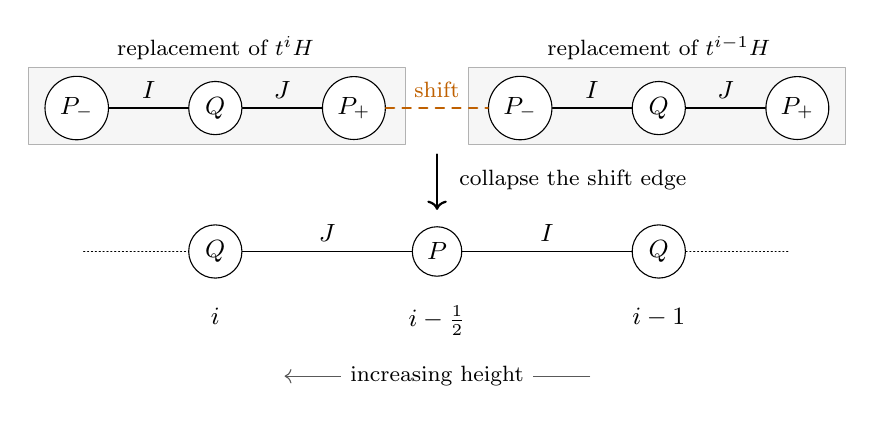
\begin{tikzpicture}[x=.88cm,y=.88cm,font=\small,
 every node/.style={align=center},line cap=round,line join=round,
 row/.style={draw,circle,fill=white,inner sep=3pt}]
 \filldraw[fill=gray!7,draw=gray!60] (.1,3.7) rectangle (5.55,4.8);
 \filldraw[fill=gray!7,draw=gray!60] (6.45,3.7) rectangle (11.9,4.8);
 \node[font=\footnotesize] at (2.8,5.08) {replacement of $t^iH$};
 \node[font=\footnotesize] at (9.2,5.08) {replacement of $t^{i-1}H$};
 \node[row] (pm) at (.8,4.22) {$P_-$};
 \node[row] (q) at (2.8,4.22) {$Q$};
 \node[row] (pp) at (4.8,4.22) {$P_+$};
 \node[row] (pms) at (7.2,4.22) {$P_-$};
 \node[row] (qs) at (9.2,4.22) {$Q$};
 \node[row] (pps) at (11.2,4.22) {$P_+$};
 \draw (pm)--node[above] {$I$} (q);
 \draw (q)--node[above] {$J$} (pp);
 \draw[thick,dashed,orange!75!black]
   (pp)--node[above,font=\footnotesize] {shift} (pms);
 \draw (pms)--node[above] {$I$} (qs);
 \draw (qs)--node[above] {$J$} (pps);
 \draw[->,thick] (6,3.55)--(6,2.75);
 \node[anchor=west,font=\footnotesize] at (6.18,3.18)
   {collapse the shift edge};
 \node[row] (aq) at (2.8,2.15) {$Q$};
 \node[row] (ap) at (6,2.15) {$P$};
 \node[row] (aqs) at (9.2,2.15) {$Q$};
 \draw[densely dotted] (.9,2.15)--(aq);
 \draw (aq)--node[above] {$J$} (ap);
 \draw (ap)--node[above] {$I$} (aqs);
 \draw[densely dotted] (aqs)--(11.1,2.15);
 \node[below=7pt] at (aq.south) {$i$};
 \node[below=7pt] at (ap.south) {$i-\tfrac12$};
 \node[below=7pt] at (aqs.south) {$i-1$};
 \draw[->,gray!70!black] (8.2,.35)--(3.8,.35);
 \node[font=\footnotesize,fill=white] at (6,.35) {increasing height};
\end{tikzpicture}
\caption{A local part of the actual row refinement. Each coarse row is
replaced by $P_-*_{I}Q*_{J}P_+$. The original shift edge has
isomorphisms at its two $P$-endpoints and can be collapsed; the $I$-
and $J$-edges remain. The heights shown below agree with $h(t)=1$.
Each displayed group is in the actual conjugate frame of its coarse
row. The picture shows a local path, not the whole Bass--Serre tree;
the quotient by $L$ is a line, while the actual tree can branch.}
\label{fig:row-refinement}
\end{figure}


\begin{lemma}[Row geometry and overlaps]\label{row:geometry}
All coarse and refined rows are hyperbolic, and their incident maps
are quasi-isometric embeddings. Refined rows are quasiconvex in their
containing coarse row \(H\). The coarse Magnus sides satisfy:
\begin{enumerate}[label=(\roman*)]
\item their ordinary intersection is \(F(B_0)\), or
\(F(B_0)*\langle w\rangle\) with \(w\) outside the common factor on
each side;
\item a conjugate intersection can be noncyclic only in the aligned
opposite-slot double coset; distinct same-slot cosets intersect at
most cyclically;
\item the overlap and its shifted copy have full-row-rank Fox matrices
in their free sides. They are strongly inert there: for every
finitely generated subgroup \(U\) of a free side \(P\), with overlap
\(O\le P\),
\[
 \sum_{UgO\in U\backslash P/O}
 \max\{\rk(U\cap gOg^{-1})-1,0\}
 \le \max\{\rk U-1,0\}.
\]
Proposition~\ref{row:path-inertia} proves the simultaneous
subgroup-homology injection behind this inequality from the stated
matrix property.
\end{enumerate}
In a nonfree root row \(Q\), \(z\) is not a proper power in the free
base. Distinct cyclic incidences at a free-base vertex of its root
splitting consequently have trivial intersection.
\end{lemma}

\begin{proof}
The one-relator group \(H\) embeds in \(G\) and contains no
Baumslag--Solitar subgroup, so it is hyperbolic by
\cite[Theorem~1.1]{OpenAIHyperbolicity}. Its Magnus sides are
quasiconvex \cite[Theorem~4.7]{LintonHyperbolic2026}.
Collins's ordinary-intersection theorem gives (i)
\cite[Theorem~2]{Collins2004}, and his conjugate-intersection theorem
gives (ii), including the case of equal Magnus subgroups
\cite[Theorem~2]{Collins2008}; see also
\cite[Section~8.3]{OpenAIHyperbolicity}.
The common alphabet is a connected Magnus subgraph.

For (iii), the Fox matrix keeps the identity columns for \(B_0\).
If \(w\) occurs, its derivative in the missing extreme letter is
nonzero: in a reduced word in a free group the relevant prefix
vertices are distinct, so those signed terms cannot cancel.
The matrix is triangular with a nonzero final pivot.
This supplies the matrix input for the induced-module restriction
argument below; the simultaneous rank bounds will follow from that
argument.

Each refined edge is finitely generated in a quasiconvex free
\(P\)-group, and hence is quasiconvex in \(H\). In a finite splitting
over ambient quasiconvex edge groups, the vertex groups are also
undistorted: replace successive excursions of a geodesic outside
a chosen vertex space by paths in the attaching edge cosets.
Ambient edge undistortion bounds their lengths linearly. This proves
quasiconvexity of the refined vertex groups in \(H\).

If \(|d|=1\), the root row is free. Otherwise, an equality \(z=v^m\)
with \(|m|>1\) would, by amalgam normal form, embed
\(\langle v,u\mid v^m=u^d\rangle\) into \(Q\).
Its central common power, together with a lift of an infinite-order
element of \(C_{|m|}*C_{|d|}\), generates \(\mathbb Z^2\).
This contradicts hyperbolicity. Thus \(\langle z\rangle\) is maximal
cyclic and malnormal in the free base.
\end{proof}

\subsection{Coefficients and level homology}

\begin{notation}\label{row:coefficients}
For \(U\leq G\), let \(D_U\) be the rational Linnell division field
inside the affiliated-operator algebra \(\mathcal U(U)\).
Local indicability and the strong Atiyah theorem give these compatible
Hughes-free fields
\cite{Brodskii1984,Howie1982,JaikinLopezAlvarez2020}.
We use natural subgroup embeddings, independence of distinct cosets
over subgroup fields, and rational skew-Laurent extension over the
kernel of a cyclic quotient
\cite[Section~2.3 and Proposition~2.2]{JaikinUniversality2021}.
Coset independence also holds for
affiliated coefficients: clear finitely many coefficients to bounded
subgroup operators and use their disjoint Fourier supports.

For \(V\leq U\), \(H_*(V;D_U)\) uses right group multiplication on
coefficients and left vector spaces; equivalently compute over
\(D_V\) and extend scalars. Put
\[
 \beta(V)=\dim_{D_V}H_1(V;D_V).
\]
This dimension is unchanged by overfield extension. For a nontrivial
free group of finite rank \(r\), it is \(r-1\); for an infinitely
generated free group it is infinite; for the trivial group it is zero.

Coefficients precede chain vectors and boundary matrices act on the
right. Write \(d(v)\) for the Fox one-chain of a word \(v\), so that
\[
 d(vw)=d(v)+v\,d(w),\qquad \partial d(v)=v-1,\qquad
 \Delta(v)=(v-1)^{-1}d(v)\quad(v\neq1).
\]
Thus \(\partial\Delta(v)=1\), and \(\Delta(v)-\Delta(w)\) is a cycle.
Intrinsic expressions are taken modulo two-boundaries.
A subgroup \emph{detects} a noncyclic subgroup in ambient homology
if some such difference from the latter subgroup has nonzero class.

Changing an orbit representative by \(s\) conjugates the group
symbols by \(s\) and right-multiplies their coefficients by \(s^{-1}\).
Conjugation of symbols and coefficients acts on ambient homology by
left multiplication by \(s\), so this convention preserves ambient
classes. Differentiating \(svs^{-1}\) gives the same verification:
connecting-path terms cancel for a cycle.
\end{notation}

Every noncyclic subgroup of a free group detects noncommensurable
elements. Indeed the support realization of
Section~\ref{sec:04-coefficients} places the normalized Fox chains
near their respective cyclic axes. Those axes have bounded overlap
when they are noncommensurable. Equality would give a finitely
supported chain with boundary the mass at the identity, contrary
to the zero total augmentation of a finite boundary.

The height-kernel presentation is
\begin{equation}\label{row:height-presentation}
 L=\langle a_i\ (i\in\mathbb Z)\mid R_i\ (i\in\mathbb Z)\rangle,
\end{equation}
where \(R_i\) is the shifted relator on \(a_i,\ldots,a_{i+k}\).
It comes from the infinite cyclic cover of the aspherical one-relator
complex \cite{Lyndon1950}, after collapsing its stable-letter tree.

\begin{lemma}[Level basis]\label{row:level-basis}
Over \(D_L\), the two-boundary in
\eqref{row:height-presentation} is injective. Every interval of \(k\)
consecutive \(a\)-columns is a basis of \(C_1/\im\partial_2\).
The corresponding quotient for any refined row, after extension to
\(D_L\), maps isomorphically to the global quotient. The incident
edge-to-row maps are isomorphisms on these quotients, and
\[
 \dim_{D_L}H_1(L;D_L)=k-1.
\]
\end{lemma}

\begin{proof}
Adjoin \(u_i\) at each index. In the first form replace \(R_i\) by
\(x_i=u_i^d,\ y_i=u_i^n\); in the second form use
\(u_i^d=z_i,\ x_iy_i=u_i^n\).
These are the elementary expansions and substitutions supplied by
the primitive change of basis. For \(m\neq0\), the \(u_i\)-derivative
of \(u_i^m\) is nonzero and hence is a unit over \(D_L\).
Eliminate the \(u_i\)-column. The resulting relation has nonzero
entries at both extreme \(a\)-columns, from the missing-letter
derivatives of \(x_i,y_i\) in their free sides.

In any finite dependence between shifted two-boundaries, an
outermost nonzero coefficient has an extreme entry which cannot
cancel. Hence the two-boundary is injective. Conversely either
extreme column can be eliminated using that shifted relation.
Repeated elimination moves any finite chain into a prescribed
\(k\)-letter interval. A dependence within that interval would trim
from both ends of a finite filling and force every relator coefficient
to vanish. This proves the basis assertion.

For \(P\)-rows this is the alphabet basis. The free tuples
\((B_0,x)\) and \((B_0,y)\) give triangular changes of basis with
nonzero extreme pivots. In a root row, first quotient by its root
relation using the unit \(u\)-entry, and then make this triangular
change. The first form uses the two power pivots instead. This proves
the other row assertions. Conjugate rows add connecting Fox paths,
whose coefficients cancel on cycles.

The boundary of the resulting \(k\)-dimensional quotient is onto
\(D_L\), because \(v-1\) is a unit for \(1\neq v\in L\).
Its kernel has dimension \(k-1\).
\end{proof}

\begin{proposition}[Restriction to row orbits]\label{row:restriction}
For \(U\leq L\) and an actual level \(\mathscr L\), inclusion and the
above coefficient transport give an injection
\begin{equation}\label{row:level-restriction}
 \bigoplus_{\xi\in U\backslash\mathscr L}
 H_1(U\cap X_\xi;D_U)\ \longrightarrow\ H_1(U;D_U).
\end{equation}
For \(U\) in a vertex row, the analogous sum over one incident slot
injects. The same assertions hold for coarse rows. The assertions
hold in the induced chain modules before passing to an overfield.
\end{proposition}

\begin{proof}
Use
\[
 E_U=D_U\otimes_{\mathbb QU}\mathbb QL,
\]
embedded in \(D_L\) by coset independence. Its restriction to a row,
the double-coset decomposition, and Shapiro's lemma give precisely
the summands of \eqref{row:level-restriction}
\cite{Brown1982,Serre1980}. Thus we must check that a row cycle
bounding over \(E_U\) already bounds in the row over the same module.
For a free row, this is the column-independence argument.

For a root row keep the added columns \(u_j\), so that no division
inside \(E_U\) is needed. A \(Q\)-chain at index \(i\), with free base
\((B_0,x)\), uses its common alphabet, the word \(x_i\), and \(u_i\),
but not the other extreme letter. Trim a finite filling from its
outermost index \(j\neq i\). There the relation \(x_jy_j=u_j^n\)
has a nonzero extreme-letter entry not otherwise used at that end.
Its coefficient is zero in \(D_L\), and therefore in \(E_U\).
The \(u_j\)-column next kills the coefficient of \(u_j^d=z_j\).
Repeat from both ends. At the remaining index \(i\), the unused
extreme letter kills the \(x_iy_i=u_i^n\) coefficient. What remains
is exactly the row's root relation, with its original coefficient
in \(E_U\). Substitution for \(x_i\) is injective by its nonzero
missing-letter entry. Hence it is already a row filling.
The first form and the coarse \(H\)-row use the same paired-column
or extreme-column trimming.

For a single slot replace \(L\) by the vertex group in this argument.
At a free vertex the attaching free tuple has full Fox rank; at a
root vertex the root column gives the extra pivot. The overfield is
used only to infer that a coefficient multiplying a nonzero entry
vanishes, never to divide within \(E_U\). This also proves the
assertion about induced modules.
\end{proof}

\begin{proposition}[Path inertia]\label{row:path-inertia}
In \(T\) and \(T_0\), every path with noncyclic pointwise stabilizer
is monotone. For each fixed monotone shape in a fixed absolute level
range, the first homologies of
its stabilizers, indexed modulo \(L\), inject jointly into
\(H_1(L;D_L)\). A path containing an edge has finitely generated free
stabilizer, and a fixed finite shape has finitely many \(G\)-orbits
with nontrivial stabilizer, or finitely many \(L\)-orbits when its
absolute level range is fixed. In particular
\begin{equation}\label{row:rank-budget}
 \sum_{\gamma\bmod L}\max\{\rk\Stab(\gamma)-1,0\}\leq k-1.
\end{equation}
The same joint-injection statement holds for continuations of any
fixed additional shape inside any subgroup \(U\) of a current path
stabilizer, with the intersection summands indexed by \(U\)-orbits.
It holds after restriction of the actual induced matrices and
double-coset decompositions, not just as a numerical inequality.
\end{proposition}

\begin{proof}
Apply the slot rule with \(U\) an incident edge group. The identity
edge orbit already accounts for all of \(H_1(U;D_U)\).
Every different same-slot intersection has zero first field
homology, so, being free, is trivial or cyclic. A reversal of a
reduced path passes through two such edges. This proves monotonicity
in \(T\). The coarse argument is the same, or follows from the
equal-Magnus-subgroup intersection theorem. Inserting collapsed shift
edges at successive \(P\)-passages takes a long monotone refined
path to a long monotone coarse path.

Begin at a free side and extend a monotone path one step in either
direction. Only the aligned opposite-slot double coset can have a
noncyclic intersection, by Lemma~\ref{row:geometry}(ii).
Its overlap \(O\leq P\) has a full-row-rank Fox matrix.
For arbitrary \(U\leq P\), perform this calculation over
\(D_U\otimes_{\mathbb QU}\mathbb QP\).
Injectivity on cycles, followed by its double-coset decomposition,
gives the simultaneous injection for all
\(U\cap sOs^{-1}\). Other continuation double cosets are cyclic and
have zero first homology. Repeat for each current stabilizer at
the next step. This proves both the global injection and the
asserted arbitrary-subgroup version. The intervening refined steps
use Proposition~\ref{row:restriction}.

This keeps the subgroup matrices throughout: restriction to a
smaller subgroup merely decomposes the same induced modules again.
If an independent finite family of the resulting cycles acquired
an ambient relation, the trimming proof of
Proposition~\ref{row:restriction} would reduce it to a relation at
the preceding step. This supplies the restriction property used
later for different double-coset orbit summands.

At each step, intersect quasiconvex subgroups in a hyperbolic row.
Their intersections are finitely generated and quasiconvex, and
only finitely many double cosets have nontrivial intersection.
Iterating over a fixed shape gives the claimed finite lists.
Each path group lies in a free edge group and is free.
The joint injection and Lemma~\ref{row:level-basis} prove the budget.
\end{proof}

We will use more than the numerical budget. Inside a later path group,
a predecessor already contributing its full first homology excludes
a second noncyclic predecessor orbit. The induced-module statement
also retains the distinction between different double cosets after
restriction to a subgroup. These are the two forms of path inertia
used in the trajectory construction of Section~\ref{gate:trajectory-clusters}.
If \(k=1\), the budget is zero and no path containing an edge has a
noncyclic stabilizer; the next lemma then gives the acylindrical case.

\begin{lemma}[Cyclic-path dictionary]\label{row:cyclic-dictionary}
Fix a finite edge-containing path shape. In a reduced tree path
fixed pointwise by a nontrivial element, the number of pairwise
disjoint subsegments of that shape having cyclic stabilizer is
bounded. Monotonicity is not required.
\end{lemma}

\begin{proof}
The fixed shape has finitely many nontrivial stabilizer \(G\)-orbits;
record traversal directions as well. Too many such subsegments
give an element \(s\) taking an earlier one to a later one with
direction preserved. Both cyclic stabilizers contain the common
nontrivial element \(c\). Thus \(s\) commensurates \(\langle c\rangle\).
The commensurator is cyclic in a torsion-free hyperbolic group.
It is elliptic in this tree, since it contains a nonzero power
fixing the first segment. But taking an oriented edge forward to
one pointing the same way on a geodesic is tree-hyperbolic: the
intervening segment and its successive translates concatenate
without backtracking into an axis. This contradiction gives the bound.
\end{proof}

\subsection{Subtree gates and finite homology in a row}

The path-homology estimate is now available. We turn to the second
output of this section: recognizing when a periodic subgroup is
quasiconvex in \(G\). First we give a geometric criterion for a
subgroup carried by a finite-quotient subtree. Finite row homology
will then supply its local hypotheses, and the period rule will
supply the subtree.

\begin{lemma}[Subtree gate criterion]\label{row:boundary-gates}
Let a torsion-free hyperbolic group \(J\) act cocompactly on a tree
of hyperbolic Cayley spaces with uniformly quasi-isometrically
embedded edge maps and hyperbolic total space. We use the standard
Cayley realization with uniformly proper vertex inclusions and
isometric product strips over open edges. For the finite splittings
here, properness is uniform: normalize a vertex to the identity and
take the maximum intrinsic length of the finitely many elements in
each ambient word ball, over the finitely many vertex types.
Let \(A\leq J\) preserve a connected subtree \(Y\), with
\(A\backslash Y\) finite. Suppose its vertex and edge stabilizers
are finitely generated and quasiconvex in the respective rows.
Either of the following suffices for \(A\) to be quasiconvex in \(J\):
\begin{enumerate}[label=(\roman*)]
\item ambient vertex rows are quasiconvex in \(J\);
\item every edge leaving \(Y\) intersects \(A\) trivially or cyclically.
\end{enumerate}
This applies in particular to \(G\) acting on \(T\) or \(T_0\).
\end{lemma}

\begin{proof}
At every included vertex \(v\), take a connected quasiconvex
neighborhood of an orbit of \(A_v=A\cap J_v\). Connect these
neighborhoods across included edges by strips over edge-intersection
orbits. The attachment offsets have finitely many types modulo \(A\).
The resulting connected path space \(W\) is proper and \(A\)-cobounded,
and is quasi-isometric to \(A\). We construct a coarse Lipschitz
retraction from the total space to \(W\).
Here an intersection orbit means the orbit of the intersection of
the two stabilizers through a chosen attachment point. The literal
cosets need not meet: fixed bounded connecting paths are included
in the attachment data. All statements about gates and intersections
below allow these bounded offsets.

Inside an included vertex take coarse nearest-point projection to
its orbit neighborhood. These projections agree across an included
edge through their gates to its exact intersection subgroup.
Indeed a geodesic in the attaching hull to a point of the intersection
passes close to the vertex gate. It stays near the attaching hull,
placing that gate in a bounded-neighborhood overlap.
For two fixed subgroup cosets such an overlap is within bounded
distance of their intersection orbit: properness leaves finitely many
possible discrepancies of a close pair, and pairs with one fixed
discrepancy form an orbit of the intersection subgroup.
First-entry gates in the edge thus coarsely agree with both vertex
gates. Quasi-isometric edge maps preserve this description by
quasigeodesic stability. There are finitely many included attachment
types, so the bounds are uniform and are measured in the intrinsic
path metric of \(W\).

Each omitted tree component attaches across one edge. In case (i)
the vertex subgroup at that edge is quasiconvex in \(J\).
Ambient projection to its orbit extends the gate throughout the
omitted component, agreeing at the boundary up to bounded error.
Its target metric is also intrinsic to the subgroup orbit. This
proves case (i).

For case (ii), consider an omitted attaching hull in the included
boundary row. Its projection to the vertex-subgroup neighborhood
has bounded diameter, or is within bounded distance of an orbit of
their cyclic intersection. The alternatives are uniform. To see
this, write the vertex subgroup as \(M\) and an attaching coset as
\(gE\), where \(E\) belongs to the finite list of incident edge
types. A projection of sufficiently large diameter forces a close
pair \(p\in M\), \(q\in gE\), by thin quadrilaterals. Translate by
\(p^{-1}\in M\). The pair becomes \((1,s)\), with \(s\) in a fixed
finite intrinsic word ball, and the attaching coset becomes \(sE\).
There are therefore only finitely many such configurations modulo
\(M\). In each one, pairs at a fixed bounded discrepancy form an
orbit of \(M\cap sEs^{-1}\); the finitely many discrepancies give
the bounded connecting offsets described above. Hence the projection
lies uniformly near the intersection orbit. Trivial intersections
give bounded projections, and the unbounded cases have finitely
many cyclic types.

A bounded projection extends by a constant. In an unbounded case
choose a generator \(c\) of the cyclic intersection and its periodic
axis coordinate. Let \(f\) be the gate coordinate on the attaching
hull. Projection first to the quasiconvex \(M\)-orbit and then to
this axis agrees, up to a uniform error, with direct intrinsic
projection to the axis: the first projection lies near the cyclic
intersection orbit, and thin triangles compare the two gates.
The boundary row itself may be distorted in \(J\), so its intrinsic
Lipschitz estimate does not suffice. We claim in the ambient metric that
\begin{equation}\label{row:ambient-line-bound}
 |f(x)-f(y)|\leq C\,d_J(x,y)+C.
\end{equation}
The inclusion of the boundary vertex row has a Cannon--Thurston
extension \cite[Corollary~3.11]{Mitra1998}, since the splitting has
finite quotient, hyperbolic vertex and edge groups, and
quasi-isometrically embedded edge maps. Its periodic-axis endpoints map to the
two distinct endpoints of \(c\) in \(\partial J\).
For each normalized cyclic configuration there exist \(M_0,R_0\)
such that, whenever the intrinsic gate coordinates of \(x,y\) lie
on opposite sides of the origin with margins at least \(M_0\), an
ambient geodesic between them meets \(B_J(1,R_0)\). Otherwise choose
pairs with both margins at least \(n\) and ambient geodesics missing
\(B_J(1,n)\). Thin triangles make the two sequences converge to the
opposite intrinsic axis endpoints: their Gromov products with those
endpoints tend to infinity even when their off-axis legs do also.
Cannon--Thurston continuity gives the two distinct ambient endpoints
of \(c\) as their limits. But avoidance of \(B_J(1,n)\) makes their
mutual ambient Gromov products tend to infinity, forcing the same
limit, a contradiction. Taking maxima over the finite list makes
\(M_0,R_0\) uniform.

Consequently an ambient geodesic from \(x\) to \(y\) passes uniformly
near every intervening \(c^j\), outside fixed endpoint margins.
Indeed recenter by \(c^{-j}\) and apply the preceding assertion.
The constants are independent of \(j\) by cyclic translation. The cyclic orbit
is undistorted in \(J\). Choose a uniformly spaced subcollection of
those translates with disjoint, positively separated fixed-radius
balls. A geodesic meeting all those balls has length at least a
constant times their number. This proves
\eqref{row:ambient-line-bound}.

On the discrete attaching hull enlarge the constant so that \(f\)
is Lipschitz (or replace it within bounded distance by a Lipschitz
function). Extend it over the outside component by the metric
inf-envelope
\[
 \widetilde f(z)=\inf_x\{f(x)+C\,d_J(x,z)\}.
\]
Round its values to integers and send them to the same periodic
orbit. This gives a coarse Lipschitz extension in the intrinsic
target metric, agreeing with the attaching gate up to bounded
error. Only the cyclic coordinate has been estimated in the
ambient metric; undistortion of the boundary row was not assumed.

Combine these extensions with the compatible included-vertex
gates. Across every ordinary or strip edge the image distance
in \(W\) is uniformly bounded, giving a global coarse Lipschitz
retraction. Since \(W\) is quasi-isometric to \(A\), the retraction
proves ambient undistortion, and hence quasiconvexity in \(J\).
\end{proof}

\begin{lemma}[Finite homology in a refined row]\label{row:row-finiteness}
Every subgroup \(M\) of a refined row with \(\beta(M)<\infty\) is
finitely generated and quasiconvex in that row. If \(\beta(M)=0\),
then \(M\) is trivial or cyclic.
\end{lemma}

\begin{proof}
For a free row this follows from the free-group rank formula.
Consider a nonfree root row
\[
 Q=F(B_0,x)*_{\langle z\rangle=\langle u^d\rangle}\langle u\rangle
\]
and restrict its cyclic splitting to \(M\).
All edge first homologies vanish. The tree Mayer--Vietoris sequence
injects the sum of vertex first homologies into \(H_1(M;D_M)\).
Thus all free-base vertex stabilizers are finitely generated, and
only finitely many orbits of them are noncyclic.

At a cyclic free-base stabilizer, at most one incident edge has
nontrivial intersection, and its maximal-cyclic property implies
that this whole vertex stabilizer fixes that edge. At a noncyclic
free-base stabilizer, quasiconvexity in the free base gives finitely
many orbits of nontrivial edge intersections. Root-side vertices
have valence \(|d|\).
Hence each component of nontrivially stabilized edges has finite
quotient and finitely generated stabilizer: a path between root-side
vertices must pass through a noncyclic free-base vertex, while
cyclic free-base vertices are leaves. There are only finitely many
noncyclic vertex orbits and finitely many relevant incidences at each.

Collapse these components and split over the remaining trivial
edges. Bass--Serre normal form expresses \(M\) as a free product of
their nontrivial stabilizers, remaining nontrivial vertex stabilizers,
and a free group. The case \(M=1\) is immediate. For \(M\neq1\),
with \(s\) nontrivial factors and free rank \(r\), the field homology
dimension is
\[
 \sum_{j=1}^{s}\beta(M_j)+s+r-1.
\]
Infinitely many factors or free generators give infinite dimension,
as follows either by finite subproducts or the degree-zero part of
the tree sequence. Finite \(\beta(M)\) therefore gives a finite
graph-of-groups core and finite generation.

If \(\beta(M)=0\), no free-base stabilizer is noncyclic.
Each nontrivial-edge component is then a finite star whose cyclic
leaves collapse into its root-side cyclic group.
The free-product formula leaves only the trivial or cyclic case.

The free-base and cyclic vertices of the root splitting are
quasiconvex in \(Q\): the cyclic edge is ambient quasiconvex, and
the excursion argument of Lemma~\ref{row:geometry} applies.
The vertex groups of the finite \(M\)-core are quasiconvex there,
as are the edge groups. Lemma~\ref{row:boundary-gates}(i) proves
quasiconvexity of \(M\) in \(Q\).
\end{proof}

\subsection{Periodicity and the homology budget}

\begin{proposition}[Period rule]\label{row:period-rule}
Suppose \(A\leq G\), \(h(A)\neq0\), and
\[
 S=A\cap L,\qquad 0<\beta(S)<\infty.
\]
At every actual level \(\mathscr L\), inclusion induces an isomorphism
\[
 \bigoplus_{\xi\in S\backslash\mathscr L}
 H_1(S\cap X_\xi;D_S)\ \longrightarrow\ H_1(S;D_S).
\]
Both incident edge-level maps to a vertex level are isomorphisms.
Every level sum therefore has dimension \(q_X=\beta(S)\).
The convex hull \(Y\) of the rows with noncyclic \(S\cap X_\xi\)
contains no edge with trivial \(S\)-stabilizer.
If \(A\) is also finitely generated, then \(A\backslash Y\) is finite
and \(A\) is quasiconvex in \(G\).
\end{proposition}

\begin{proof}
Use \(D_S\)-coefficients. Let \(V_j\) be the summed vertex homology
at the \(j\)-th vertex level and \(E_j\) the sum at the intervening
edge level. Proposition~\ref{row:restriction} makes these finite
dimensional and both maps \(E_j\to V_j,V_{j+1}\) injective.
The cokernel \(C\) of the edge-to-vertex first-homology map in
the tree sequence injects into \(H_1(S;D_S)\).

For an interval \([a,b]\) set
\[
 C[a,b]=\left(\bigoplus_{j=a}^{b}V_j\right)/
             \im\left(\bigoplus_{j=a}^{b-1}E_j\right).
\]
It injects into \(C\). Indeed any exterior finite-support relation
trims at its outermost edge, since the map to that outer vertex
is injective, leaving only the relations already imposed.
The same trimming makes the internal edge map injective. Thus
\[
 \dim C[a,b]=\dim V_a+
       \sum_{j=a}^{b-1}\bigl(\dim V_{j+1}-\dim E_j\bigr).
\]
Each summand is nonnegative. A positive-height element of \(A\)
periodically identifies these data, semilinearly over \(D_S\).
A positive summand would recur indefinitely and contradict
\(\dim C\leq\beta(S)<\infty\).
Expanding intervals in the other direction proves surjectivity
onto \(V_j\) as well. All adjacent maps are isomorphisms and each
level maps isomorphically to \(C\).

The remaining part of the tree sequence is
\[
 K_0=\ker\left(
 \bigoplus_{\text{edge orbits}}H_0(S_e;D_S)
 \longrightarrow
 \bigoplus_{\text{vertex orbits}}H_0(S_v;D_S)\right).
\]
It is a quotient of \(H_1(S;D_S)\) and hence finite dimensional.
A nonzero vector in \(K_0\) has finite level support. Sufficiently
spaced height translates would give linearly independent vectors
with disjoint supports. Thus \(K_0=0\), and \(H_1(S;D_S)=C\).

Take the actual path between rows with noncyclic stabilizer.
Its edge chain with coefficient \(1\) has boundary supported at
those endpoints, whose \(H_0\)'s vanish. If the path contained
a trivially stabilized edge, its orbit coefficient would be a
nonzero signed sum of distinct group monomials: distinct actual
edges with trivial stabilizer have distinct transporters, and a
tree path repeats no edge. It would therefore yield a nonzero
vector in \(K_0\), a contradiction. This proves the hull assertion.

By Lemma~\ref{row:row-finiteness}, all row intersections are finitely
generated and quasiconvex; every noncyclic one contributes at least
one dimension. The level bound and height periodicity give finitely
many \(A\)-orbits of such rows. When \(A\) is finitely generated,
join a base vertex to its translates under a finite generating set
and to representatives of these finitely many row orbits.
All \(A\)-translates of these paths form an invariant tree of finite
quotient containing \(Y\). Hence \(A\backslash Y\) is finite.

At a boundary edge, the \(A\)-stabilizer equals the \(S\)-stabilizer,
since row groups have height zero. A noncyclic edge intersection
would put both endpoints in \(Y\), so every leaving intersection
is at most cyclic. Apply Lemma~\ref{row:boundary-gates}(ii).
The finite-generation assumption has been used only for this last
cocompactness and quasiconvexity conclusion, not for the preceding
homology or nontrivial-edge assertions.
\end{proof}

\section{Support and descent for division-ring coefficients}
\label{sec:04-coefficients}

The closure construction requires two forms of algebraic coefficient
control. Disjoint subgroup support patterns must give independent
expressions. We also need descent from intersecting subgroup-field
spans when the subgroup intersection is separable in both groups.
Theorem~\ref{coeff:support} supplies these assertions.
Section~\ref{sec:analytic-localization} supplies the
separate localization argument for coefficients subject to height
translation.

Throughout this section, \(J\) is a locally indicable group and \(D_J\)
is its Hughes-free division ring over \(\Q\). For \(A\le J\), write
\(D_A\) for the division subring generated by \(\Q A\). We use the
subgroup inheritance and crossed-product properties of these fields:
if \(H\le J\) is finitely generated and
\(\chi\colon H\twoheadrightarrow\Z\) has kernel \(K\), then, choosing
\(t\in H\) with \(\chi(t)=1\),
\begin{equation}\label{coeff:cyclic-field}
 D_H=D_K(t;\operatorname{Ad}t)
 \ \hookrightarrow\ 
 D_K((t;\operatorname{Ad}t)).
\end{equation}
The left side is the Ore division ring of skew Laurent polynomials,
and the right side consists of series bounded below in degree. Distinct
subgroup cosets are independent over the corresponding subgroup field.
The normal-subgroup crossed-product assertion is
\cite[Section~2.3 and Proposition~2.2]{JaikinUniversality2021}; the
compatible rational affiliated realization is
\cite[Corollaries~6.2--6.3]{JaikinLopezAlvarez2020}, extending the
Hughes-free framework of \cite{Hughes1970}.

For arbitrary, possibly nonnormal $A$, coset independence follows
directly in that realization. If $\sum_i d_i g_i=0$ with
$d_i\in\mathcal U(A)$ and distinct right cosets $Ag_i$, put
$b=(1+\sum_i d_i d_i^*)^{-1/2}$. This is injective and all $bd_i$
are bounded. The bounded terms $bd_i g_i$ have disjoint Fourier
supports, so each is zero and hence each $d_i=0$. Left cosets use
a common right regularizer. This argument does not attribute
nonnormal coset independence to the normal-subgroup proposition.

Our arguments concern algebraic rational expressions and do not assign
Fourier coefficients to an arbitrary affiliated operator.

\subsection{Permitted support patterns}

A \emph{support pattern} is a subset of \(J\) of the form
\[
 \mathcal P=A_1g_1A_2g_2\cdots A_mg_m,
 \qquad A_i\le J,\quad g_i\in J.
\]
A product \(d_1g_1\cdots d_mg_m\), where \(d_i\in D_{A_i}\), is
\emph{permitted on} \(\mathcal P\). For \(S\subseteq J\), let
\(\mathcal V(S)\) be the \(\Q\)-span of all such products whose
support pattern is contained in \(S\). These are permitted algebraic
supports; no choice of a scalar-function realization is involved in the
definition. In particular,
\(\mathcal V(S)g=\mathcal V(Sg)\).

\begin{theorem}[Support and coset descent]\label{coeff:support}
The following assertions hold.
\begin{enumerate}[label=\textup{(\roman*)}]
\item If \(S\cap T=\varnothing\), then
\(\mathcal V(S)\cap\mathcal V(T)=0\).
\item There is a \(\Q\)-linear map
\[
 \mathcal F\colon D_J\longrightarrow\Q^J
\]
with \(\mathcal F(1)=\delta_1\), commuting with every right group
translation, such that
\(v\in\mathcal V(S)\) implies
\(\supp\mathcal F(v)\subseteq S\).
\item Let \(A,B\le J\) and \(C=A\cap B\). If \(At\cap Bs\) is empty,
then \(D_A t\cap D_B s=0\). Otherwise, for any \(x\in At\cap Bs\),
\begin{equation}\label{coeff:single-coset}
 D_A t\cap D_B s=D_Cx.
\end{equation}
If, in addition, \(C\) is separable in both \(A\) and \(B\), then
\begin{equation}\label{coeff:finite-span}
 \left(\sum_{g\in J}D_Ag\right)
 \cap
 \left(\sum_{g\in J}D_Bg\right)
 =\sum_{g\in J}D_Cg,
\end{equation}
where each sum denotes its algebraic, finite-support span.
\end{enumerate}
\end{theorem}

Applied entrywise to a finite row \(v\), the map in (ii) satisfies
\[
 \mathcal F(vR)=\mathcal F(v)R
 \qquad\text{for every compatible finite matrix }R\text{ over }\Q J.
\]
Indeed each matrix entry acts by a finite sum of right group
translations. Thus the same scalar-function map preserves the Fox
boundary and divergence equations used in the closure construction.
This consequence uses linearity and right equivariance; it requires
no multiplicativity for division-ring coefficients.

We first make the complexity argument precise. The two descent
arguments will use the same coefficient extraction, but have different
conclusions: disjoint supports give vanishing, while intersecting
single cosets give a smaller field.

\subsection{A hereditary complexity and coefficient extraction}

For predecessors of coefficient descent by rational-expression complexity,
see Dicks--Herbera--S\'anchez
\cite[Sections~3--6, especially Theorem~6.3]{DicksHerberaSanchez2004}
and Jaikin-Zapirain--L\'opez-\'Alvarez
\cite[Proposition~5.1]{JaikinLopezAlvarez2020}.
Here we combine an explicit ordinal complexity with bookkeeping for the
prescribed subgroup support patterns.

The difficulty in an induction is inversion. A coefficient of an
inverse series is a finite sum of products, but neither the lengths
of those products nor the number of their displayed terms has a
uniform bound. We therefore use two ordinal layers: the first makes
simplifying an inverse operand outweigh any finite increase in
product length, and the second makes simplifying a term outweigh
any finite increase in the number of terms. We define them on the
displayed expressions, retaining terms even when their values cancel.

A displayed rational expression can be normalized recursively as a
finite sum of terms
\begin{equation}\label{coeff:normal-term}
 q P_1^{-1}\cdots P_s^{-1}g,
 \qquad q\in\Q\setminus\{0\},\quad g\in J.
\end{equation}
Each \(P_i\) is a displayed sum in the same form, has nonzero value,
and has at least one top term with final offset \(1\). To obtain this
normalization before taking an inverse, choose a displayed top offset
\(g\), factor it to the right, and move the resulting monomial through
other inverse factors by conjugation. For example,
\(gP^{-1}=(gPg^{-1})^{-1}g\). These operations preserve the number and
nesting of inverse occurrences. They do not identify equal displayed
terms or cancel terms against one another.

The \emph{hereditary offsets} of an expression are all final group
elements appearing at any depth of its displayed expression tree.
For an inverse occurrence \(P^{-1}\), let \(H(P)\) be the subgroup
generated by the hereditary offsets of \(P\). Assign the term
\eqref{coeff:normal-term} the pattern
\begin{equation}\label{coeff:displayed-pattern}
 H(P_1)\cdots H(P_s)g.
\end{equation}
When the original factors have prescribed subgroup-field patterns,
normalize them separately before multiplying. Every resulting term
pattern is then contained in its original prescribed pattern.
Indeed all offsets used to represent an element of \(D_A\) can be
chosen in \(A\); moving a monomial through a later factor conjugates
that factor's subgroup and moves the same monomial to the right.

Write \(\oplus\) for natural, or Hessenberg, addition of ordinals:
add the coefficients of equal powers in Cantor normal form. Define the
\emph{path weight} and \emph{complexity} recursively by
\begin{align}
 w(qP_1^{-1}\cdots P_s^{-1}g)
   &=\bigoplus_{i=1}^s\omega^{c(P_i)},\label{coeff:path-weight}\\
 c(E)&=\bigoplus_{T\text{ a displayed term of }E}\omega^{w(T)}.
 \label{coeff:complexity}
\end{align}
An empty sum has complexity zero. Every complexity here is a finite
hereditary ordinal below \(\varepsilon_0\). A monomial has weight zero;
a displayed sum of \(r\) monomials has complexity \(r\). Conjugating an
expression, changing a final monomial offset, or performing the preceding
normalization preserves these complexities. When an equality is under
consideration, its joint complexity counts all displayed terms on both
sides, including terms that cancel upon evaluation.

We shall use two elementary properties of this measure. Replacing an
occurrence of \(\omega^\alpha\) in a path weight by finitely many
\(\omega^{\beta_i}\), with every \(\beta_i<\alpha\), strictly decreases
that path weight. Replacing a displayed term of weight \(\eta\) by
finitely many terms of weights less than \(\eta\) strictly decreases
the outer complexity. Both statements follow directly from Cantor
normal form; unaffected summands may be retained by strict monotonicity
of natural addition. There is no bound on the finite number of replacement
terms. Also, the complexity of any inverse operand in a displayed
expression is strictly smaller than the complexity of the expression
containing it.

Relative to a character \(\chi\), call an inverse occurrence
\(P^{-1}\), or its normalized operand \(P\), \emph{nonhomogeneous}
when \(\chi\) is nonzero on some hereditary offset of \(P\),
equivalently on \(H(P)\). This refers to the displayed expression:
for example, \(1+t-t\) is nonhomogeneous when \(\chi(t)\ne0\),
although its value is constant. When all hereditary offsets are
killed by \(\chi\), the operand can instead be retained unchanged
in degree zero.

\begin{lemma}[Coefficient extraction invariant]\label{coeff:extraction}
Let finitely many normalized rational expressions have hereditary
offsets in a finitely generated subgroup \(H\), and let
\(\chi\colon H\twoheadrightarrow\Z\) be a character with kernel
\(K\). Expand in the positive skew Laurent field in
\eqref{coeff:cyclic-field}, writing powers of \(t\) on the right.
Every coefficient has a finite normalized rational expression in
\(D_K\), with the following properties.
\begin{enumerate}[label=\textup{(\alph*)}]
\item If a summand is permitted on \(S\), the expression for its
coefficient of degree \(n\) has term patterns contained in
\[
 (S\cap\chi^{-1}(n))t^{-n}.
\]
Here \(S\) can be replaced by its intersection with \(H\).
\item Coefficient extraction does not increase the complexity of an
arbitrary top expression. If an inverse occurrence is nonhomogeneous,
the decrease is strict. In particular, for a normalized operand \(P\)
whose hereditary offsets are not all killed by \(\chi\), every
coefficient expression has complexity strictly less than \(c(P)\).
\item For a collection of top expressions, assume at least one
represented top offset equals \(1\) and that \(\chi\) is nonzero on
the subgroup generated by all their hereditary offsets. The joint
complexity of the coefficient expressions at each degree is strictly
smaller than the original joint complexity.
\item If the input is represented in one field coset \(D_Aa\), with
all inverse operands internal to \(A\), a nonzero coefficient of
degree \(n\) is represented in one coset of \(D_{A\cap K}\). Its
permitted group coset is
\((Aa\cap\chi^{-1}(n))t^{-n}\), and its inverse operands remain
internal to \(A\cap K\).
\end{enumerate}
\end{lemma}

\begin{proof}
We construct the coefficients by induction on the expression trees.
An inverse operand whose hereditary offsets are all killed by
\(\chi\) is retained unchanged in degree zero. For any other inverse
operand \(P\), first use a transporter inside \(H(P)\): if
\(\chi(H(P))=d\Z\), choose \(a\in H(P)\) with \(\chi(a)=d>0\).
The cyclic-field property for this subgroup gives the expansion of
\(P\) in powers of \(a\). Its leading nonzero coefficient is itself
a rational expression. Factoring this coefficient and the leading
power gives the inverse expansion by the geometric series
\((1+R)^{-1}=\sum_{j\ge0}(-R)^j\), where \(R\) has positive
valuation. A fixed coefficient of that expansion is a finite sum of
finite products of coefficients of \(P\) and inverses of its leading
coefficient, with the conjugations imposed by the skew multiplication.
All series in this construction are bounded below, so coefficient
multiplication and inverse expansion involve only finitely many terms
in each fixed degree.

For completeness, the complexity comparison can be proved at the same
time by structural induction. A normalized nonhomogeneous operand
\(P\) has a top offset \(1\). If one of its inverse occurrences is
nonhomogeneous, the induction hypothesis decreases the complexities of
that occurrence's operand coefficients. If all its inverse occurrences
are homogeneous, every term contributes to just one degree, and the
nonzero character distinguishes at least two top offsets. Thus every
degree omits at least one term. These are the two cases proving that
every coefficient of \(P\) has complexity less than \(c(P)\).
Consequently, in expanding \(P^{-1}\), the inverse of its leading
coefficient has operand complexity less than \(c(P)\). Every inverse
operand appearing in one of the other coefficients also has complexity
less than \(c(P)\). Any coefficient term of \(P^{-1}\) therefore has
path weight less than \(\omega^{c(P)}\). This replaces the original
inverse's entire path contribution by finitely many lower contributions.
The two natural-sum comparisons above prove strict decrease even after
arbitrary finite multiplication and distribution of the coefficient
expressions. They also justify the nonhomogeneous-inverse case used
in the preceding structural induction.

This proves (b). For (c), retain the tags recording each original term.
If some inverse occurrence is nonhomogeneous, every resulting term
coming from that occurrence has smaller path weight, while unchanged
terms contribute at most once at any degree. If all inverse occurrences
are homogeneous, the top offset \(1\), together with nontriviality on
all hereditary offsets, forces another top degree. Every coefficient
then omits a top term. This proves (c), also for a joint collection
whose individual expressions need not have a top offset \(1\).

It remains to check that this construction respects the designated
supports rather than just the field identities. In the local expansion
at \(P^{-1}\), all transporters lie in \(H(P)\), and its coefficient
of height \(n\) is supported on the corresponding coset of
\(H(P)\cap K\). To compare with the global variable, write
\(a^m=k_m t^{dm}\), with \(k_m\in K\). A local coefficient then
acquires the final monomial offset \(k_m\). Moving powers of \(t\)
to the right in a product conjugates its subsequent kernel factors.
Multiplying the corresponding group elements shows that every resulting
term pattern is contained in the original product pattern's total-degree
slice, followed by \(t^{-n}\). The new offsets are monomials; their word
lengths play no role in \eqref{coeff:path-weight}--\eqref{coeff:complexity}.
Conjugations and final-offset changes preserve the measure. This proves
(a) and its compatibility with (b) and (c). For (d), all the local
transporters before the final offset lie in \(A\). When intermediate
global powers are moved to the right and the resulting monomials are
normalized, each conjugating prefix is consequently an element of
\(A\). It preserves \(A\cap K\), and the final offset lies in the
displayed single coset. This also follows by first expanding the whole
\(D_A\)-factor using an \(A\)-transporter and only then converting its
coefficients to the global variable.
\end{proof}

\subsection{Disjoint supports and the scalar-function map}

\begin{proof}[Proof of Theorem~\ref{coeff:support}(i)--(ii)]
Suppose \(v\in\mathcal V(S)\cap\mathcal V(T)\), with \(S\cap T\)
empty. Choose finite rational representations of its two values,
retaining the prescribed pattern for each top summand. We induct on
their joint complexity. Right-multiply the equality by the inverse of
one represented top offset. This translates both allowed sets and
preserves their disjointness and the joint complexity, while putting
one top offset at \(1\). Let \(H\) be the finitely generated subgroup
of all hereditary offsets in the shifted equality.

If \(H=1\), all nonzero displayed terms have pattern \(\{1\}\).
Disjointness forces one side to have no such term, and the equality
therefore has value zero. Otherwise local indicability gives an
epimorphism \(\chi\colon H\twoheadrightarrow\Z\). Apply
Lemma~\ref{coeff:extraction}. At each degree the two coefficient
expressions have strictly smaller joint complexity, and their allowed
supports are disjoint subsets of \(K\). The induction hypothesis
makes each side's coefficient zero. Injectivity of
\eqref{coeff:cyclic-field} makes both original values zero as well.
Well-foundedness of the ordinal measure completes the induction.

Set \(W=\mathcal V(J\setminus\{1\})\). Part (i) gives
\(W\cap\Q1=0\). Define a linear functional on \(W+\Q1\) by
\(\ell(w+q)=q\), and extend it to a \(\Q\)-linear functional on
\(D_J\). Put
\begin{equation}\label{coeff:scalar-map}
 \mathcal F(v)(g)=\ell(vg^{-1}).
\end{equation}
Then \(\mathcal F(1)=\delta_1\). If \(g\notin S\) and
\(v\in\mathcal V(S)\), then
\(vg^{-1}\in\mathcal V(Sg^{-1})\subseteq W\), so this coefficient
vanishes. Finally,
\[
 \mathcal F(vh)(g)=\ell(vhg^{-1})
   =\mathcal F(v)(gh^{-1}),
\]
which is precisely equivariance for right group multiplication.
This proves all support restrictions simultaneously. No multiplicativity
of \(\mathcal F\) is asserted or needed.
\end{proof}

\subsection{Rational descent from a smaller coefficient field}

We isolate the rational-series step, including its handedness.

\begin{lemma}[Rational descent]\label{coeff:rational-descent}
Let \(E\subseteq F\) be division rings and let conjugation by \(u\)
induce an automorphism of \(F\) preserving \(E\). If an element of
\(F(u)\) has a bounded-below Laurent expansion
\[
 S=\sum_n u^n f_n,\qquad f_n\in E,
\]
then \(S\in E(u)\).
\end{lemma}

\begin{proof}
Choose a nonzero right Laurent-polynomial denominator
\(P=\sum_{j\in I}u^jp_j\), with \(I\) finite and \(p_j\in F\),
such that \(SP\) is a Laurent polynomial. For all sufficiently large
\(n\), its coefficient of \(u^n\), with coefficients written on the
right, is zero:
\begin{equation}\label{coeff:recurrence}
 \sum_{j\in I}(u^{-j}f_{n-j}u^j)p_j=0.
\end{equation}
Every parenthesized coefficient belongs to \(E\). Choose a basis
\((b_\gamma)_\gamma\) of \(F\) as a \emph{left} vector space over
\(E\), and expand the finitely many coefficients as
\(p_j=\sum_\gamma e_{j\gamma}b_\gamma\). Only finitely many basis
vectors are used. Linear independence makes every coordinate tuple
\((e_{j\gamma})_{j\in I}\) satisfy all equations
\eqref{coeff:recurrence} simultaneously. Since \(P\ne0\), at least
one such tuple is nonzero. Fix it and put
\(P'=\sum_{j\in I}u^je_{j\gamma}\ne0\).

The product \(SP'\) has coefficients in \(E\), has a lower degree
bound, and vanishes in every sufficiently high degree. It is therefore
a Laurent polynomial over \(E\), and \(S=(SP')(P')^{-1}\in E(u)\).
There is no finite-subsystem argument here: one fixed coordinate tuple
satisfies the entire family of recurrence equations.
\end{proof}

\subsection{Intersections of field cosets}

\begin{proof}[Proof of Theorem~\ref{coeff:support}(iii), single cosets]
The empty-intersection assertion follows from part (i). Suppose
\(At\cap Bs=Cx\) and \(0\ne v\in D_At\cap D_Bs\). We induct on the
joint complexity of expressions for \(v\) in these two field cosets.
Choose all inverse operands on the first side inside \(A\), and all
those on the second inside \(B\). Right-shift by one represented top
offset as in the preceding proof, and let \(H\) be the subgroup
generated by the new hereditary offsets.

Intersect the two permitted cosets with \(H\). Each nonempty
intersection is a coset of \(A\cap H\), respectively \(B\cap H\).
All represented inverse operands remain internal to these subgroups:
their offsets lie in the original subgroup and, by definition, in
\(H\). Likewise, ratios of represented top offsets on a fixed side
lie in its intersected subgroup. Thus this restriction neither changes
the expression nor loses its single-coset form. The restricted cosets
have a common point by part (i), since their common field value is
nonzero. We may accordingly work entirely in \(H\), temporarily
reusing \(A,B,C\) for their intersections with \(H\).
If \(H=1\), the assertion is immediate.
Otherwise choose \(\chi\colon H\twoheadrightarrow\Z\), with kernel
\(K\).

For each degree \(n\), the two coefficient expressions lie in single
cosets of the fields of \(A\cap K\) and \(B\cap K\), allowing the
final offsets in \(K\) described in
Lemma~\ref{coeff:extraction}. Their joint complexity has strictly
decreased. The induction hypothesis therefore says that their common
value is zero if the two group cosets do not meet, and otherwise lies
in the field of \(A\cap B\cap K\) times a point of their
intersection. Returning to the original degree, the coefficient is
thus permitted precisely on the corresponding slice of the common
coset \(Cx\), with its subgroup-field coefficient in
\(D_{C\cap K}\).

Choose a common point \(x\) inside \(H\) and divide \(v\) by it on
the right. The resulting rational series has coefficients in the common
kernel field and group support restricted to \(C\). If
\(\chi(C)=0\), it has only degree zero and already belongs to
\(D_{C\cap K}=D_C\). If \(\chi(C)=d\Z\), with \(d>0\), choose
\(u\in C\) of height \(d\), and put
\(E=D_{C\cap K}\), \(F=D_K\). Then it has the form
\begin{equation}\label{coeff:common-series}
 vx^{-1}=\sum_m u^m f_m,\qquad f_m\in E,
\end{equation}
and conjugation by \(u\) preserves \(E\).

We must also check that \eqref{coeff:common-series} is rational over
\(F(u)\), not just over \(F(t)\). The subgroup
\(H_d=\chi^{-1}(d\Z)\) has index \(d\) in \(H\), and its field is
\(F(u)\). The finite crossed decomposition gives
\[
 D_H=\bigoplus_{r=0}^{d-1}D_{H_d}t^r.
\]
The Laurent series of the \(r\)-th summand uses only degrees congruent
to \(r\) modulo \(d\). Since \eqref{coeff:common-series} has only
zero-congruence degrees, injectivity of Laurent expansion makes all
other summands vanish. Hence \(vx^{-1}\in F(u)\).
Lemma~\ref{coeff:rational-descent} now gives
\(vx^{-1}\in E(u)=D_C\). This proves the required inclusion; the
reverse one follows from \(C\le A,B\). Undoing the initial common
right shift proves \eqref{coeff:single-coset} in the original frame.
If a restricted ambient subgroup was used, its common subgroup is
contained in the original \(C\), so this conclusion also gives the
original claim.
\end{proof}

\subsection{Finite spans and separability}

\begin{proof}[Proof of Theorem~\ref{coeff:support}(iii), finite spans]
One inclusion in \eqref{coeff:finite-span} is immediate. For the
other, write a common element as
\[
 v=\sum_{i=1}^{r}a_i t_i=\sum_{j=1}^{s}b_j s_j,
 \qquad a_i\in D_A,\quad b_j\in D_B.
\]
Merge repeated cosets on each side, so the original \(At_i\)'s are
pairwise disjoint, as are the \(Bs_j\)'s. Every nonempty overlap is
\(At_i\cap Bs_j=Cx_{ij}\).

For a fixed \(i\), two distinct overlaps \(Cx_{ij}\) and
\(Cx_{ik}\) have
\(x_{ij}x_{ik}^{-1}\in A\setminus C\). Separability supplies a
finite-index subgroup \(A_0\le A\) containing \(C\) and excluding
all these finitely many differences. Hence no right \(A_0\)-coset
inside \(At_i\) meets two distinct original \(B\)-cosets. To see
this independently of representatives, a common \(A_0\)-coset meeting
both overlaps would imply
\(c x_{ij}(c'x_{ik})^{-1}\in A_0\) for some \(c,c'\in C\), and
therefore \(x_{ij}x_{ik}^{-1}\in A_0\), a contradiction. Choose
\(B_0\le B\) symmetrically, of finite index and containing \(C\).

These two choices already give the simultaneous refinement required.
Since \(A_0\cap B=C\), the intersection of a refined \(A_0\)-coset
with its unique possible original \(B\)-coset is one \(C\)-coset.
As \(C\le B_0\), that entire intersection lies in just one refined
\(B_0\)-coset. The symmetric argument applies on the other side.
Thus the bipartite intersection graph of all refined cosets is a
matching, with possible isolated vertices. Also
\(A_0\cap B_0=C\).

We use the finite-index field decompositions
\[
 D_A=\bigoplus_{a\in A_0\backslash A}D_{A_0}a,
 \qquad
 D_B=\bigoplus_{b\in B_0\backslash B}D_{B_0}b.
\]
For clarity, these do not require the chosen subgroups to be normal.
One may first pass to a finite-index normal core: its finite crossed
span in the overfield is a finite-dimensional domain over its division
ring, hence a division ring, and so equals the larger subgroup field.
Grouping the resulting summands by the original subgroup cosets gives
the displayed formulas.

Refine the two expressions for \(v\) by these decompositions. Group
the terms of their difference according to the connected components
of the refined intersection graph. Distinct components have disjoint
unions of permitted supports. Part (i) therefore makes the value of
each component zero. Isolated terms vanish. Each remaining component
is a single pair, giving an equality between one \(D_{A_0}\)-coset
and one \(D_{B_0}\)-coset. By \eqref{coeff:single-coset}, their common
value belongs to \(D_Cx\) for a point of their group-coset overlap.
Adding the finitely many pairs proves \eqref{coeff:finite-span}.
\end{proof}

\section{Semilinear localization of affiliated coefficients}
\label{sec:analytic-localization}
\label{coeff:analytic}

Write \(\mathcal N(J)\) for the group von Neumann algebra of a discrete
group \(J\), with its canonical trace, and write \(\mathcal U(J)\) for
its algebra of affiliated operators.  The division fields used here are
embedded in these affiliated algebras. Our target is the following
localization statement for a finite semilinear coefficient system.

\begin{lemma}[Semilinear finite-dimensional support]
\label{coeff:analytic-support}
Let \(G\) be a torsion-free word-hyperbolic group, let
\(h:G\to\Z\) be a homomorphism, and put \(L=\ker h\).
Let \(D\le G\) be quasiconvex and put \(S=D\cap L\).
Choose \(g\in G\) and \(g_D\in D\) such that
\[
 h(g)=h(g_D)\ne0.
\]
Suppose that the division fields in use are embedded in the affiliated
group algebras, and that, for an integer \(r\ge1\), a row
\(\lambda\in D_L^{\,1\times r}\) satisfies
\begin{equation}\label{coeff:analytic-semilinear}
 g\lambda g_D^{-1}=\lambda B,\qquad
 B\in\operatorname{GL}_r(D_S).
\end{equation}
Then
\begin{equation}\label{coeff:analytic-support-conclusion}
 \lambda\in\sum_{xS\in\mathcal P}x\,\mathcal U(S)^{\,1\times r},
 \qquad
 \mathcal P=
 \{xS:\ x\in L,\ g^m\in xDx^{-1}
                    \text{ for some }m\in\Z\setminus\{0\}\}.
\end{equation}
The set \(\mathcal P\) is finite.  In fact, the same assertion holds
for any affiliated row \(\lambda\) and any affiliated invertible
matrix \(B\) satisfying \eqref{coeff:analytic-semilinear}.
\end{lemma}

Here is the normalization behind the proof. Put
\(\alpha=\operatorname{Ad}g_D\), and first consider the case in
which the map \(w\mapsto\lambda w\) on affiliated \(S\)-columns
has zero kernel. We seek a positive invertible affiliated matrix
\(P\) over \(S\) such that
\[
 P=B\alpha(P)B^*.
\]
Then
\[
 Z=\lambda P^{1/2},\qquad
 u=P^{-1/2}B\alpha(P)^{1/2}
\]
satisfy \(uu^*=u^*u=1\) and \(gZg_D^{-1}=Zu\).
Thus changing the positive form makes the coefficient transport
unitary. It follows that \(gZZ^*g^{-1}=ZZ^*\). Hyperbolicity and
the nonzero height of \(g\) will force this invariant affiliated
operator to be scalar, so every entry of \(Z\) is bounded.
These entries generate a closed right \(S\)-module in \(\ell^2(L)\)
of von Neumann dimension at most \(r\). Its invariance under height
translation excludes infinite
coset orbits from the support, and quasiconvexity of \(D\) leaves
only finitely many periodic cosets.

The invariant-form strategy parallels the bounded unitarization
argument of Sz.-Nagy and Dixmier
\cite[Section~5, Theorem~6]{Dixmier1950Means}.
The positive mean constructed below supplies \(P\). Its inputs
need not have a common operator-norm bound, so we average bounded
resolvent expressions and control the spectral tails of the inputs
and their inverses. When the column kernel is nonzero, the proof
first represents its complement by a projection over \(\mathcal N(S)\)
and carries out the same construction between the corresponding
corners.

The affiliated conclusion in \eqref{coeff:analytic-support-conclusion}
is sufficient for Proposition~\ref{close:join-injection}. There the
Bass--Serre homology injection is first established over a subgroup
division field. Extending scalars to its affiliated algebra preserves
that injection and its nonzero classes: choosing a vector-space
basis identifies the scalar extension with a direct sum of copies
of the nonzero affiliated algebra. Injectivity into ambient homology
still requires the separate comparison using actual row chains and
coset independence in that proposition.

\subsection{Measure estimates and a projection inequality}

Let \((\mathcal M,\tau)\) be a finite von Neumann algebra with a faithful
normal finite trace.  The trace need not have total mass one.  On matrices
we use the compatible \emph{unnormalized} traces
\[
 \tau_r((a_{ij}))=\sum_{j=1}^r\tau(a_{jj}).
\]
In particular, for a bounded rectangular matrix \(a\),
\(\tau_r(a^*a)=\tau_k(aa^*)\), with the appropriate source and target
matrix sizes.  Corners carry the restriction of these traces.  Products
and sums of affiliated operators mean their closed affiliated products
and sums.

A family \(\mathcal A\) of affiliated operators is \emph{tight} if
\[
 \lim_{K\longrightarrow\infty}
 \sup_{a\in\mathcal A}\tau\bigl(1_{(K,\infty)}(|a|)\bigr)=0.
\]
For rectangular operators the trace is taken in the source corner;
the nonzero spectral distributions of \(|a|\) and \(|a^*|\) agree
with the compatible traces.  We use convergence in measure: \(a_j\to0\)
if, for every \(\varepsilon,\eta>0\), eventually there is a projection
\(q\) with \(\tau(1-q)<\eta\) and \(\|a_jq\|<\varepsilon\).

\begin{lemma}[Measure calculus]\label{coeff:analytic-calculus}
The affiliated algebra of a finite von Neumann algebra is complete for
convergence in measure.  Products of tight families are tight.  If
\(a_j\to0\) in measure and \(b_j,c_j\) range over tight families, then
\(b_ja_jc_j\to0\) in measure.  These assertions also hold uniformly over
an additional index.

Positive square roots are continuous in measure on positive affiliated
operators, and inversion is continuous in measure on positive affiliated
units.  A uniformly norm-bounded family that tends to zero in measure
tends to zero in \(L^1(\tau)\); the same assertion holds uniformly.
\end{lemma}

\begin{proof}
The complete topological \(*\)-algebra assertion and the singular-number
estimates used below are the standard measurable-operator calculus;
see \cite[Sections~1.4--1.5, Lemma~2.5 and Lemma~3.1]{FackKosaki1986}.
For clarity, the estimates that provide all the uniformity we need are
\[
 \mu_{s+t}(ab)\le \mu_s(a)\mu_t(b),\qquad
 \mu_{s+t}(a+b)\le \mu_s(a)+\mu_t(b),
 \quad s,t>0,
\]
where
\[
 \mu_s(a)=
 \inf\{\|aq\|:\ q\text{ a projection},\ \tau(1-q)\le s\}.
\]
Their proofs cut the two operators to bounded parts and add the
trace codimensions; polar decomposition identifies the trace
codimensions of the source and range cuts.  Tightness says precisely
that \(\sup_{a\in\mathcal A}\mu_s(a)<\infty\) for every \(s>0\).
Convergence in measure says that \(\mu_s(a_j)\to0\) for every \(s>0\).
The two displayed estimates therefore prove the product and uniform
assertions.

We recall how to obtain the stated functional calculus without any
norm bounds on the original operators.  For positive \(a_j\to a\),
the resolvent identity and the product estimate give
\[
 (1+a_j)^{-1}-(1+a)^{-1}
 =(1+a_j)^{-1}(a-a_j)(1+a)^{-1}\longrightarrow0
\]
in measure.  On bounded self-adjoint contractions, polynomial
approximation gives continuity of continuous functional calculus in
measure.  Apply this to the positive contractions
\(q_j=(1+a_j)^{-1}\), with limit \(q=(1+a)^{-1}\).
Here is the endpoint control needed for unbounded scalar functions.
If \(q\) has no spectral atom at \(1\), then for every \(\eta>0\)
one can choose \(b<1\) with \(\mu_{\eta/2}(q)<b\).
The sum inequality gives
\(\mu_\eta(q_j)\le\mu_{\eta/2}(q)+\mu_{\eta/2}(q_j-q)\),
so the spectral mass of \(q_j\) sufficiently near \(1\) is at most
\(\eta\), for all large \(j\).  Applying the same argument to
\(1-q_j\) controls the endpoint \(0\) when \(q\) has no atom there.
The latter condition always holds; the former holds when \(a\) is
a positive unit.  Cut off the functions
\((q^{-1}-1)^{1/2}\), and, in the unit case,
\((q^{-1}-1)^{-1}\), at these endpoints.  The clipped functions are
continuous on \([0,1]\), and the cutoff errors have arbitrarily small
support trace.  This proves square-root and inverse continuity.
The same proof is uniform whenever the required tail bounds are
uniform.

Finally, if \(\|z_j\|\le C\), then
\[
 \|z_j\|_1
 \le \varepsilon\tau(1)
       +C\,\tau\bigl(1_{(\varepsilon,\infty)}(|z_j|)\bigr).
\]
First use convergence in measure and then let \(\varepsilon\) tend to
zero.
\end{proof}

A \emph{positive affiliated unit} in a corner is a positive affiliated
operator whose support is the identity of that corner; its inverse is
allowed to be unbounded.  For two such units define
\begin{equation}\label{coeff:analytic-F}
 F(P,X)=P^{1/2}(P+X)^{-1}P^{1/2}
       =\bigl(1+P^{-1/2}XP^{-1/2}\bigr)^{-1}.
\end{equation}
This is a bounded positive contraction.

\begin{lemma}[Spectral-projection comparison]
\label{coeff:analytic-projection}
Let \(T,X\) be positive affiliated units in \(\mathcal M\), and let
\(t>0\).  For \(p_+=1_{(t,\infty)}(T)\) and
\(p_-=1_{(0,t)}(T)\),
\begin{align}
 \tau\bigl(p_+F(T,X)\bigr)
     &\ge \tau\bigl(p_+F(t1,X)\bigr), \label{coeff:analytic-high}\\
 \tau\bigl(p_-F(T,X)\bigr)
     &\le \tau\bigl(p_-F(t1,X)\bigr). \label{coeff:analytic-low}
\end{align}
\end{lemma}

\begin{proof}
First assume that \(T,X\) and their inverses are bounded.  Put
\(p=p_+\) and \(q=1-p\), and decompose with respect to \(p+q\):
\[
 T=\begin{pmatrix}A&0\\0&B\end{pmatrix},\qquad
 X=\begin{pmatrix}X_{11}&X_{12}\\X_{21}&X_{22}\end{pmatrix}.
\]
Here \(A\ge tp\) and \(B\le tq\).  The positive Schur complements
\[
 K_B=X_{11}-X_{12}(B+X_{22})^{-1}X_{21},\qquad
 K_t=X_{11}-X_{12}(tq+X_{22})^{-1}X_{21}
\]
satisfy \(K_B\le K_t\).  Block inversion and cyclicity of the trace give
\[
 \tau(pF(T,X))=\tau\bigl(A(A+K_B)^{-1}\bigr).
\]
For positive invertible \(A,K\) in \(p\mathcal Mp\), set
\[
 \psi(A,K)=\tau\bigl(A(A+K)^{-1}\bigr).
\]
This function is increasing in \(A\), because
\[
 \psi(A,K)=\tau(p)
  -\tau\bigl(K^{1/2}(A+K)^{-1}K^{1/2}\bigr),
\]
and is decreasing in \(K\), by its defining expression with
\(A^{1/2}\) on the two sides of the inverse.  Consequently
\[
 \psi(A,K_B)\ge\psi(tp,K_B)\ge\psi(tp,K_t)
                 =\tau(pF(t1,X)),
\]
which proves \eqref{coeff:analytic-high}.  For \(p=p_-\), the comparisons
\(A\le tp\), \(B\ge tq\), and \(K_B\ge K_t\) reverse both inequalities,
giving \eqref{coeff:analytic-low}.  The cases \(p=0\) or \(q=0\) follow
from the same argument with the empty block omitted.

For affiliated units, clip \(T\) and \(X\) spectrally into
\([1/R,R]\), with \(1/R<t<R\).  The high and low spectral projections
of the clipped \(T\) at \(t\) are the original projections.  The clipped
operators converge in measure to \(T,X\), and their inverses converge
to the corresponding inverses.  Lemma~\ref{coeff:analytic-calculus}
and \eqref{coeff:analytic-F} show that the resulting positive
contractions converge in \(L^1\).  Both inequalities pass to the limit.
\end{proof}

\subsection{An affiliated positive mean}

Fix a shift-invariant mean \(m\) on \(\ell^\infty(\Z)\).  Such a mean
is obtained as a weak-* cluster point of the averaging functionals
on the intervals \([-N,N]\): translating an interval by a fixed
integer changes its average by a quantity tending to zero.
For a bounded
sequence \(Y_n\in\mathcal M\), define \(\mathfrak M_nY_n\in\mathcal M\)
by duality with the predual:
\[
 \varphi(\mathfrak M_nY_n)=m\bigl(n\mapsto\varphi(Y_n)\bigr),
 \qquad \varphi\in\mathcal M_*.
\]
This mean is positive and unital, commutes with fixed bounded left
and right multiplications, and is shift invariant.  It also satisfies
\begin{equation}\label{coeff:analytic-mean-L1}
 \|\mathfrak M_nY_n\|_1\le\sup_n\|Y_n\|_1.
\end{equation}
Indeed, pair with an arbitrary element of the unit ball of
\(\mathcal M\), using the dual characterization of the \(L^1\)-norm.
No interchange of a nonuniform monotone limit with this mean will be
used.

For finitely many bounded positive invertible inputs and a weighted
average, the equation below defines the induced operator mean
associated with the binary harmonic mean
\cite[Proposition~6.2]{Palfia2013Means}. We prove the affiliated
version needed here, under tightness of the inputs and their inverses
and with the fixed shift-invariant mean \(m\).

\begin{proposition}[Affiliated positive mean]
\label{coeff:analytic-mean}
Let \(X_n\), \(n\in\Z\), be positive affiliated units in a finite von
Neumann algebra.  Suppose that both \(\{X_n\}\) and \(\{X_n^{-1}\}\)
are tight.  There is a unique positive affiliated unit \(P\) satisfying
\begin{equation}\label{coeff:analytic-mean-equation}
 \mathfrak M_nF(P,X_n)=\tfrac12\,1.
\end{equation}
The construction is covariant under congruence by affiliated
invertible operators, including affiliated invertible maps between
corners with their restricted traces.
\end{proposition}

\begin{proof}
We divide the argument into bounded construction, uniform tails,
comparison, and passage to the limit.

For an integer \(R\ge1\), let \(X_{n,R}\) be the spectral clipping of
\(X_n\) into \([R^{-1},R]\).  Define
\[
 H(P,X)=(P^{-1}+X^{-1})^{-1},\qquad
 \Phi_R(P)=2\mathfrak M_nH(P,X_{n,R}).
\]
Inversion reverses positive order, so \(\Phi_R\) is order preserving.
It maps the interval \([R^{-1}1,R1]\) into itself.  Starting from
\(P^{(0)}=R1\), the iterates \(P^{(j+1)}=\Phi_R(P^{(j)})\) decrease and
remain in that interval.  Their strong limit \(P_R\) lies in the same
interval, and normality of the finite trace gives convergence in
\(L^1\).

This convergence passes through \(\Phi_R\) uniformly in \(n\).
In fact,
\[
 H(P,X)=X-X(P+X)^{-1}X,
\]
and the resolvent identity gives, on the fixed interval in question,
\[
 \|H(P,X)-H(Q,X)\|_1\le C_R\|P-Q\|_1
\]
with a constant independent of \(X=X_{n,R}\).
Equation~\eqref{coeff:analytic-mean-L1} therefore shows that
\(P_R=\Phi_R(P_R)\).  The identity
\begin{equation}\label{coeff:analytic-parallel-sum}
 H(P,X)=P^{1/2}\bigl(1-F(P,X)\bigr)P^{1/2}
\end{equation}
and bounded invertibility of \(P_R\) imply
\begin{equation}\label{coeff:analytic-clipped-equation}
 \mathfrak M_nF(P_R,X_{n,R})=\tfrac12\,1.
\end{equation}

The clipped families \(\{X_{n,R}:n\in\Z,R\ge1\}\) and their inverses
are tight: above any threshold \(K>1\), clipping can only decrease
the relevant spectral tail.  Consequently
\begin{align*}
 \sup_{n,R}\|1-F(t1,X_{n,R})\|_1&\longrightarrow0
                                      &&(t\longrightarrow\infty),\\
 \sup_{n,R}\|F(s1,X_{n,R})\|_1&\longrightarrow0
                                      &&(s\longrightarrow0).
\end{align*}
For example, cutting \(X_{n,R}\) at a fixed \(K\) bounds the first
quantity by
\[
 \frac{K}{t}\tau(1)
   +\sup_{n,R}\tau(1_{(K,\infty)}(X_{n,R})).
\]
For the second, cut \(X_{n,R}^{-1}\) at \(K\); the analogous bound is
\(sK\tau(1)\) plus its tail trace.

Apply Lemma~\ref{coeff:analytic-projection} to
\(p=1_{(t,\infty)}(P_R)\) and use
\eqref{coeff:analytic-clipped-equation}.  It gives
\[
 \tfrac12\tau(p)
 \ge \tau(p)-\sup_n\|1-F(t1,X_{n,R})\|_1.
\]
For \(q=1_{(0,s)}(P_R)\), the low-projection inequality gives
\[
 \tfrac12\tau(q)
 \le \sup_n\|F(s1,X_{n,R})\|_1.
\]
Thus both \(\{P_R\}\) and \(\{P_R^{-1}\}\) are tight, uniformly in \(R\).

We next remove clipping from the equation.  Put
\[
 q_{n,R}=1_{(0,R^{-1})\cup(R,\infty)}(X_n).
\]
Two-sided tightness implies \(\sup_n\tau(q_{n,R})\to0\).
The resolvent identity expresses
\begin{align*}
 F(P_R,X_n)-F(P_R,X_{n,R})
 ={}&P_R^{1/2}(P_R+X_n)^{-1}\\
 &{}\cdot(X_{n,R}-X_n)(P_R+X_{n,R})^{-1}P_R^{1/2}.
\end{align*}
The middle factor is supported on \(q_{n,R}\).  Polar decomposition
shows that the support trace of a product cannot exceed the support
trace of any one of its factors.  The displayed difference, being a
difference of positive contractions, has norm at most two.  Hence
\[
 \sup_n\|F(P_R,X_n)-F(P_R,X_{n,R})\|_1
       \le2\sup_n\tau(q_{n,R})\longrightarrow0.
\]
It follows that
\begin{equation}\label{coeff:analytic-approx-error}
 E_R:=\mathfrak M_nF(P_R,X_n)-\tfrac12\,1
       \quad\hbox{satisfies}\quad \|E_R\|_1\longrightarrow0.
\end{equation}

We record precisely the congruence rule.  If \(C\) is an affiliated
invertible operator, set \(P'=CPC^*\) and \(X'=CXC^*\).  Then
\begin{equation}\label{coeff:analytic-congruence}
 F(P',X')=U F(P,X)U^*,\qquad
 U=(P')^{-1/2}CP^{1/2}.
\end{equation}
The affiliated algebra identities \(UU^*=U^*U=1\) show that \(U\)
is a bounded unitary.  The formula follows by taking the inverse of
\(C(P+X)C^*\).  For maps between corners the same calculation makes
\(U\) a partial unitary between their identities.  Crucially, \(U\)
depends on \(P,C\) but not on \(X\); errors in a mean equation are
therefore conjugated by one fixed unitary and keep their \(L^1\)-norm.

We now prove that \(P_R\) is Cauchy in measure, rather than appealing
to any compactness assertion for tight families.  Given \(R,S\), put
\[
 C=P_R^{-1/2},\qquad
 T=C P_S C,\qquad X'_n=C X_n C.
\]
The equations with errors \(E_R,E_S\), after this congruence, become
\[
 \mathfrak M_nF(1,X'_n)=\tfrac12\,1+E_R,\qquad
 \mathfrak M_nF(T,X'_n)=\tfrac12\,1+U E_SU^*
\]
for a unitary \(U\) independent of \(n\).  The first congruence has
unitary equal to \(1\).  By the previously established tightness and
Lemma~\ref{coeff:analytic-calculus}, the families \(X'_n\) and
\((X'_n)^{-1}\), with both \(R\) and \(n\) varying, are tight.

Fix \(d,\varepsilon>0\).  If \(p=1_{(1+d,\infty)}(T)\) has
\(\tau(p)\ge\varepsilon\), then
\eqref{coeff:analytic-high} gives
\begin{equation}\label{coeff:analytic-gap}
 \|E_R\|_1+\|E_S\|_1
 \ge \tau\bigl(p\,\mathfrak M_n\delta_d(X'_n)\bigr),\qquad
 \delta_d(x)=\frac{dx}{(1+d+x)(1+x)}.
\end{equation}
Choose \(0<a<b<\infty\), independently of \(R,n\), such that
\[
 \tau(1-1_{[a,b]}(X'_n))<\varepsilon/2.
\]
On \([a,b]\), the function \(\delta_d\) has a positive minimum \(c\).
With \(q_n=1_{[a,b]}(X'_n)\), functional calculus gives
\[
 \tau(p\delta_d(X'_n))
 \ge c\,\tau(pq_n)
 \ge c\bigl(\tau(p)-\tau(1-q_n)\bigr)
 \ge c\varepsilon/2.
\]
These inequalities do not require \(p\) and \(q_n\) to commute.
They hold for every \(n\), so positivity of the scalar mean gives
the same lower bound in \eqref{coeff:analytic-gap}.  This contradicts
\eqref{coeff:analytic-approx-error} for sufficiently large \(R,S\).

For the low projection \(p=1_{(0,1-d)}(T)\), \(0<d<1\), use
\eqref{coeff:analytic-low} and the positive scalar function
\[
 \frac{1}{1+x}-\frac{1-d}{1-d+x}
       =\frac{dx}{(1+x)(1-d+x)}.
\]
The identical argument bounds its trace away from zero whenever
\(\tau(p)\ge\varepsilon\).  Thus \(T-1\to0\) in measure as \(R,S\to\infty\),
uniformly over these pairs.  The high and low estimates also imply
\(T^{-1}-1\to0\) in measure.  Since
\[
 P_S-P_R=P_R^{1/2}(T-1)P_R^{1/2},\qquad
 P_S^{-1}-P_R^{-1}
       =P_R^{-1/2}(T^{-1}-1)P_R^{-1/2},
\]
tightness and Lemma~\ref{coeff:analytic-calculus} show that both
\((P_R)\) and \((P_R^{-1})\) are Cauchy in measure.

Completeness gives limits \(P,V\).  Positivity is closed under
convergence in measure, and continuity of multiplication gives
\(PV=VP=1\).  Hence \(P\) is a positive affiliated unit and \(V=P^{-1}\).
Square-root continuity and the uniform product estimate show that
\[
 P_R^{-1/2}X_nP_R^{-1/2}
       -P^{-1/2}X_nP^{-1/2}\longrightarrow0
\]
in measure uniformly in \(n\).  The resolvent identity in
\eqref{coeff:analytic-F} gives uniform measure convergence of
\(F(P_R,X_n)\) to \(F(P,X_n)\).  These are contractions, so convergence
is uniform in \(L^1\).  Equations
\eqref{coeff:analytic-mean-L1} and
\eqref{coeff:analytic-approx-error} prove
\eqref{coeff:analytic-mean-equation}.

Finally, if \(P,Q\) are two exact solutions, their two-element families
and their inverses are tight.  Repeat the same congruence comparison
with zero errors.  Any nonzero high or low relative spectral
projection would give a strictly positive lower bound in
\eqref{coeff:analytic-gap}.  Therefore \(P^{-1/2}QP^{-1/2}=1\), proving
uniqueness.  The congruence formula then proves the asserted covariance:
a congruent solution solves the congruent equation, and it is the
unique such solution.
\end{proof}

\subsection{Proof of the support lemma}

\begin{proof}[Proof of Lemma~\ref{coeff:analytic-support}]
If \(\lambda=0\), the conclusion is immediate.  Assume otherwise.
The automorphism \(\alpha=\operatorname{Ad}g_D\) preserves \(L,S\),
their group von Neumann algebras, and their traces.  On affiliated
rows over \(L\), let
\[
 \mathcal T(\xi)=g\xi g_D^{-1}.
\]
This is well defined because \(h(g)=h(g_D)\).  It is right
\(\alpha\)-semilinear:
\(\mathcal T(\xi w)=\mathcal T(\xi)\alpha(w)\).

We first identify the column kernel with a projection in
\(M_r(\mathcal N(S))\).  Choose the positive affiliated unit
\[
 v=(1+\lambda\lambda^*)^{-1/2}\in\mathcal U(L),\qquad
 a=v\lambda.
\]
The row \(a\) is bounded.  Let
\[
 H=\mathbb E_S(a^*a)\in M_r(\mathcal N(S)),\qquad e=\supp H,
\]
where \(\mathbb E_S:\mathcal N(L)\to\mathcal N(S)\) is the
trace-preserving group conditional expectation, applied entrywise.
Concretely, if $P_S:\ell^2(L)\to\ell^2(S)$ is orthogonal projection,
then $\mathbb E_S(a)=P_Sa|_{\ell^2(S)}$. Compression commutes with
right $S$-translations and is positive and normal. Elements of
$\mathcal N(S)$ reduce $\ell^2(S)$, giving bimodularity; the vector
trace at $\delta_1$ gives trace preservation and faithfulness.
This is also the tracial expectation of
\cite[Theorem~9.1.2 and Remark~9.1.3]{AnantharamanPopa}.
Neither normality nor finite index of $S$ is required.
For a bounded \(S\)-column \(w\), compatible traces give
\[
 \tau((aw)^*aw)=\tau(w^*Hw).
\]
Faithfulness shows that \(aw=0\) if and only if \(ew=0\).
For an affiliated column, multiply on the right by increasing
spectral cuts for \(|w|\); the cut columns are bounded and converge
in measure to \(w\).  The same equivalence follows by measure
continuity.  Consequently
\begin{equation}\label{coeff:analytic-kernel}
 \ker(\lambda:\mathcal U(S)^r\to\mathcal U(L))
       =(1-e)\mathcal U(S)^r,\qquad \lambda e=\lambda.
\end{equation}
Here \(\lambda e=\lambda\) also follows directly from
\(a(1-e)=0\).  In particular \(e\ne0\).

The semilinear relation controls the transported row
\(g^n\lambda g_D^{-n}\). To apply the positive mean, we need
control of the coefficient maps themselves on the complement of the
column kernel. The following quantitative consequence of the kernel
description will transfer that control:
\begin{equation}\label{coeff:analytic-tight-reflection}
 \left.
 \begin{array}{c}
 w_j=ew_j,\\
 \{\lambda w_j\}\text{ is tight}
 \end{array}\right\}
 \quad\Longrightarrow\quad
 \{w_j\}\text{ is tight}.
\end{equation}
The matrices \(w_j\) here may have any fixed finite number of columns.
To prove it, suppose that
\(p=1_{(R,\infty)}(ww^*)\le e\) has \(\tau_r(p)\ge\varepsilon\).
Since \(\supp H=e\), choose \(\delta>0\) such that
\[
 \tau_r(e-1_{[\delta,\infty)}(H))<\varepsilon/2.
\]
Then, writing \(q=1_{[\delta,\infty)}(H)\),
\[
 \tau(apa^*)=\tau_r(pH)
 \ge\delta\,\tau_r(pq)
 \ge\delta\varepsilon/2=:c>0.
\]
Also \(0\le apa^*\le\|a\|^2\,1\).  Thus \(apa^*\) has spectral
mass at least \(c/(2\|a\|^2)\) above \(c/2\), using the canonical
trace \(\tau(1)=1\) in \(\mathcal N(L)\).
Positive order gives
\[
 aww^*a^*\ge Rapa^*.
\]
Monotonicity of spectral distribution under positive order therefore
forces the same positive amount of spectral mass above \(Rc/2\)
for \(aww^*a^*\).  This contradicts tightness of \(aw\) as
\(R\to\infty\).  Since \(aw=v(\lambda w)\), tightness of \(\lambda w\)
implies tightness of \(aw\) by
Lemma~\ref{coeff:analytic-calculus}.  This proves
\eqref{coeff:analytic-tight-reflection}.

Define the full invertible cocycle \(C_n\), \(n\in\Z\), by
\[
 C_0=1,\quad C_1=B,\quad
 C_{n+m}=C_n\alpha^n(C_m).
\]
Iterating \eqref{coeff:analytic-semilinear} gives
\[
 \mathcal T^n(\lambda)=g^n\lambda g_D^{-n}=\lambda C_n.
\]
Semilinearity and \eqref{coeff:analytic-kernel} imply
\[
 C_n\alpha^n\bigl((1-e)\mathcal U(S)^r\bigr)
                 =(1-e)\mathcal U(S)^r.
\]
Hence the induced maps on the quotient columns have representatives
\begin{equation}\label{coeff:analytic-partial-cocycle}
 b_n=eC_n\alpha^n(e):
       \alpha^n(e)\mathcal U(S)^r\longrightarrow e\mathcal U(S)^r.
\end{equation}
Their inverses are
\[
 d_n=\alpha^n(e)C_n^{-1}e=\alpha^n(b_{-n}),\qquad
 b_nd_n=e,\quad d_nb_n=\alpha^n(e).
\]
Compression does not spoil the cocycle law.  Indeed the discarded
summand \(\alpha^n(1-e)\) is carried by \(C_n\) into the kernel and
is killed by \(e\).  It follows that
\begin{equation}\label{coeff:analytic-compressed-law}
 b_{n+m}=b_n\alpha^n(b_m).
\end{equation}
Moreover,
\begin{equation}\label{coeff:analytic-compressed-orbit}
 \lambda b_n=\lambda C_n\alpha^n(e)
            =\mathcal T^n(\lambda).
\end{equation}

The spectral distributions of the rows on the right of
\eqref{coeff:analytic-compressed-orbit} are independent of \(n\):
their absolute squares are \(\alpha^n(\lambda^*\lambda)\).
Thus they form a tight family.  Since \(eb_n=b_n\),
\eqref{coeff:analytic-tight-reflection} shows that \(\{b_n\}\)
is tight.  Trace invariance of \(\alpha\) and the formula for \(d_n\)
show that \(\{d_n\}\) is tight as well.  In the fixed corner
\(eM_r(\mathcal U(S))e\), put
\[
 X_n=b_nb_n^*,\qquad X_n^{-1}=d_n^*d_n.
\]
Both families are tight, by the product estimate.

Apply Proposition~\ref{coeff:analytic-mean} in this corner to obtain
the unique positive affiliated unit \(P\) satisfying
\[
 \mathfrak M_nF(P,X_n)=\tfrac12 e.
\]
Equation~\eqref{coeff:analytic-compressed-law} gives
\[
 X_{n+1}=b_1\alpha(X_n)b_1^*.
\]
The automorphism \(\alpha\) commutes with the weak-* mean.
Its application moves the equation to the corner \(\alpha(e)\);
congruence by the affiliated invertible map
\(b_1:\alpha(e)\to e\) then gives an equation for
\(b_1\alpha(P)b_1^*\) with inputs \(X_{n+1}\).
Shift invariance and uniqueness yield
\begin{equation}\label{coeff:analytic-invariant-P}
 P=b_1\alpha(P)b_1^*.
\end{equation}

Set
\[
 Z=\lambda P^{1/2},\qquad
 u=P^{-1/2}b_1\alpha(P)^{1/2}.
\]
Inverses of \(P\) here and below are taken in the corner \(e\).
Equation~\eqref{coeff:analytic-invariant-P} gives
\(uu^*=e\) and \(u^*u=\alpha(e)\), so \(u\) is a bounded partial
unitary with entries in \(\mathcal N(S)\).  Equations
\eqref{coeff:analytic-compressed-orbit} and
\eqref{coeff:analytic-invariant-P} imply
\[
 gZg_D^{-1}=Zu,\qquad
 gZZ^*g^{-1}=Zuu^*Z^*=ZZ^*.
\]

Every conjugation-invariant positive affiliated operator in
\(\mathcal U(L)\) under this \(g\) is scalar.  To see this, a
nonidentity \(l\in L\) with finite orbit under conjugation by \(g\)
would commute with a nonzero power \(g^m\).
The centralizer of an infinite-order element in a hyperbolic group is
virtually cyclic; in the present torsion-free setting its
height-zero subgroup is trivial, since it contains \(g^m\) of nonzero
height.  Thus no such \(l\) exists.  Each spectral projection of an
invariant positive affiliated operator belongs to \(\mathcal N(L)\)
and has square-summable Fourier coefficients constant on these
conjugacy orbits.  All coefficients off the identity vanish.
Each spectral projection is therefore scalar, proving the assertion.
The resulting scalar is finite because the affiliated operator is
densely defined.

Applying this to \(ZZ^*\), we obtain \(ZZ^*=c1\), \(c\ge0\).
It follows that every entry \(Z_j\) is bounded, because
\(Z_jZ_j^*\le c1\).  Let \(\mathcal H\subseteq\ell^2(L)\) be the
closed right \(S\)-module generated by \(Z_1,\ldots,Z_r\).
The map
\[
 \ell^2(S)^r\longrightarrow\ell^2(L),\qquad
 (\xi_1,\ldots,\xi_r)\longmapsto\sum_{j=1}^r Z_j\xi_j
\]
is bounded and right \(S\)-equivariant, with range closure
\(\mathcal H\).  Its polar decomposition shows that the right
\(S\)-dimension of \(\mathcal H\) is at most \(r\)
\cite[Definitions~1.8 and~1.10, Theorem~1.9(6)]{Lueck2002}.
The unitary \(\mathcal T:\xi\mapsto g\xi g_D^{-1}\) on
\(\ell^2(L)\) preserves \(\mathcal H\): the formula
\(\mathcal T(Z)=Zu\) gives one inclusion, and
\(\mathcal T(Z)u^*=Z\) gives the other, using right semilinearity.

Decompose \(\ell^2(L)\) along the left cosets \(xS\), which are the
natural summands for its right \(S\)-action.  If \(\Pi\) is the
orthogonal projection onto \(\mathcal H\), its diagonal trace on
\(xS\) is
\[
 t_{xS}=\langle\Pi\delta_x,\delta_x\rangle\ge0.
\]
It is independent of the representative \(x\), and the module
dimension formula, valid also for infinite subgroup index, is
\[
 \sum_{xS\in L/S}t_{xS}=\dim_S\mathcal H\le r.
\]
The unitary \(\mathcal T\) permutes these cosets by
\[
 xS\longmapsto gxg_D^{-1}S.
\]
It commutes with \(\Pi\), so the diagonal traces are constant on
its permutation orbits.  Every infinite orbit therefore has trace
zero.  If \(t_{xS}=0\), positivity and right \(S\)-equivariance of
\(\Pi\) give \(\Pi\delta_{xs}=0\) for every \(s\in S\);
hence \(\mathcal H\) has zero Fourier component on that coset.
It follows that the coefficients of \(Z\) are supported on periodic
cosets.

A coset is periodic precisely when, for some \(m\ne0\),
\[
 g^mxg_D^{-m}S=xS.
\]
This implies \(x^{-1}g^mx\in D\).
Conversely, if \(x^{-1}g^mx\in D\), then
\(x^{-1}g^mxg_D^{-m}\) has height zero and lies in \(D\), hence lies
in \(S\); this proves the reverse implication.  Thus the periodic
cosets are exactly \(\mathcal P\).

Finally, \(\mathcal P\) is finite by the ambient quasiconvexity of
\(D\).  For \(xS\in\mathcal P\), left multiplication by a nonzero
power of \(g\) stabilizes the uniformly quasiconvex coset \(xD\).
Both endpoints \(g^+,g^-\) therefore lie in its limit set.
A geodesic joining these endpoints is contained in a uniformly
bounded neighborhood of \(xD\), with a bound depending only on
the hyperbolicity and quasiconvexity constants.  Fix a point on
this geodesic.  Every such \(xD\) meets one fixed finite ball
about that point, so there are finitely many such cosets \(xD\).
Since \(x\in L\),
\[
 xD\cap L=xS,
\]
and distinct \(xS\) in \(\mathcal P\) correspond to distinct \(xD\).
This proves finiteness.

Choose one representative \(x\in L\) for each coset in \(\mathcal P\).
Fourier projection, or equivalently the group conditional expectation,
now gives for each bounded entry
\[
 Z_j=\sum_{xS\in\mathcal P}x\,\mathbb E_S(x^{-1}Z_j),
 \qquad \mathbb E_S(x^{-1}Z_j)\in\mathcal N(S).
\]
This is an equality first in \(\ell^2(L)\), hence also in
\(\mathcal N(L)\).  Multiplying the row on the right by
\(P^{-1/2}\) recovers \(\lambda\), because \(\lambda e=\lambda\).
The coefficients become affiliated \(S\)-coefficients, proving
\eqref{coeff:analytic-support-conclusion}.
\end{proof}

\section{Expansion gates}\label{sec:05-gates}

We show that a sufficiently long carried arc expands in one direction,
and that enough expansion determines a unique continuation in that
direction. These path lemmas will be applied to the ordinary rows and,
later, to relative rows.  The relative statement is conditional on the full
package below; passing to relative rows does not automatically preserve that
package.  We retain the ambient torsion-free hyperbolic group, its height
homomorphism, and the cyclic noncommensuration property established above.
In particular, a nonzero-height element cannot commensurate a nontrivial
height-zero cyclic subgroup.

\subsection{Carried arcs and bounded comparisons}

For the ordinary application, sample successive coarse Magnus edges
of \(T_0\). The short window is the sampled edge itself, its group
\(H_i\) is the corresponding free Magnus group, and \(R_i\) is its
free Cayley tree. There are no peripheral groups in this application.
The row geometry and path-inertia results supply quasiconvex window
groups, finite orbit lists for each bounded shape, and the cyclic
intersection bound for competing continuations. We formulate the
argument more generally because Section~\ref{sec:07-transfer} will
use relative free-product trees in place of these Cayley trees.

\begin{definition}[The expansion package]\label{gate:package}
Consider oriented monotone paths in a tree of groups with height.  Sample at
successive occurrences of one edge type, and number these occurrences by
integers.  At position $i$ fix a short window $W_i$, of a fixed radius $s$;
the window may consist of the sampled edge itself.  Write
$H_i=\Stab(W_i)$, with pointwise stabilizers throughout.  In the relative
case fix an invariant system of height-zero peripheral groups.  A group is
\emph{nonparabolic} if it is nontrivial and is not contained in any one of
these actual peripheral groups.  The required package consists of the
following properties.
\begin{enumerate}[label=(E\arabic*)]
\item The total tree of ordinary or relative Cayley spaces is hyperbolic,
and all adjacent edge maps are uniformly quasi-isometric embeddings.
\item Nonparabolically stabilized windows of each fixed shape have finitely
many orbits.  The same holds for their nonparabolically stabilized
extensions, including configurations with a specified common subwindow.
Their stabilizers, with intrinsic relative metrics, embed quasi-isometrically
in every row of the window; constants are uniform for each bounded shape.
\item A stabilizer of a window containing a short window is a free product
of representatives of its nontrivial peripheral intersections and a free
group, with a finite relative decomposition.  The peripheral systems
restrict exactly under further window restrictions.  Every window group
under consideration has a loxodromic element in the relevant short-window
free-product trees.
\item Two distinct continuations through the same short window, with their
terminal positions at the same height, have stabilizers intersecting in an
at most cyclic group.
\end{enumerate}
For $H_i$ use the Bass tree $R_i$ of the stated free-product decomposition,
with trivial edge stabilizers and finite quotient.  Its elliptic subgroups
are exactly the prescribed restricted peripheral subgroups.  In the ordinary
application $R_i$ is the horizontal free Cayley tree, and the deep-window
groups under consideration are noncyclic.  Relative trees may have vertices
of infinite valence.
\end{definition}

A \emph{trajectory} is one of these monotone paths through the row tree;
it may be finite, one-sided infinite, or bilateral. The arcs carried
along it lie in the corresponding trees $R_i$.

The choices in this definition, including the comparisons constructed next,
are equivariant under translation of a path together with its marked
positions.  For a group acting on $R_i$, its \emph{core} means its minimal
invariant subtree; its quotient will be called the \emph{core graph}.
These are different objects: the subtree is generally infinite, while
the core graphs below have finitely many edges. An edge of \(R_i\)
will also be called a \emph{regular edge}, to emphasize its trivial
stabilizer. An arc is \emph{carried} by a window if it lies on a
bi-infinite line in that window group's core.  For an infinite path, carrying
means carrying by every relevant finite subwindow.

\begin{lemma}[Bounded comparisons]\label{gate:comparisons}
Assume the expansion package.  For a fixed bounded pair of positions $i,j$,
let $K$ stabilize the segment spanned by $W_i\cup W_j$.  There are
$K$-equivariant coarse quasi-isometries between the $K$-cores in $R_i,R_j$.
They have coarse inverses, preserve the line endspaces of every further
window, and are coarsely compatible on every fixed finite diagram of
positions.  The constants depend on the bounded diagram, not on a further
window carrying the arc.
\end{lemma}
\begin{proof}
The $K$-action on either core is cocompact.  To see this, take the finite
relative generating set supplied by (E3), paths from a base vertex to its
translates by those generators, and paths to fixed vertices of the finitely
many peripheral factors.  The translates of the resulting finite subtree
contain the minimal subtree.  Conversely, a segment in the core reads as a
bounded-cost word in relative generators: there are finitely many edge
representatives, and changes between their lifts are accounted for by the
vertex stabilizers.  Exact restriction of the elliptic systems identifies
these vertex stabilizers with the allowed peripheral moves.  Thus the orbit
metrics on both cores are quasi-isometric to the same intrinsic relative
Cayley metric of $K$.

For each representative vertex choose an image fixed by its stabilizer in
the other tree; such a vertex exists by exact ellipticity.  Extend these
choices equivariantly and then over edges.  Finite quotient gives bounded
choices, coarse inverses, and the asserted quasi-isometries.  For a fixed
finite diagram, first compare the maps and their composites on the core
of the common window spanned by that diagram.  They are equivariant for
its group and agree within bounded distance on a finite set of orbit
representatives.  Property (E2) makes this bound uniform for the bounded
shape of the diagram.  A further window has its core inside this common
core, so restriction inherits the same bound; no coboundedness constant
depending on that further window is introduced.  This proves compatibility
and preservation of the boundary points of further window cores.

We use the following precise convention for arcs.  Join the images of the
endpoints by a geodesic and delete a fixed bounded segment at each end.
The remaining arc lies in every transferred line containing the original
arc.  The trimming constant follows from stability of quasi-geodesics in a
tree.  Under immediate inverse comparison, the transferred arc is contained
in a bounded enlargement of the original arc; in particular its length is
at most the original length plus a uniform additive constant.
\end{proof}

\subsection{The corridor estimate and phase uniqueness}

\begin{lemma}[Flaring]\label{gate:flaring}
Under the expansion package there are integers $b,R>0$ with the following
property.  An arc of length at least $R$ carried across the positions
$[-b,b]$ has trimmed image of length at least $100$ times its original
length in one of the comparisons $0\to-b$ and $0\to b$.
\end{lemma}
\begin{proof}
We establish the corridor estimate with its dependence on the window
length made explicit.  Fix $m$.  Work with the stabilizer of the comparison
window through $[-m,m]$, including its short tails.  Its core is cobounded,
so the endpoints of a carried arc at position $0$ can be approximated by
two orbit points.  The error may depend on $m$ but not on the arc.  Translate
one fixed section through this window by the corresponding two group
elements.  These sections form the two sides of a quadrilateral and cross
each sampled fiber exactly once.  Their total length, and all endpoint
approximation errors, are bounded in terms of $m$, uniformly over window
types.

Let $l_j$ be the distance between the untrimmed comparison images at
position $j$, with $l_0$ the original length.  Use the fixed comparisons
through the short windows, rather than comparisons chosen afresh for a
larger carrying window.  By Lemma~\ref{gate:comparisons}, the horizontal
width between the sections is comparable to $l_j$ with uniform
multiplicative constants and an additive error depending on $m$.

For $d\le m$, fill the loop formed by the two sections and horizontal
paths in the rows $-d,d$ by a linear-area Rips disc in the hyperbolic total
space \cite[Proposition~III.H.2.7]{BridsonHaefliger1999}.
Here the Rips parameter and the linear isoperimetric constant are
fixed.  We explain why its area bounds the sum of the intervening fiber
widths.  Extend projection to the underlying tree across the edges of the
triangulation by bounded paths and across triangles by tripod fillings.
A transverse cut through an intervening tree edge has two boundary
crossings, one on each section.  A component of its preimage joins those
crossings: preimage tracks pair boundary crossings, and these are the only
two.  A small perturbation arranges transversality without altering the
boundary projection.

Label consecutive track crossings by points of the relevant actual fiber
within bounded total-space distance of the triangle vertices.  Such points
exist because a bounded path whose projected endpoints lie on opposite
sides crosses the fiber.  Two resulting nearby fiber points have uniformly
bounded intrinsic distance.  Indeed a bounded total-space path between
them has a bounded projected edge word; successively remove its backtracks,
using the uniform quasi-isometric edge embeddings.  This bounds the
intrinsic fiber displacement by a constant depending only on the fixed
Rips parameter.  Each triangle meets only a uniformly bounded number of
sampled cuts.  Summing over tracks therefore costs only a fixed multiple
of the number of triangles.  The horizontal boundary lengths and the
bounded section lengths give
\begin{equation}\label{gate:corridor}
 \sum_{-d<j<d}l_j\le C(l_{-d}+l_d)+C_m,
 \qquad 1\le d\le m,
\end{equation}
where $C$ is independent of $m$.

Put $P_d=\sum_{|j|\le d}l_j$.  Equation~\eqref{gate:corridor} implies
\[
 P_d\ge (1+C^{-1})P_{d-1}-C_m/C.
\]
With $m$ fixed, iteration shows that the two moving ends at $m$ dominate
$l_0$ by a factor tending exponentially to infinity with $m$, apart from
an additive error depending on $m$.  First choose $m=b$ to make this
factor exceed the desired constant, and then choose the threshold for
$l_0$ to absorb the additive error and the two trimming errors.  Increasing
that threshold to an integer gives $R$.
\end{proof}

Choose $R$ still larger so that every bounded-comparison additive error
and trimming loss used below is small compared with $R$.  Comparisons send
vertices to vertices, and we take integral trimming lengths.  An oriented
arc of length $2R$ has an \emph{expanding event of sign $\varepsilon$}
if its trimmed image under the $\varepsilon b$ comparison has length at
least $3(2R)$.  After such an event, expansion continues in that sign,
with factor at least $100$ at each subsequent $b$-step for which the arc
is carried: immediate inverse comparison is too short to be the expanding
direction in Lemma~\ref{gate:flaring}.  By partitioning a long expanded
arc into length-$2R$ pieces, the triangle inequality and the uniform upper
Lipschitz bound show that arbitrarily many disjoint expanding events occur
far along an infinite expanding trajectory.

The next lemma isolates the cyclic obstruction used in phase uniqueness.
It also supplies the infinite-intersection assertion needed later: a
rational line surviving all finite windows will have a common nonzero
translation. The finite datum in the proof is an actual pair of
continuation windows with a marked edge, not an isomorphism type of
free groups.

\begin{lemma}[Cyclic indices along a trajectory]\label{gate:cyclic-indices}
Assume the expansion package. Fix a bounded sampling step, and let
\(W_j\) be the successive short windows, with sampled edges \(e_j\),
along an interval of a monotone trajectory. The interval may
be finite, one-sided infinite, or bilateral. Put
\[
 H_j=\Stab(W_j),\qquad
 K_j=\Stab\bigl(\operatorname{Hull}(W_j\cup W_{j+1})\bigr).
\]
Let \(C=\langle c_0\rangle\le L\) be a maximal cyclic subgroup of
\(G\). Suppose \(C\cap K_j\) is nontrivial and loxodromic in the
short-window trees for every adjacent pair. Write
\[
 C\cap H_j=\langle c_0^{q_j}\rangle,\qquad
 C\cap K_j=\langle c_0^{m_j}\rangle,
 \qquad q_j,m_j>0.
\]
There are uniform constants \(B,E\) such that both indices
\(m_j/q_j\) and \(m_j/q_{j+1}\) are at most \(B\), and at most
\(E\) of these indices differ from one over the whole interval.
In particular all partial products of their ratios lie between
\(B^{-E}\) and \(B^E\). For an infinite interval some nonidentity
element of \(C\) belongs to every \(K_j\).
\end{lemma}
\begin{proof}
Let \(V_j=\operatorname{Hull}(W_j\cup W_{j+1})\) and set
\(r_j=c_0^{q_j}\). The axis of \(r_j\) in \(R_j\) lies in the
\(K_j\)-core, since a nonzero power of \(r_j\) belongs to \(K_j\).
That core has uniformly finitely many edge orbits for this bounded
window shape. Among successive translates of a marked oriented
axis edge by \(r_j\), two therefore belong to the same \(K_j\)-orbit
after uniformly many steps. An oriented edge has trivial stabilizer,
so the element identifying them is the corresponding power of
\(r_j\). This bounds \([C\cap H_j:C\cap K_j]=m_j/q_j\).
The argument in \(R_{j+1}\) bounds the other index.

Suppose \(m_j/q_j>1\). Then \(r_j\) fixes \(W_j\) but not
\(V_j\): a height-zero element preserving the finite monotone
window setwise fixes it pointwise. Consequently \(V_j\) and
\(r_jV_j\) are distinct actual continuations through \(W_j\),
with their terminal positions at the same height. Their stabilizers
\(K_j\) and \(r_jK_jr_j^{-1}\) both contain \(C\cap K_j\).
By (E4) their intersection is cyclic, and its maximal cyclic
overgroup in \(G\) is exactly this same \(C\).

Mark an oriented regular edge on their common axis in \(R_j\).
There are only finitely many orbits of the resulting actual marked
pairs. Indeed (E2) gives finitely many continuation-window orbits;
their finite core edge quotients give finitely many orbits after
adding an edge marking. Normalize the short window and that edge.
Since its stabilizer is trivial, only finitely many actual lifts of
each continuation remain. Hence only finitely many pairs remain,
with their actual subgroup embeddings retained. The same argument
applies to a nonunit index at the \(W_{j+1}\)-end, recording which
end is marked.

If one marked-pair type occurred at two different heights, its
transporter \(g\in G\) would conjugate the two cyclic intersection
groups just described. Both have maximal cyclic overgroup \(C\)
as an actual subgroup of \(G\), so \(g\) would commensurate \(C\).
But equivariance of height gives
\(h(g)=h(e_{j'})-h(e_j)\ne0\), which is impossible. A station has
only the two adjacent comparison directions. The finite list thus
bounds the total number of nonunit indices on the whole interval,
including when the interval is all of \(\mathbb Z\). This proves
the bound \(E\) and the partial-product assertion.

Except at these finitely many indices,
\(q_j=m_j=q_{j+1}\). Thus only finitely many different integers
\(q_j,m_j\) occur, even on an infinite interval. A common multiple
\(M\) gives \(1\ne c_0^M\in K_j\) for every \(j\).
\end{proof}

\begin{corollary}[Persistence of a rational line]\label{gate:rational-persistence}
Suppose a bilateral trajectory carries, in \(R_0\), the whole axis
of a loxodromic element \(c\in H_0\) through every finite subwindow
containing position zero. Some nonzero power of \(c\) fixes the
entire trajectory pointwise.
\end{corollary}
\begin{proof}
For each finite window, its core contains this axis and has finite
edge quotient. Repetition of a marked axis edge under powers of
\(c\) therefore puts a nonzero power of \(c\) in its stabilizer.
This conclusion initially allows the power to depend on the window.
Equivariant comparisons transfer the axis to any other station as
the axis of that same actual element, after taking a power lying
in the comparison group. Thus the maximal cyclic overgroup \(C\)
of \(c\) meets every adjacent comparison group nontrivially and
loxodromically. Lemma~\ref{gate:cyclic-indices}, applied over all
\(\mathbb Z\), supplies one common nonzero power. The comparison
windows cover the trajectory, so that power fixes it pointwise.
\end{proof}

\begin{lemma}[Phase uniqueness]\label{gate:phase-uniqueness}
There is a uniform depth $N$ such that two trajectories carrying the same
expanding event of length $2R$, and agreeing through depth $N$ in its expanding direction
including the short comparison windows, cannot subsequently diverge in
that direction while still carrying the arc.  One or both trajectories
may be finite.  The same conclusion holds for arcs carried by all finite
subwindows of an infinite trajectory.
\end{lemma}
\begin{proof}
The obstruction to late divergence is a long periodic overlap. We
pull its periods back to the original event. Adjacent primitive
periods can change by a bounded index, but
Lemma~\ref{gate:cyclic-indices} bounds the number of such changes.
Exponential expansion will therefore exceed the total loss in this
pullback.

Suppose there is a first divergence.  At the last available common
$b$-station before it, the expanded arc lies in the cores of two bounded
continuation groups.  The continuation windows need extend only far
enough to exhibit the first divergent edges; the distance from the station
to these edges is bounded.  No comparison beyond the divergent edges is
required.  Their intersection is at most cyclic by (E4).

We record the finite-state overlap argument.  For an oriented edge in the
intersection of two cores, record its orbit in each core.  There are
uniformly finitely many such pairs.  If two edges have the same pair of
records, the two elements carrying one edge to the other coincide, because
an oriented edge has trivial stabilizer.  Their common value belongs to
the intersection of the two groups.  Thus the overlap has uniformly
finitely many edge orbits under that intersection. If the intersection
is trivial, the overlap has uniformly bounded diameter. A nontrivial
cyclic intersection can also be elliptic in a relative tree. In that
case project one of its fixed vertices to the invariant overlap; the
projection is fixed too. A radial segment from this point contains at
most one edge of each cyclic orbit, since the action preserves distance
from the fixed point. The finite edge-orbit bound therefore bounds the
radius of the overlap. Thus a sufficiently long overlap forces the
cyclic intersection to be loxodromic. It then runs along its axis apart
from bounded initial and terminal pieces: an off-axis hanging segment
cannot contain a repeated oriented-edge state. Its period is uniformly
bounded.

Let $r_j$ be the primitive translation of that axis in the short-window
group at the last common station $j$, oriented with the arc.  The arc
contains exponentially many complete periods.  Pull these periods back
through the preceding comparison group.  If sufficiently many remain,
repetition in its finite-edge-quotient core gives
\[
 r_j^a=r_{j-b}^{a'}
 \quad\hbox{as actual group elements},\qquad
 1\le a,a'\le C',
\]
where each side is the least positive power of the corresponding primitive
root lying in the comparison group.  Exact ellipticity ensures that the
common element remains loxodromic on the other side.  Repetition bounds
the indices by the uniform edge-orbit count.  Equivariance of the coarse
inverse on the axis implies that if $p$ periods remain on the later side,
there are at least $(a'/a)p-O(1)$ periods on the earlier side.  Removing
partial blocks and end margins costs only a uniformly bounded number of
periods.

Every equality above identifies powers as actual elements of \(G\).
All the roots reached in the pullback therefore lie in one maximal
cyclic subgroup \(C\le L\). Lemma~\ref{gate:cyclic-indices} applies
on every interval already reached, with bounds independent of its
length. In particular the product of the ratios \(a'/a\), on any
part of the pullback and in either direction, lies between
\(B^{-E}\) and \(B^E\).

Let \(t\) be the number of backward steps to the initial event and
\(p_t\) the number of terminal periods. The recurrence just proved
gives, after \(t\) steps,
\[
 p_0\ge B^{-E}p_t-C_0B^E t
\]
for a uniform trimming constant \(C_0\); the same lower bound with
fewer losses holds at every intermediate station. The terminal
period has uniformly bounded length, while the event has expanded
by at least \(100^t\). Hence \(p_t\ge c_1 100^t-C_1\), with
\(c_1>0\) uniform. For sufficiently large \(t\), all intermediate
period counts exceed the finite repetition threshold required to
take the next backward step, and the displayed lower bound exceeds
\(2R\). But each initial period has length at least one, whereas
the initial event has length \(2R\). This is the contradiction.
Choosing the common depth \(N\) to allow this many steps proves the
lemma. All terminal constants came from the bounded windows
exhibiting the first divergence, so the proof is uniform for finite
trajectories and for finite-window carrying of infinite trajectories.
\end{proof}

\begin{lemma}[Changing the sampling offset]\label{gate:offset}
For an ordinary bilateral trajectory, an expanding event of a given sign
produces events of that sign at every sufficiently distant row in that
direction, not merely on its stride-$b$ subsequence.
\end{lemma}
\begin{proof}
There are only finitely many offsets of the stride-$b$ sampling.  Fix one.
If at a sufficiently distant row on this offset there were no events of
the given sign on the transferred lines, partitioning long arcs into
length-$2R$ pieces bounds their transfer in that sign.  Lemma~\ref{gate:flaring}
then forces expansion by at least $100$ in the opposite sign, and this
expansion persists.

Start with a long arc already expanding on the original subsequence,
transport it forward $m$ steps and then across the bounded offset, and
transport it backward $m$ steps on the offset subsequence.  The resulting
trimmed arc lies, up to bounded error, inside the direct bounded-offset
transfer of the starting arc.  This follows from
Lemma~\ref{gate:comparisons} on the common finite diagram, and stability
of lines under the comparisons.  Choose $m$ large enough that the two
opposed exponential expansions exceed the upper Lipschitz constants of
the bounded-offset comparisons.  With this $m$ fixed, move the initial
row far enough along the original expanding trajectory to dominate every
additive error for that finite diagram.  The length comparison is then
impossible.  Taking the maximum over the finitely many offsets proves
the assertion.
\end{proof}

\section{Actual trajectory clusters}\label{gate:trajectory-clusters}

Outside the acylindrical case, we use expansion to construct a
$G$-invariant system of periodic quasiconvex groups, finite modulo $G$,
whose height kernels contain all sufficiently long noncyclic path
stabilizers.
We work in the coarse actual tree $T_0$.  The ordinary expansion
package follows from the actual splitting and path-inertia statements of
Section~\ref{sec:03-rows}.  In particular the total ordinary space is
quasi-isometric to $G$, the horizontal trees are locally finite free Cayley
trees, and Proposition~\ref{row:path-inertia} supplies joint homology injection
and its subgroup-wise version.  The sum of reduced ranks for paths of a
fixed shape is at most $k-1$.  The induced-coefficient content of that
lemma, not merely this numerical bound, will be used below.

There are three steps. We first obtain periodic end stabilizers from
branching surviving subtrees. We then connect positive and negative
ends when they support a common bilateral trajectory. Finally, we
show that each connected component of this switch graph is a tree
and that its stabilizer captures every sufficiently long path group
seen by that component.

\subsection{Surviving cores and periodic ends}

For an infinite monotone path all of whose relevant finite windows have
noncyclic stabilizer, intersect their decreasing cores in a fixed
horizontal tree.  Call the intersection the \emph{surviving subtree}.
We only consider an event or a branch when it belongs to this intersection.
Local finiteness implies that any nonempty surviving subtree is a union
of full lines: extending a finite surviving arc in each finite-window core
and taking subsequences gives extensions in both directions.  The same
argument preserves a specified surviving arc.  For a bilateral path,
Lemma~\ref{gate:comparisons} transfers the endspace of its surviving
subtree between rows.

This is a geometric intersection of subtrees, not yet the core of
the intersection of their groups. A surviving line need not initially
come with a common nontrivial translation. A trajectory or tail is
called \emph{branching} when its surviving subtree has a branch
vertex, equivalently three distinct ends. Comparisons make this
condition independent of the sampled row. The next approximation
lemma supplies the group-theoretic control needed alongside these
geometric data.

\begin{lemma}[Decreasing core graphs]\label{gate:decreasing-cores}
Let \(K_n\) be a decreasing sequence of finitely generated subgroups
of one free row, with uniformly bounded ranks, and put
\(M=\bigcap_n K_n\). Then \(M\) is a finite-rank free group. Its
core graph embeds in that of \(K_n\) for all sufficiently large
\(n\), and its first field homology injects there.
\end{lemma}
\begin{proof}
Choose a finite subgraph of the core graph of \(M\), and choose
actual horizontal lifts of its vertices and edges. An identification
of two chosen vertices in a \(K_n\)-quotient has one possible
transporter, because a horizontal vertex has trivial stabilizer.
If it does not belong to \(M\), it fails to belong to some \(K_n\)
and to every later group. There are only finitely many candidate
identifications, so the chosen finite subgraph eventually embeds.
An infinite-rank core graph would have finite subgraphs of arbitrarily
large rank, contradicting the uniform rank bound on \(K_n\). Thus
\(M\) has finite rank. Apply the same argument to its entire finite
core graph. An embedded connected subgraph gives a free factor,
after choosing a connecting path to the basepoint, and consequently
an injection on first field homology.
\end{proof}

\begin{lemma}[Branch states and tail groups]\label{gate:tail-groups}
There are finitely many orbits of branching bilateral trajectories and of
branching one-sided tails.  Every branching bilateral trajectory is
periodic under a nonzero-height element; every branching one-sided tail
is eventually periodic.

For a monotone ray from an edge $e$ to an end $z$, let
\[
 M_{z,e}=\Stab([e,z))
\]
be its pointwise stabilizer.  This is a finite-rank free group.  Its
homology injects in sufficiently long finite-prefix homologies, and the
finite-path restriction rule also holds on restricting within a later
tail group, with the same common-level and orbit conventions.  If some
$M_{z,e}$ is noncyclic, let $Y_z$ be the union
of all monotone rays to $z$ having noncyclic stabilizer, and let
$D_z=\Stab_G(z)$.  Then:
\begin{enumerate}[label=(\roman*)]
\item $Y_z$ is connected, $D_z$ has a height translator with axis in $Y_z$,
and tail ranks along such an axis are constant;
\item $D_z\cap L$ is transitive on the $Y_z$-edges of each fixed level;
\item $D_z$ is quasiconvex in $G$ and virtually an ascending mapping torus
of a finite-rank free group; in particular it is virtually compact special.
\end{enumerate}
\end{lemma}
\begin{proof}
We first produce translators using a finite set of trajectory orbits.
The core-graph lemma then gives the tail stabilizers and their
restriction maps. These inputs establish transitivity along levels
and finally ambient quasiconvexity.

In a noncyclic finite-rank free core, the number of branch-vertex orbits is
at most twice the reduced rank.  At any finite depth, count pairs consisting
of a path and a branch vertex of its core, modulo the horizontal free
vertex action.  Joint path inertia bounds this count uniformly by
$2(k-1)$.  A specified horizontal vertex has trivial stabilizer, so marking
it removes all ambiguity in the transporter. Normalize the sampled edge
to a fixed representative edge at the chosen level and a surviving
branch vertex to one horizontal vertex.
More than \(2(k-1)\) distinct branching infinite paths in these
coordinates would already be distinct at some common finite depth.
Thus there are finitely many \(L\)-orbits of branching bilateral
trajectories with a sampled edge at this level, and finitely many
\(L\)-orbits of branching tails starting there. These unmarked
trajectory orbits are the states; branch markings only bound their
number and are not part of a proposed canonical shift of vertices.

Choose a height-one element \(t\). For a positive trajectory, move
the sampled position to its next edge and translate the whole picture
by \(t^{-1}\) to restore its height. On bilateral states this gives
a bijection, with inverse obtained from the preceding edge and
\(t\). On positive tail states first delete the initial segment,
then translate by \(t^{-1}\); this is a map of the finite state set.
Both operations are well defined on \(L\)-orbits since \(L\) is
normal, and preserve branching because comparisons preserve the
three ends of a surviving tripod. A repeated bilateral state gives
an element of nonzero height preserving the same actual trajectory.
A repeated tail state gives an element taking a later tail to a
proper subray of itself, hence translating its eventual axis.
Negative tails use the reversed operation. This proves periodicity
and eventual periodicity without choosing a transported branch vertex.

The tail group \(M_{z,e}\) is the intersection of its decreasing
finite-prefix groups. Their ranks are bounded by path inertia, so
Lemma~\ref{gate:decreasing-cores} proves finite rank and the asserted
homology injection into sufficiently long prefixes.
For a finite family in a prescribed backward restriction sum, choose
these depths simultaneously and compose with
Proposition~\ref{row:path-inertia}.  When the restriction takes place within a
later tail group $M_{z,f}$, use the subgroup-wise version of that lemma:
intersection with the finite segment from an earlier edge to $f$ is
exactly the earlier tail group.  This proves the precise inherited
restriction rule used below.

Rays to a common end coalesce; their union $Y_z$ is consequently connected.
A noncyclic tail group gives a branch in the surviving subtree.  Eventual
periodicity of that tail produces a height translator in $D_z$.  Its axis
has a tail in $Y_z$, and invariance under its powers puts the whole axis
in $Y_z$.  Tail groups increase as the starting edge moves towards $z$.
The inherited inertia gives injective first-homology maps for these
inclusions.  Periodicity makes their dimensions repeat, so those
dimensions, and hence their ranks, are constant along the axis.

Compare an arbitrary $Y_z$-edge at a given level with the axis edge at
that level.  Their rays meet at a later axis edge $f$.  Inside $M_{z,f}$,
the axis predecessor already contributes its full first-homology dimension.
The joint restriction rule within $M_{z,f}$ therefore excludes a second
noncyclic predecessor orbit.  A transporter realizing the common orbit
belongs to $M_{z,f}\le D_z\cap L$.  This proves (ii).

A height-zero element preserving $z$ fixes a tail of every ray to $z$.
Consequently $D_z\cap L$ is the increasing union of tail stabilizers along
the axis.  After passing to a finite-index subgroup to select a height
period, a translator together with one finite-rank tail group gives the
ascending mapping-torus presentation.  At a vertex of $Y_z$, the
stabilizer equals the stabilizer of its parent edge towards $z$.  It is
quasiconvex in the vertex row by the preceding finite-rank assertion and
Lemma~\ref{row:row-finiteness}.  An edge leaving $Y_z$ has at most cyclic
intersection with $D_z$, since a noncyclic such intersection would create
a second outgoing continuation, contrary to the reversal restriction.
The action on $Y_z$ has finite quotient by (ii) and periodicity.
Lemma~\ref{row:boundary-gates} now gives ambient quasiconvexity of $D_z$.
It is therefore hyperbolic, and Theorem~\ref{asc:vcs} makes it virtually
compact special.
\end{proof}

\subsection{Active colors and switches}

Color an expanding event on an actual bilateral trajectory by its expanding
end and its sign.  Lemma~\ref{gate:phase-uniqueness} says that sufficiently
large fixed-window data determine this color uniquely.  Such colors are
called \emph{active}.  A \emph{switch trajectory} is a bilateral trajectory
whose surviving subtree supports events of both signs at some row.

\begin{lemma}[Periodic switches and noncyclic active tails]\label{gate:switches}
Every switch trajectory is periodic.  For an active color $z$ occurring
at an edge $e$, the tail group $M_{z,e}$ is noncyclic.  There are finitely
many orbits of active colors and of switch trajectories.  A switch
trajectory has both signs at every row.
\end{lemma}
\begin{proof}
Every vertex of a surviving subtree lies on a full line and admits a
centered event in at least one sign, by flaring.  If both signs occur at
a row, connect their centers in the surviving tree.  There are opposite
centered events at distance at most one: along the connecting vertex path
the available sign changes, or a vertex admits both signs.  The fixed-window
data of such a nearby pair have finitely many orbits, and phase uniqueness
determines both ends from these data.

Suppose first that a switch has both signs at infinitely many rows of a
stride-$b$ subsequence.  A repeated nearby-pair state determines the same
two ends and hence the same bilateral path.  The change of height gives
a translator, proving periodicity.  Otherwise, persistence of its initial
positive and negative events gives purely positive rows far in the
positive direction and purely negative rows far in the negative direction.

At a pure row, a surviving line lies in a bounded neighborhood of the
orbit of the corresponding tail group.  Indeed, its centered events have
only finitely many marked types.  An element transporting one occurrence
of a type to another fixes the marked row and preserves the uniquely
determined expanding end.  It therefore belongs to the tail group.
Choose one representative for each occurring type.  Every vertex of the
line lies within a fixed distance of a translate of one of those finitely
many representatives.  This proves the assertion and puts the two endpoints
of the line in the limit set of the tail group.

This limit-set conclusion transfers back to an earlier row.  Intersect
the later tail group with the finite connecting-path group.  The result
is the earlier tail group, expressed in the later frame.  Both groups
are finitely generated subgroups of a free row, hence quasiconvex, and
their limit-set intersection is exactly the limit set of their intersection.
The equivariant comparison transfers this intersection of endspaces back
to the earlier row.  Apply the argument on both sides of the switch.
The endpoints of a central surviving line then lie in the limit set of
the bilateral pointwise stabilizer.

If the surviving subtree is not already branching, it is a line; the last
conclusion makes it a rational cyclic axis.  A nontrivial translation of
that axis fixes every window.  Every finite-window group is noncyclic,
so its core branches somewhere on this axis.  Translate the branch point
into a fixed translation period.  Local finiteness and nesting leave a
branch direction present at every depth.  This gives a surviving branch,
a contradiction.  The trajectory is thus branching and periodic by
Lemma~\ref{gate:tail-groups}.

Now consider an active event on a periodic trajectory.  Expansion produces
arbitrarily many disjoint events of the same sign.  Translate them back
by periods to one central row.  Repeated marked event types at different
horizontal positions give a nontrivial element of $M_{z,e}$.  This group
cannot be cyclic: its tail groups are nested and commensurable if cyclic,
and the period translator would commensurate a nontrivial horizontal
cyclic subgroup.

For completeness, a nonperiodic single-sign event requires a separate
argument.  Far along its expanding stride-$b$ subsequence the rows are
pure in that sign; otherwise the nearby-pair argument would make the
trajectory periodic.  The pure-row limit-set argument and transfer back
put the endpoints of every surviving line in the limit set of $M_{z,e}$,
so this group is nontrivial.  If it were cyclic, the line would be rational.
That rational line belongs to every finite-window core by the
definition of the surviving subtree. Corollary~\ref{gate:rational-persistence}
therefore supplies one nontrivial translation fixing the whole
bilateral trajectory. In particular this conclusion uses the index
bound on both directions together, rather than choosing a different
power for each finite window.
The preceding branch-in-a-period argument again produces a surviving
branch, and hence periodicity, a contradiction.  Therefore every active
tail group is noncyclic.

A nearby pair determines a switch, so there are finitely many switch
orbits.  A single fixed-window event determines its color, giving finitely
many color orbits.  Finally Lemma~\ref{gate:offset} supplies both signs at
all sufficiently far appropriate rows on a periodic switch.  Translation
by periods brings those signs to any prescribed row.
\end{proof}

Form the actual bipartite \emph{switch graph} $\mathcal C$: its vertices
are active positive and negative ends, and each switch trajectory joins
its two ends.  Retain isolated active vertices.  A pair of ends determines
at most one bilateral path in the tree, so there are no parallel edges.
The graph has finitely many vertex and edge orbits by
Lemma~\ref{gate:switches}.

\begin{lemma}[The switch graph seen by a long window]\label{gate:local-switch-tree}
There is a uniform depth such that the following holds for every centered
monotone window $W$ whose two endpoints are at least that far from its
sampling center and whose pointwise stabilizer is noncyclic.  The colors
realized in the central core of $\Stab(W)$ are exactly the active ends $z$
with $W\subset Y_z$.  These vertices, together with the switch trajectories
traversing $W$, form a nonempty connected tree, denoted $\mathcal C(W)$.
If it is an isolated vertex locally, that vertex is isolated in
$\mathcal C$.
\end{lemma}
\begin{proof}
First justify the passage from a finite window to bilateral witnesses.
A local state consists of a centered event, or a pair of events with centers
at distance at most one, together with a fixed-size path neighborhood
large enough for phase uniqueness.  There are finitely many normalized
states.  More generally, fixing an actual regular horizontal marking,
there are finitely many carried extensions of any prescribed finite
depth: the relevant paths have finitely many orbits and their cores have
finite edge quotients, while the marking has trivial stabilizer.  Thus
the extension sets form a finitely branching inverse system.

If a given state occurs in arbitrarily deep window cores, choose compatible
extensions successively.  The resulting bilateral path carries its
specified event or pair in every finite subwindow.  Local finiteness of
the horizontal tree preserves the full lines carrying those arcs.  States
that do not persist in this way have a maximum possible depth.  Taking
a maximum over the finitely many short states gives a uniform depth beyond
which every state in question has a bilateral witness.  The witness is
initially required to agree only on the fixed-size neighborhood recorded
in the state.  Lemma~\ref{gate:phase-uniqueness}, applied to the witness
and the finite window, then forces its expanding ray to agree throughout
the corresponding side of $W$.  This last step is what permits use of a
fixed-size state for an arbitrarily long $W$.

Every vertex in the finite-window core admits a centered event.  Assign
its expanding color using a bilateral witness.  Phase uniqueness makes
the assignment unambiguous and equivariant under $\Stab(W)$.  Adjacent
same-sign labels agree: use a common bilateral witness for the pair.
Adjacent opposite-sign labels give a switch through $W$.  Connectedness
of the core therefore connects all recorded colors in the switch graph.
A recorded color either participates in a switch or is the unique color
and is preserved by the noncyclic window group.  In the switch case,
periodicity and Lemma~\ref{gate:switches} imply $W\subset Y_z$.  In the
unique-color case, the ray to that end extends $W$ monotonically; the
window group fixes that end and $W$, and hence its entire continuing tail.
The tail stabilizer is noncyclic, so again $W\subset Y_z$.

Conversely, suppose $W\subset Y_z$.  Take events far along an expanding
trajectory for $z$, and use periods and Lemma~\ref{gate:offset} to bring
them to the required levels.  By the transitivity in
Lemma~\ref{gate:tail-groups}, match the starting edge on the side away
from $z$.  The path towards $z$ from that edge is unique.  Taking the
original event far enough along its expanding part ensures that its
comparison subwindow lies on this ray in $Y_z$; it therefore realizes
the desired event in the central core of $W$.  The same argument applied
to switch paths shows that a locally isolated occurrence has no global
switch incidence.

It remains to exclude a cycle.  At the center, use the convex cores of
the tail groups $M_{z,e}$ for the colors just obtained, with one fixed
thickening.  Nearby paired events are uniformly close to the corresponding
tail cores.  To verify uniformity, normalize their marked fixed-window
data; there are finitely many types, each determining the actual end,
and the tail group acts coboundedly on its core.  Every switch through
$W$ has such nearby paired events by periodicity and
Lemma~\ref{gate:offset}.  Thus every switch edge gives an intersection
of the two thickened cores.

For sufficiently deep $W$, the thickenings of distinct same-sign cores
are disjoint.  Otherwise normalize a pair at bounded distance near one
horizontal origin.  There are only finitely many such actual lifts: use
finite color orbits, edge transitivity on $Y_z$, and coboundedness of each
tail core.  Increasing depths then give arbitrarily long agreement of
the corresponding rays, forcing equality of their ends by phase
uniqueness.  This contradicts distinctness.  Finally, the intersection
graph of subtrees of a tree is chordal, by convexity and the Helly
property.  With no same-sign intersections it is bipartite, hence a
forest.  The switch graph under consideration is a subgraph of this
intersection graph; extra opposite-sign intersections cause no problem.
It is connected by the preceding argument, and therefore is a tree.
\end{proof}

\subsection{Splitting marks and simultaneous free factors}

We next pass from individual periodic ends to the full stabilizer of
a connected component of switches. To see this group through finite
windows, temporarily distinguish incidences at an end according to
where their rays cross a chosen level. Widely separated levels cut
the component into the local trees already constructed. Moving the
levels towards the respective ends joins those pieces. We will show
that these joins neither create circuits nor increase the rank of
their stabilizers. This is where the actual homology injections,
rather than only the rank bound, enter.

Fix a nonisolated component of $\mathcal C$, let $A$ be its full stabilizer,
and put $S=A\cap L$.  For integers $j,l$, split each positive vertex by
also remembering the level-$j$ edge of each incident trajectory, and split
each negative vertex by remembering its level-$l$ edge.  Incidences with
the same end and the same additional mark remain together.  Denote the
resulting graph by $\mathcal C_{j,l}$, retaining its $S$-action.  Increasing
$j$ and decreasing $l$ coarsens the graph: marks move towards the common
end and eventually coincide.  All these actions preserve the bipartition
and have no inversions.

For $j$ sufficiently smaller than $l$, its components are precisely the
local trees $\mathcal C(W)$ for the paths across $[j,l]$ just considered.
Their stabilizers in $S$ are exactly
\[
 K(W)=\Stab(W).
\]
Indeed the two marks determine the segment $W$, and equivariance gives
both inclusions.  The split vertex stabilizers are $M_{z,e}$ and the split
edge stabilizers are
\[
 M_\tau=\Stab(\tau),
\]
the pointwise stabilizers of the bilateral switch trajectories.  The same
finite-core approximation used for tails shows that $M_\tau$ is finitely
generated free.  It is noncyclic or trivial: a nontrivial cyclic $M_\tau$
would be normalized by a period translator of $\tau$, contrary to cyclic
noncommensuration.

\begin{lemma}[Orbit control under coarsening]\label{gate:mark-orbits}
The components of each $\mathcal C_{j,l}$ form one $S$-orbit.  Their
quotient vertex, edge, and incidence counts are finite and do not change
as $j$ increases and $l$ decreases, including after the two levels cross.
The corresponding vertex and edge ranks do not change either.
\end{lemma}
\begin{proof}
Consider two incident switch trajectories sharing an end.  Orient their
period translators towards that end, so their heights are negative when
the common end is negative, and take positive powers having equal heights.
Far enough
towards the shared end, any prescribed finite subwindows of the two
trajectories lie on their common ray.  Move the first subwindow there
using its period translator and move back using the other translator.
Both translators stabilize the original component because they preserve
an edge in it.  Their composite therefore belongs to $A$; it has height
zero, hence belongs to $S$, and identifies the relevant split components.
Connectivity of the
original component propagates this comparison along any finite path of
switch incidences.  Hence all split components lie in one $S$-orbit.

For a fixed end, $D_z\cap L$ is transitive on the eligible marked edges
at a level by Lemma~\ref{gate:tail-groups}; their stabilizer ranks are
constant at all levels. More explicitly, an \(A\)-orbit of ends
contributes
\[
 [h(A):h(D_z)]
\]
\(S\)-orbits of marked ends, independently of the marking level.
An \(A\)-orbit of switch trajectories contributes
\( [h(A):h(\Stab_A(\tau))]\) \(S\)-orbits of split edges.
The marks on a switch are its uniquely determined edges at the two
chosen levels, and its pointwise group \(M_\tau\) does not change.
Each split edge has exactly one incidence in each bipartition, so
the same edge list also controls the two incidence lists. All these
indices are finite because the stabilizers have height translators.

There are finitely many \(A\)-orbits: if a group element carries
one end or switch in this component to another, it carries their
entire connected components to one another and hence belongs to
\(A\). Thus the finite global orbit lists restrict to finite
\(A\)-lists. Because the split components form one \(S\)-orbit,
the lists just counted are exactly the quotient lists in one
component under its stabilizer. Their counts and ranks are therefore
independent of the levels.
They persist under coarsening, and every resulting component comes from
components at a sufficiently separated pair of levels.
\end{proof}

\begin{lemma}[Simultaneous incident free factors]\label{gate:incident-factors}
At every vertex of every split action, the nontrivial incident edge groups,
indexed by incidence-orbit representatives, are simultaneous free factors
of its vertex group, up to separately chosen inner conjugations.
\end{lemma}
\begin{proof}
Fix a marked end $(z,e)$ and write $M=M_{z,e}$.  Start a long path at $e$
towards $z$, and compare at a center sufficiently far along it and far
from both endpoints.  By periodicity and the finite number of switch
orbits, the core graphs of the nontrivial $M_\tau$ have uniformly
bounded sizes at these centers.

In the core graph of the finite-path group $K$, include the core graphs for
\emph{all} switch lines through that path.  They eventually embed jointly
and disjointly modulo their $K$-orbits.  Here is the identification test.
An alleged overlap of chosen actual horizontal vertices has a unique
transporter.  Normalize at that vertex.  Finite switch orbits and the
uniform core-size bound leave only finitely many normalized switch lifts
nearby.  Distinct such bilateral paths have only a bounded common
centered subpath.  Once the comparison path is longer, any persistent
identification must preserve the entire switch line.  An element of $K$
has height zero, so if it preserves that line it fixes it pointwise.
Consequently its line stabilizer is exactly $M_\tau$.  These are precisely
the identifications already made in the $M_\tau$ core graph.  This
proves both embedding and disjointness.  The same finite test, applied
to the whole finite collection of core representatives, is uniform.

Disjoint embedded connected core subgraphs in a free graph give
simultaneous free factors of its fundamental group, after choosing
connecting paths.  Therefore the indicated groups are simultaneous free
factors of $K$.  Since $M\le K$, apply the Kurosh subgroup theorem to
this free-product decomposition.  Within a $K$-orbit of switch lines,
the desired incidences modulo $M$ correspond to distinct double cosets
\[
 M\backslash K/M_\tau.
\]
Their pointwise groups are already contained in $M$, so the Kurosh
intersection is the entire conjugate edge group.  This yields exactly
the requested simultaneous free factors in $M$, with the independent
conjugations arising from its choices of connecting paths.
\end{proof}

\begin{lemma}[A homology obstruction to a proper free quotient]\label{gate:free-quotient}
Let $F_r$ map onto a nontrivial subgroup $B\le L$, and use $D_L$
coefficients.  If this map has nontrivial kernel, then
\[
 \dim_{D_L}H_1(B;D_L)\le r-2.
\]
In particular, it cannot surject onto a group containing a subgroup whose
ambient homology image has dimension $r-1$.
\end{lemma}
\begin{proof}
Choose a shortest nontrivial freely reduced word in the kernel.  Its
proper prefix vertices in the quotient are distinct; a repeated one
would give a shorter nontrivial kernel word.  Its closed labelled path
has no cyclic backtrack, since cyclic cancellation would again shorten
the kernel word.  At least one evaluated Fox derivative is nonzero.
More explicitly, cancellation of a contribution to a generator derivative
would require an opposite traversal of the same oriented labelled edge.
This repeats prefix vertices unless it is the forbidden backtrack.
Thus this relator supplies a nonzero 2-boundary over the injective group
ring inside $D_L$.  The 1-boundary for the $r$ generators has rank one,
since $B$ is nontrivial.  Consequently its kernel has dimension $r-1$,
and the nonzero 2-boundary lowers first homology by at least one.  Adding
any remaining relations can only lower that dimension further.
\end{proof}

\begin{proposition}[The component trees]\label{gate:component-tree}
Every component of the actual switch graph is a tree.  For a nonisolated
component with stabilizer $A$ and $S=A\cap L$, there is an integer $r\ge2$
such that $S$ is a nested union of rank-$r$ free groups and
\[
 \dim_{D_L}H_1(S;D_L)=r-1.
\]
These approximants and $S$ have injective ambient first-homology maps.
Moreover $A$ is finitely generated, quasiconvex, virtually compact special,
and field-acyclic.
\end{proposition}
\begin{proof}
There are two steps to excluding circuits. Simultaneous incident free
factors make the abstract incidence graph of groups free of a fixed
rank \(r\). Its natural quotient onto a component stabilizer cannot
be proper, because an old path subgroup already contributes
\(r-1\) independent ambient homology classes. We apply this first
to finite coarsenings, then exhaust the unsplit component.

For separated marks, a split component is the tree $\mathcal C(W)$ and
its stabilizer is the noncyclic free group $K(W)$.  Put $r=\rk K(W)\ge2$.
For arbitrary coarsened marks, form the abstract incidence graph of groups
for a component and its stabilizer.  Lemma~\ref{gate:incident-factors}
makes its fundamental group free: eliminate each glued free factor on
one side of an edge, retaining the remaining free factors and the usual
stable letters.  Its rank is constant under coarsening, because the
finite quotient incidence counts and all vertex and edge ranks are
constant by Lemma~\ref{gate:mark-orbits}.  At separated marks this rank
is $r$.

For a group acting without inversions on a connected graph, the incidence
graph-of-groups fundamental group surjects onto the acting group, with
kernel the ordinary fundamental group of the acted-on graph.  This is
seen by lifting the action to its universal covering tree.  Apply this
to a coarsened component.  Its stabilizer contains an old $K(W)$, whose
homology injects into $H_1(L;D_L)$ with dimension $r-1$ by path inertia.
Lemma~\ref{gate:free-quotient} excludes a proper quotient of the abstract
rank-$r$ free group.  Hence the surjection is an isomorphism and the
coarsened component is itself a tree.

Every finite circuit in the unsplit component would lift to a sufficiently
coarsened split graph: move its finitely many shared-end marks far enough
to make the necessary marks coincide.  Since no split graph has a circuit,
the unsplit component is a tree.  Track split components containing one
chosen switch line.  Their stabilizers increase.  Every $s\in S$ sends
that line to a line connected to it by a finite path in the original
component; the finitely many required marks eventually coalesce.
Therefore $s$ belongs to one tracked stabilizer, proving that their union
is $S$.  Each is free of rank $r$, contains an old $K(W)$ with full ambient
homology dimension, and hence has injective ambient homology of dimension
$r-1$.  The maps between them, and their direct limit, preserve that
injection.

The quotient of the component tree by $A$ is finite.  Its vertex groups
are the end groups $D_z$, already finitely generated and quasiconvex.
An edge stabilizer is the setwise stabilizer of a switch trajectory and
fits into
\[
 1\longrightarrow M_\tau\longrightarrow \Stab_A(\tau)
 \xrightarrow{h}h(\Stab_A(\tau))\longrightarrow1.
\]
Its height image is nonzero by periodicity, and $M_\tau$ is finitely
generated, including the possible trivial case.  Thus edge stabilizers
are finitely generated, and so is $A$.

The period rule, Proposition~\ref{row:period-rule}, now applies to $A$: its
height image is nonzero and $0<\beta(S)=r-1<\infty$.  On the refined
actual tree it supplies the finite-quotient hull required by
Lemma~\ref{row:boundary-gates}, with quasiconvex row intersections and
at most cyclic boundary intersections.  Hence $A$ is quasiconvex in $G$.
The switch edge groups are intersections of the two quasiconvex end groups,
so they are quasiconvex in $G$ and in $A$.  The quasiconvex hierarchy theorem
applied to this finite graph-of-groups decomposition, with its virtually
compact special vertex groups, makes $A$ virtually compact special.

Finally, every end vertex group is a finite extension of an ascending
free-group mapping torus.  Every switch edge group has a finite-rank
bilateral kernel and a nonzero height translator; the kernel is trivial
or noncyclic.  These vertex and edge groups are field-acyclic.  One can
compute this directly by the height homology sequence: over the skew
Laurent division field, translation minus identity on the finite-dimensional
kernel homology is invertible, as is seen from its leading Laurent degree.
The same computation covers a cyclic edge group with trivial kernel.
Finite-index passage preserves the vanishing.  Mayer--Vietoris on the
switch-tree splitting now gives field acyclicity of $A$.
\end{proof}

\subsection{The initial captured system}

\begin{proposition}[Capture by periodic quasiconvex groups]\label{gate:capture}
Unless $G$ is already virtually compact special by the acylindrical case,
there is an invariant system of actual objects, finite modulo $G$, with
full stabilizers $A$ and kernels $S=A\cap L$, having these properties:
\begin{enumerate}[label=(\roman*)]
\item $h(A)\ne0$; each $A$ is quasiconvex, virtually compact special,
and field-acyclic.
\item Each $S$ is a nested union of finite-rank free approximants of one
constant rank at least two.  Its field first-homology dimension is positive
and finite, and its ambient homology detects every noncyclic subgroup.
\item For representatives of the actual object orbits under $L$, the maps
\[
 \bigoplus H_1(S;D_L)\longrightarrow H_1(L;D_L)
\]
are jointly injective.  Distinct actual object stabilizers intersect in
at most cyclic groups.
\item There is a uniform length such that the pointwise stabilizer of
every longer noncyclically stabilized actual path, in $T_0$ or in the
refined tree $T$, is wholly contained in one of these kernels $S$.
\end{enumerate}
\end{proposition}
\begin{proof}
Use the components of $\mathcal C$ as objects, taking $D_z$ for an isolated
color.  Nonisolated components have the required finiteness, quasiconvexity,
specialness, and acyclicity by Proposition~\ref{gate:component-tree}.
For an isolated color the increasing tail groups along a translating
axis have constant positive reduced rank and exhaust $D_z\cap L$.
On a sufficiently long path towards that end, the path group preserves
the unique color by Lemma~\ref{gate:local-switch-tree}.  It fixes the
starting edge and the end, hence the whole ray, so it equals the tail
group at the starting edge.  This proves the corresponding approximant
and homology assertions in the isolated case.  Field acyclicity follows
from the same ascending-torus calculation.

To obtain a simultaneous injection, choose finitely many free
approximants from distinct \(L\)-orbits of actual objects. In each
nonisolated component choose an older separated-window subgroup
\(K(W)\) inside the selected coarsened approximant. Both are free
of the same rank, and \(K(W)\) already has full ambient homology
dimension. Its map to the approximant is therefore an isomorphism
on first homology after extending to \(D_L\). The separating marks
can be taken arbitrarily far apart, so make these choices for all
selected components at one common absolute level range. For an
isolated end, use an earlier tail approximant at the required
starting level; constant tail rank gives the same homology image,
and a sufficiently long window realizes that tail group as above.

The resulting windows belong to distinct \(L\)-orbits: their
equivariantly determined local switch trees lie in the selected
distinct component orbits. Proposition~\ref{row:path-inertia} now
injects their homologies jointly into \(H_1(L;D_L)\). Replacing each
window group by its approximant preserves its ambient image and
dimension. Passing to increasing unions, and testing any proposed
relation in a finite collection of approximants, proves (iii)'s
joint injection. Here the indexing is by actual object orbits,
before any possible identification of their abstract subgroup kernels. Every
noncyclic subgroup of one kernel contains a noncommensurable pair in a
single free approximant.  Such a pair is detected in the approximant's
field homology, and the injected ambient map preserves that detection.
This proves (ii).

We spell out the same-orbit intersection issue.  Different $L$-orbit
types cannot have a noncyclic common subgroup: its detected cycle would
contradict their joint injection.  For an $L$-translate of the same type,
write $S=\bigcup_n F_n$ for the free approximants of rank $r$.  Put
$E=D_S\otimes_{\mathbb Q S}\mathbb Q L$.  Coset independence embeds $E$
in $D_L$.  A nonzero $E$-valued cycle for the free group $F_n$ remains a
nonzero class over $D_L$, because its free resolution has no 2-chains.
The ambient injection for $F_n$ then prevents its image from being an
$E$-valued boundary in $L$.  Consequently
$H_1(F_n;E)\to H_1(L;E)$ is injective.  Decompose the induced module into
double cosets and apply Shapiro's lemma; this gives
\[
 \bigoplus_{SgF_n\in S\backslash L/F_n}
 H_1(S\cap gF_ng^{-1};D_S)\ \hookrightarrow\ H_1(S;D_S).
\]
This is the induced-coefficient restriction behind the slot rule;
a dimension estimate alone would not suffice.  It applies to the
coarsened free approximants because their ambient homology maps have
already been proved injective.  The identity double coset
already has dimension $r-1=\beta(S)$, so every other summand has dimension
zero.  Its group is a subgroup of the finite-rank free group $gF_ng^{-1}$,
and therefore is cyclic or trivial.  For $g\notin S$, taking the increasing
union gives $S\cap gSg^{-1}$ locally cyclic.  A locally cyclic subgroup
of a torsion-free hyperbolic group is cyclic: any nontrivial element
puts the whole subgroup in its cyclic centralizer.  This also shows
$N_L(S)=S$, since $S$ is noncyclic.  In particular equal kernels do not
create distinct objects hidden by a change of representatives.

Now let $C$ be the intersection of two distinct full stabilizers $A$.
Its subgroup $C\cap L$ is at most cyclic by what was just proved.  If
$h(C)=0$, this proves the desired assertion.  If $h(C)\ne0$ and
$C\cap L$ were nontrivial, a nonzero-height element of $C$ would normalize
a nontrivial height-zero cyclic group, contradicting cyclic
noncommensuration.  Thus $C\cap L=1$ in this case, and $C$ embeds in
$\mathbb Z$, so is again at most cyclic.

Finally, a sufficiently long noncyclically stabilized coarse path has a
deep centered window $W$.  Its nonempty connected label graph
$\mathcal C(W)$ lies in a single original component.  The path stabilizer
preserves this graph, hence that component, and has height zero because
it fixes the path.  It is therefore contained in the component kernel.
The same argument includes an isolated color.  A long noncyclic path in
the refined tree is monotone by the reversal bound and projects, after
reinserting collapsed shift edges, to a long monotone path of $T_0$.
This proves (iv).

If there are no active colors, Lemma~\ref{gate:local-switch-tree} instead
gives a uniform bound on lengths of noncyclically stabilized paths.
The cyclic dictionary, Lemma~\ref{row:cyclic-dictionary}, then bounds
lengths of all nontrivially stabilized paths, so the refined action is
acylindrical.  The direct projection argument in
Proposition~\ref{transfer:ambient-qc}, applicable with the already established
hyperbolic rows and quasi-isometric edge maps, makes this a quasiconvex
hierarchy.  Its only potentially nonfree vertex is a hyperbolic root row,
which itself splits over a quasiconvex cyclic subgroup with free and
cyclic vertex groups.  The hierarchy theorem therefore makes $G$
virtually compact special in this case.
\end{proof}

\section{Cyclic closure of the periodic system}\label{sec:06-closure}

The captured periodic groups may still intersect cyclically. We first
join these overlaps to obtain a malnormal system. The next two sections
fold its actual subtrees into lines and enlarge groups when distinct
lines share an end. Throughout, joint injection into $H_1(L;D_L)$ keeps
the total dimension at most $k-1$; the termination arguments must also
control the operations that do not increase this dimension.

We retain the ambient torsion-free hyperbolic primitive extension group
$G$, its height map $h:G\to\mathbb Z$, the height kernel $L$, and the
actual tree $T$ of Section~\ref{sec:03-rows}. Coefficients and transport
of orbit representatives have the conventions of that section. In
particular, $\beta(V)=\dim_{D_V}H_1(V;D_V)$, and all dimensions below are
unchanged on extension to an overfield. A noncyclic subgroup is
\emph{detected} when one of its normalized Fox differences
$\Delta(a)-\Delta(b)$ has nonzero image in $H_1(L;D_L)$.

The actual-row inputs are Lemmas~\ref{row:level-basis},
\ref{row:row-finiteness}, \ref{row:cyclic-dictionary}, and
\ref{row:boundary-gates}, together with
Propositions~\ref{row:restriction}, \ref{row:path-inertia}, and
\ref{row:period-rule}. We also use the support and coset descent
assertions of Theorem~\ref{coeff:support}, the semilinear localization
assertion of Lemma~\ref{coeff:analytic-support}, and the captured
periodic system of Proposition~\ref{gate:capture}. In particular, the field homology of
$L$ has dimension $k-1$, the ambient two-boundary is injective, and
sufficiently long noncyclic actual path stabilizers have already been
captured. All statements below concern this actual tree, even when a
new folded tree is constructed.

\subsection{The closure input and its budget}
\begin{definition}[Admissible periodic system]\label{close:input}
An admissible system is a $G$-invariant set of objects with finitely many
$G$-orbits, whose full stabilizers $A$ satisfy the following conditions.
\begin{enumerate}
\item $h(A)\ne0$; $A$ is quasiconvex in $G$, virtually compact special,
and acyclic over $D_A$.
\item Stabilizers of distinct objects intersect at most cyclically.
\item For $S=A\cap L$, one has $0<\beta(S)<\infty$, every noncyclic
subgroup of $S$ is detected, and the natural map
\[
 \bigoplus_{d\in L\backslash\mathcal D}H_1(S_d;D_L)
       \longrightarrow H_1(L;D_L)
\]
is injective. Representatives and coefficient transports are taken in
the convention of Section~\ref{sec:03-rows}.
\item There is a fixed length such that every noncyclic stabilizer of
an actual path of that length lies wholly in one of the $S_d$.
\end{enumerate}
The system supplied by Proposition~\ref{gate:capture} is admissible.
Its \emph{budget} is
\[
 \mathcal B(\mathcal D)=
       \sum_{d\in L\backslash\mathcal D}\beta(S_d)\le k-1.
\]
This is a finite sum: each $G$-orbit splits into finitely many $L$-orbits
because its stabilizer has nonzero height image.
\end{definition}

We use the same closure operation after each end enlargement. Form a
bipartite graph with the old objects as one class of vertices. The
other class consists of maximal cyclic groups $C\le G$ meeting at
least two old stabilizers nontrivially; join $C$ to precisely those
objects it meets. The action at cyclic vertices is conjugation.

\begin{lemma}[The cyclic incidence forest]\label{close:join-forest}
The cyclic incidence graph has finitely many $G$-orbits of edges and is
a forest.
\end{lemma}

\begin{proof}
Quasiconvex double-coset finiteness gives finitely many incidence-edge
orbits. Suppose that a simple circuit has successive old vertices
$A_i$ and cyclic vertices $C_i$, with indices read cyclically. Choose
$1\ne c_i\in C_i\cap A_i\cap A_{i+1}$. Such a common power exists
because both intersections with $C_i$ are nontrivial. We will obtain a
contradiction from one endpoint of the normalized path for $c_i$.

Use literal Fox chains based at the identity, with the same word for
$c_i$ in its two occurrences. Put
\[
 E_i=D_{A_i}\otimes_{\mathbb QA_i}\mathbb QG
       =\sum_{g\in G}D_{A_i}g.
\]
The difference $\Delta(c_i)-\Delta(c_{i-1})$ is a cycle over $E_i$.
Shapiro's lemma and the field acyclicity of the old group $A_i$ give
a finite two-chain $b_i$ over this induced module with
\[
 \partial_2 b_i=\Delta(c_i)-\Delta(c_{i-1}),
 \qquad \sum_i b_i=0.
\]
The second equality follows because the boundaries telescope and
the ambient two-boundary is injective.

Apply the single scalar-function map $\mathcal F$ of
Theorem~\ref{coeff:support}(ii) to every coefficient. It commutes with
the polynomial boundary matrices. Each coefficient of $b_i$ belongs
to a finite sum of $D_{A_i}g$, so its function support lies in a fixed
neighborhood of $A_i$. The pointwise equality $\sum_i\mathcal F(b_i)=0$
then confines the support of each summand to the union of the pairwise
coarse intersections with the other $A_j$. For this finite family,
each such coarse intersection lies in a bounded neighborhood of
$A_i\cap A_j$. Indeed close pairs in the two groups have finitely
many possible discrepancies, and pairs with one fixed discrepancy
form one orbit under $A_i\cap A_j$. Choosing representatives of
those finitely many orbits gives the claimed bound.

Old admissibility makes every $A_i\cap A_j$ cyclic or trivial.
Consequently these function two-chains are supported, outside a
bounded set, near finitely many periodic axes. Group together axes
with the same endpoints. The remaining endpoint directions separate
outside every sufficiently large ball: distinct maximal cyclic groups
in a torsion-free hyperbolic group share no endpoint.

To see the flux on one of these directions explicitly, write
$p_n=\mathcal F((c_i-1)^{-1})(c_i^n)$. Support preservation and right
equivariance give
\[
 p_{n-1}-p_n=\delta_{n,0}.
\]
Thus the values on the two half-orbits are constants $p_-,p_+$ with
$p_--p_+=1$. Choose a half-orbit on which the constant is nonzero.
The corresponding tail of $\mathcal F(\Delta(c_i))$ is a nonzero
constant sum of translates of the chosen word path for $c_i$.
Since $C_{i-1}\ne C_i$, the term $\Delta(c_{i-1})$ has no tail in
this endpoint direction. No positivity or one-sided support of
$\mathcal F((c_i-1)^{-1})$ is needed.

Let $R$ bound the propagation of the boundary matrices. Beyond a
large ball, the distinct endpoint support clusters just described
are more than $2R$ apart. Retain from $\mathcal F(b_i)$ the entire
cluster in the chosen direction beyond that ball, obtaining a
function two-chain $b_i^+$. A selected coefficient and an omitted
coefficient can contribute to the same boundary edge only near the
cutoff ball. In particular all cancellations along the sides of the
selected cluster remain intact. Therefore
\[
 \partial_2 b_i^+
   =\text{the chosen nonzero constant half-ray of word paths}
      +\text{a finitely supported one-chain}.
\]
The correction is finite because the Cayley complex is locally finite
and the boundary matrices have finite propagation. The half-ray has
divergence of nonzero total mass, whereas the divergence of any
finitely supported one-chain has total mass zero. This contradicts
$\partial_1\partial_2b_i^+=0$ and rules out the circuit.
\end{proof}

\begin{lemma}[Component groups before the injection step]\label{close:join-components}
Let $A'$ be the full stabilizer of a component of the cyclic incidence
forest, and put $S'=A'\cap L$. Then $A'$ is finitely generated,
quasiconvex in $G$, virtually compact special, and field-acyclic;
$h(A')\ne0$ and $0<\beta(S')<\infty$. Stabilizers of different new
components intersect at most cyclically. If $e_+$ and $c_+$ count,
modulo $S'$, the incidences and cyclic vertices with nonzero height
image, respectively, then
\begin{equation}\label{close:join-dimension}
 \beta(S')=\sum_{v\in S'\backslash\mathrm{Old}}
                    \beta(S_v)+e_+-c_+.
\end{equation}
Here the old vertex groups are understood in their actual conjugate
positions. No joint ambient injection for the new system is assumed
in this lemma.
\end{lemma}

\begin{proof}
The finite quotient of the incidence forest makes $A'$ a finite graph
of groups with old vertex groups and maximal cyclic vertex groups.
Its edge groups are nontrivial cyclic. The Bass--Serre homology
sequence therefore gives field acyclicity, and the same finite graph
of finitely generated groups gives finite generation. Also
$h(A')\ne0$, since $A'$ contains an old group.

For $S'=A'\cap L$, each old vertex orbit still splits into finitely
many orbits, because the old group has nonzero height image. The
same holds for the nonhorizontal cyclic vertices and incidences.
Horizontal cyclic stabilizers have zero $H_0$ and $H_1$ over their
subgroup fields. At a nonhorizontal cyclic vertex or incidence the
$S'$-stabilizer is trivial, and contributes one dimension in $H_0$.
The tree sequence, with direct sums even when the quotient is infinite,
thus gives exactly
\[
 \beta(S')=\sum_{v\in S'\backslash\mathrm{Old}}\beta(S_v)+e_+-c_+.
\]
It is positive and finite. The period rule and the subtree gate
criterion now give quasiconvexity of $A'$. Its cyclic edge groups
are ambient quasiconvex, so its finite splitting over old VCS vertex
groups gives VCS by the quasiconvex hierarchy theorem
\cite{Wise2021}.

We next control intersections; this must precede the new joint
injection. For any two field-acyclic quasiconvex VCS groups $B,C$
obtained here, their intersection $V$ is quasiconvex and separable in
each. The finite-span assertion of Theorem~\ref{coeff:support} gives
\[
 \left(\sum_gD_Bg\right)\cap\left(\sum_gD_Cg\right)
       =\sum_gD_Vg.
\]
A cycle over the induced $D_V$-module has fillings over both modules
on the left. Ambient two-boundary injectivity makes those fillings
equal, and the displayed equality puts their coefficients in the
module on the right. Shapiro therefore gives $H_1(V;D_V)=0$.
The same induced injectivity gives $H_2(V;D_V)=0$, and $H_0=0$
when $V\ne1$. Thus every nontrivial such intersection is field-acyclic.

Apply this first to $A'$ and an old group from another component.
Their intersection has trivial stabilizers on the join tree: any
nontrivial intersection with an old node or its cyclic neighbor
would join that old group to the component. It is therefore free;
its zero first field homology makes it at most cyclic.

Finally the intersection of two distinct new component groups has
at most cyclic old-node stabilizers. At an old node, any nontrivial
such stabilizer lies in its unique maximal cyclic germ, and hence in
the corresponding incidence stabilizer. Collapse the resulting
nontrivial-edge stars. The intersection is free, and its field
acyclicity again makes it at most cyclic. This supplies the
intersection hypothesis for the next join forest without using the
joint injection to be proved next.
\end{proof}

\begin{lemma}[Detection under cyclic joins]\label{close:join-detection}
Every noncyclic subgroup of a new height kernel $S'$ is detected in
$H_1(S';D_{S'})$. Its image will therefore be detected in ambient
homology once the joint injection below is established.
\end{lemma}

\begin{proof}
We first treat a horizontal piece and then the free-product joins.
On the tree of \(S'\), split along trivial-stabilizer edges (including
positive-height joins), into free product pieces. In horizontal
pieces edge and cyclic node \(H_0,H_1\) vanish, leaving the direct
sum of old vertex \(H_1\)'s. For a noncyclic subgroup contained in
such a piece, if elliptic use old detection.

Otherwise take two independent hyperbolics \(x,y\) with axes strictly on opposite branches from a chosen old node \(v\) (take sufficiently separated translates/conjugates). This is possible because the tree action is acylindrical (successive turns through two distinct maximal cyclic nodes have trivial path stabilizer); elementary nonelliptic actions of subgroups there are virtually cyclic. Indeed end or line stabilizers have trivial kernel of tail translations (respectively, after preserving orientation on a line), and an all-elliptic subgroup has a fixed vertex or fixes tails towards an end. Independent hyperbolics give as widely separated axes as desired, by translating one by large powers of the other (their axis projections to the latter are bounded).

Choose a nonzero \(c\) in the first edge group along \([v,xv]\); the last has \(xcx^{-1}\). Telescope the normalized paths \(\Delta(c_j)\) of arbitrary edge-group elements along this segment with those two terminal choices. Each difference is an internal vertex cycle (cyclic vertices contribute zero); and the entire sum over \([v,xv]\) is
\[
           \Delta(xcx^{-1})-\Delta(c)=(x-1)(\Delta(c)-\Delta(x))
\]
in affine chain coordinates modulo boundaries.

This writes \(\Delta(x)\) as \(\Delta(c)\) plus normalized cycle contributions at the internal nodes. Likewise for \(y\) with a noncommensurable incident cyclic element \(c'\). Thus in the coordinates of the old summand orbit of \(v\), the cycle \(\Delta(x)-\Delta(y)\) contains \(\Delta(c)-\Delta(c')\) at the identity coset; all internal pieces have coefficients supported in products \(\langle x\rangle s S_v\) or \(\langle y\rangle s S_v\) disjoint from \(S_v\) (no translated path interiors revisit that node). By disjoint support and bases over \(D_{S_v}\), equality to zero would force \(\Delta(c)=\Delta(c')\) in that old summand, impossible by induction (equality for generators collapses the entire affine cycle space of their subgroup).

For the trivial-edge free-product splitting, an elliptic noncyclic subgroup uses the injected vertex homology. Otherwise its action is nonelementary: trivial edge stabilizers make an elementary nonelliptic subgroup cyclic. Choose two hyperbolics \(x,y\) with axes on opposite sides of a separating edge, away from its midpoint \(q\). The based segment chain \([q,hq]\) in free edge coordinates is a derivation, so vanishing of a normalized difference in homology would also kill this normalized path difference.

Read the oriented half-edge \(E\) from \(q\) towards the \(x\)-axis. Only \(E,xE\) from \(\langle x\rangle E\) occur along \([q,xq]\), as first and reversed last: these are the axis hairs with distinct attachment points. No \(\langle y\rangle E\) occurs on \([q,yq]\). The two contributions for \(x\) give coefficient \(-1\) on normalization, which other pieces cannot cancel by disjoint support, since these edge stabilizers are trivial. Thus the normalized difference is nonzero, proving detection in \(H_1(S')\).
\end{proof}

\begin{proposition}[Joint injection after a cyclic join]\label{close:join-injection}
For the new component system the map
\[
 \bigoplus_{i\in L\backslash\mathcal D'}H_1(S'_i;D_L)
       \longrightarrow H_1(L;D_L)
\]
is injective. Consequently a cyclic-join round preserves
admissibility and does not decrease the budget. A round containing a
positive-height cyclic join increases the budget by at least one.
\end{proposition}

\begin{proof}
Write $\mathcal D'$ for the new component system, and let
\[
 V=\ker\left(\bigoplus_{i\in L\backslash\mathcal D'}
       H_1(S_i';D_L)\longrightarrow H_1(L;D_L)\right).
\]
There are three trees in the argument: the current join forest
computes these homologies, the next join forest receives localized
coefficients, and one level of the actual tree $T$ supplies independent
chain columns. Lemma~\ref{close:join-components} makes the next forest
available before the current joint injection has been established.

In the current Bass--Serre sequence, old joint injection makes the
map from $V$ to the sum of the positive-height-edge $H_0$ coordinates
injective. The old vertex orbits summed here are exactly the old
$L$-orbits. Choose a common positive height $b$ for all these finitely
many orbit coordinates. At a component $i$, height transport uses an
element $g_i\in A_i'$ with $h(g_i)=b$ and acts on coefficients by
conjugation followed by left multiplication by $t^bg_i^{-1}$.
Inner transport on homology equals left multiplication, so this action
is independent of the chosen lift and respects the tree sequence.
At a positive-height edge we may instead choose its stabilizer
element $g$ of height $b$; its coordinate action is
\[
 p\longmapsto t^bpg^{-1}.
\]
Each one-dimensional coordinate is simple over the skew Laurent ring.
Their finite direct sum is semisimple. If $V\ne0$, it therefore
contains a simple submodule whose nonzero projection onto one
coordinate is an isomorphism. Normalize its generator to have
coordinate $1$. Its height translate is $t^bg^{-1}$ times itself.

Choose an intrinsic $D_{S_i'}$-basis at every component, and let $B_i$
be the matrix of transport by $g_i$, including its action on
coefficients. A coefficient row $\lambda_i$ of the chosen vector
then satisfies
\[
 t^b\lambda_i g_i^{-1}B_i=t^bg^{-1}\lambda_i,
 \qquad
 g\lambda_i g_i^{-1}=\lambda_iB_i^{-1}.
\]
Lemma~\ref{coeff:analytic-support} localizes these rows to finitely
many cosets whose transporters conjugate the contributing objects
into one component of the next cyclic-join forest: their stabilizers
share powers of $g$. Denote its group by $A^*$ and its height kernel
by $S^*=A^*\cap L$.

For each nonzero row choose one of its height-zero transporters $x_i$
as the new representative. Any other contributing transporter $x$
has $xx_i^{-1}\in S^*$: it sends the same object into the same next
component and has height zero. Also $x_iS_i'x_i^{-1}\le S^*$.
Conjugating the basis cycles by $x_i$ and replacing their coefficients
by $\lambda_i x_i^{-1}$ therefore puts the sum over
$\mathcal U(S^*)$, without changing its ambient class. Distinct
selected indices remain distinct vertex orbits in the next tree,
since an $S^*$-identification would already identify their old
$L$-orbits. Edge first homology is zero in that tree, so its
Bass--Serre sequence makes the resulting sum nonzero in
$H_1(S^*;\mathcal U(S^*))$. Scalar extension is flat here because
each intrinsic coefficient ring is a division ring.

Use the period rule to represent each contributing intrinsic basis
at one fixed actual $P$-row level. This replacement differs from the
old representative by a boundary over $D_{S_i'}$. After conjugation
and extension it is still a boundary over $\mathcal U(S^*)$ in the
induced complex, so the nonzero class just obtained is preserved.
All $x_i$ have height zero, and the period rule holds at every level;
thus these representatives use one common interval of horizontal
$a$-columns. Connecting frame chains cancel on cycles.

Their ambient class is zero by the definition of $V$. Independence
of the columns at this actual free-row level makes their literal
sum zero. This equality already holds in the restricted induced
complex: for finitely many affiliated coefficients a common
invertible affiliated multiplier makes them bounded, after which
distinct $S^*$-cosets have disjoint Fourier supports. This is coset
independence for $\mathcal U(S^*)\cdot L$. It contradicts the
nonzero class in $H_1(S^*;\mathcal U(S^*))$, proving $V=0$.

At a positive-height cyclic node of degree $m\ge2$, the dimension
formula in Lemma~\ref{close:join-components} adds $m-1$ to the old
total. Horizontal nodes add zero. Detection and capture are preserved
by the preceding lemmas and containment of the old kernels. Hence
admissibility is preserved, the budget does not decrease, and a
positive-height join increases it by at least one.
\end{proof}

\begin{proposition}[Finite strict closure]\label{close:strict-system}
Iterating cyclic joins stops after finitely many rounds. The final
system is admissible and strictly malnormal: stabilizers of distinct
objects have trivial intersection. Each is the full stabilizer of its
object. For each final object $d$, the union of all actual rows $x$
with $X_x\cap S_d\ne1$ is a connected subtree $Z_d$ with finite
$D_d$-quotient, where $D_d$ is its object stabilizer and $S_d=D_d\cap L$.
\end{proposition}

\begin{proof}
Every round containing a positive-height join raises the injected
integer dimension, which is at most $k-1$. There can therefore be
only finitely many such rounds. We must separately show that an
infinite sequence of horizontal joins cannot remain after them.

Follow a nested chain of component groups and put
\[
 A^\infty=\bigcup_n A_n,\qquad
 S^\infty=A^\infty\cap L,\qquad
 M_x^\infty=S^\infty\cap X_x.
\]
Homology commutes with this increasing union, and joint ambient
injection gives $0<\beta(S^\infty)\le k-1$. Also $h(A^\infty)\ne0$.
The homology part of the period rule consequently applies before
finite generation is known. Let $Y$ be the convex hull of the rows
with noncyclic $M_x^\infty$. Every edge of $Y$ has nontrivial
$S^\infty$-stabilizer.

Consider a finite run in $Y$ on which the $M_x^\infty$ are cyclic.
Successive edge stabilizers are commensurable in each intervening
cyclic $M_x^\infty$, so one nonidentity power $c\in S^\infty$
fixes the whole run. If a subblock of the fixed capture length has
noncyclic \emph{ambient} actual stabilizer $K$, then $K$ lies in an
originally captured kernel. Choose a stage $n$ containing $c$ on
our chain and follow that captured object's descendant to the same
stage. Both stage-$n$ groups contain $c$, so they coincide or join
at the next round. Thus $K\le S^\infty$. The rows of this block
would then have noncyclic $M_x^\infty$, a contradiction. All such
subblocks therefore have cyclic ambient stabilizer, and the cyclic
path dictionary bounds the length of the run uniformly.

We now build a finite quotient of $Y$. The level homology bound and
height periodicity give finitely many $A^\infty$-orbits of rows with
noncyclic $M_x^\infty$. Every $M_x^\infty$ has finite beta by row
restriction, hence is finitely generated and quasiconvex in $X_x$
by Lemma~\ref{row:row-finiteness}. Quasiconvex double-coset finiteness,
applied to the finitely many actual incident-edge types in $X_x$,
gives finitely many incident orbits with nontrivial intersection.
The uniform bound on intervening cyclic runs means that every row
of the hull is reached within bounded distance of a noncyclic row.
Induction over that distance, using the finite local orbit lists,
proves that $A^\infty\backslash Y$ is finite. Its stabilizers are
finitely generated, so $A^\infty$ is finitely generated.

A finite generating set of $A^\infty$ belongs to one stage; the
chain equals its union from that stage onward. No further distinct
object can merge into a stationary component: it would bring a
noncyclic old group previously meeting that component group at most
cyclically. Every component descends from one of finitely many
initial orbit representatives, so stationarity is simultaneous.
The final objects have trivial pairwise stabilizer intersections and
have full stabilizers by construction.

For completeness, in this strict state let $Y_d$ be the noncyclic
hull for $S_d$. If an actual row $x$ has $X_x\cap S_d\ne1$, any
nontrivial element of that intersection fixes the bridge from $x$
to $Y_d$. A noncyclic ambient capture block on the part outside
$Y_d$ would belong to some $S_{d'}$; its common bridge element forces
$d'=d$ by strictness, contradicting its position outside the hull.
The cyclic dictionary therefore bounds the length of the bridge.
Finite local orbit branching gives a finite quotient after adding
all these rows. The union is connected, since every point of each
bridge also has nontrivial intersection with $S_d$. This is $Z_d$.
\end{proof}

\section{Strict row folding}\label{close:strict-folds}

Cyclic closure has produced a strict system and its actual subtrees
$Z_d$. We identify points at equal height within each $Z_d$, sending it
to a line. The task is to prove that this quotient remains a tree and
that its rows and incident-edge maps retain the homology injections
needed to control path stabilizers.

\subsection{Subtrees and horizontal fibers}

\begin{lemma}[Root closure and the enlarged actual subtrees]\label{close:strict-subtrees}
In a strict system, each $D_d$ is root-closed in $G$. Its subtree
$Z_d$ consists exactly of the actual rows with
$M_x^d=X_x\cap S_d\ne1$, and has finite $D_d$-quotient. At every actual
level the sum of the homologies of the $M_x^d$, over $S_d$-orbits, maps
isomorphically onto $H_1(S_d)$. At an actual vertex the analogous sum
over one slot maps isomorphically onto $H_1(M_x^d)$.
\end{lemma}

\begin{proof}
If $g^m\ne1$ belongs to $D_d$, it also belongs to
$gD_dg^{-1}=D_{gd}$. Strictness forces $gd=d$, hence $g\in D_d$.
Thus $D_d$ is root-closed. Proposition~\ref{close:strict-system}
constructed $Z_d$ from all rows with nontrivial $M_x^d$ and proved
its finite quotient. The period rule identifies the sum at each
actual level with $H_1(S_d)$. Its adjacent-level equality,
restricted to the summands at one actual vertex, gives the stated
local slot equality.
\end{proof}

Equate points of each \(Z_d\) at the same height, and take the transitive quotient of \(T\). It is a tree \(\widehat T\), with the same maximal-orbit types as before (one orbit at each level under \(L\)), and each \(Z_d\) maps onto a monotone line \(\ell_d\).

Indeed its image has one point per height, and any circuit in the quotient lifts after adding connecting paths in the \(Z_d\)'s which project to backtracks.

At a vertex or mid-edge level the components before identification are described by the bipartite graphs \(\Gamma_w\), with nodes the actual rows \(x\) and the \(d\)'s over \(w\), and an edge when \(x\in Z_d\). Here \(w\) denotes one resulting folded place (row position in \(\widehat T\)); \(Y_w=\operatorname{Stab}_G(w)\le L\). 
The coefficient transport conventions remain in force after folding.
In particular $Y_w$ is always a subgroup of $L$.

Figure~\ref{fig:row-refinement-folding} shows the strict folding and
its horizontal incidence data. The tree and homology assertions needed
for this construction are proved below.
\begin{figure}[tbp]
\centering
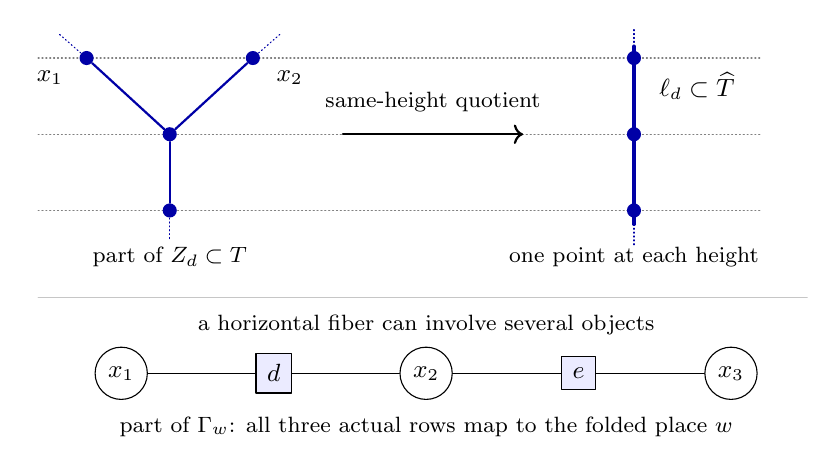
\begin{tikzpicture}[x=.88cm,y=.88cm,font=\small,
  every node/.style={align=center},line cap=round,line join=round,
  row/.style={draw,circle,fill=white,inner sep=3pt},
  object/.style={draw,rectangle,fill=blue!8,inner sep=4pt},
  dot/.style={circle,fill=blue!65!black,inner sep=1.8pt}]
  \draw[densely dotted,gray] (.4,-.15)--(10.85,-.15);
  \draw[densely dotted,gray] (.4,-1.25)--(10.85,-1.25);
  \draw[densely dotted,gray] (.4,-2.35)--(10.85,-2.35);
  \node[dot] (za) at (1.1,-.15) {};
  \node[dot] (zb) at (3.5,-.15) {};
  \node[dot] (zc) at (2.3,-1.25) {};
  \node[dot] (zd) at (2.3,-2.35) {};
  \draw[thick,blue!65!black] (za)--(zc)--(zb);
  \draw[thick,blue!65!black] (zc)--(zd);
  \draw[densely dotted,blue!65!black] (za)--(.7,.2);
  \draw[densely dotted,blue!65!black] (zb)--(3.9,.2);
  \draw[densely dotted,blue!65!black] (zd)--(2.3,-2.78);
  \node[anchor=east] at (.9,-.43) {$x_1$};
  \node[anchor=west] at (3.7,-.43) {$x_2$};
  \node[font=\footnotesize] at (2.3,-3.02) {part of $Z_d\subset T$};
  \draw[->,thick] (4.8,-1.25)--(7.4,-1.25);
  \node[fill=white,inner sep=2pt,font=\footnotesize] at (6.1,-.78)
    {same-height quotient};
  \draw[very thick,blue!65!black] (9,-2.55)--(9,.02);
  \draw[densely dotted,blue!65!black] (9,-2.55)--(9,-2.85);
  \draw[densely dotted,blue!65!black] (9,.02)--(9,.28);
  \node[dot] at (9,-.15) {};
  \node[dot] at (9,-1.25) {};
  \node[dot] at (9,-2.35) {};
  \node[anchor=west,fill=white,inner sep=2pt] at (9.28,-.55)
    {$\ell_d\subset\widehat T$};
  \node[font=\footnotesize] at (9,-3.02) {one point at each height};

  \draw[gray!45] (.4,-3.6)--(11.5,-3.6);
  \node[font=\footnotesize] at (6,-4.0)
    {a horizontal fiber can involve several objects};
  \node[row] (x1) at (1.6,-4.7) {$x_1$};
  \node[object] (d) at (3.8,-4.7) {$d$};
  \node[row] (x2) at (6,-4.7) {$x_2$};
  \node[object] (e) at (8.2,-4.7) {$e$};
  \node[row] (x3) at (10.4,-4.7) {$x_3$};
  \draw (x1)--(d)--(x2)--(e)--(x3);
  \node[font=\footnotesize] at (6,-5.47)
    {part of $\Gamma_w$: all three actual rows map to the folded place $w$};
\end{tikzpicture}
\caption{Strict folding is the transitive quotient generated by identifying
same-height points within each $Z_d$. The upper panel shows the image
of one subtree; horizontal guides indicate height. It does not identify
arbitrary equal-height points of $T$. The lower panel records how two
objects can make three actual rows equivalent at one height: an incidence
$x,d$ means $x\in Z_d$. Such incidence chains describe the horizontal
fiber $\Gamma_w$, whose stabilizer and homology are analyzed below.}
\label{fig:row-refinement-folding}
\end{figure}


\begin{lemma}[Raw horizontal jump vectors]\label{close:raw-jumps}
Fix an actual row group $X$ at a given level, and represent its actual
rows by frame cosets $pX\subset L$. A jump from $pX$ to $qX$ through
one object $d$ has a raw horizontal one-chain representative with
divergence $q-p$. Its coefficient support is contained both in a
finite union of $S_dr$ and in the union of the actual $X$-cosets
incident to $d$. Root-row representatives are taken before eliminating
the root relation.
\end{lemma}

\begin{proof}
The support assertion uses Theorem~\ref{coeff:support}. Fix an actual group \(X\) of the given level, using its one-chain generators in the horizontal Fox quotient of \(L\); rows now have frame cosets \(pX\) in \(L\). We use raw vectors on those generators, i.e. before eliminating the root relation if there is one. For any jump \(pX\to qX\) through \(d\), take \(1\ne a\in S_d\cap pXp^{-1}\), \(1\ne b\in S_d\cap qXq^{-1}\). The difference \(d(q)-d(p)\) (here the symbol on group elements denotes Fox chains) is represented by a raw vector obtained as
\[
 q\Delta_X(q^{-1}bq)-p\Delta_X(p^{-1}ap) -
       (\Delta(b)-\Delta(a)).
\]
For the last parenthesis use an expression by cycles from the \(M_x^d\) in the current level, with coefficients over \(D_{S_d}\), possible by the period isomorphism. In moving any such cycle from a conjugate row to its horizontal coordinates the frame chain terms cancel. In particular each may be written by differences of normalized elements just as in this formula, since such differences span the intrinsic cycle space modulo 2-boundaries for a nontrivial group. This proves the representation assertion by the conjugation rule. All coefficients are thus supported (in the sense of Theorem~\ref{coeff:support}) in finite unions of \(S_d r\), lying also within the union of actual \(X\)-cosets incident to \(d\). The divergence is literally \(q-p\).
\end{proof}

\subsection{The root-cylinder correction}

\begin{lemma}[Isolation and splitting of root cylinders]\label{close:root-cylinder}
Suppose the actual row is
\[
 X=B*_{\langle z\rangle=\langle u^a\rangle}\langle u\rangle,
 \qquad a>1,
\]
where $B$ is free and $z$ is root-indivisible in $B$. Put
$U=\langle u\rangle$, $\alpha=1+u+\cdots+u^{a-1}$, and
$R=\alpha\mathbf e_u-d_B(z)$. Let $V=\sum_iV_i$ be a finite sum of raw
vectors whose coefficients have the support patterns of
Lemma~\ref{close:raw-jumps}, for distinct members of a strict
quasiconvex system. If $V=PR$ in the division-field chain module
(necessarily $P=V_u\alpha^{-1}$), then, after applying the simultaneous
scalar-function map, $P$ is supported within a bounded neighborhood
of the corresponding finite union of peripheral neighborhoods.
It can be split among those neighborhoods outside a bounded set, so
that subtracting the corresponding multiples of $R$ makes each $V_i$
finitely supported without changing its divergence. The same
assertion holds after restriction to a specified actual $X$-coset.
\end{lemma}

\begin{proof}
The subgroup \(U\) is maximal cyclic in \(X\). Indeed, distinct edges at a
\(B\)-vertex of the root Bass--Serre tree have trivially intersecting
stabilizers, since \(z\) is root-indivisible in \(B\). Each nontrivial
\(u^m\) therefore has its own cyclic vertex as its only fixed vertex of
that type, with stabilizer \(U\).

The internal root relation generates the kernel of the row chain
quotient. Thus
\[
 V=P R,\qquad P=V_u\alpha^{-1},\qquad R=\alpha\,{\bf e}_u-d_B(z).
\]
After applying the simultaneous scalar-function map, \(P\) is supported
on \(U\)-cosets passing through a bounded neighborhood of the same
subgroups. Their union is quasiconvex, since it consists of finitely
many quasiconvex sets based at the identity. We show that \(P\) vanishes
far from this union, working within each specified actual \(X\)-coset.

Choose a ball radius
large enough to contain every translate used in the fixed words for
$u^a$ and $z$, and every right multiplication in $R$. If two
contributing periodic $U$-quasigeodesics meet such a ball far from the
quasiconvex union, thin quadrilaterals force them to fellow-travel for
a distance tending to infinity on their way back to that union.
Distinct cosets of the ambient maximal cyclic group have uniformly
bounded coarse overlap, so these quasigeodesics belong to the same
ambient cyclic coset. In a specified $X$-coset they are the same
$U$-coset: the intersection of the ambient maximal cyclic group with
$X$ is $U$, by maximality in $X$.

Write $p_n=P(lu^n)$ in this isolated cylinder. Where $V_u=0$, the
$u$-equation says that $a$ consecutive values sum to zero. Subtracting
two consecutive such equations gives $p_n=p_{n-a}$. The $B$-equations
can now be read on an oriented edge of the axis of $z$ in the free
Cayley tree of $B$. The sum of the translates of the based path
$d_B(z)$ has nonzero signed count on that edge; any initial or terminal
hairs cancel. Only coefficients with indices in the same
$\langle z\rangle$-coset contribute, and their indices lie in a fixed
finite interval. The local periodicity makes them equal, so this
nonzero integer multiple of $P(l)$ must vanish. Thus $P(l)=0$.

After this support bound, write $P=\sum_i P_i+P_0$, with $P_0$ finitely
supported and each $P_i$ supported in the separated tail near the
$i$th peripheral subgroup. Right multiplication by the finite
polynomial matrix $R$ enlarges supports by a fixed amount only. Since
$PR=\sum_iV_i$, each $V_i-P_iR$ vanishes outside a bounded set.
Moreover
\[
 \partial(P_iR)
 =P_i\bigl(\alpha(u-1)-(z-1)\bigr)=0.
\]
Consequently the correction preserves divergence. These are
operations on scalar functions after projection; no multiplicativity
of the scalar-function map for $\alpha^{-1}$ is asserted or needed.
Its right-group equivariance is precisely what preserves the
polynomial equations. Finally, all these right multiplications belong
to $X$, so they preserve each left $X$-coset and commute with
restriction to it.
\end{proof}

\subsection{The folded incidence trees}

\begin{lemma}[Tree structure and homology of a folded row]\label{close:folded-row}
For every folded place $w$, its incidence graph $\Gamma_w$ is a tree.
The $Y_w$-action is cocompact, with one orbit of actual row vertices;
its vertex groups are the indicated $X_x$ and $S_d$, and its incidence
groups are $M_x^d$. The inclusion induces an isomorphism
\[
 H_1(Y_w;D_L)\xrightarrow{\ \cong\ }H_1(L;D_L).
\]
\end{lemma}

\begin{proof}
Sum these raw vectors around a putative simple circuit, fixing one frame per visited \(x\). The sum is zero in the actual row chain quotient. Apply the simultaneous scalar function assertion, with all divergence and polynomial right products preserved. Outside bounded sets the supports of the various summands are disjoint, even in any fixed thickenings: they lie within bounded distance of the distinct \(D_d\), with trivial intersections. For free \(X\) the sum was zero literally, forcing finite function support for each vector. But finite chains in one actual \(X\)-coset cannot have total divergence \(1\) or \(-1\) there.

For a root row the raw sum around the circuit lies in the kernel of
the row chain quotient and therefore is $PR$ with
$P=V_u\alpha^{-1}$. Lemma~\ref{close:root-cylinder} corrects each
circuit summand by a divergence-zero function boundary and makes it
finitely supported. In any frame coset used at the end of a jump the
remaining divergence has total mass $1$ or $-1$. A finitely supported
one-chain in a Cayley graph has total divergence zero, giving the same
contradiction as in the free case.

The stabilizer and cocompactness assertions in the statement now follow by equivariance. The Bass--Serre Mayer--Vietoris sequence on \(\Gamma_w\) gives the homology assertion: edge \(H_0=0\) and the sum of edge \(H_1\)'s into the \(S_d\)-summands is exactly an isomorphism, leaving just the \(X\) inclusion.
\end{proof}

\begin{lemma}[Detection and separation at a folded level]\label{close:folded-separation}
Every noncyclic subgroup of $Y_w$ is detected in ambient height-kernel
homology. Stabilizers of two distinct folded places at the same level
intersect at most cyclically.
\end{lemma}

\begin{proof}
We verify detection: every noncyclic \(H\le Y_w\) has some \(\Delta(h)-\Delta(h')\) nonzero in ambient height-kernel homology. For an elliptic subgroup on \(\Gamma_w\) use the known \(S_d\) detection, or detection in \(X\). The latter is immediate in a free group by disjoint support away from bounded sets for normalized paths of two noncommensurable elements and divergence \(1\).

In a root group use its own cyclic Bass tree. Elliptic noncyclic subgroups are in a free base with independent columns. Otherwise choose two hyperbolics with axes in different components off a pivot \(B\)-node (neither axis through the pivot), taking that node as base by conjugation. Such separated axes exist: the tree action has trivial long-segment stabilizers, so a nonelliptic noncyclic subgroup has independent hyperbolics (an all-elliptic subgroup without a fixed point fixes tails towards an end; an end-fixing subgroup has trivial kernel of translation on tails); translate independent axes to separate them as far as needed.

Write normalized paths from the base to its translates by using cyclic-amalgam normal forms and substituting \(d_X(u)=\alpha^{-1}d_B(z)\). For each hyperbolic \(h\), support at the pivot \(B\)-coset comes only from finitely many powers' translates of the used pieces, staying within bounded distance of the one adjacent cyclic stabilizer towards the axis (plus finite sets). Indeed \(U\)-steps spread just in the \(B\)-cosets incident to that cyclic node, using finitely many \(U\)-coset translates; the translated tree paths go out and back along the axis with disjoint hairs to \(h^jB\).

The two incident cyclic stabilizers intersect trivially. Equality would force a function chain on that pivot coset with finite support and divergence of total mass one, impossible.

We next treat a subgroup that is nonelliptic on the folded incidence tree.
If \(H\) itself is nonelliptic and noncyclic on \(\Gamma_w\), similarly pick separated axes there off an \(X\)-node pivot (long segment stabilizers trivial by strictness). Conjugate to frame 1 there. Represent \(d(h)\) raw as above on the path through \(d\)-nodes to \(hX\), ending at frame \(h\). Normalize by \((h-1)^{-1}\). Restricting support to the pivot coset \(X\), only finitely many \(\langle h\rangle\)-translates contribute, namely jumps through a neighbor of the pivot, always the one \(d\) towards its axis. Thus pivot support stays near \(D_d\). The two normalized paths have distinct such \(d\)'s and divergence 1.

These are enclosing support patterns for sums/products, hence remain usable before any scalar function projection. In particular in the root case a further factor \(\alpha^{-1}\) on the right can hit the pivot coset only from inside that coset, and spreads pivot support just along \(U\)-cosets based near the corresponding \(D_d\). If equal modulo boundaries, in the root case their difference is \(P R\) as above, with \(P\)-support thus satisfying the isolated-cylinder claim inside the pivot. Splitting \(P\) there at infinity separates two disjoint tails, allowing correction of the normalized paths by \(R\) to finite function support there while retaining divergence.

This is impossible, in the free case directly so without correction.

Finally compare two distinct folded places.
For different components at this level, any common subgroup cycle has expressions in the level basis supported inside their respective actual frame cosets by these same path formulas (in an arbitrary starting frame \(p\) compute normalized jumps to \(h p\) and on normalization adjust by \(d(p)\), which cancels in differences; moves changing only the frame within one coset just use an actual \(X\)-word). Eliminating \(u\) does not leave those cosets. Disjoint support in Theorem~\ref{coeff:support} makes the cycle zero in ambient homology. Detection proves the asserted separation.
\end{proof}

\begin{proposition}[Folded slot structure and restriction]\label{close:folded-slot}
Fix a folded vertex $v$ and one slot of incident folded edges $f$.
Let $K_f$ be the image of the endpoint map
$\Gamma_f\to\Gamma_v$. Then $K_f$ is a $Y_f$-cocompact subtree, every
object vertex $d$ of $\Gamma_v$ occurs in exactly one such $K_f$ with
its full stabilizer, and any absent incidence has at most cyclic
stabilizer. For each $H\le Y_v$ the natural map
\begin{equation}\label{close:slot-injection}
 \bigoplus_{f\bmod H}H_1(H\cap Y_f;D_L)
             \longrightarrow H_1(H;D_L)
\end{equation}
is injective.
\end{proposition}

\begin{proof}
Map each \(\Gamma_f\to\Gamma_v\) by the endpoint map, fixing the \(d\) labels. Its image is a subtree \(K_f\) of finite quotient under \(Y_f\). Each \(d\) of \(\Gamma_v\) occurs in exactly one of these subtrees (on the chosen slot, by its line) with full stabilizer. An incidence \(x,d\) can be absent there only with \(M_x^d\) cyclic, by the local period equality. The \(f\)'s with \(x\in K_f\) form a single \(X_x\)-orbit. Moreover \(\widetilde F=X_x\cap Y_f\) there acts on the local tree of actual edges over \(x\) mapping to \(f\), connected by the \(d\)'s incident to these actual edges. This is connected: a simple path between such edges in \(\Gamma_f\) projects back to \(x\) and has no repeated \(d\), hence uses only jumps with that same \(x\) in \(\Gamma_v\). Its quotient is finite with one actual edge-node orbit (\(X_x\) is transitive on the unfurled slot, and a transporter here necessarily fixes \(f\); incident object types there are finite as before). Denote the edge group of the actual slot by \(E\); these actual edge-nodes now have groups \(E\) up to conjugation. There are other vertex groups \(M_x^d\) and gluing groups \(M_e^d\) for actual edges \(e\). Thus \(\widetilde F\) is finitely generated, and \(H_1(E)\to H_1(\widetilde F)\) is an isomorphism after extension by the local period equality and nonzero incidence stabilizers again.

If $X_x$ is free, the preceding isomorphism makes
$\widetilde F$ a rank-$k$ free quasiconvex subgroup. Its Fox columns
in $X_x$ are independent, using the already known injection
$H_1(E)\to H_1(X_x)$. Restricting the same induced modules to any
subgroup of $X_x$ and decomposing over its cosets therefore gives
the joint homology injection, exactly as in the actual slot rule
of Proposition~\ref{row:restriction}.

For a root row, write its root splitting in the chosen slot as
\[
 X_x=E*_{\langle z\rangle=\langle u^a\rangle}\langle u\rangle.
\]
The actual edges of this slot correspond to the $E$-nodes of the
root Bass--Serre tree. Suppose first that a nonzero power in a root
cyclic-node stabilizer belongs to some $S_d$. Root closure puts
that whole cyclic stabilizer in $S_d$. Every adjacent root edge
then has nontrivial stabilizer intersection with $S_d$, so all the
$E$-nodes incident to this cyclic node join through the same $d$.
By $X_x$-equivariance, the same holds at every cyclic node, with
its corresponding object label. Connectedness of the root tree
therefore joins all actual edges of the slot over $x$ into one
folded edge. In this case $\widetilde F=X_x$.

Suppose instead that no root power belongs to any $S_d$, and fix
$M=M_x^d$. Its stabilizers at root edges and cyclic nodes are
trivial. The local period equality says that the first homologies
of its $E$-node intersections sum isomorphically onto $H_1(M)$.
The tree sequence has no remaining degree-zero contribution.
Consequently, if an $E$-node intersection is nontrivial, there is
only one such vertex-group orbit and no additional free graph
factor: either a second nontrivial vertex group or a free factor
would contribute extra first homology through the degree-zero
edge terms. Thus $M$ is contained in that $E$-node stabilizer.
The fixed $E$-node is unique, since the intervening root edges have
trivial $M$-stabilizer.

If $M$ meets no $E$-node nontrivially, its root-tree action is free.
It is a nontrivial finitely generated free group, and the same
period equality gives $H_1(M)=0$. Hence it is cyclic and acts
hyperbolically on the root tree. Such an incidence meets no actual
edge of this slot and gives no identification of slot edges.
The other incidences meet exactly one actual edge, by the preceding
paragraph. Thus no object joins distinct actual edges in the
no-hit case, and $\widetilde F=E$ with its actual inclusion.

Both root alternatives give quasiconvexity and the needed comparison
after restriction to an arbitrary subgroup of $X_x$. When
$\widetilde F=X_x$, there is one folded-edge orbit over $x$ and the
comparison is the identity. When $\widetilde F=E$, folded edges
retain the actual $E$-cosets, and the actual-slot induced-module
injection of Proposition~\ref{row:restriction} applies to all their
intersection summands simultaneously. These are the vertex-node
comparisons used next.

Compare now the Bass--Serre Mayer--Vietoris sequence for \(H\) on \(\Gamma_v\) with the sum for \(H\cap Y_f\) on \(K_f\). At the \(d\)-vertices the summed rows map isomorphically, and likewise for incidence edge rows except for the absent ones, whose target stabilizers are at most cyclic (thus the \(H_1\) map on edge rows is onto, and the \(H_0\) map injects). At actual \(x\)-nodes the vertex \(H_1\) map injects by the just-proved subgroup-wise statement. Chasing the sequence gives exactly \eqref{close:slot-injection}: a putative kernel first has zero projected edge-\(H_0\) coordinate, so lifts to vertex \(H_1\); there subtract a lifted edge relation and use vertex injectivity.
\end{proof}

\begin{corollary}[Strict folded tree]\label{close:folding}
The quotient $\widehat T$ is a tree with one $L$-orbit at each level,
and every $Z_d$ maps onto a monotone line $\ell_d$. Its row groups and
slot maps have the conclusions of Lemmas~\ref{close:folded-row} and
\ref{close:folded-separation} and
Proposition~\ref{close:folded-slot}. Stabilizers of finite monotone
paths in any fixed height range inject jointly on first field
homology into $L$, over path-orbit representatives.
\end{corollary}

\begin{proof}
The quotient-tree and orbit assertions were proved in the construction.
Start the homology assertion at one folded edge, using
Lemma~\ref{close:folded-row}, and extend a path one edge at a time at
either endpoint. Apply \eqref{close:slot-injection} with $H$ equal to
the preceding path stabilizer. At every change of representative use
the inverse monomial coefficient shift, so that each summand has its
canonical ambient image. Iterating proves the asserted joint
injection.
\end{proof}

\section{Enlargement at shared line ends}\label{close:line-ends}

Distinct object stabilizers now intersect trivially, but their folded
lines may still share an end. We replace such groups by full end
stabilizers, prove that these remain quasiconvex and virtually compact
special, and show that a genuine enlargement strictly increases the
total injected homology dimension, which remains at most $k-1$. This
is the final step in constructing the terminal system.

\subsection{End kernels and tail homology}

\begin{lemma}[End stabilizers]\label{close:end-kernels}
Suppose two distinct folded lines share an end. Choose the positive
orientation if possible, reversing all orientations otherwise. The
set of distinct positive ends $\xi$ of the $\ell_d$ has finitely many
$G$-orbits. For $A_\xi=\Stab_G(\xi)$ and $S_\xi=A_\xi\cap L$, one has
$h(A_\xi)\ne0$, and $S_\xi$ is the increasing union of pointwise tail
stabilizers on any chosen line ending at $\xi$. Distinct $A_\xi$
intersect at most cyclically.
\end{lemma}

\begin{proof}
If some folded lines of distinct \(d\)'s share an end, choose a sign with this property, say positive (otherwise reverse orientations). Consider the system of \textbf{distinct} positive ends \(\xi\) of the \(\ell_d\)'s, with stabilizers \(A_\xi\) and kernels \(S_\xi\). These have finite orbit set, and height translators. \(S_\xi\) is the increasing union of pointwise tail stabilizers along any such line ending there (height-zero translates preserving the end fix tails since height on the line is monotone). Different \(A_\xi\)'s meet at most cyclically: a common element preserves the connecting geodesic, hence has height zero (height has a minimum along it), and fixes the line pointwise; use distinct same-level places there.
\end{proof}

\begin{lemma}[Joint injection for tails and ends]\label{close:tail-injection}
For representatives of the $L$-orbits of positive ends, the map
\[
 \bigoplus_\xi H_1(S_\xi;D_L)\longrightarrow H_1(L;D_L)
\]
is injective. The homology of every pointwise tail group $K$ also
injects into ambient homology and has finite dimension. In particular
$0<\beta(S_\xi)<\infty$.
\end{lemma}

\begin{proof}
Choose rays to representatives of the $L$-orbits of ends, starting at
one common folded edge level $w$ whose actual rows are free. For
each ray let $K$ be its pointwise stabilizer, and let $K_n$ stabilize
its length-$n$ prefix, so $K_n\downarrow K$. We show that every
finite-dimensional test space in the sum of these tail homologies
injects into the sum for sufficiently long finite prefixes. Folded
path inertia will then give its ambient injection. This finite-test
argument is needed because the groups here form decreasing
intersections.

Work on the fixed incidence tree $\Gamma_w$. At an object node $d$,
a prefix stabilizer intersects $S_d$ in the full group while the
prefix lies on $\ell_d$, and at most cyclically after it leaves that
line. These actual intersections stabilize for each fixed $d$.
To see this, consider a nontrivial cyclic intersection after departure.
At an off-line place, a nonzero element of $S_d$ fixing that place
acts hyperbolically on its incidence tree: strictness forbids a fixed
other object node, and enlargement of $Z_d$ forbids a fixed actual
row. If a power fixes a continuation $f$, its axis lies in $K_f$.
The translate of $K_f$ by the cyclic generator contains the same axis.
But distinct $K_f$ in one slot have no common object node, whereas
that axis passes through object nodes. Hence the generator already
fixes the continuation. There is no proper finite-index drop; a drop
to the trivial group is permanent. The same reasoning gives
stabilization at each fixed incidence edge.

In the Bass--Serre sequence for $K$ on $\Gamma_w$, the incidence
$H_1$ terms sum isomorphically onto the object-node terms: use the
period rule at full nodes, and vanishing of cyclic first homology at
the others. The remaining sequence has the actual-row homologies as
an injected subspace, with quotient injecting into the incidence
$H_0$ terms. Fix a finite-dimensional test space and finite cycle
representatives. First consider their finitely supported $H_0$
projections. All their used incidence stabilizers have stabilized
for large $n$. A transporter identifying two specified incidence
lifts while matching length-$n$ prefixes lies in a nested coset of
one of these stabilizers. Once that stabilizer is fixed, persistent
nonempty cosets coincide and identify the whole rays. Thus no new
identification of the finite $H_0$ data remains for all large $n$,
even when prefix orbits initially merge.

For the remaining actual-row part, use the free Cayley tree of each
$X_x$ in its actual frame. Represent the finitely many needed cycles
inside finite connected subgraphs of the quotients by $K\cap X_x$.
These subgraphs embed jointly and disjointly in the corresponding
quotients for $K_n$ once $n$ is large. Indeed a proposed identification
between two chosen regular frame vertices has a unique possible
transporter. If it matched every prefix it would match the full
rays, so each unwanted identification disappears at a finite stage.
There are only finitely many pairs to test. Disjoint connected
subgraphs of a graph give simultaneous free factors up to their
basepoint conjugations, and hence joint first-homology injection,
also after extension to $D_L$.

The tree sequences now give injection on the original finite test
space into the finite-prefix homologies. Those inject jointly into
$H_1(L;D_L)$ by Corollary~\ref{close:folding}. This proves both the
individual tail assertion and the joint assertion after taking the
increasing union over ray starting levels. That union is $S_\xi$.
The ambient dimension is $k-1$, so all these dimensions are finite.
Finally $S_\xi$ contains the kernel of an old line ending there; the
just-proved injection preserves its positive homology.
\end{proof}

\subsection{Simultaneous boundary factors on a tail}

\begin{proposition}[The tail free-product decomposition]\label{close:tail-splitting}
Let $K$ be the pointwise stabilizer of a positive ray contained in an
old line, starting at an actual free-edge level $w$. An object vertex of $\Gamma_w$ is called full if
its line contains that entire tail. There are finitely many $K$-orbits
of full vertices. With representatives $d_1,\ldots,d_m$, one has
\begin{equation}\label{close:tail-product}
 K\cong\Bigl(*_{j=1}^m S_{d_j}\Bigr)*F_r,
 \qquad r<\infty.
\end{equation}
The displayed embeddings of full factors are their actual subgroup
embeddings, up to the usual independent choices of conjugating
basepoint paths.
\end{proposition}

\begin{proof}
Call an object node of $\Gamma_w$ full when its line contains the
whole tail. At such a node the $K$-stabilizer is $S_d$. Each full
node meets a noncyclic actual-row stabilizer, by its positive beta
and the period rule. The actual-row homologies inject in the tree
sequence used above. Thus there are finitely many $K$-orbits of
noncyclic $K_x=K\cap X_x$, and each is a finite-rank free group.
Quasiconvex double-coset finiteness inside $X_x$ gives finitely many
nontrivial incidence orbits at each. Consequently there are finitely
many full-node orbits.

Remove the full nodes, and let $B$ stabilize one of the remaining
components. The sum of the boundary-incidence homologies is an
isomorphism onto the removed full-node homologies. The tree sequence
therefore bounds $\beta(B)$ by $\beta(K)$. We also need finite
generation of $B$. Its remaining object-node stabilizers are cyclic
or trivial. At a cyclic actual-row stabilizer, strictness and root
closure imply that any nontrivial incident intersection is the whole
stabilizer and occurs on at most one edge. Collapse these redundant
cyclic-row leaves. Noncyclic actual-row stabilizers and their
nontrivial incident edges have finite orbit lists as above; hence
every remaining component of nontrivially stabilized edges has
finitely generated stabilizer and finite core, or is a single cyclic
group. The leftover trivial edges give a free product. Its
free-product dimension formula and $\beta(B)<\infty$ leave only
finitely many nontrivial factors and finite free rank. Thus $B$ is
finitely generated.

We claim that the boundary incidence groups at this component are
\emph{simultaneous} free factors of $B$. Choose an actual base vertex
and take the paths to its translates by a finite generating set of
$B$, together with all their $B$-translates. Their connected union
$U\subset T$ is $B$-invariant and has bounded height range because
$B\le L$. Choose an actual free-edge level $w'$ on the tail above
that range by more than the actual capture length.

For an actual row $y$ over $w'$, the group $B_y=B\cap X_y$ fixes
$y$ and preserves $U$, hence fixes the bridge from $y$ to $U$.
If $B_y$ is noncyclic, the noncyclic ambient bridge stabilizer is
captured in one $S_{d'}$, so $B_y\le S_{d'}$ and $y\in Z_{d'}$.
If $B_y$ is cyclic and meets an incident $S_{d'}$ nontrivially,
root closure again puts all of $B_y$ there. Strictness makes the
object unique. Thus all nontrivial incidences in the $B$-action on
$\Gamma_{w'}$ form stars centered at objects, with redundant
actual-row leaves. Collapsing those stars leaves trivial edge
groups. Any remaining actual-row stabilizers are cyclic and
contribute free factors of rank one.

Identify the surviving object groups in the original $\Gamma_w$.
If $B\cap S_{d'}$ is noncyclic, it fixes both the selected tail
place and the place of $\ell_{d'}$ at every original tail level.
Same-level separation forces these places to agree, so $d'$ was
already full at the starting level. For any full $d'$, an element
of $B\cap S_{d'}$ fixes $d'$ and preserves the original component
of $B$. If the connecting path crosses another full node, strictness
makes this intersection trivial. Otherwise $d'$ neighbors that
component, and its intersection is precisely the unique boundary
incidence stabilizer $M_x^{d'}$. This is free, being a subgroup of
the free row $X_x$. Other surviving object groups are at most cyclic.

Every original boundary incidence is retained in this argument,
including cyclic ones. Its actual object label $d'$ is the same at
$w$ and $w'$. Two such labels become $B$-equivalent at the higher
level exactly when they were already $B$-equivalent originally.
The trivial-edge splitting just constructed therefore makes $B$
free, with the entire original boundary family as simultaneous free
factors, up to independent basepoint conjugations.

Return to the splitting of $K$ obtained by removing the full nodes.
Substitute these simultaneous factors for the boundary attachments
on the $B$-sides of its Bass presentation. This eliminates each
boundary factor against its image in the corresponding $S_d$ and
gives, with the actual embeddings,
\[
 K\cong\Bigl(*_{j=1}^m S_{d_j}\Bigr)*F_r.
\]
The trivial-edge $H_0$ terms give
\begin{equation}\label{close:free-product-budget}
 \beta(K)=\sum_{j=1}^m\beta(S_{d_j})+(m-1)+r.
\end{equation}
Here $m\ge1$, since the tail was chosen on an old line. Positive
beta for the full factors and finite $\beta(K)$ give finite $m,r$.
A cyclic free factor contributes one through $r$; it is not lost
through its zero intrinsic first field homology.
\end{proof}

\subsection{Virtually free ascending quotients}

Filling the full factors in the tail decomposition
\eqref{close:tail-product} produces a finitely generated virtually free
base. The induced ascending map may fail to be injective. We first
remove this obstruction so that the ascending-torus theorem can be
applied to the filled end groups.

\begin{lemma}[Stabilizing a virtually free endomorphism]\label{close:virtually-free-endo}
Let $V$ be a finitely generated virtually free group and
$\phi:V\to V$ an endomorphism. The sequence $\ker\phi^n$ is eventually
stationary. Its ascending torus is therefore isomorphic to the
ascending torus of an injective endomorphism of a finitely generated
virtually free group. In the injective case this torus has a
finite-index subgroup that is an ascending torus of an injection of a
finite-rank free group.
\end{lemma}

\begin{proof}
Choose a finite quotient $q:V\to Q$ with torsion-free kernel, and put
\[
 F=\bigcap_{\psi:V\to Q}\ker\psi.
\]
There are finitely many such maps because $V$ is finitely generated.
Thus $F$ is a fully invariant finite-index normal subgroup contained
in $\ker q$. It is torsion-free and virtually free, hence free of
finite rank. The ranks of the free groups $\phi^n(F)$ form a
nonincreasing sequence and eventually agree. For all sufficiently
large $n$, the surjection
$\phi:\phi^n(F)\to\phi^{n+1}(F)$ is consequently an isomorphism by
Hopficity of finite-rank free groups. Hence the iterated kernels
stabilize on $F$. They stabilize on all of $V$ as well: once their
intersections with $F$ agree, the increasing kernels have a bounded
finite quotient modulo that common intersection, bounded by $[V:F]$.

If $N=\ker\phi^n$ is the stable kernel, then
$V/N\cong\phi^n(V)$ and the induced endomorphism is injective. In the
ascending torus every element of $N$ is already trivial, by iterating
the stable-letter relation. Thus replacing $V$ by $V/N$ leaves that
torus unchanged.

Now suppose $\phi$ is injective. Choose a fully invariant finite-index
normal free subgroup $F_0\le V$ as above and replace it by
\[
 F_\infty=\bigcup_{j\ge0}\phi^{-j}(F_0).
\]
The terms increase, are normal, and have index at most $[V:F_0]$, so
the union equals one of them. It is torsion-free by injectivity and
therefore free of finite rank. Moreover
$\phi^{-1}(F_\infty)=F_\infty$ and
$\phi(F_\infty)\le F_\infty$. The induced endomorphism of the finite
group $V/F_\infty$ is injective and hence an automorphism. Choose a
positive power for which this finite action is trivial. Ascending
normal forms then show that the subgroup generated by $F_\infty$ and
the corresponding stable-letter power has finite index and is the
ascending torus of the induced injection on $F_\infty$.
\end{proof}

\begin{proposition}[Quasiconvex and virtually compact special end groups]\label{close:end-vcs}
Each end stabilizer $A_\xi$ is finitely generated, quasiconvex in $G$,
field-acyclic, and virtually compact special. It is torsion-free,
locally indicable, coherent, of type $F$, and of cohomological
dimension at most two.
\end{proposition}

\begin{proof}
Choose $\sigma$ in the group of the original line with positive
height $p$, and put $A_\xi'=A_\xi\cap h^{-1}(p\mathbb Z)$.
If $K$ stabilizes a starting tail on that line, then
$S_\xi=\bigcup_{n\ge0}\sigma^nK\sigma^{-n}$. Thus $A_\xi'$ is
the ascending torus with base $K$ and injection given by conjugation
by $\sigma^{-1}$. The tail decomposition expresses $K$ as finitely
many full factors $S_{d_j}$ and a finite-rank free group. Each
$S_{d_j}$ lies in the finitely generated group $D_{d_j}\cap A_\xi'$,
which has finite index in $D_{d_j}$. These finitely many groups,
the free generators, and $\sigma$ generate $A_\xi'$. Therefore
$A_\xi$ is finitely generated.

Its height kernel has positive finite beta by tail injection, so the
period rule and its actual-tree gate criterion make $A_\xi$
quasiconvex in $G$. The ambient injective Fox two-boundary remains
injective in subgroup-induced coefficients, giving $H_2=0$ over
its division field. The cyclic height sequence gives the remaining
field acyclicity: on finite-dimensional kernel homology,
translation minus identity becomes invertible over the skew Laurent
division extension, by its leading degree. Torsion-freeness, local
indicability, coherence, and cohomological dimension at most two
are inherited from $G$. Quasiconvexity supplies a finite classifying
space \cite[Theorem~5]{MeintrupSchick2002}.

It remains to prove VCS. In $A_\xi'$ take the peripheral occurrences
$D_d\cap A_\xi'$ for lines ending at $\xi$. They form a strictly
malnormal family of quasiconvex VCS groups. Every such occurrence
can be moved, by a power of $\sigma$, to a full factor at the chosen
starting tail, so there are finitely many conjugacy types. If one
peripheral is all of $A_\xi'$, VCS is already known. Otherwise this
is a proper relatively hyperbolic pair.

For each representative peripheral, choose a finite-index normal
subgroup avoiding any prescribed finite set, and kill its
intersection with $S_d$. Residual finiteness of the whole VCS
peripheral permits these choices. The kernels are normal,
height-zero, and equivariant on all conjugate occurrences. The
peripheral images are finite-by-infinite-cyclic, so sufficiently
deep relative filling gives a hyperbolic quotient
\cite{Osin2007}.

The actual tail free-product decomposition identifies its filled
base as
\[
 V=\Bigl(*_{j=1}^m S_{d_j}/N_{d_j}\Bigr)*F_r,
\]
a finitely generated virtually free group. Conjugation by
$\sigma^{-1}$ takes each full line to another full line: its
translated starting ray contains the original starting ray.
Equivariance therefore takes its selected kernel into that of the
corresponding factor. This supplies an endomorphism of $V$.
All peripheral occurrences are reached by moving a sufficiently
late full tail back to the starting level. Hence the entire filled
quotient of $A_\xi'$ is exactly the ascending torus presentation
of that endomorphism; injectivity of the endomorphism is not assumed.

Lemma~\ref{close:virtually-free-endo} replaces this presentation by
an injective virtually free ascending torus and then gives a
finite-index free ascending torus. It is hyperbolic, so
Theorem~\ref{asc:vcs} makes the filled group VCS. We have obtained
arbitrarily deep such fillings, with hyperbolic VCS peripheral
images. Together with the finiteness and field hypotheses proved
above, these are precisely the inputs to
Theorem~\ref{fill:criterion}. Thus $A_\xi'$, and hence $A_\xi$, is VCS.
\end{proof}

\subsection{Termination of both closure operations}

\begin{proposition}[Strict growth at a shared end]\label{close:end-growth}
Replacing the objects by distinct end stabilizers preserves all
admissibility conditions. If some two distinct old lines share an end
in the chosen orientation, this replacement strictly increases the
budget. Subsequent cyclic closure does not decrease it.
\end{proposition}

\begin{proof}
Tail injection gives the new joint homology injection. To check
detection, choose a finitely generated noncyclic subgroup of any
noncyclic subgroup of $S_\xi$. It lies in one sufficiently late
tail group $K$. The free-product decomposition of $K$ detects it,
either in an old full factor or by the trivial-edge free-product
argument used in Lemma~\ref{close:join-detection}. Tail injection
preserves that nonzero cycle in $L$. Each new kernel contains its
constituent old kernels, so actual noncyclic path stabilizers remain
captured. The end-group and intersection lemmas supply the other
admissibility conditions.

Fix a new end $\xi$. Old $L$-orbits over its $L$-orbit correspond
exactly to $S_\xi$-orbits of old objects ending there. Their finite
list of representatives is simultaneously full on a sufficiently
late tail. If there are $m$ such representatives, the tail
free-product formula and tail injection give
\[
 \beta(S_\xi)\ge
   \sum_{j=1}^m\beta(S_{d_j})+(m-1).
\]
This is strictly greater than the old sum when $m\ge2$.

Suppose $m=1$ and equality holds. Every later tail on the chosen
original line contains its actual full factor $S_d$. Equality in
\eqref{close:free-product-budget} forces that tail group to have
exactly this one full factor and no free part; hence it is $S_d$
with its actual inclusion. Their increasing union gives
$S_\xi=S_d$. Any second old object sharing this end would have its
nontrivial kernel inside $S_d$, contradicting strictness. Thus a
shared end forces strict growth even when the old objects belong
to one $S_\xi$-orbit.

Sum over the new $L$-orbits. The budget increases by a positive
integer whenever an end is genuinely shared. Cyclic closure then
restores strictness without decreasing the budget, and allows a new
folding on the same actual tree $T$. Testing both orientations at
each strict state therefore terminates within the bound $k-1$.
\end{proof}

\begin{theorem}[Terminal periodic system]\label{close:terminal-system}
Starting with the system of Proposition~\ref{gate:capture}, finitely
many cyclic-closure and end-enlargement rounds produce an admissible
strict malnormal quasiconvex virtually compact special system
$\{D_d\}$, with $S_d=D_d\cap L$, and a folded tree $\widehat T$ having
all the conclusions of Corollary~\ref{close:folding}. The associated
monotone lines $\ell_d$ of distinct objects share no end. Actual long
noncyclic path stabilizers remain captured, the kernels still detect
all noncyclic subgroups, and their joint homology budget is at most
$k-1$.
\end{theorem}

\begin{proof}
Use Proposition~\ref{close:strict-system} to reach a strict state.
Whenever an end is shared, apply the preceding construction in the
relevant orientation, then restore strictness and fold again. All
foldings use the same actual tree $T$. Test both orientations each
time strictness is restored. Proposition~\ref{close:end-growth} gives
a positive integral increase at every end-enlargement round, whereas
all budgets are at most $k-1$. There are consequently only finitely
many such rounds, and each intervening cyclic closure is finite.
The terminal state has exactly the asserted properties.
\end{proof}

\section{Relative geometry of terminal rows}\label{sec:07-transfer}

The terminal folding gives row groups assembled from actual rows and
height kernels. We first control their peripheral incidences and build
their relative geometry. The resulting comparison and intersection
lemmas will supply the finite-window hypotheses for the terminal path
argument, before any filling is chosen.

\subsection{Standing terminal data}

We work with the terminal system supplied by Theorem~\ref{close:terminal-system}. We retain the actual tree \(T\), the folded tree \(\widehat T\), the height homomorphism \(h:G\to\mathbb Z\), and \(L=\ker h\). An \emph{object} is an actual label \(d\), not merely a conjugacy class of subgroups. Its periodic group is \(D_d\), its height kernel is \(S_d=D_d\cap L\), its actual subtree is \(Z_d\), and its monotone folded line is \(\ell_d\). The following previously established features will be used explicitly.
\begin{enumerate}[label=(\roman*)]
\item The groups \(D_d\) form an equivariant malnormal system with finitely many orbits of quasiconvex virtually compact special subgroups. Distinct actual objects have trivial stabilizer intersection, and no two distinct lines \(\ell_d\) share an end. In particular the relevant cyclic intersections are root-closed in their row groups.
\item At a folded place \(w\), the fiber \(\Gamma_w\) is a bipartite tree with actual-row nodes \(x\) and object nodes \(d\). Their stabilizers are \(X_x\) and \(S_d\), and an incidence has stabilizer \(M_x^d\). Endpoint maps send an adjacent edge fiber onto the invariant subtree \(K_f\subset\Gamma_v\). On each slot an object node belongs to exactly one such image. All local data have finite quotient, and the actual intersections \(\widetilde F_{x,f}=X_x\cap Y_f\) are finitely generated and quasiconvex in \(X_x\).
\item There is a fixed actual capture length: the stabilizer of a sufficiently long actual segment, if noncyclic, lies wholly in one of the \(S_d\). The enlarged \(Z_d\)'s contain every actual incidence with nontrivial intersection. The cyclic dictionary, the reversal bound, and folded homology inertia are available.
\item For the relative free-product trees constructed below we use the expansion and phase-uniqueness conclusions of the expansion-gate argument, with their finite-window hypotheses. We will verify those hypotheses before invoking those conclusions.
\end{enumerate}
Throughout this section a \emph{nonparabolic} subgroup means a nontrivial subgroup not contained in any actual \(S_d\). A folded place means either a vertex or an edge; its stabilizer is denoted \(Y_w\).

\begin{lemma}[Capture of a fixed monotone ray]\label{transfer:ray-capture}
If \(1\ne c\in L\) fixes a monotone ray of \(\widehat T\) pointwise, then its end is an end of exactly one object line \(\ell_d\), and \(c\in S_d\).
\end{lemma}
\begin{proof}
Take a remote infinite subray $W$, high in the positive orientation
or low in the negative one. Over $W$ form the mapping cylinders of
the place trees $\Gamma$ and their endpoint maps. This is a simply
connected tree of contractible spaces. Its actual vertical pieces
are the connected components of the actual preimage of $W$; its
object vertical pieces are the intervals $\ell_d\cap W$. Construct
a bipartite graph with these pieces as vertices and one edge for
each incidence between them.

This incidence graph is a tree. There is a map from the cylinder
complex to the graph: actual continuations and object intervals
collapse to their vertex labels, place incidences map to the
corresponding edges, and incidence strips have the same two labels
at successive levels. Each prescribed vertex piece is connected.
Thus a graph circuit could be lifted, using connecting paths inside
these pieces, to a loop in the cylinder complex. Its image would be
that circuit, contradicting simple connectivity.

The element $c$ acts on this auxiliary tree. Every single-place
image is connected and $c$-invariant. If $c$ acted hyperbolically,
its axis would lie in every such image. The axis passes through
several object vertices, whose lines would consequently all contain
$W$, contrary to the absence of shared line ends. Hence $c$ fixes
a vertex of the auxiliary tree.

A fixed object vertex gives $c\in S_d$ immediately. If an actual
component is fixed, compare it with a bounded-height invariant
subtree of actual $T$ for $\langle c\rangle$, obtained from one
generator path and its translates. For remote $W$ these subtrees
are disjoint and their long connecting bridge is fixed pointwise.
The cyclic dictionary forces a capture-length subblock on that
bridge to have noncyclic ambient stabilizer. Capture puts $c$ in
some $S_d$, and the fixed actual endpoint over $W$ belongs to $Z_d$.
Thus $\ell_d$ meets $W$ in either case. Strictness makes this same
$d$ unique as $W$ recedes, so its line has the given end and
$c\in S_d$.
\end{proof}

\begin{lemma}[Bounded peripheral incidences]\label{transfer:bounded-incidence}
There is a uniform constant \(C\) such that \(Y_w\cap S_d\ne1\) implies \(d_{\widehat T}(w,\ell_d)\le C\). There are finitely many orbits of these incidences. If \(w\notin\ell_d\), the intersection is cyclic.
\end{lemma}
\begin{proof}
Suppose $Y_w\cap S_d\ne1$, and follow the path from $\ell_d$ to
$w$. At its departure vertex $v$, let $f$ be the first edge off the
line. The nontrivial intersection fixes $d$ in $\Gamma_v$ and its
nearest point in $K_f$. These are adjacent: an intervening object
node would contradict strictness. At their actual-row node $x$,
\[
 S_d\cap Y_f=M_x^d\cap\widetilde F_{x,f}.
\]
This intersection is cyclic. Local cocompactness and quasiconvex
double-coset finiteness in $X_x$ give finitely many departure types
$(d,v,f)$ with nontrivial intersection.

At every later off-line vertex, a nonzero element of this cyclic
group acts hyperbolically on the incidence tree. Its axis determines
at most one preserved continuation in each slot. Moreover a cyclic
generator fixing the vertex fixes a continuation whenever a nonzero
power does, by the stabilization argument in
Lemma~\ref{close:tail-injection}. Thus the path cannot reverse slots
after departure. Unbounded distance for one of the finitely many
departure types would give an off-line monotone ray fixed by a common
nonzero power. Lemma~\ref{transfer:ray-capture} would put its end on
$\ell_d$, which is impossible for a ray that has left that line in
a tree. This gives the uniform distance bound. The same finite
departure lists and unique continuations give finitely many
incidence orbits within that bound.
\end{proof}

\subsection{The unfilled relative models}

We now use these bounded incidence lists to construct the unfilled relative rows. The acting groups on adjacent places of \(\widehat T\) are denoted \(Y_f\le Y_v\), with conjugations implicit. Peripheral intersections mean all nontrivial \(Y_z\cap S_d\), up to \(Y_z\); include also the intersections with the extra maximal cyclics when those are added. Recall the hypotheses reached for these arguments: finite intersection orbit lists; included \(S_d\)'s (line through the place) full, others cyclic; malnormality; the incidence tree \(\Gamma_v\) with quasiconvex \(M_x\) at its actual \(X\)-pieces, and adjacent image subtree \(K_f\subset\Gamma_v\) of finite quotient, on which the \(S_d\)-nodes again have full groups and the \(X\)-intersections \(\widetilde F_x\) are finitely generated and quasiconvex in \(X_x\). All groups here are torsion-free before filling.

\begin{definition}[Exact relative embedding]\label{transfer:relative-embedding}
Let \(J\) be hyperbolic relative to a finite list \(\mathcal P\). An \emph{exact relative embedding} of \(B\le J\) means that:
\begin{enumerate}[label=(\roman*)]
\item the nontrivial groups \(B\cap pPp^{-1}\), for \(P\in\mathcal P\), have a finite list of representatives up to \(B\)-conjugacy;
\item \(B\) is finitely generated relative to this list; and
\item its coned Cayley graph maps quasi-isometrically into the coned Cayley graph of \(J\), with each peripheral apex sent to the corresponding actual peripheral coset.
\end{enumerate}
Thus the apex map is injective on actual cosets. ``Exact'' refers to these induced intersections; it does not require that an induced subgroup equal the ambient peripheral.
\end{definition}

\begin{lemma}[Relative row geometry]\label{transfer:relative-rows}
Under the local hypotheses just listed, each folded vertex row \(Y_v\) is hyperbolic relative to its finite induced peripheral system, and each adjacent edge map \(Y_f\hookrightarrow Y_v\) is an exact relative embedding. The assertions remain valid after adjoining the external maximal cyclic intersections, provided their incidence lists satisfy the same local hypotheses.
\end{lemma}
\begin{proof}
Each \(Y_v\) is hyperbolic relative first to just its included \(S_d\)'s: glue coned fine hyperbolic graphs for its actual \(X\)-nodes along the single apex points corresponding to their \(S_d\)-neighbors. In \(X\) these use the nontrivial malnormal quasiconvex incidence groups. This is a tree of graphs glued at points by \(\Gamma_v\); hyperbolicity and fineness follow piecewise, with finite edge orbit set and finite edge stabilizers.

The infinite vertex stabilizers of this glued graph are exactly the
included object groups, in their actual coset positions; ordinary
vertices have finite stabilizers. Thus
\cite[Proposition~3.47]{GerasimovPotyagailo2015} gives a finite relative
presentation with linear relative Dehn function. This comparison
requires neither absolute finite generation of $Y_v$ nor finite
generation of an $S_d$. The same comparison applies to the edge-row
model below with its exact induced apex stabilizers. A row equal to
a single peripheral has the degenerate relative presentation with no
ordinary generators or relators; a trivial row is immediate.

The edge group \(Y_f\) is relatively hyperbolic and cone-quasi-isometrically embedded with its induced peripheral structure for this list. Indeed use \(K_f\), gluing the corresponding relative models of \(\widetilde F_x\) (with all nontrivial intersections with incident \(M\)'s) at the included points. A nontrivial \(S_d\)-intersection for \(d\in\Gamma_v-K_f\) is witnessed adjacent to \(K_f\), in the corresponding actual piece (project from \(d\) to \(K_f\), using strictness).

The models at \(X\) embed relatively quasi-isometrically by ordinary quasiconvexity of \(\widetilde F_x\). One proof uses coarse nearest projection onto this quasiconvex orbit in \(X\): projections of an incident \(M\)-coset have bounded diameter if the coset stays far away, otherwise lie boundedly near an orbit of the exact intersection. This follows by thin quadrilaterals and quasiconvexity, then ordinary properness (normalize a close pair, and pairs at bounded distance have only finitely many orbits under the intersection). Thus projections coarsely bound every cone jump in the induced cone metric. The intersection system itself is malnormal and quasiconvex there, finite up to the subgroup.

Summing distances over the point gluings preserves the relative embedding (each internal passage between distinct gluing apices costs positively). These models are equivalent to relative Cayley metrics by relative cocompactness or normal paths along the Bass tree.

External cyclic peripheral intersections to be added in \(Y_v\) are maximal loxodromic cyclics there, disjointly malnormal. Indeed root-closedness and disjointness are inherited (including for the extra family), these groups meet no included conjugate nontrivially, and loxodromic elementary closures are virtually cyclic, hence cyclic here.

Thus adding them still gives relative hyperbolicity by elementary-subgroup peripheral enlargement~\cite[Corollary~1.7]{OsinElementary2006}. For finitely many additions, iterate this statement over the distinct maximal cyclic types: a remaining type cannot become conjugate into an earlier one without being commensurable with it. The relative embedding above persists with the induced intersections, as we now prove separately.

Use coned Cayley graphs (ordinary \(T\)-edges for finite relative generators, radial edges to coset apices). An embedded subgroup's cone path is mapped with fixed representative offsets \(p_\alpha\) for its peripheral list \(B\cap p_\alpha P_i p_\alpha^{-1}\), via \(b,bp_\alpha,bp_\alpha P_i\) at a jump. We can enlarge \(T\) by all offsets and ordinary letters needed, and also by a generator for each new loxodromic cyclic subgroup, whose translates now have uniform ordinary-edged quasigeodesic axis paths in the old coned graph. Embedded geodesics map to uniform quasigeodesics with no repeated old apices (actual apex map injective).

Recall the proper angle property at an old apex: for two incident ordinary vertices joined avoiding that apex in bounded length, the displacement belongs to a finite list inside the corresponding peripheral.

Project a new cyclic coset coarsely to the quasiconvex embedded orbit of \(B\) in this old graph. If two projections are far apart in the old metric, a \(B\)-comparison quasigeodesic between them, except for bounded ends, stays boundedly near that axis (coarse projection and thin quadrilaterals).

Frame vertices \(b\) sufficiently inside this portion are in fact at finite-list ordinary displacement from axis frame points \(a\). Indeed nearby apex turns on the comparison path have bounded angle: bypass via two short bridges to the axis a sufficiently large fixed distance before and after, avoiding the apex by quasigeodesicity, and the bounded axis subpath. The short bridge at \(b\) itself then has bounded angles at each jump, using one farther such bridge for a bypass and replacing occurrences of that apex along the comparison path by the bounded-angle detour. Take bridges geodesic so do not revisit the apex.

Proper angles give \(b^{-1}a\) from a fixed finite list. Pairs with a given displacement form one orbit under the coset stabilizer in \(B\). Normalizing one pair shows there are finitely many coset types with this large projection, and all such middle projections are at bounded relative distance of one another after coning the stabilizer if nontrivial (otherwise already bounded; finitely many pair orbits in the normalized types). End errors are bounded too by the old relative embedding.

Conversely every infinite cyclic intersection gives unbounded old projection. This gives exactly the finite induced new list (malnormal loxodromic cyclic subgroups also in \(B\), by the old embedding), and the nearest projection now bounds each additional shortcut in the enlarged metric of \(B\). Hence the assertions on relative hyperbolicity and embedding. Apply with \(B=Y_f\). All these constructions use only finite orbit lists. "Full" relative maps of peripheral groups are not required.

\end{proof}

\begin{lemma}[Hyperbolicity of the partial metric]\label{transfer:partial-hyperbolicity}
The tree of relative row spaces before filling is hyperbolic. Its metric is quasi-isometric to the partial Cayley metric on \(G\) obtained by allowing arbitrary \(S_d\)-moves and, if present, arbitrary moves in the additional root cyclics.
\end{lemma}
\begin{proof}
Spelling paths in the Bass presentation identifies the tree of
relative row spaces, up to quasi-isometry, with the partial Cayley
metric that permits arbitrary moves in the $S_d$ for the finitely
many $G$-orbit representatives. There are finitely many attaching
frames and offsets, every local cone uses one such group, and each
$S_d$ is fully available on its line. The additional cyclic groups,
if present, are fully available at their fixed places.

Use a finite linear relative presentation of $G$ relative to the
$D_d$ and any additional cyclics. Inside $D_d$, the partial metric
has bounded height fibers and is quasi-isometric to $D_d/S_d$, a
line; inside an added cyclic it is bounded. A partial-metric loop
therefore admits a relative filling with linearly many ordinary
relative cells. Their peripheral labels belong to fixed finite
lists, while the loop's own peripheral moves have bounded partial
length. The total partial length on peripheral cluster boundaries
is consequently linear in the original loop length.

Choose the filling with minimal ordinary relative area. A hole in
a peripheral cluster can be filled entirely in that peripheral,
by peripheral injectivity; doing so eliminates any ordinary cells
inside. We may therefore treat clusters as discs. Each cluster
boundary has a linear filling at a fixed Rips scale in its partial
metric: push vertices by bounded moves to a lifted height line and
fill there, or use the bounded metric for an extra cyclic. Combining
these fillings gives a linear Rips filling for the partial Cayley
graph, hence hyperbolicity. No finite generation of $S_d$ is used.
\end{proof}

\subsection{Unfilled comparisons and intersections}

In these coned Cayley graphs, a bounded path avoiding an apex gives
a peripheral displacement from a finite list, by proper angles.
Add the finitely many subgroup offsets and endpoint connectors as
ordinary generators first. This convention lets the following
comparison retain actual subgroup-frame coordinates.

\begin{lemma}[Unfilled comparison paths]\label{transfer:unfilled-comparison}
Fix two exact relative embeddings into a row, and fixed ordinary
endpoint connectors. Expanded intrinsic geodesics have the following
comparison. Large-angle apices occur on both paths in the same order.
Their corresponding inbound and outbound germs differ by peripheral
elements from fixed finite lists. Between successive marked apices
there are paired ordinary subgroup-frame checkpoints, at bounded
successive path steps, whose discrepancies lie in a fixed finite
subset of the row. The same conclusion holds in the central part of
long paths tending to the endpoints of a common loxodromic element,
with constants independent of remote endpoint costs.
\end{lemma}
\begin{proof}
Expand the two intrinsic geodesics in the row, including their fixed
ordinary offsets. They are uniform quasigeodesics with no repeated
ambient apices. Hyperbolicity makes them fellow travel coarsely in
order, after adding the fixed endpoint connectors. In particular,
matched positions sufficiently far apart occur in the same order.

Choose a large angle threshold. A turn above this threshold on one
path must also occur on the other. Otherwise two short bridges,
placed a fixed distance before and after the turn, together with
the other path, give a bounded bypass avoiding its apex. Near an
endpoint use the prescribed endpoint connector instead. The same
bypasses bound the angles between the respective inbound germs,
and between the outbound germs, at a common marked apex. Proper
angles give their finite peripheral discrepancy lists.

The marked apices occur in the same order. A reversed pair could
only occur in a bounded portion, by ordered fellow travelling.
If their orders were $v,w$ and $w,v$, an earlier bridge to the
second path, the segment there to $w$, and the first path back to
a point after $v$ would bypass $v$ in bounded length. A later
bridge gives the analogous bypass on the other path. Either
contradicts the chosen large angle threshold.

Between successive marks all path turns have bounded angles.
Pair ordinary subdivision points by short geodesic bridges, with
bounded successive steps on each path. For a jump of a bridge at
an apex $z$, another bridge a fixed distance away gives a bounded
bypass using the two path segments. Any visit to $z$ on those
segments can be replaced by its bounded-angle detour. For a short
chunk use an endpoint connector; at a marked endpoint use the
already bounded germ comparison if that endpoint is $z$.
Thus every bridge jump has bounded angle. Proper angles turn its
bounded number of jumps into a finite list of ordinary group
letters, yielding the checkpoint discrepancy list. Include offsets
to return checkpoints to subgroup frames, while keeping the marked
germ connectors.

All these constructions apply in long central portions of
fellow-travelling paths without using their remote endpoint
connectors. In particular they apply towards both endpoints of a
common loxodromic element, with constants independent of those
remote endpoint costs. Proper angles supply the finite lists;
local compactness of the coned graph is not required.
\end{proof}

\begin{lemma}[Unfilled intersections]\label{transfer:intersection}
If \(B,C\) have exact relative embeddings into a row \(J\), then for every fixed \(g\in J\), the subgroup \(E=B\cap gCg^{-1}\) is relatively hyperbolic and has exact relative embeddings into \(J\), \(B\), and \(gCg^{-1}\).
\end{lemma}
\begin{proof}
Put \(E=B\cap gCg^{-1}\). Take the finite path comparison for \(x\in E\), using frames \(1,x\) in \(B\) and \(g,xg\) in \(gC\). All paired frame checkpoints have finite-list discrepancy in the actual group. For each discrepancy \(u\), pairs \((b,d)\in B\times gC\) with \(b^{-1}d=u\) form one orbit \((h b_u,h d_u)\) under \(h\in E\). Start and end use \((1,g)\) as their orbit representative. Small steps outside marked jumps therefore translate \(h\) by finite lists.

At a marked jump the shared actual apex has forms \(h a=h' a'\) from the two successive checkpoints, where \(a,a'\) are apex states from a finite list (via \(b_u\) and offsets); thus \(h^{-1}h'\) is a bounded ordinary move plus an actual \(E\)-stabilizer move at such an apex. This relatively generates \(E\) for a finite list, with cone lengths bounded by the comparison length, hence quasigeodesically embedded. In more detail the number of these successive relative generators needed is linear in the coned distance in \(J\), since the two subgroup comparison paths already have bounded embedding constants (for fixed end offsets); ordinary discrepancies and apex states above use finite sets independent of \(x\).

We next identify the peripheral structure, rather than just a list
of elliptic subgroups. All nontrivial peripheral intersections appear: powers in any such intersection force arbitrarily large-angle passages at its apex, by the proper angle test using a fixed path towards it and its translate, since comparison paths then have bounded relative length. The apex map is injective on actual cosets after taking orbit representatives. The domain coned graph is fine by mapping bounded avoiding paths to avoiding paths (add the finitely many ordinary generators/offsets first), and is hyperbolic by quasigeodesicity. Fineness follows from proper angles at the domain apices (bounded avoiding paths give only finitely many next directions) and finite degree at ordinary vertices.

This graph has finite edge stabilizers and finitely many edge orbits;
its infinite vertex stabilizers are exactly the nontrivial induced
peripheral intersections, since the groups are torsion-free.
Proposition~3.47 of \cite{GerasimovPotyagailo2015} therefore gives
relative hyperbolicity in the finite-relative-presentation sense,
without assuming absolute finite generation of $E$ or its peripherals.
The trivial and single-peripheral cases have their immediate relative
presentations. Embedding holds likewise into \(B\) or \(gCg^{-1}\)
with their structures.

\end{proof}

\begin{corollary}[Unfilled nonparabolic double cosets]
\label{transfer:unfilled-double-cosets}
For fixed exact relative embeddings of $B,C$ in a row $J$, the double
cosets $BgC$ having nonparabolic intersection $B\cap gCg^{-1}$
have representatives in a fixed finite subset of $J$.
\end{corollary}
\begin{proof}
A nontrivial nonparabolic subgroup of a torsion-free relatively
hyperbolic group contains a loxodromic element. Compare long paths
in the two embedded groups tending to its two endpoints. The central
comparison in Lemma~\ref{transfer:unfilled-comparison} gives paired
frame points $b\in B$ and $gc\in gC$ with $b^{-1}gc$ in a fixed
finite list. This is a representative of $BgC$. The list is
independent of $g$, because only central comparison constants are
used, not the remote endpoint connectors.
\end{proof}

\section{Terminal paths and finite-path filling transfer}
\label{sec:transfer-relative}

The unfilled relative models now supply the hypotheses for the
expansion argument. We first obtain a terminal path bound, then fix
the finite original tests that transfer path stabilizers exactly to
a filling.

\subsection{Relative free factors and the terminal path bound}

\begin{proposition}[Simultaneous relative factors]\label{transfer:window-splitting}
For a sufficiently long monotone folded path \(W\), its pointwise stabilizer \(H\) has a finite relative free-product decomposition
\[
 H=\Bigl(*_{j=1}^m(H\cap S_{d_j})\Bigr)*F_r.
\]
The factors represent exactly the nontrivial peripheral intersections, up to \(H\)-conjugacy. Vertices of the corresponding relative Bass--Serre tree that have nontrivial stabilizer carry injective, equivariant labels by actual objects \(d\). The trivial vertices can be chosen of finite valence.
\end{proposition}
\begin{proof}
Let $H=\Stab(W)$. By bounded peripheral incidences, every nonzero
$H\cap S_d$ has $\ell_d$ containing the sufficiently interior
portion of $W$. Choose there two folded edge positions $w,w'$ whose
actual rows are free and whose height difference exceeds the actual
capture length.

At an actual node $x$ of $\Gamma_w$, put $H_x=H\cap X_x$. We show
that all its nontrivial boundary incidences are simultaneous free
factors by acting on $\Gamma_{w'}$. An actual-node stabilizer for
$H_x$ fixes a long bridge back to $x$ in actual $T$. If noncyclic,
it lies wholly in a captured $S_d$. If cyclic and meeting an
incident $S_d$ nontrivially, root closure again puts it wholly
there. Strictness makes the incident object unique. Collapse the
resulting nontrivial-edge stars, whose actual nodes are redundant
leaves. The surviving splitting has trivial edge groups.

Every needed boundary incidence at $x$ is represented by the same
actual label $d$ at $w$ and $w'$, since its line contains the
intervening interior window. The $H_x$-orbits of these labels cannot
merge at the higher level without having been equal originally.
Thus the corresponding groups are simultaneous free factors,
including their specified embeddings up to attaching conjugations.
As in Proposition~\ref{close:tail-splitting}, substitute these
factors into the Bass presentation of $H$ on $\Gamma_w$. This gives
\[
 H\cong\Bigl(*_j(H\cap S_{d_j})\Bigr)*F_r
\]
with all nontrivial peripheral intersections represented. Folded
inertia bounds $\beta(H)$, and the trivial-edge free-product
dimension formula then bounds both the number of nontrivial factors
and $r$ when $H\ne1$; the trivial case is immediate. Thus the
relative decomposition is finite.

Use its relative Bass--Serre tree for $R_i$, choosing finite-valence
trivial vertices. Nontrivial factor vertices have injective actual
object labels: a transporter in $H$ between occurrences with label
$d$ normalizes their nontrivial intersection with $S_d$. Strictness
puts it in $S_d$, hence in the factor stabilizer, so the occurrences
are equal. These labels, rather than conjugacy classes, are needed
in the next argument.

Finally a nonparabolic subgroup has a loxodromic element in this
tree. A nontrivial elliptic element fixes a unique vertex because
edge stabilizers are trivial. Two elliptic elements with disjoint
fixed sets have a loxodromic product. Hence a subgroup without
loxodromics fixes one vertex, and exactness identifies its nontrivial
stabilizer with an actual peripheral intersection. This would make
the subgroup parabolic.
\end{proof}

Choose a fixed short-window radius large enough for
Proposition~\ref{transfer:window-splitting}. We can now verify the
expansion package of Definition~\ref{gate:package} for the resulting
relative trees. Condition
\textup{(E1)} is Lemma~\ref{transfer:partial-hyperbolicity} together
with the adjacent embeddings of Lemma~\ref{transfer:relative-rows}.
For \textup{(E2)}, intersect the current path group with each next
edge group. Lemma~\ref{transfer:intersection} preserves exact relative
embeddings, and Corollary~\ref{transfer:unfilled-double-cosets} gives
finitely many nonparabolic extensions. Induction over any fixed shape
gives its finite list and uniform embedding constants, also with a
specified common subwindow. Proposition~\ref{transfer:window-splitting}
gives \textup{(E3)}, including exact peripheral restrictions and
loxodromics for nonparabolic window groups. Finally distinct
continuations have distinct terminal places at the same height;
Lemma~\ref{close:folded-separation} makes their common stabilizer at
most cyclic, which is \textup{(E4)}.

\begin{proposition}[Terminal path bound]\label{transfer:terminal-paths}
There is a length \(n_0\) such that every segment of \(\widehat T\) of length at least \(n_0\) has trivial, cyclic, or parabolic pointwise stabilizer. Moreover there is a uniform bound on the length of a segment fixed by any nontrivial height-zero element lying outside all the \(S_d\).
\end{proposition}
\begin{proof}
We first rule out arbitrarily long monotone paths with nonparabolic stabilizers. Suppose they exist. Normalize a centered short window to one fixed \(W_0\), put \(H_0=\Stab(W_0)\), and let \(R_0\) be its relative free-product tree. Each longer window group has a loxodromic axis in \(R_0\). Orient such an axis and mark one edge at index zero. Translate by \(H_0\) to make this edge fixed. For each finite extension length there are now only finitely many actual possibilities: there are finitely many extension orbits, each relevant minimal subtree has a finite edge quotient, and a regular edge has trivial stabilizer. Passing diagonally therefore fixes every finite extension of \(W_0\).

At the same time, diagonalize the oriented turn labels of the axes, indexed relative to the marked edge. At each index the label is eventually constant or leaves every finite set of labels. We call the latter an escaping turn. A turn at a finite-valence trivial vertex cannot escape.

There cannot be two escaping turns. Choose consecutive escaping indices, so all intermediate turn labels are constant, and normalize the intervening edge path. Its edge markings determine actual coordinates because its edge stabilizers are trivial. Its two end vertices are then fixed peripheral vertices labeled by two distinct actual objects \(d,e\). Distinctness here is the label assertion following Proposition~\ref{transfer:window-splitting}, not merely distinctness of conjugacy classes. Diagonalize the window extensions in these new coordinates, retaining a regular edge of the intervening path as marking. For every fixed depth the corresponding minimal subtree contains infinitely many directions at each of these vertices. Since it has finitely many edge orbits, the stabilizer of each vertex is nontrivial: otherwise each global edge orbit could contribute at most one incident edge at that vertex. Thus every finite-depth window stabilizer intersects both \(S_d\) and \(S_e\) nontrivially. Lemma~\ref{transfer:bounded-incidence} forces the interiors of all these windows to lie on both object lines. Their limiting monotone ends coincide, contradicting the terminal system.

Consequently at least one half of the axis coordinates has no escaping turn. The constant turns and the marked edge define an actual infinite ray \(\rho\subset R_0\). Every finite arc of \(\rho\) is carried on lines in the minimal subtree of every finite-window stabilizer of the limiting bilateral trajectory \(\tau\).

The first diagonal argument has produced an infinite carried ray. It has not yet produced a gate event that recurs on that ray. We obtain repeated finite arcs by a second normalization, now of disjoint blocks. Choose infinitely many disjoint blocks in \(\rho\), each of length greater than \(8R+4\), where \(2R\) is the gate-event length. Normalize a regular edge in each block by \(H_0\), and diagonalize its finitely many turn positions. The preceding two-escape argument applies again: together with each normalized block translate the whole trajectory, and diagonalize its finite extensions before using infinite valence. Every block is carried through every finite depth, so two escaping positions would again force distinct object lines to share an end. Removing the possible single escaping turn leaves a subblock of length at least \(2R\) whose turn type is constant along a subsequence. There are therefore infinitely many disjoint \(H_0\)-equivalent arcs of length \(2R\) on \(\rho\).

Fix a depth large enough for phase uniqueness in both signs. The corresponding window stabilizer has finite edge quotient on its minimal subtree. Among the repeated arcs, infinitely many marked initial edges belong to one orbit under this smaller stabilizer. Its transporter carries the entire arc, since the arcs already have the same \(H_0\)-type and the marked edge has trivial stabilizer. Choose one of these arcs. Flaring supplies an expanding sign. Phase uniqueness, applied to \(\tau\) and each of its translates, says that every such transporter preserves the expanding end of \(\tau\); all required initial comparisons lie in the chosen fixed window. Bounded equivariance errors are included in the gate-event thresholds.

Each transporter has height zero and fixes that initial window. Preserving its expanding end therefore makes it fix the ray to that end pointwise. Lemma~\ref{transfer:ray-capture} puts every nonidentity transporter in the same \(S_d\), because only one object line has that end. But \(H_0\cap S_d\) fixes a vertex of \(R_0\). Its orbit of any fixed arc has bounded distance from that vertex and cannot contain arcs going arbitrarily far along the single ray \(\rho\). This is the required contradiction.

It follows that sufficiently long paths in \(\widehat T\) have at most cyclic, trivial or parabolic stabilizer (nonmonotone paths have a reversal). In fact a path fixed by a height-zero element outside every \(S_d\) has bounded length: its sufficiently long blocks would all have nonparabolic cyclic stabilizers, with finite orbit dictionary for fixed block size, and repeating an oriented block would commensurate the element by a tree translation.

\end{proof}

\begin{corollary}[The additional root cyclic]\label{transfer:root-cyclic}
In the root case in which no power of the root cyclic group is claimed by the object system, its maximal cyclic overgroup may be added to the peripheral family. Its nontrivial incidences have finite orbit lists, and the relative embeddings and finite-path conclusions continue to hold with the enlarged induced systems.
\end{corollary}
\begin{proof}
In the root case when powers of actual \(U=\langle u\rangle\) are not hit by the \(S_d\) system, one can now peripheralize also the maximal cyclic containing \(U\) in \(G\) (call its translates \(U^*\)). This is a disjointly malnormal quasiconvex addition, at height zero. It is elliptic on \(\widehat T\) since a power is elliptic. The positions fixed by powers are at bounded distance as just shown, with finite branching: at a folded vertex, powers acting on its \(\Gamma\) either translate with the same axis (at most one preserved edge per slot), or fix a unique actual \(x\)-node, necessarily contained in any preserved \(K_f\). Then only finitely many actual \(f\)'s there can occur, by quasiconvex double-coset finiteness between a fixed cyclic power subgroup in \(X_x\) and the corresponding \(\widetilde F\)'s (finite orbits under that cyclic and each orbit finite). No power fixes an object node. Thus the finite peripheral incidence lists and exact relative embeddings still hold by the peripheral addition argument in Lemma~\ref{transfer:relative-rows}. These are the local hypotheses for the finite-path transfer below; the terminal path bound was obtained before this addition.

\end{proof}

\subsection{The finite tests and their order of choice}

For all filling assertions in this section, choose for each periodic peripheral a normal subgroup \(N_d\lhd D_d\) with \(N_d\le S_d\) and \([S_d:N_d]<\infty\), compatibly under the actual \(G\)-action. For an added cyclic peripheral choose a finite-index subgroup. At a row incidence \(P=Y_w\cap S_d\), the induced kernel is \(N_P=P\cap N_d\); use the analogous restriction for a cyclic addition. Thus every row peripheral reduction \(P/N_P\) is finite, whereas \(D_d/N_d\) is finite-by-infinite-cyclic. The word \emph{compatible} below includes these restrictions and normality conditions. Their construction, and attainment of the further finite requests below, belong to Section~\ref{sec:08-kernels}.

We record the finite-window and quotient argument more precisely. Use relative embeddings as above into one row \(J\), with finite lists and exact induced peripheral systems, say \(B,C\le J\). Cone-quasi-isometric embeddings with this terminology have relatively finitely generated domain for the finite induced list, trivial intersections omitted. All induced peripheral subgroups inside a fixed actual peripheral are full or cyclic in the uses below, a property also preserved by taking intersections. We use the relative Dehn filling theorem and its uniform linear relative isoperimetric bound for sufficiently long fillings~\cite{Osin2007}. Thus in coned quotient graphs hyperbolicity constants are uniform and bounded avoiding paths at an apex give displacement represented by a \textbf{fixed finite original list} in its peripheral (isolated component lemma applied to the uniformly linear presentations with fixed relative relators). This holds also with any fixed finitely many ordinary letters added. Here and below fixed elements needed in ordinary connectors (even in groups only assumed relatively finitely generated) can be added as ordinary letters first. Fixed finite word equalities lift exactly, as does membership of a fixed finite element in a specified peripheral (add the tested element as an ordinary edge to use the angle bound, then finite-list injection). These are relative statements not requiring finite generation inside the peripherals. We induce standalone fillings on \(B,C\) by intersection of kernels; they are long and their reduced peripherals inject exactly there and into the ambient peripheral reductions.

The finite peripheral membership safeguards and induced subgroup fillings below have an antecedent in Groves--Manning's \(H\)-wide filling method~\cite[Definitions~3.1--3.3 and Propositions~4.5--4.6]{GrovesManning2019}. Here the rows are only relatively finitely generated, with no finite-generation requirement inside the peripherals, and we impose additional product-membership and exact-intersection conditions. The stronger exact-intersection assertion below is therefore a separate local argument, not a theorem invoked from that source.

\begin{definition}[Peripheral compatibility tests]\label{transfer:finite-tests}
Fix the rows and subgroup embeddings to be tested, and a finite list of their peripheral subgroup occurrences. For each ambient peripheral \(P\), a filling kernel \(N_P\lhd P\) is required to satisfy the following conditions for specified finite original lists:
\begin{itemize}
\item inside a peripheral, finite-list membership in each indicated intersection subgroup \(Q\), or product \(Q t R\) for a specified \(t\) and indicated subgroups \(Q,R\), lifts from the peripheral quotient;
\item \(\bar Q\cap \bar s\bar R\bar s^{-1}=\overline{Q\cap sRs^{-1}}\) there for specified \(s\).
\end{itemize}
\end{definition}
Here all letters and subgroups are in that one peripheral's coordinates. The second condition concerns only cyclic pairs with trivial intersection (commensurate cyclics satisfy it automatically, by the gcd formula for subgroups in cyclic quotients). Full here means the entire indicated height-zero peripheral (not the whole periodic group). In Bass applications the property full-or-cyclic for new path intersections follows since at each constituent place a nontrivial object intersection is itself full or cyclic. We explain simultaneous attainment separately, including preserving the required double-coset inequalities by separability around cyclics.

The word ``specified'' has a fixed quantifier order. First choose the original subgroup embeddings and a path length to be tested. Next choose the geometric comparison constants and the finite original connector alphabets. Next record the resulting finite membership, product-membership and exact-intersection requests. Only then choose the kernels. The construction in Section~\ref{sec:08-kernels} attains every such finite collection. Increasing depth later preserves previously imposed finite exclusions.

For membership, the assertion is that an element of the specified original finite list that belongs to \(\overline Q\) after reduction already belongs to \(Q\). For product membership it is the analogous assertion for the specified translate \(QtR\). Exactness of peripheral intersections is a group equality, not merely a finite-element test, but only finitely many pairs and conjugators are requested.

\begin{lemma}[Induced subgroup fillings]\label{transfer:subgroup-filling}
For a fixed finite collection of exact relative embeddings into rows, one can choose the finite tests in Definition~\ref{transfer:finite-tests} so that every sufficiently long filling satisfying them has the following properties. Each standalone induced subgroup filling injects into the row filling, and the resulting coned embeddings have common quasi-isometry constants independent of the filling. Their expanded intrinsic geodesics have no repeated ambient peripheral apex.
\end{lemma}
\begin{proof}
We prove the assertion for \(B\); the same argument applies to every group in the finite collection. The original embedding constants give local quasigeodesic constants \((\lambda_0,\epsilon_0)\). Together with the uniform quotient hyperbolicity constant, these determine a sufficient local scale and global constants \((\lambda_1,\epsilon_1)\). Choose the tested scale larger also than \(\lambda_1\epsilon_1\), with the fixed offset margins, before making any finite lists.

A bounded-length intrinsic coned geodesic in \(\bar B\) still has no repeated apices in the ambient expanded path. Otherwise take a minimal bad repetition. Internal jumps have bounded angle by the loop, hence lift by finite-list membership to bounded-list actual peripheral letters of \(B\) preserving their values in \(\bar B\). Equality of the endpoint ambient cosets thus already held before filling, forcing repetition of the domain apex.

Next compare an ordinary-endpoint such path, starting at identity, with any ambient geodesic shortcut. In the bounded union graph a jump not at a cut apex separating start and end has bounded angle (connect inbound to start and outbound to end, and these to each other avoiding that apex). Thus lift such letters as just above: the actual finite-list representative in an intersection subgroup after the membership test gives even the required \textbf{standalone} peripheral value, since its kernel there is the restriction and the reduced intersection subgroup injects in the ambient peripheral reduction.

Cut apices occur on both paths in the same order. Discrepancies between their ordinary inbound germs, likewise outbound germs, are from finite lists in that peripheral by avoiding paths through start or end. Lift those connectors. Between cuts all consistency equations with the connectors hold by fixed-list injection. Choose any actual lift in the indicated subgroup for the \(B\)-jump at each cut; the shortcut jump can lift compatibly via the connectors since it only has to lie in the ambient peripheral.

Thus some actual \(B\) lift of the intrinsic word has a shortcut of the same bounded cost. The intrinsic distance after reduction is no larger than that of this lift, where the original relative embedding bounds it by the shortcut cost. This proves the chosen local quasigeodesic bounds; trimming to ordinary frame endpoints costs only the fixed margins. Local-to-global now gives the uniform global constants \((\lambda_1,\epsilon_1)\).

A repeated apex on the global expanded path would cut off a subpath of length at most \(\lambda_1\epsilon_1\), contradicting the local no-repetition check. The same estimate puts every potential kernel word within the tested scale. Its lifted length-zero shortcut makes the corresponding original subgroup word trivial, and the chosen peripheral lifts preserve its value in the standalone filling. Thus its standalone value is trivial. This proves injection and all the assertions simultaneously for the finite collection.
\end{proof}

\subsection{Uniform comparison and exact intersections}

\begin{lemma}[Finite original comparison data]\label{transfer:path-comparison}
For the fixed embeddings and connectors of
Lemma~\ref{transfer:unfilled-comparison}, every sufficiently long
filling satisfying Lemma~\ref{transfer:subgroup-filling} has the same
comparison conclusions. All discrepancy and peripheral-germ lists
are images of fixed finite lists in the original groups, independent
of the filling.
\end{lemma}
\begin{proof}
The subgroup-filling lemma gives uniform quasi-isometry constants
and no repeated ambient apices for expanded intrinsic geodesics.
Relative filling gives a uniform hyperbolicity constant. At every
fixed bypass length, the isolated-component bound places peripheral
displacements in the image of a fixed finite original list. This
remains true after the finitely many connector letters and offsets
have been added as ordinary generators.

Apply the proof of Lemma~\ref{transfer:unfilled-comparison} with these
constants. Its fellow-travelling, marked-apex, and bypass arguments
use only those bounds. Every bounded-angle jump in a comparison
bridge consequently has a representative in its fixed original
list. Products of the bounded number of such letters give fixed
original checkpoint-discrepancy lists as well. The central comparison
uses the same constants independently of remote endpoints, exactly
as before filling.
\end{proof}

\begin{corollary}[Finite double-coset representatives]
\label{transfer:double-cosets}
For fixed original exact relative embeddings of $B,C$ in a row,
every double coset in a sufficiently long filling whose intersection
contains an infinite-order loxodromic element has a representative
in the image of a fixed finite original list. The list is independent
of the double coset and of the filling.
\end{corollary}
\begin{proof}
Compare paths towards the two endpoints of the common loxodromic
as in Corollary~\ref{transfer:unfilled-double-cosets}, now using
Lemma~\ref{transfer:path-comparison}. A pair of central frame points
gives the required representative from its fixed original discrepancy
list. Row peripheral images are finite, so every infinite-order
element relevant here is loxodromic.
\end{proof}

\begin{proposition}[Exact intersection transfer]\label{transfer:exact-intersection}
Fix exact relative embeddings \(B,C\hookrightarrow J\) with the full-or-cyclic induced peripheral systems described above, and fix \(g\in J\). There are finitely many compatibility requests of Definition~\ref{transfer:finite-tests}, determined in the original groups, such that every sufficiently long filling satisfying them has
\[
 \bar B\cap\bar g\bar C\bar g^{-1}
 =\overline{B\cap gCg^{-1}}.
\]
The notation \(\bar B\), \(\bar C\) denotes the embedded standalone fillings given by Lemma~\ref{transfer:subgroup-filling}.
\end{proposition}
\begin{proof}
Use the quotient comparison of Lemma~\ref{transfer:path-comparison}.
Its small-letter and germ-connector lists determine the finite tests
before kernels are chosen. We show how their local lifts concatenate.
For an element \(\bar x\) of the intersection, compare paths from \(1\) to \(\bar x\) in \(\bar B\) and from \(\bar g\) to \(\bar x\bar g\) in \(\bar g\bar C\). At paired checkpoints write
\[
 \bar d_i=\bar b_i\bar u_i,
 \qquad \bar u_0=\bar u_m=\bar g.
\]
Choose once a lift \(u_i\) from the finite connector list for each checkpoint; the initial and final lifts are both the specified \(g\). Reuse that same lift in the two strips adjacent to the checkpoint. The increments satisfy
\[
 \bar\beta_i\bar u_{i+1}=\bar u_i\bar\gamma_i,
 \qquad
 \bar\beta_i\in\bar B,\quad \bar\gamma_i\in\bar C.
\]
On a small strip, the increments have lifts \(\beta_i\in B\), \(\gamma_i\in C\) in prescribed finite lists, and injection on the resulting finite set of words gives
\begin{equation}\label{transfer:strip-equation}
 \beta_i u_{i+1}=u_i\gamma_i.
\end{equation}
At a marked strip, remove the fixed entry and exit offsets. The remaining equation is exactly \(qt=sr\) in one original peripheral. Its reduced solution says that \(\bar s\in\bar Q\bar t\bar R\). The product-membership test for the fixed connector \(s\) supplies an original solution \(q_0t=sr_0\). For the desired reduced values \(\bar q,\bar r\), one then has
\[
 \bar q\bar q_0^{-1}\in
 \bar Q\cap\bar s\bar R\bar s^{-1}.
\]
Choose \(a\in Q\cap sRs^{-1}\) lifting this element. The assignments
\[
 q=aq_0,\qquad r=s^{-1}as\,r_0
\]
solve the original equation with exactly the prescribed reduced values. Restoring the entry and exit offsets gives \eqref{transfer:strip-equation} on this strip too. Telescoping all strips now gives
\[
 (\beta_0\cdots\beta_{m-1})g
   =g(\gamma_0\cdots\gamma_{m-1}).
\]
The left product belongs to \(B\cap gCg^{-1}\), and its reduction is \(\bar x\). This proves the difficult containment; the reverse containment follows from the quotient homomorphism. In particular the proof does not choose unrelated lifts of a shared connector and then assume compatibility.
\end{proof}

\subsection{Transfer along Bass--Serre paths}

\begin{theorem}[Finite-path transfer]\label{transfer:finite-path-transfer}
Fix an integer \(n\). Under the terminal row hypotheses, there is a finite set of original compatibility requests such that every sufficiently long compatible filling has the following properties.
\begin{enumerate}[label=(\roman*)]
\item The induced row fillings and edge fillings form the quotient graph of groups for \(\bar G\).
\item Every reduced path of length at most \(n\) downstairs with infinite stabilizer lifts, after the permitted changes of Bass--Serre representatives, to an actual reduced path upstairs. Its stabilizer is exactly the image of the actual path stabilizer.
\item Taking \(n\) at least the terminal path bound, the resulting Bass--Serre action is acylindrical: sufficiently long segment stabilizers are finite of uniformly bounded order. Each filled row is hyperbolic and each edge map is quasi-isometric.
\end{enumerate}
Here the ambient filled group is hyperbolic by sufficiently long filling of the original relatively hyperbolic pair: the periodic peripheral reductions are finite-by-cyclic and hence hyperbolic, and the additional cyclic reductions are finite. The conclusion about ambient quasiconvexity is proved separately below.
\end{theorem}
\begin{proof}
Before filling, Lemma~\ref{transfer:intersection} gives exact relative
embeddings for finite-path stabilizers into the incident rows.
Corollary~\ref{transfer:unfilled-double-cosets} gives finitely many
nonparabolic extensions of each fixed path shape. We choose the
filling tests recursively, for paths of length at most $n$.

At each step the two groups to intersect are the current actual path
stabilizer and the next edge group, both embedded in the current
terminal row. Fix their original quasi-isometry constants first.
Corollary~\ref{transfer:double-cosets} then gives a finite original
list of possible extension representatives downstairs whenever the
intersection is infinite. Only after fixing that list do we impose
Proposition~\ref{transfer:exact-intersection} for its representatives,
and Lemma~\ref{transfer:subgroup-filling} for the resulting actual
intersection groups. Repeating for the fixed length $n$ produces
finitely many requests, all before choosing kernels. Restrictions
onto a path group through its two containing rows agree: both are
restrictions of the same actual peripheral kernels.

Under these tests the induced row and edge fillings give a quotient
graph of groups. Its Bass presentation is exactly that of $\bar G$.
Every periodic kernel is imposed at an included place of its line,
and every extra cyclic kernel at a place fixed by that cyclic.
Conversely all induced row relations are restrictions of these same
kernels. Thus neither presentation has additional relators.

Now let a reduced path downstairs have length at most $n$ and infinite
stabilizer. Every prefix has infinite stabilizer. Start at its first
edge and induct along the path using the finite representative lists
and exact intersection transfer. A left change by the stabilizer of
the existing prefix preserves that prefix; a right change by the
new edge stabilizer preserves the new edge. These are precisely the
allowed Bass--Serre changes of representatives. At each step exact
transfer makes the new stabilizer the image of the actual intersection
upstairs, and the standalone subgroup filling embeds with that image.
A turn reduced downstairs is reduced in its lift. This proves (ii)
and explains why one cannot choose unrelated row-induced kernels
at successive steps.

Each filled row is ordinarily hyperbolic. Its finite relative
generating set and its finitely many finite peripheral images give
a finite generating set. Insert presentations of those finite groups
into a linear relative presentation. In this fixed quotient each
peripheral portion has bounded linear ordinary filling cost, yielding
an ordinary linear isoperimetric inequality. This argument requires
no absolute finite generation of the original height kernels.
The induced relative embeddings give quasi-isometric edge maps.

Take $n$ at least the terminal path bound. An infinite stabilizer of
a length-$n$ path downstairs is the image of an actual cyclic,
trivial, or parabolic stabilizer. Parabolic images in rows are finite;
hence such an infinite stabilizer is virtually cyclic. The finite
lifting lists give finitely many $\bar G$-orbits of oriented
length-$n$ paths with infinite stabilizer.
We claim this bounds the length of every segment with infinite
stabilizer in the fixed quotient.

Otherwise choose sufficiently many disjoint oriented length-$n$
subsegments fixed by one infinite-order element $c$. Such an element
exists in any infinite subgroup of a hyperbolic group. Two subsegments
belong to the same oriented-path orbit. Their transporter preserves traversal direction,
so it is hyperbolic on the Bass--Serre tree. Both virtually cyclic
stabilizers contain $c$, so this transporter commensurates
$\langle c\rangle$. Its ambient commensurator is virtually cyclic,
and a virtually cyclic group containing an infinite elliptic subgroup
acts elliptically on a tree. This contradiction gives a uniform
segment-length bound in the fixed quotient. Hyperbolicity also bounds
the orders of its finite subgroups. Thus the action is acylindrical;
finite stabilizers need not be trivial.

Finally Proposition~\ref{transfer:ambient-qc} below promotes the
row and edge embeddings to ambient quasiconvexity. This is the
additional conclusion needed for the hierarchy after cubulating the
filled vertex groups.
\end{proof}

\begin{lemma}[Projection of quasiconvex cosets]
\label{transfer:coset-projection}
Fix finitely many quasiconvex subgroup types in a hyperbolic group
$J$, with its ordinary Cayley metric. There are uniform constants
$R,C$ with the following property. For types $H,K$ and a coset $gK$,
either the projection of $H$ to $gK$ has diameter at most $C$, or
there are $h\in H,k\in K$ such that
\[
 w=h^{-1}gk,\qquad |w|\le R.
\]
After translation by $h^{-1}$, that projection lies within distance
$C$ of $(H\cap wKw^{-1})w$. Thus the unbounded alternative involves
only finitely many normalized intersection types. These intersections
are quasiconvex in the row and in the corresponding attaching group.
\end{lemma}
\begin{proof}
Thin quadrilaterals give the first alternative when the distance
between the two quasiconvex cosets is sufficiently large. More
explicitly, a long interval between two projection points must,
away from bounded end segments, fellow travel the side joining the
two original points. Quasiconvexity puts that side near $H$, forcing
a pair of points in $H,gK$ at uniformly bounded distance. This fixes
$R$ and a uniform bound for the projection diameter when no such
pair exists. Choose such a pair $(h,gk)$ otherwise. Translation by
$h^{-1}$ leaves $H$ invariant and changes $gK$ to $wK$, with $w$
in a fixed finite ball.

For the normalized close pair $(1,w)$, the same quadrilateral
argument puts every projection point in $wK\cap N_L(H)$ for a
uniform $L$. Put $I=H\cap wKw^{-1}$. Close pairs
\[
 (a,b)\in H\times wK,\qquad a^{-1}b=d,\qquad |d|\le L
\]
with a fixed discrepancy $d$ form one $I$-orbit: two such pairs
satisfy $a'a^{-1}=b'b^{-1}\in I$. There are finitely many possible
$d$. Choose one pair for each nonempty class; their second
coordinates lie at finite distance from $w$. The whole overlap,
and hence the projection, lies at bounded distance from $Iw$.
There are only finitely many choices of $H,K,w$, so this bound is
uniform. Quasiconvex intersection gives quasiconvexity of $I$;
quasi-isometric subgroup inclusions give it in the attaching group
as well.
\end{proof}

\begin{proposition}[Quasiconvexity from bounded segment stabilizers]\label{transfer:ambient-qc}
Let \(A\) be a hyperbolic group expressed as a finite graph of finitely generated hyperbolic groups. Suppose the edge maps are quasi-isometric embeddings and there is an integer \(n\) such that every length-\(n\) Bass--Serre segment has finite pointwise stabilizer. Then every vertex and edge group is quasiconvex in \(A\). In particular this applies to the filled graph of groups of Theorem~\ref{transfer:finite-path-transfer}.
\end{proposition}
\begin{proof}
Use the ordinary Bass--Serre tree of Cayley spaces and fix a target
vertex row. Project toward it, one row at a time: take coarse nearest
projection to the quasiconvex parent-edge coset, then transfer across
the edge by its quasi-isometric identification. Each such map is
coarsely Lipschitz, and successive maps agree up to bounded error
across the attaching strips. We first work at a fixed bounded depth.

After the first transfer the projected set lies in an attaching-edge
orbit. The inductive assertion is this: after $j$ transfers the set
has uniformly bounded diameter, or it lies in a uniformly bounded
neighborhood of a coset of the exact stabilizer of the traversed
$j$-edge segment, quasiconvex in the current row and belonging to a
finite list of normalized types. The first transfer establishes the
assertion with the finite list of edge types.

For the next transfer apply Lemma~\ref{transfer:coset-projection} to
the controlling coset and the next attaching coset. A bounded
projection gives the first alternative and remains bounded under
further transfers of bounded depth. Otherwise normalize a close
pair. Only finitely many bounded discrepancies occur, and the new
controlling group is exactly the intersection of the previous path
stabilizer with the next edge stabilizer. In the notation of that
lemma, frame at $w$ before crossing: the orbit $Iw$ becomes the
subgroup $w^{-1}Iw\le K$ of the attaching group. Quasiconvexity is
preserved by intersection and by the quasi-isometric edge map.
This proves the assertion and constructs its next finite type list.
The bounded neighborhood errors also remain uniform for any fixed
number of transfers.

At depth $n+1$, every surviving controlling group fixes a segment
of length at least $n$ and is therefore finite. The finite list of
\emph{normalized} groups now gives a uniform bound on their orbit
diameters. This is where the normalization is essential: a bound on
finite subgroup orders alone would not bound the diameter of an
arbitrarily based conjugate orbit. It follows that the projection
of every entire row at depth $n+1$ has uniformly bounded diameter.

Extend over each farther branch by a constant chosen from the image
of its depth-$n+1$ row. The bounded image diameter preserves coarse
Lipschitz compatibility across the boundary strips. We obtain a
coarse Lipschitz retraction onto the target row, equal to the identity
there up to a uniform error. Summing its bound along ambient
paths proves undistortion of the vertex group. Geodesic stability
in the hyperbolic ambient group makes it quasiconvex. Each edge
group is quasiconvex in an adjacent row, hence also in the ambient
group.
\end{proof}

\section{Choice of the height-fiber kernels}\label{sec:08-kernels}

We construct normal kernels that preserve height, make each
height-kernel image finite, and meet the transfer tests already fixed.
Their restrictions to actual incidence groups must also give the exact
homological graph covers used in the later cubulation. The construction
therefore combines finite-index separations with characters and their
nontrivial cyclic-cover cohomology modes.

Fix one periodic peripheral \(D\), its height kernel \(S=D\cap L\),
and its actual invariant subtree \(Z_D\subset T\).  The conclusions of
Sections~\ref{sec:03-rows}, \ref{sec:06-closure}, and
\ref{sec:07-transfer} used here are the following.  The group \(D\) is
torsion-free hyperbolic, quasiconvex in \(G\), and virtually compact
special; \(h(D)\ne0\).  Its action on \(Z_D\) is cocompact, and every
vertex and edge stabilizer
\[
                         M_\xi=D_\xi=S\cap X_\xi
\]
is nontrivial, finitely generated, and of type \(F\).  These stabilizers
are quasiconvex in their actual rows.  The local period rule holds at
every vertex and in either slot, and the subgroup division fields and
the injectivity of the ambient \(2\)-columns are those already
established.  In particular the argument below uses the actual rows
\(X_\xi\), not their folded replacements.

All extra requirements in this section form finite lists up to the
original group action.  They include prescribed finite avoidance,
cyclic membership and double-coset tests from
Section~\ref{sec:transfer-relative}, every actual incidence stabilizer,
any additional required nontrivial groups,
specified cyclic generators in \(S\), and pairs of actual cyclic
subgroups with trivial intersection.  For such a pair, the maximal
cyclic closures are distinct, even when they are conjugate in \(D\).
We also allow arbitrary fixed lower bounds on the girths of the
incidence core graphs and on specified cyclic orders, and prescribed
divisibility of those orders.  All these requirements are fixed before
the choices below and imposed before the normal finite-index base
subgroup \(H\unlhd D\) is frozen.  The final kernel \(N\) is then
constructed with the exact restriction identity
\eqref{kernel:local-N}, which gives the required graph covers.
Intersecting \(N\) with an arbitrary further finite-index subgroup
would preserve finite exclusions but need not preserve this identity.

\subsection{Local cones and finite-index preparations}

\begin{lemma}[The finite family of local cones]\label{kernel:local-cones}
For a vertex \(x\in Z_D\) and either slot, the incidence chain map
\[
 \bigoplus_{\substack{e\text{ in the slot at }x\\ \bmod M_x}}
       \mathbb QD\otimes_{\mathbb QM_e}C_*(M_e)
       \longrightarrow
       \mathbb QD\otimes_{\mathbb QM_x}C_*(M_x)
\]
has a finite based free mapping cone over \(\mathbb QD\) which becomes
contractible over \(D_D\).  There are finitely many such cones up to
\(D\).
\end{lemma}

\begin{proof}
Choose finite classifying complexes for the stabilizers, using their
already established torsion-free hyperbolicity and
\cite[Theorem~5]{MeintrupSchick2002}, and cellular
maps realizing their inclusions, with the actual attaching conjugations.
The orbit list at each vertex and the list of vertex types are finite.
Induction of their cellular chains therefore gives the asserted finite
free complexes with rational group-ring entries.

In degree one the induced map is an isomorphism by the local period
rule, because every incident row in the slot participates.  In degree
zero all terms vanish over \(D_D\): every stabilizer contains a
nonidentity element \(g\), and \(g-1\) is invertible in its subgroup
division field.  In degree two the homology vanishes by the induced
chain computation and injectivity of the ambient \(2\)-columns.
Higher homology vanishes by the dimension-two subgroup resolutions.
Thus the cone is acyclic over \(D_D\).  A bounded acyclic complex of
vector spaces over a division ring is contractible, by choosing
complements to the boundaries in each degree.
\end{proof}

\begin{lemma}[Novikov openness after restriction]\label{kernel:novikov-open}
There is a normal finite-index subgroup \(H_0\unlhd D\) and a nonempty
open cone
\[
                    \mathcal O_0\subset\Hom(H_0,\mathbb R)
\]
on which all the restricted local cones admit contractions over the
ordinary rational group Novikov ring.  This property persists after
passing to any further finite-index subgroup, with a possibly new
nonempty open cone.
\end{lemma}

\begin{proof}
A virtually compact special group is virtually RFRS
\cite{HaglundWise2008,Agol2008}.  Apply the finite-complex form of the
RFRS Novikov theorem \cite[Theorem~5.2]{Kielak2020} to the direct sum of
the cones in Lemma~\ref{kernel:local-cones}, after restriction to a
finite-index RFRS subgroup.  The subgroup-field compatibility gives the
required field acyclicity after restriction.  Take the normal core of
the resulting subgroup.

Here are the restriction and openness details, which also justify
later finite-index refinements.  In finite coset coordinates, a
Novikov contraction restricts to a matrix contraction over the
completion for the restricted character.  The finitely many coset
coordinate shifts do not affect summability.  Given such a contraction
\(s\), truncate its entries to group polynomials \(s_0\), far enough
that every term of
\[
                            E=1-ds_0-s_0d
\]
has strictly positive character value.  This is possible because the
differentials have finite support.  Positivity of these finitely many
terms remains true in a neighborhood of the character.  On that
neighborhood, \((1-E)^{-1}=\sum_{n\ge0}E^n\) converges in the ordinary
Novikov ring.  Since \(E\) commutes with \(d\),
\(s_0(1-E)^{-1}\) is a contraction.  Intersect the finitely many
neighborhoods for the cones and take positive radial multiples.
The same argument applies after every further restriction.  Notice
that this argument uses an actual RFRS subgroup; no selective filling
extension of the Novikov theorem is required here.
\end{proof}

\begin{lemma}[Visible and independent evaluations]\label{kernel:visibility}
After a further normal finite-index refinement of \(H_0\), the following
conditions hold, and persist under further finite-index refinement.
For each required nontrivial group \(M\), there is \(u_M\in M\cap H_0\)
on which some rational character of \(H_0\) is nonzero.  For every
specified pair \(\langle a\rangle,\langle b\rangle\) with trivial
intersection, evaluation on positive powers of \(a,b\) in \(H_0\)
defines a surjection
\[
             \Hom(H_0,\mathbb Q)\longrightarrow\mathbb Q^2.
\]
The conditions hold for all the conjugated tests as well.
\end{lemma}

\begin{proof}
Choose one nonidentity element in each required \(M\).  Its cyclic
group is quasiconvex in \(D\).  For a specified pair, the two endpoint
pairs in the boundary of \(D\) are disjoint: in a torsion-free
hyperbolic group, cyclic subgroups sharing an endpoint have a common
nontrivial power.  Their positive and negative axes consequently have
a bounded cancellation constant at a change from one generator to
the other.  Choose powers whose translation lengths exceed twice
this bound and the fixed local-to-global threshold for quasigeodesics.
The path for a reduced alternating word, after removing the bounded
pieces at its joins, is a uniform local quasigeodesic, hence a global
quasigeodesic.  No such nonempty word is trivial, and the orbit map
of the resulting rank-two free group is a quasi-isometric embedding.
Thus these powers generate a quasiconvex free group, as required.

Pass first to a compact special subgroup of finite index.
Quasiconvex subgroups of a hyperbolic compact special group are virtual
retracts \cite{HaglundWise2008,HaglundWise2012}.  Apply this to suitable
powers of each chosen cyclic group and each of the rank-two groups.
A retraction onto a cyclic group gives its nonzero rational character;
a retraction onto the rank-two group gives the two coordinate
characters.  Intersect the finitely many resulting subgroups and take
a normal core in \(D\).  Restricting these characters still detects
the required powers: a further power lying in the smaller subgroup
has its former evaluation multiplied by a nonzero integer.  The same
observation preserves independence of the two evaluation functionals.
Conjugation transports the resulting characters, proving the assertion
for all conjugates.  At a fixed normal finite-index stage only finitely
many conjugacy tests on characters are needed, since inner
conjugations by that subgroup act trivially on its characters.
\end{proof}

We may simultaneously make the finite avoidance and girth requirements
part of \(H_0\).  Indeed \(D\) is residually finite and its quasiconvex
subgroups are separable.  Products and double cosets of the cyclic
subgroups in question are separable by quasiconvex product separability
\cite{Minasyan2006}.  For a failed membership test \(u\notin Q tR\),
choose a finite quotient preserving that failure and intersect its
kernel with the current subgroup.  Tests with a full height-fiber
factor are immediate, because all the letters in the peripheral
coordinates lie in that fiber.  For each actual incidence group \(M\)
embedded in a free row, take its finite Stallings core immersed in a
rose for that row.  Choose a base vertex and retain the incidence
identification of the core fundamental group with the actual subgroup
\(M\).  This core has only finitely many nonempty closed reduced
paths of a prescribed bounded length, up to its vertices.  Transporting
each such loop to the base vertex along a chosen core path gives a
nonidentity element of \(M\le D\).  Excluding these elements, and
using normality to exclude their conjugates, makes every induced
incidence cover have the requested girth.  Any further subgroup
preserves these exclusions.

\begin{lemma}[Separating actual cyclic pairs]\label{kernel:cyclic-separation}
There is a normal finite-index subgroup \(H\unlhd D\), contained in the
prescribed \(H_0\), such that every specified pair
\(\langle a\rangle,\langle b\rangle\) has nontrivial images with trivial
intersection in \(D/H\).  Every specified generator may additionally
be required to have order divisible by a prescribed integer, and
larger than a prescribed bound.
\end{lemma}

\begin{proof}
List the conjugacy types of the maximal cyclic groups containing the
specified generators.  In a torsion-free hyperbolic group these form
a malnormal quasiconvex family.  Apply the malnormal special quotient
theorem \cite[Corollary~2.8]{AGM2016} with sufficiently deep power
kernels in these maximal cyclic groups, retaining its designated
finite-index normal subgroups $\dot P_i\unlhd P_i$, and also apply the relative
Dehn filling theorem \cite[Theorem~1.1]{Osin2007}.  We obtain a
hyperbolic virtually compact special quotient \(D'\) in which the
chosen maximal cyclic groups have the exact prescribed finite orders.
For $P_i=\langle c_i\rangle$, choose its power exponent divisible by
both $[P_i:\dot P_i]$ and $[P_i:P_i\cap H_0]$, as well as by all
prescribed order factors. Increase these multiples to meet the
finite avoidance and lower-bound requirements. The power kernels
then lie in both $\dot P_i$ and $H_0$, as required by the two
quotient constructions. Thus if \(a=c^k\), with \(c\) a maximal cyclic generator,
choosing the order of \(c\) divisible by \(|k|r\) makes the order of
\(a\) divisible by \(r\).

We verify separation in \(D'\), including when the two marked maximal
cyclic groups are conjugate.  Use the coned relative Cayley graph,
with its uniform hyperbolicity constant and the uniform
original-peripheral angle dictionaries of
Section~\ref{sec:transfer-relative}.  The constants come from fixed relative
relators and the uniform linear relative isoperimetric bound
\cite[Lemmas~2.7 and~5.3]{Osin2007}; hence they are chosen before the
power exponents.  Preserve the distinctness of the finitely many
marked apex cosets by the finite peripheral membership tests.  Let
\(v\ne w\) be two resulting marked apices, and let \(I\) be the
intersection of their stabilizers.  For \(u\in I\), compare a geodesic
\(\gamma\) from \(v\) to \(w\) with \(u\gamma\).  Thin bigons bound the
angle between their first germs by a constant independent of \(u\)
and of the filling exponents.  For a short geodesic use the path
through \(w\); otherwise join the two geodesics a fixed distance from
\(v\).  This gives an avoiding path of uniformly bounded length.

Normalize \(v\) to the apex of a maximal cyclic group
\(P=\langle c\rangle\).  Its first ordinary neighbor has coordinate
\(x\in\bar P\), so the first-neighbor displacement for \(u\gamma\) is
\(x^{-1}ux=u\), since \(\bar P\) is cyclic.  The uniform angle dictionary
therefore represents every \(u\in I\) by one of a fixed finite list of
powers \(c^e\), say \(|e|\le B\).  If \(|\bar P|=n>3B\), no nontrivial
subgroup of \(\bar P\) is contained in these residues: every nontrivial
subgroup of a cyclic group of order \(n\) has an element at cyclic
distance at least \(n/3\) from the identity.  Thus \(I=1\).
This proves the required pairwise separation in \(D'\).

Finally use residual finiteness of \(D'\).  For each of the finitely
many marked finite subgroup pairs \(A,B\le D'\), separate from the
identity every nonidentity element \(xy^{-1}\), \(x\in A,\ y\in B\);
also separate the nonidentity elements of each marked finite subgroup.
The resulting finite quotient preserves both the exact orders and
the trivial pairwise intersections.  Take its product with the
existing quotient \(D/H_0\), which factors through \(D'\) because the
power-filling kernel lies in \(H_0\).  The kernel of the resulting map
from \(D\) is the required \(H\).
\end{proof}

Freeze \(H\) after imposing all these finite requirements.  By
Lemma~\ref{kernel:novikov-open}, let
\(\mathcal O\subset\Hom(H,\mathbb R)\) be a nonempty open cone of
simultaneous contraction characters.  We may include its \(D\)-translates:
the local cone family was induced from \(D\), so conjugation preserves
the contraction property.  Write
\[
                 S_0=H\cap S,\qquad M^0=M\cap H.
\]

\subsection{Integral characters and scalar local systems}

\begin{lemma}[A finite generic character family]\label{kernel:characters}
There is a nonempty finite family of integral characters
\(\chi_j:H\to\mathbb Z\), each giving all the local Novikov
contractions, such that:
\begin{enumerate}[label=\textup{(\roman*)}]
\item every \(\chi_j\) is nonzero on each required \(M^0\) and on the
      required power in \(H\) of every specified cyclic generator;
\item for each specified pair \(a,b\), if \(m_a,m_b\) are their orders
      modulo \(H\), then
\[
       \bigl(\chi_j(a^{m_a})\bigr)_j,\qquad
       \bigl(\chi_j(b^{m_b})\bigr)_j
\]
      are linearly independent over \(\mathbb Q\);
\item the family is closed under conjugation by \(D\).
\end{enumerate}
There are arbitrarily large odd primes \(\ell\) for which all these
nonzero evaluations remain nonzero and all these pairs remain
independent modulo \(\ell\).
\end{lemma}

\begin{proof}
The forbidden zero evaluations are finitely many proper rational
hyperplanes by Lemma~\ref{kernel:visibility}.  For each pair, the
evaluation map to \(\mathbb R^2\) is onto.  Thus the condition that the
evaluations of a tuple of at least two characters have rank less than
two is a proper algebraic condition.  A nonzero real polynomial cannot
vanish on a nonempty open set.  Consequently a rational tuple in a
sufficient finite power of \(\mathcal O\) avoids all the hyperplanes
and all the rank-drop conditions simultaneously.  Scale its members
by positive integers to obtain integral characters.

Impose the same conditions on the finitely many conjugated tests,
then add all \(D\)-conjugates of the characters.  These still have the
contraction property; the orbit of an integral character is finite
because \(H\) is normal and its inner conjugations fix every character.
Adding coordinates cannot destroy the existing rank-two conditions.
For reduction modulo \(\ell\), exclude the finitely many primes
dividing any of the chosen nonzero evaluations or a chosen nonzero
\(2\)-by-\(2\) minor for each pair.
\end{proof}

\begin{lemma}[Scalar specialization]\label{kernel:scalar-specialization}
One can choose such an odd prime \(\ell\), followed by a finite field
\(\mathbb k\) of arbitrarily large characteristic different from
\(\ell\), containing all \(\ell\)-th roots of unity, so that for every
\(j\) and every \(\lambda^\ell=1\), \(\lambda\ne1\), the local
restriction maps
\[
 H^1(M_x^0;\mathbb k_{\lambda^{\chi_j}})
       \longrightarrow
 \bigoplus_{\substack{e\text{ in the chosen slot at }x\\
                         \bmod M_x^0}}
 H^1(M_e^0;\mathbb k_{\lambda^{\chi_j}})
\]
are isomorphisms.  Actual attaching conjugations are included in this
notation.  All these local groups have zero \(H^0\) for these
coefficients.
\end{lemma}

\begin{proof}
For an integral character \(\chi:H\to\mathbb Z\), there is a ring map
from the ordinary group Novikov ring to the Laurent-series field:
\[
 \widehat{\mathbb QH}^{\,\chi}\longrightarrow\mathbb Q((t)),
 \qquad
 \sum_{g\in H}r_g g\longmapsto
        \sum_{n\in\mathbb Z}
          \left(\sum_{\chi(g)=n}r_g\right)t^n .
\]
Each inner sum is finite and the occurring heights are bounded below.
The same support condition makes every coefficient of a product a
finite sum, so this is indeed a ring homomorphism.  Apply it to a
Novikov contraction of each restricted cone.  The resulting finite
complex is contractible over \(\mathbb Q((t))\).  Its differentials
already lie in \(\mathbb Q[t,t^{-1}]\); their ranks over
\(\mathbb Q(t)\) and over \(\mathbb Q((t))\) agree, as can be read from
their minors.  Hence the complex is acyclic over \(\mathbb Q(t)\).

Choose a rational-function contraction and clear all its
denominators.  For the finitely many cones and characters this gives
a nonzero Laurent polynomial \(f(t)\in\mathbb Z[t,t^{-1}]\) such that
all the contractions specialize wherever \(f(t)\ne0\).  Include
\(f(t^{-1})\) in this list as well, to accommodate the dual coefficient
convention in cohomology.  Only finitely many complex roots of unity
are roots of these polynomials.  Choose the prime \(\ell\) from
Lemma~\ref{kernel:characters} so large that no nonidentity
\(\ell\)-th root is among those roots.  Equivalently, each relevant
polynomial is relatively prime over \(\mathbb Q\) to the cyclotomic
polynomial \(\Phi_\ell(t)\).  Clearing a Bezout identity shows that
this remains true modulo every prime outside a finite set.  Exclude
also the finitely many rational coefficient denominators and
\(\ell\).  Choose any remaining sufficiently large characteristic
and a finite extension containing the \(\ell\)-th roots.  All the
specialized contractions survive in this field.

For completeness, the local maps asserted in the statement are
exactly the maps controlled by these cones.  Restricting an induced
complex from \(D\) to \(H\) decomposes it over the double cosets
\(H\backslash D/M_x\).  Within one endpoint summand, the edge terms
decompose over the incident-edge orbits of \(H\cap M_x\).
Thus each restricted cone is a finite direct sum of the actual local
cones at the corresponding \(H\)-orbit representatives.  Scalar
acyclicity gives acyclicity in every summand.  Dualizing finite
complexes over \(\mathbb k\), with inverse characters if required,
gives precisely the displayed cohomology isomorphism.
Finally each stabilizer contains an element with nonzero
\(\chi_j\)-value modulo \(\ell\).  Its scalar action
\(\lambda^{\chi_j}\) is nontrivial, since \(\ell\) is prime, so there
are no invariant vectors.
\end{proof}

\begin{proposition}[Restriction to one actual level]\label{kernel:level-cohomology}
For every \(j,\lambda\) as in
Lemma~\ref{kernel:scalar-specialization}, and every vertex or edge level
\(r\) of \(Z_D\), restriction is an isomorphism
\[
 H^1(S_0;\mathbb k_{\lambda^{\chi_j}})
       \longrightarrow
 \prod_{\substack{\xi\text{ at level }r\\\bmod S_0}}
       H^1(M_\xi^0;\mathbb k_{\lambda^{\chi_j}}).
 \tag{K1}\label{kernel:level-equation}
\]
The product on the right is finite.  In particular the group on the
left is finite-dimensional, and restriction to any individual actual
stabilizer is onto.
\end{proposition}

\begin{proof}
The \(H\)- and \(S_0\)-stabilizers of an actual position coincide,
because actual stabilizers have height zero.  Each level has finite
quotient by \(S_0\).  To see this directly, in a fixed \(D\)-orbit two
positions at the same height differ by an element of \(S\);
therefore \(D\)-cocompactness gives finitely many \(S\)-orbits per
level, and \(S_0\) has finite index in \(S\).

Take products of the local restriction isomorphisms over all vertex
orbits at one level.  On either slot the incident-edge indexing is
exactly the \(S_0\)-orbit indexing at the neighboring edge level.
The finite-index induction decomposition in
Lemma~\ref{kernel:scalar-specialization} ensures that the coefficient
transport and the attaching frames agree in every summand.
Thus restriction identifies the product of the vertex-level
cohomologies isomorphically with the product at either neighboring
edge level.

The cohomological Mayer--Vietoris sequence for the action on the tree
\(Z_D\) uses products over all vertex and edge orbits
\cite{Brown1982,Serre1980}.  All its local degree-zero terms vanish.
Its degree-one part therefore identifies
\(H^1(S_0;\mathbb k_{\lambda^{\chi_j}})\) with the kernel of
\[
 \prod_{\xi\text{ vertex}\bmod S_0}H^1(M_\xi^0;\mathbb k_{\lambda^{\chi_j}})
 \longrightarrow
 \prod_{\xi\text{ edge}\bmod S_0}H^1(M_\xi^0;\mathbb k_{\lambda^{\chi_j}}),
\]
where the map is the difference of the two endpoint restrictions.
Prescribing the data at one level determines the data at successive
levels uniquely, in both directions, by the preceding isomorphisms.
Every such prescription gives a compatible product.  This proves
\eqref{kernel:level-equation}; it also explains why infinite products
over the whole height line cause no extra degrees of freedom.
\end{proof}

\subsection{The exact kernel and its graph covers}

For every \(j\), define
\[
 S_{\ell j}=\ker\bigl(S_0\xrightarrow{\chi_j}\mathbb Z
                                \longrightarrow\mathbb Z/\ell\bigr),
 \qquad
 M_{\ell j}=M^0\cap S_{\ell j}.
\]
The selected nonzero evaluations imply that both \(S_0\) and every
required \(M^0\) map onto this same cyclic deck group.  Conjugation
therefore defines a deck action on their first cohomology with trivial
\(\mathbb k\)-coefficients.  If \(\delta\) is a deck generator, put
\[
\begin{aligned}
 e_0&=\frac1\ell\sum_{r=0}^{\ell-1}\delta^r,\\
 V_j&=\ker\bigl(e_0:H^1(S_{\ell j};\mathbb k)
                          \to H^1(S_{\ell j};\mathbb k)\bigr),\\
 V_{Mj}&=\ker\bigl(e_0:H^1(M_{\ell j};\mathbb k)
                          \to H^1(M_{\ell j};\mathbb k)\bigr).
\end{aligned}
\]
Thus these spaces contain all, and only, the nontrivial deck modes.

\begin{proposition}[Exact local annihilators]\label{kernel:exact-kernel}
Each \(V_j\) is finite-dimensional and restriction maps it onto
\(V_{Mj}\) for every actual stabilizer \(M\).  With
\(\ker V_j=\bigcap_{v\in V_j}\ker v\), the subgroup
\[
                     N=\bigcap_j\bigl(S_{\ell j}\cap\ker V_j\bigr)
                     \tag{K2}\label{kernel:N}
\]
is normal in \(D\), has finite index in \(S\), and satisfies
\[
 M\cap N
       =\bigcap_j\left(M_{\ell j}\cap
                         \bigcap_{v\in V_{Mj}}\ker v\right).
                     \tag{K3}\label{kernel:local-N}
\]
The equality uses no simultaneous surjectivity across different \(j\).
\end{proposition}

\begin{proof}
Finite-index Shapiro and the decomposition of the regular
\(\mathbb k[\mathbb Z/\ell]\)-module into its characters give
\[
 H^1(S_{\ell j};\mathbb k)
       \cong
       \bigoplus_{\lambda^\ell=1}
                    H^1(S_0;\mathbb k_{\lambda^{\chi_j}}).
\]
This remains valid when \(S_0\) is not finitely generated; the index is
finite and the decomposition has only \(\ell\) summands.
The nontrivial summands form \(V_j\), up to the harmless inverse
indexing convention for the deck characters.  They are
finite-dimensional by Proposition~\ref{kernel:level-cohomology}.

Since \(M^0\) surjects onto the full deck group, the corresponding
Shapiro decomposition for \(M_{\ell j}\) has the same character
indexing.  Naturality identifies restriction on each summand with
\[
 H^1(S_0;\mathbb k_{\lambda^{\chi_j}})
                 \longrightarrow
 H^1(M^0;\mathbb k_{\lambda^{\chi_j}}),
\]
which is onto by Proposition~\ref{kernel:level-cohomology}.
Restriction is deck-equivariant (a deck generator may be represented
inside \(M^0\)), so its image on \(V_j\) is exactly \(V_{Mj}\).

With trivial coefficients, first cohomology is
\(\Hom(S_{\ell j},\mathbb k^+)\).  A basis of \(V_j\) thus gives a
homomorphism to a finite additive group, and \(\ker V_j\) has finite
index in \(S_{\ell j}\).  There are finitely many \(j\), proving
\([S:N]<\infty\).  Conjugation by \(D\) permutes the characters,
the subgroups \(S_{\ell j}\), and their nontrivial-mode spaces.
Consequently it preserves \(N\).
Finally surjectivity \(V_j\to V_{Mj}\) says, for each \(j\) separately,
that the annihilator of the restricted global classes is the
annihilator of all local nontrivial classes.  Intersecting these
individual equalities proves \eqref{kernel:local-N}.
\end{proof}

\begin{corollary}[The outgoing graph-cover property]\label{kernel:graph-cover}
Let \(M\) be an incidence group embedded in a free actual row and
represented by its finite Stallings core.  A component \(L_H\) of the
cover determined by \(M^0\) may be required to have arbitrarily large
prescribed girth.  It has a nonempty finite family of connected cyclic
\(\ell\)-covers \(L_{\ell j}\), corresponding to \(M_{\ell j}\).
The component \(L_N\) determined by \(M\cap N\) is exactly the cover
whose fundamental group is the intersection of the covering kernels
and the kernels of every additive first-cohomology class in the
nontrivial deck part of each \(L_{\ell j}\), over the finite field
\(\mathbb k\) with \(\operatorname{char}\mathbb k\ne\ell\).

In particular, if \(e_1,e_2\) are two lifts to \(L_{\ell j}\) of the
same oriented edge of \(L_H\), the pullback to \(L_N\) of
\(e_1^*-e_2^*\) has zero period on every closed path.
All these statements are invariant under the required coset and
conjugation changes.
\end{corollary}

\begin{proof}
Connectedness of \(L_{\ell j}\) is the surjectivity of
\(\chi_j:M^0\to\mathbb Z/\ell\).  The exact description of its further
cover is \eqref{kernel:local-N}, using
\(H^1(L_{\ell j};\mathbb k)=\Hom(M_{\ell j},\mathbb k^+)\).
The graph girth was imposed at the \(H\) stage.
The deck average of \(e_1^*-e_2^*\) is zero: each lifted edge in the
deck orbit occurs once with each sign.  Since a graph has no
\(2\)-cells, this cochain is a cocycle and its class belongs to the
nontrivial deck part.  Equation~\eqref{kernel:local-N} therefore
annihilates all its periods on \(L_N\).  Transport of core graphs and
local systems preserves every step.
\end{proof}

\begin{proposition}[Orders and exact cyclic intersections]\label{kernel:orders}
For every specified generator \(a\in S\), let \(m_a\) be its order in
\(D/H\).  Its order in \(S/N\) is exactly \(m_a\ell\).  For every
specified pair of actual noncommensurate cyclics, their images in
\(S/N\) have trivial intersection.  Thus the prescribed evenness,
largeness, and divisibility of cyclic orders survive the construction.
\end{proposition}

\begin{proof}
Put \(z=a^{m_a}\in S_0\).  Every \(\chi_j(z)\) is nonzero modulo
\(\ell\), so \(z\) represents a deck generator for
\(S_0/S_{\ell j}\).  The element \(z^\ell\) lies in \(S_{\ell j}\)
and is fixed by conjugation by \(z\).  For a nontrivial deck
eigenvector \(v\in V_j\), this implies
\(v(z^\ell)=\lambda v(z^\ell)\) for some \(\lambda\ne1\), hence
\(v(z^\ell)=0\).  Decomposing \(V_j\) into eigenspaces gives
\(z^\ell\in\ker V_j\) for every \(j\), so \(a^{m_a\ell}\in N\).
Conversely \(a^q\in N\subset H\) implies \(q=m_ar\), and the condition
\(a^q\in S_{\ell j}\), for any \(j\), gives
\(r\chi_j(z)=0\bmod\ell\).  Therefore \(\ell\mid r\), proving the
exact order.

Suppose next that \(a^qN=b^rN\) for a specified pair.  The images of
their cyclic groups in \(D/H\) have trivial intersection by
Lemma~\ref{kernel:cyclic-separation}; hence \(q=m_au\) and \(r=m_bv\).
Since \(a^qb^{-r}\in S_{\ell j}\) for every \(j\),
\[
              u\bigl(\chi_j(a^{m_a})\bigr)_j
                  -v\bigl(\chi_j(b^{m_b})\bigr)_j=0
                       \quad\text{over }\mathbb F_\ell .
\]
The two vectors are independent, so \(\ell\mid u,v\).
The exact order calculation then gives \(a^q,b^r\in N\).  Their
common image was therefore trivial.
\end{proof}

\begin{remark}[Additional maximal cyclic peripherals]\label{kernel:cyclic-peripheral}
If an added peripheral is itself \(P=\langle c\rangle\) at height
zero, choose \(H_P=\langle c^r\rangle\) with \(r\) as large and as
divisible as all its finite tests require.  Use the character
\(\chi(c^r)=1\) and choose \(\ell\) avoiding the finitely many indices
\([H_P:M\cap H_P]\) for its required nontrivial incidence subgroups.
Then
\[
                              N_P=\langle c^{r\ell}\rangle .
\]
The character is surjective modulo \(\ell\) on each such incidence.
The deck action on the first cohomology of a cyclic kernel is
trivial, so its nontrivial mode part is zero; nevertheless the exact
cover description in Corollary~\ref{kernel:graph-cover} still holds.
In particular edge-lift differences can be nonzero exact cochains
on these cyclic covers.  Taking \(r\) divisible by each relevant
generator exponent and by the requested order factors gives all
the same order and girth requirements.  This applies to the cyclic
root incidences of the no-hit root expansion.
\end{remark}

\begin{proposition}[Simultaneous compatible kernels]\label{kernel:construction}
For the finite orbit list of periodic peripherals and any added
maximal cyclic peripherals, all the preceding choices can be made
simultaneously and equivariantly.  The resulting \(N_D\unlhd D\)
have finite index in \(S_D\), satisfy every prescribed finite
membership, product, avoidance, girth and cyclic-order requirement,
and give the exact local graph covers of
Corollary~\ref{kernel:graph-cover}.  Specified noncommensurate cyclic
intersections remain exact; commensurate cyclic intersections satisfy
the usual intersection identity in a finite cyclic quotient.
\end{proposition}

\begin{proof}
Make every finite requirement at the \(H_0\) and \(H\) stages,
including all its finitely many orbit representatives and
transporters.  Perform the character choices for each periodic
peripheral.  There are finitely many evaluations, minors and
specialization polynomials over the entire list, so one prime
\(\ell\) and then one finite field \(\mathbb k\) can serve all of
them, including Remark~\ref{kernel:cyclic-peripheral}.  Extend the
kernels by conjugation.  This is well-defined because each kernel
is normal in its full peripheral stabilizer.

Every final kernel lies in the corresponding frozen \(H\), so a
membership or product exclusion holding modulo \(H\) also holds
modulo that kernel: an equality in the finer quotient would project
to the forbidden equality.  The exact noncommensurate intersections
and the cyclic orders are Proposition~\ref{kernel:orders}.  For
commensurate cyclics, write their subgroups as \(m\mathbb Z,n\mathbb Z\)
in their common maximal cyclic group, and let the kernel there be
\(k\mathbb Z\).  The intersection of their images has generator
\(\operatorname{lcm}(\gcd(m,k),\gcd(n,k))\), which equals
\(\gcd(\operatorname{lcm}(m,n),k)\); prime by prime, this is the
distributive identity for minimum and maximum.  It is therefore
exactly the image of their original intersection.  Full-factor
intersection tests are immediate.  The graph-cover conclusion is
Corollary~\ref{kernel:graph-cover} and its cyclic case above.
\end{proof}

\section{Filled vertex groups and central panels}\label{sec:09-fans}

Fix a terminal folded vertex row $J=Y_v$.  We construct the first
pieces of the walls used to cubulate its induced filling $\bar J$.
The relative subgroups of $J$ are denoted by $P$: they comprise the
included height kernels $P_d=S_d$, the external cyclic intersections,
and the intersections with the additional maximal cyclic family in the
root case.  All subgroup notation includes the specified conjugations
and coset occurrences.  The relative-row results of
Section~\ref{sec:07-transfer} and the kernels of
Section~\ref{sec:08-kernels} are used throughout.  In particular, the
standalone filling has exact peripheral reductions, its relative
hyperbolicity constants are uniform, and all finitely many prescribed
injection, membership, and coset-avoidance tests can be imposed before
filling.  There are finitely many row and incidence types.  Every choice
in this section is made simultaneously for those types.

Here is the local construction we seek. Free-group Cayley trees supply
horizontal edges, whose original vertices are called ordinary sites.
A vertex representing a peripheral coset is called an apex. After filling,
its central incidences form a finite
link graph: link vertices index radial edges to ordinary sites, and link
edges record horizontal edges between those sites. Binary labels on the
link vertices prescribe radial cochain values. Where the labels change,
the intervening horizontal edge must have mod-two cochain total one. We
match these cut marks at copies of shared horizontal midpoints. Large
angles between the corresponding radial edges will make the matched
components quasiconvex trees.
We first identify the central incidences and their cyclic attachments,
then build the fan model in which this matching takes place. The exact
covers from the preceding section supply the binary labels; the next
section extends their cochains across the cyclic attachments by cancelling
odd boundary totals.

\subsection{The central components before filling}

\begin{lemma}[The component presentation]\label{fan:components}
The developed presentation of $J$ can be arranged as a tree of central
components with the following properties.
\begin{enumerate}[label=\textup{(\roman*)}]
\item A central component has a bipartite tree of groups, with finite-rank
free groups $F$ at one class of nodes and internal peripheral groups
$P_d$ at the other.  Each incidence group is a nontrivial finitely
generated subgroup $M\le P_d$ embedded in its neighboring $F$.
\item Each edge between central components has infinite cyclic group
$\langle c\rangle$.  At one end it attaches to an internal node $d$;
at the other it attaches in a different central component.  Distinct
outgoing incidences at the same $d$ have distinct target components.
\item The unused relative occurrences are cyclic.  We call them outer
occurrences.  Internal and outer nodes together label the actual
peripheral cosets, without duplication.  The developed data have finite
quotient by $J$.
\end{enumerate}
Every included $S_d$ has a central incidence.  The added cyclic root
nodes have their root incidences.  Elementary filled rows may be omitted
from the wall construction.
\end{lemma}

\begin{proof}
There are three cases.

For a free actual row $X_x$, use the incidence tree $\Gamma_v$ itself.
Its actual nodes carry free groups, its object nodes carry the included
$S_d$, and its edges carry $M_x^d$.  These are the central data; the
remaining relative groups are outer cyclics.

Suppose next that the actual row has a nonfree root, and choose one of
its slots.  Write the root splitting, with all translates understood, as
\[
 E*_{\langle z\rangle=\langle u^a\rangle} U,
 \qquad U=\langle u\rangle,
\]
where $E$ is free. Its Bass--Serre tree is the root tree used below.
First assume that powers of the root group are hit by the strict object
system. The root case in the proof of
Proposition~\ref{close:folded-slot} gives
$\widetilde F=X_x\cap Y_f=X_x$: all actual edges of the chosen slot above $x$ go to
one folded edge $f$.  Each object node $d$ likewise belongs to a unique
$K_f$.  Consequently the subtrees $K_f\subset\Gamma_v$ partition its
vertices into connected subtrees.  An incidence $(x,d)$ belongs to its
partition subtree precisely when $M_x^d$ meets an $E$-node of the root
tree nontrivially.  This uses the identification of $K_f$ with the actual
incidence image of $\Gamma_f$, together with
Lemma~\ref{close:strict-subtrees}, which puts every nontrivial actual
incidence in the enlarged $Z_d$.

A missing incidence therefore has cyclic group $M_x^d$ acting
hyperbolically on the root tree. Indeed, the local homology equality in
Lemma~\ref{close:strict-subtrees}, inherited from
Proposition~\ref{row:period-rule}, forces
a noncyclic incidence group to meet an $E$-node, whereas an elliptic
cyclic incidence meets such a node after passing to a nonzero power.
Collapse the $K_f$.  The component stabilizer is $Y_f$, whose developed
presentation $\Gamma_f$ has free groups $E_e$, full object groups
$P_d=S_d$, and incidence groups $M_e^d$.  A missing edge joins different
components: it injects into $P_d$ at one end and into
$X_x\le Y_f$ at the other.  Collapsing disjoint subtrees of a tree gives
a tree, so two missing edges at a fixed $d$ cannot lead to the same
component.

Finally suppose that root powers are unclaimed.  The additional
maximal cyclic family $U^*$ is then disjoint from the old object system.
For the action of $M_x^d$ on the root tree, edge-group and cyclic-node
intersections are trivial. The no-hit case of
Proposition~\ref{close:folded-slot} identifies the direct sum of the
first homologies of its free-node intersections with $H_1(M_x^d)$,
over the ambient division field. The tree Mayer sequence now has the
following consequence: either $M_x^d$ is cyclic and acts hyperbolically,
or it is contained in one free-node stabilizer.  If all free-node
intersections are trivial, the action is free and $M_x^d$ is a
finitely generated free group.  Its first division-field homology
has dimension $\rk(M_x^d)-1$; the period rule makes this zero, so its
nontriviality forces rank one.  To see the other alternative explicitly, the quotient graph of groups has trivial edge
groups.  If it had two nontrivial vertex-group orbits, or a nontrivial
free graph factor in addition to one such orbit, the degree-zero edge
term would contribute additional first homology.  Thus, when a
free-node intersection is nontrivial, there is one such orbit, no
additional free factor, and the whole group fixes that free node.  The
fixed free node is unique because intervening root edges have trivial
$M_x^d$-stabilizer.

Cut $\Gamma_v$ along the cyclic hyperbolic incidences and expand the
remaining actual nodes by their root trees.  Attach every other
incidence to its unique free node.  Both the $S_d$-nodes and the cyclic
$U$-nodes are internal.  A $U$-node represents a distinct $U^*$-occurrence
whose intersection with $J$ is exactly $U$: a nonzero root power fixes
only this actual $x$ in $\Gamma_v$, since it fixes no object node, and
the root cyclic stabilizers inside $X_x$ are distinct maximal cyclics.
An element in the same maximal cyclic group must preserve this unique
$x$, so it belongs to the indicated root cyclic stabilizer.  The same
argument shows that different developed $U$-nodes cannot represent the
same peripheral occurrence.  The root incidences have group
$\langle u^a\rangle$; the incidences at $S_d$ are the actual row
intersections.  The cut edges again join an $S_d$-node to a different
component, with their other map landing in $X_x$.

In all three cases the preceding cocompactness results give finite
quotient data.  Positive period dimension at a free level supplies a
central incidence at every included $S_d$.  The incidences at cyclic
root nodes are displayed in the root splitting.  This proves the
assertions.
\end{proof}

\subsection{A tagged fan complex}

Build a $J$-complex $\mathcal X$ from the presentation in
Lemma~\ref{fan:components}.  Its edge graph is given unit edge lengths.
The following tags are part of the construction, even when two cells
have the same image or the same endpoints.

\begin{enumerate}[label=\textup{(\arabic*)}]
\item At a free node use its Cayley tree for a finite free basis.
Subdivide each positive oriented edge by a midpoint.  The original
vertices are \emph{ordinary sites}; the two subdivided edges are
\emph{horizontal half-edges}.  For an incidence group $M$, use its
minimal invariant subtree, namely the lift of an unbased finite
Stallings core immersion \cite[Sections~3, 5 and~7]{Stallings1983}.
Cone this subtree from its internal apex
$d$, with spokes to ordinary vertices and midpoints and with a triangle
over every horizontal half-edge.  The resulting central complex may
have several connected components.
\item For a component edge with group $\langle c\rangle\le P_d$, choose
a central word path in its target component from an ordinary site to
its $c$-translate.  Repeat it on an abstract indexed line and cone that
line from $d$.  This is a \emph{satellite arm}.  Choices are made on
representatives of developed component-edge orbits and then extended
equivariantly.  The cyclic group acts on the indexed line by
translation; consequently no further compatibility inside the target
$X_x$ is required.  The boundary path is allowed to repeat vertices or
edges, but each spoke and each fan triangle retains its occurrence tag.
We choose the path so that every apex neighbor on it is ordinary and
every midpoint neighbor is a true ordinary endpoint of its horizontal
edge.  Horizontal edges and these radial edges already connect the
central components.  The complex after this step is called internal.
\item For an outer occurrence $p$, with $P_p=\langle c_p\rangle$, choose
in the internal complex a word path from an ordinary site to its
$c_p$-translate.  Cone the repeated indexed path from a new apex $p$,
again retaining all tags.  Use the same ordinary-neighbor convention
at internal apices and midpoints.
\end{enumerate}

Each central component is simply connected: it is a tree of simply
connected free-node spaces, point spaces, and incidence subtrees.  The
satellite construction joins these components along their component
tree.  Each joining slab is the mapping cylinder of its indexed line's
boundary map, with the other end collapsed to its source point.
Van Kampen's theorem therefore preserves simple connectivity.  Coning
the remaining outer indexed lines preserves it as well.

There are finitely many cell types modulo $J$.  Apex vertices are
exactly the marked peripheral cosets; all other vertices and all
oriented edges have free $J$-action.  In particular an oriented edge of
a fixed type has a regular frame $g\in J$, and its endpoints have forms
\begin{equation}\label{fan:frame-formula}
 gt\quad\hbox{or}\quad gtP
\end{equation}
for fixed offsets $t$ depending only on the endpoint and edge type.
For satellite and outer spokes, freeness follows from the indexed-line
tags, rather than from injectivity of the boundary path. The three fan
types and their attachment spaces are shown in
Figure~\ref{fig:fan-templates}.
\begin{figure}[tbp]
\centering
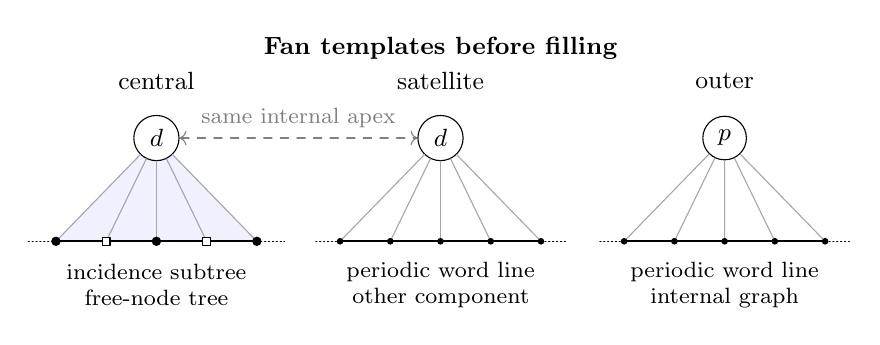
\begin{tikzpicture}[x=.88cm,y=.88cm,font=\small,
  every node/.style={align=center},line cap=round,line join=round,
  apex/.style={circle,draw,fill=white,inner sep=3pt},
  slot/.style={rectangle,draw,fill=white,inner sep=2pt}]
  \node[font=\small\bfseries] at (6,6.22)
    {Fan templates before filling};
  \node at (1.9,5.75) {central};
  \node at (6,5.75) {satellite};
  \node at (10.1,5.75) {outer};
  \fill[blue!6] (.45,3.43)--(1.9,4.92)--(3.35,3.43)--cycle;
  \node[apex] (dc) at (1.9,4.92) {$d$};
  \node[apex] (ds) at (6,4.92) {$d$};
  \node[apex] (po) at (10.1,4.92) {$p$};
  \draw[<->,dashed,gray] (dc)--node[above,font=\footnotesize]
    {same internal apex} (ds);
  \foreach \x in {.45,1.175,1.9,2.625,3.35} {
    \draw[gray!70] (dc)--(\x,3.43);
  }
  \draw[thick] (.45,3.43)--(3.35,3.43);
  \foreach \x in {.45,1.9,3.35} {\fill (\x,3.43) circle (1.7pt);}
  \foreach \x in {1.175,2.625} {
    \draw[fill=white] (\x-.055,3.375) rectangle (\x+.055,3.485);
  }
  \draw[densely dotted] (.05,3.43)--(.45,3.43);
  \draw[densely dotted] (3.35,3.43)--(3.75,3.43);
  \foreach \offset/\tip in {4.55/ds,8.65/po} {
    \draw[thick] (\offset,3.43)--(\offset+2.9,3.43);
    \draw[densely dotted] (\offset-.35,3.43)--(\offset,3.43);
    \draw[densely dotted] (\offset+2.9,3.43)--(\offset+3.25,3.43);
    \foreach \step in {0,.725,1.45,2.175,2.9} {
      \draw[gray!70] (\tip)--(\offset+\step,3.43);
      \fill (\offset+\step,3.43) circle (1.2pt);
    }
  }
  \node[font=\footnotesize,text width=3cm] at (1.9,2.8)
    {incidence subtree\\free-node tree};
  \node[font=\footnotesize,text width=3cm] at (6,2.8)
    {periodic word line\\other component};
  \node[font=\footnotesize,text width=3cm] at (10.1,2.8)
    {periodic word line\\internal graph};
\end{tikzpicture}
\caption{The three fan types before filling. The two $d$-symbols are
separate templates for one physical internal apex. Central fans cone
incidence subtrees in free-node Cayley trees; dots are ordinary sites and
small squares are horizontal midpoints. Satellite fans cone indexed word
lines mapping into other central components. Distinct satellite arms at
$d$ target distinct components in the developed model. An outer fan has
its own apex $p$ and an indexed word line mapping into the internal graph.
The word-line maps may repeat physical vertices and edges; their tags
retain the occurrences. The drawings are schematic and impose no planar
geometry.}
\label{fig:fan-templates}
\end{figure}


Let $K_J$ be the total kernel of the standalone induced filling of $J$,
and write
\[
 \overline{\mathcal X}=K_J\backslash\mathcal X,
 \qquad \mathcal A=\overline{\mathcal X}^{(1)}.
\]

\begin{lemma}[The filled model]\label{fan:filled-model}
For sufficiently deep choices, $\overline{\mathcal X}$ is simply
connected and $\mathcal A$ is uniformly hyperbolic.  The action of
$\bar J=J/K_J$ is cocompact, has free regular vertices and oriented
edges, and has exact finite apex stabilizers $\bar P=P/N_P$.
For each fixed filling, $\mathcal A$ is locally finite and proper, and
$\bar J$ is hyperbolic.

The central link $L_N(d)$ at an internal apex is the disjoint union of
its incidence subtrees modulo $N_P$.  Its components are exactly the
Stallings covers determined by $M\cap N_P$.  Satellite arms become
indexed path cycles of period $n=|\bar c|$; an outer apex has its one
indexed boundary cycle.  Period is measured in generator steps, with
bounded fractional offsets within the chosen word path.
\end{lemma}

\begin{proof}
The kernel $K_J$ is generated by conjugates of peripheral kernel
elements, each of which fixes an apex of $\mathcal X$.  A loop in the
quotient lifts edge by edge to a path upstairs with endpoint discrepancy
in $K_J$.  Express that discrepancy as a product of vertex-fixing
elements.  For each factor insert a path to its fixed apex followed by
the translated reverse path.  Its projection is a backtrack through
that apex.  The resulting closed path upstairs contracts because
$\mathcal X$ is simply connected.  This proves simple connectivity
of the quotient.

Exact peripheral reduction gives
$K_J\cap P=N_P$.  Two tags at a specified apex are consequently
identified precisely by $N_P$, proving the link assertion.  In
particular there is one apex for each marked coset, even when several
arms have that source.  Regular frame labels and oriented edge labels
become free $\bar J$-labels.  The arm stabilizer acts on its abstract
indexed line by its specified generator, so its quotient has exactly
$|\bar c|$ periods.

Formula~\eqref{fan:frame-formula} maps every edge to a bounded path in
the coned Cayley graph of the induced peripheral structure.  Conversely,
connectivity of $\mathcal X$ supplies fixed paths implementing its
finite relative generators, changing regular site types, and reaching
representatives of every apex orbit.  These paths descend, with bounds
independent of the filling.  Thus $\mathcal A$ and that coned Cayley
graph are uniformly quasi-isometric.  The relative filling bounds
from Section~\ref{sec:transfer-relative} give uniform hyperbolicity.  There
are finitely many edge orbits, free regular stabilizers, and finite
apex stabilizers, so a fixed quotient graph is locally finite and the
action is proper and cocompact.  It follows that $\bar J$ is hyperbolic;
its ordinary Cayley-metric comparison constants need not be uniform
as the filling varies.
\end{proof}

\subsection{Angles, tags, and exact covers}

For germs $e,e'$ at an apex $s$, define $\angle_s(e,e')$ to be the
shortest path length between their other endpoints in
$\mathcal A\setminus\{s\}$, with value $\infty$ if no such path exists.
Parallel tagged germs are distinguished even when this angle is zero.

\begin{lemma}[The finite angle dictionary]\label{fan:angle-dictionary}
All of the following conditions can be imposed for any finite list of
bounds before choosing the filling.
\begin{enumerate}[label=\textup{(\roman*)}]
\item There are no self-spokes.  Two distinct central spokes from a
fixed apex do not end at the same physical horizontal midpoint, and
likewise do not end at the same ordinary site.
\item For each $R$, after the first germ is normalized to a fixed
representative, every second germ at angle at most $R$ is obtained by a
translator from a fixed finite list in the original peripheral group.
The list includes the two germ types and does not depend on the filling.
Consequently angular balls have uniformly bounded cardinality.
\item On one indexed arm, source germs at bounded angle have sites
whose cyclic period coordinates differ by a uniformly bounded amount.
\item Every bounded closed walk in which each apex is visited at most
once cyclically has a closed labeled lift to the original fan graph,
with its given edge types and projected incidences.
\item All arm orders used here can be chosen even and arbitrarily
large.
\end{enumerate}
\end{lemma}

\begin{proof}
The first assertion holds upstairs.  Satellite targets belong to
components different from their source component.  Within the central
bipartite tree, at most one incidence joins a specified pair of nodes,
and its incidence subtree is embedded in the free tree.  A violation
after filling would give an equality of endpoint frames, or membership
of a fixed offset in a specified peripheral coset.  There are finitely
many edge types, so the finite-element and coset-avoidance tests from
Section~\ref{sec:transfer-relative} exclude these violations.

For the second assertion, expand an avoiding path in $\mathcal A$
using~\eqref{fan:frame-formula}.  Add its finitely many offsets to the
ordinary generating letters before setting the depth.  Each expanded
edge uses ordinary offsets and, when necessary, the cone legs at its
endpoints.  Neither endpoint is $s$.  Even when a germ's other endpoint
is a different apex, its connection to the designated ordinary germ
coordinate uses only fixed offsets and that other apex's cone leg.
Thus the expanded bypass still avoids the marked coset apex $s$.
Closing it across the two germs gives an isolated peripheral component.
The isolated-component bound for the uniformly linear relative
presentations, as used in Section~\ref{sec:transfer-relative}, places its
translator in a fixed finite set of actual peripheral elements
\cite{Osin2006,Osin2007}.  Tags and their free edge frames bound the
number of germs represented by that list.

For two sites on the same arm, normalize both word phases and write
the relative rotation as a power of its generator $c$.  The finite list
just obtained must lie in the image of $\langle c\rangle$.
Finite-list membership avoidance inside the ambient hyperbolic VCS
periodic peripheral ensures that such membership already holds before
filling.  Since $N_P$ lies inside the chosen base finite-index subgroup,
that test remains valid for the final kernel.  Each actual list element
then has a fixed exponent in $\langle c\rangle$, proving the period
bound.  For an outer cyclic peripheral this is immediate.  Word phases
only change the bound by a fixed amount.

For the fourth assertion, the rest of the closed walk is an avoiding
path at each of its apex visits.  Replace the successive normalized
peripheral transporters by elements of the finite lists in the second
assertion.  At regular vertices the transitions are fixed offsets.
After normalizing an initial oriented edge, the closing equation is
one of finitely many actual word equations.  Injection on that finite
set makes it hold upstairs.  This constructs one closed labeled lift;
it does not assert compatible lifts of arbitrarily many independent
translates.  That stronger assertion will not be needed.

Finally use the divisible order choices and exact order conclusions
of Proposition~\ref{kernel:orders}.  Only finitely many bounds and element
lists have been imposed, so all the choices are simultaneous.
\end{proof}

\begin{lemma}[Exact graph-cover data]\label{fan:cover-data}
Let $H_P$ be the intersection of a periodic peripheral's normal base
choice $H$ with $P_d$, and let $L_H(d)$ be its central link modulo
$H_P$.  Its finitely many components can be required to have
arbitrarily large girth.  Over each connected component $B$ there is a
nonempty finite collection of connected cyclic $\ell$-covers
$B_j\to B$, where $\ell>1$, and a finite field $\mathbb k$ with
$\operatorname{char}\mathbb k\nmid\ell$.  The corresponding component
of $L_N(d)$ is exactly the cover associated to the intersection of
\begin{enumerate}[label=\textup{(\roman*)}]
\item the kernels of all these cyclic covering maps; and
\item inside each covering kernel, the kernels of all additive first
cohomology classes in the nontrivial deck part of
$H^1(B_j;\mathbb k)$.
\end{enumerate}
The assertion holds also for the cyclic root incidences, whose
nontrivial deck cohomology part is zero.
\end{lemma}

\begin{proof}
Apply Corollary~\ref{kernel:graph-cover} to the actual free-row incidence
$M$.  In the unclaimed-root expansion, an elliptic $M_x^d$ is precisely
the corresponding free-edge-level incidence group, so the same
restriction theorem applies.  Its exact restriction statement is what
gives equality with the stated intersection, rather than merely a
cover factoring through it.  Conjugations and coset versions are
included in the kernel choices.  For root cyclic incidences use
Remark~\ref{kernel:cyclic-peripheral}: the character is surjective
modulo $\ell$ on the required intersection, and a cyclic group's first
cohomology has no nontrivial deck part.  Finally there are finitely many
original Stallings core types.  Residual finiteness of the ambient
periodic peripheral separates all their nonzero circuits of any fixed
length, giving the girth requirement before the character choices.
\end{proof}

\subsection{Large-angle comparisons}

We record the geometry used at each later wall gluing.  All constants
in this subsection depend on uniform hyperbolicity and the displayed
quasigeodesic constants, not on the final peripheral orders.

\begin{lemma}[Forced passage and marker comparison]
\label{fan:marker}\label{fan:marker-comparison}
In a uniformly hyperbolic graph the following hold.
\begin{enumerate}[label=\textup{(\roman*)}]
\item Geodesic legs from $s$ with sufficiently large angle concatenate
to a geodesic, and every geodesic between their other endpoints passes
through $s$.
\item Two uniform quasigeodesics from $s$ to the same finite or ideal
endpoint, neither revisiting $s$, have departure germs at bounded
angle.  If a geodesic has a sufficiently large interior angle at $s$,
a uniform comparison quasigeodesic cannot avoid $s$.  Nor can all its
germs at $s$ have a previously prescribed bounded angular diameter.
\item Suppose uniform quasi-isometrically embedded tree pieces are
joined by switches whose spokes have uniformly bounded lengths.
A switch maps to a marker in the graph.  For every reduced incidence
path, assume each connector through a piece has distinct endpoint
markers and avoids them except at its endpoints.  Impose the same
conditions on partial connectors at marked-node endpoints.  Assume
also that each piece attaches at most once at a given marker, and
that all distinct spoke germs at each switch have pairwise angle
larger than a sufficiently large fixed threshold.
Then the joined components are uniformly quasi-isometrically
embedded trees.  Their node projections are injective provided the
piece node projections are injective and the stated endpoint
conditions hold.  Every interior switch on a reduced path is a
large-angle turn on a geodesic between its projected endpoints.
The same conclusion holds towards an ideal endpoint of a ray when
the ambient graph is proper.
\end{enumerate}
The quasi-isometry constants in the third assertion can be fixed after
one minimum angle threshold is met.  Increasing the angle threshold
later increases the forced comparison angle without changing those
constants.
\end{lemma}

\begin{proof}
For the first two assertions use thin triangles and quasigeodesic
stability.  If a comparison path avoids $s$, choose points a sufficiently
large fixed distance out on the two relevant legs, using the endpoints
when a leg is shorter.  Thinness gives bounded bridges to the other
leg or to the comparison path.  Take the bridge points far enough
from $s$ that the bridges avoid it.  The portion of the comparison path
between the bridges has bounded length; for a quasigeodesic this follows
from its quasigeodesic inequality.  These paths give a bounded bypass
between the initial germs.  Thus a sufficiently large angle precludes
an avoiding geodesic and forces passage through $s$.  Its two subpaths
then have the lengths of the original legs, proving the concatenation
claim.  The same construction compares two departures to a common
endpoint.  For ideal endpoints first work on long finite initial
segments and use stability; properness supplies limiting geodesics
when required.  Finally, if the comparison path visits $s$, compare its
first and last visits towards the two endpoints.  A large geodesic
angle forces large angular diameter between these two comparison
germs.

For the gluing assertion, every piece connector is a uniform
quasigeodesic: adding bounded end spokes to a uniformly embedded
piece path changes only its additive constants.  The endpoint
avoidance hypotheses allow its departure and arrival germs to be
compared with those of a geodesic replacement.  The angle error is
bounded by the second assertion.  Hence consecutive replacement
geodesics still make an arbitrarily prescribed large angle at their
common switch if the spoke threshold is chosen sufficiently large.

Apply the first assertion inductively along a reduced incidence path.
The concatenation of its geodesic replacements is a geodesic, and
every interior switch remains a large-angle vertex on it.  A circuit
not contained in a piece would therefore give a positive-length
geodesic returning to its start; a circuit within a piece is impossible
because the piece is a tree.  Reusing one attachment does not create an
exception, since the incidence path was reduced and each piece has at
most one attachment at that marker.  The same argument rules out
repetition of node projections across switches; within pieces use the
assumed injectivity.

There are uniform constants $a,b$ such that the intrinsic length of
each connector is at most $a$ times the length of its geodesic
replacement plus $b$.  Distinct marker vertices have distance at least
one.  Summing over connectors therefore absorbs their additive errors
into a uniform multiplicative bound; the two end errors remain
uniformly bounded.  This proves quasi-isometric embedding.  Bounded
initial or terminal portions of spokes do not affect it.  Taking limits
proves the ray statement.  None of these estimates improves or worsens
when the angles are increased above the fixed minimum.
\end{proof}

\subsection{Sparse cuts from exact homological covers}

A \emph{central panel} $b$ at $d$ is a function
$\zeta_b:V(L_N(d))\to\{0,1\}$, defined on all ordinary link vertices.
Its \emph{cuts} are link edges with unequal endpoint labels.  The
corresponding cut germs are the central spokes to their midpoints.

\begin{proposition}[Central panel tests]
\label{fan:central-panels}\label{fan:sparse-panels}
Fix $K$, a bound $q$ on the number of target link vertices, and a bound
$r$ on the number of prescribed directions at an internal apex.
There is a bound $B$, depending only on these bounds and the fixed
original data, with the following property after suitable kernel
choices.  For every such target list and direction list there is a
partition of the targets into classes, each in one component of $L_N$
and of intrinsic diameter at most $B$, such that every binary
assignment to these classes extends to a central panel.  Its cut germs
are pairwise at angle greater than $K$, and all are at angle greater
than $K$ from the prescribed directions.  The same partition works
for all binary assignments.

There are also fillers: for every occurrence of a link edge there is
a panel cutting that occurrence whose cuts all lie over its one base
edge in $L_H$.  Its cut germs can be required pairwise farther than
$K$.
\end{proposition}

\begin{proof}
We first arrange that different lifts of any one edge of $L_H$ are
angularly farther than $K$.  Normalize their first tagged spoke by a
peripheral translator.  A short angle would, by
Lemma~\ref{fan:angle-dictionary}, give a translator from a fixed finite
actual list.  Since the lifts have the same image modulo $H_P$, its
image belongs to $H_P/N_P$.  Normality of $H$, and $N_P\le H_P$, put
the actual list element in $H_P$.  Choose $H$ to exclude all nonidentity
members of this list.  The remaining identity cannot identify two
different tagged spokes, whose stabilizers are trivial.

Select support base edges successively.  At each stage forbid all
base edges having a lift angularly near a prescribed direction or
near any lift of a support edge already chosen.  The number forbidden
by a direction is uniformly bounded.  The number forbidden by one
support edge is also uniformly bounded: the deck group $H_P/N_P$ is
transitive on all its tagged lifts, so normalize one lift and apply
the finite angle dictionary.  We will make at most $\binom q2$
selections.  There is consequently a uniform bound $B$ for the total
number of forbidden edges at every stage.  Enlarge $B$ if necessary
and require every $L_H$-component to have girth greater than $B$.
The forbidden-edge subgraph, including its isolated vertices, is then
a forest.

Here is the separation assertion underlying the construction.  Let
$u,v$ lie in one $L_N$-component, and let $F$ be its forbidden base
forest.  If $d_{L_N}(u,v)>B$, an allowed support edge supplies a
potential distinguishing them.  To prove this, choose a joining path
and project its chain to each cyclic cover $B_j$ from
Lemma~\ref{fan:cover-data}; call the chain $c_j$.  Put
\[
 A_j=\frac1\ell\sum_{g\in\operatorname{Deck}(B_j/B)}g
\]
for deck averaging on chains and cochains.  For each allowed base edge,
differences of the cochains on two of its individual oriented lifts
have coefficients $1,-1$ and lie in $\ker A_j$.  Their cohomology
classes belong to the nontrivial deck part.  Their pullbacks to $L_N$
are exact by the defining kernel property, hence are differentials
of $\mathbb k$-valued potentials.

Suppose none of these potentials distinguishes $u,v$.  Evaluation on
the projected path says that all coefficients of $c_j$ over any allowed
edge are equal.  Therefore
\begin{equation}\label{fan:forest-chain}
 (1-A_j)c_j\quad\hbox{is supported on the inverse image of }F,
 \qquad
 \partial(1-A_j)c_j=(1-A_j)([v_j]-[u_j]).
\end{equation}
Each lift of a base tree of $F$ is a tree, and there are $\ell$ such
lifts.  The augmentation of a boundary on each lifted tree is zero.
If the base projections of $u,v$ belonged to different base trees,
the right side of~\eqref{fan:forest-chain} would have nonzero
augmentation on at least one lift of either tree: its endpoint mass
is the difference between one point and its deck average, and
$\ell>1$ with $\ell$ invertible in $\mathbb k$.  The base endpoints
must therefore belong to one forest tree.  Their deck-average masses
on each lift cancel, so the same augmentation test forces $u_j,v_j$
to lie in the same lift of that tree.

Let $f$ be the unique base forest path between the two base endpoints.
It lifts to a path $f_j$ from $u_j$ to $v_j$ in every $B_j$.  The chains
$(1-A_j)c_j$ and $(1-A_j)f_j$ have the same boundary and are both
supported on a forest.  A forest has no nonzero one-cycles, so they
are equal.  Thus $c_j-f_j$ is invariant under deck averaging.  The
comparison loop belongs to every cyclic-cover kernel and evaluates
to zero on every nontrivial deck cohomology class.  Exactness in
Lemma~\ref{fan:cover-data} puts it in the final covering kernel.
Consequently $f$ lifts between the original $u,v$ in $L_N$, giving
$d_{L_N}(u,v)\le |F|\le B$, a contradiction.  This proves the
separation assertion.

Now process all same-component target pairs at distance greater than
$B$.  Select an allowed support edge and a distinguishing potential
for each pair still requiring distinction.  Extend each potential
constantly on the other components.  Two targets are put in the same
class precisely when they belong to the same component and have the
same tuple of potential values.  The separation assertion gives the
claimed diameter bound.  Any prescribed binary values on the target
classes extend to a binary function of this tuple and the component
identifier, assigning arbitrary values on the remaining tuples.
Its gradient is supported only over the selected support edges.
The forbidden-edge rule separates different support edges, while
the first paragraph separates different lifts of one support edge.
This proves both cut separation and avoidance of the direction list.

For a filler, choose a cyclic cover over the component in question
and take the difference cochain between the lift containing the
specified occurrence and a different lift of its base edge.  Its
pullback is exact and its value on the specified edge is nonzero.
A binary separation of the two endpoint potential values therefore
cuts that occurrence, with all cuts over that one base edge.  This
argument only requires the nontrivial covering degree.  In particular,
when the nontrivial cohomology itself is zero, the difference cochain
is already exact but still has a nonconstant potential.  The proof
works unchanged in characteristic two when $\ell$ is odd.
\end{proof}

\subsection{Central trees and their cochains}

For the actual finite links, take finite systems realizing all required
panel tests and then all peripheral translates.  Decorate panels by
free regular $\bar P_d$-multiplicities so that the data, rather than only
their isomorphism classes, translate equivariantly.  There are finitely
many requested orbits.  We next equalize their numbers of cuts.

For each central spoke orbit type, a peripheral orbit of fillers adds
a positive constant number of cuts at every spoke of that type and
none of the other types.  Multiply the requested systems by a common
multiple of these positive numbers.  Choose a common larger integer
$l$ divisible by all of them, and top up each type using its fillers.
Thus exactly $l$ cutting panels occur at every central spoke to a
midpoint.  The same $l$ can be used for all finitely many types.
Decorate every physical horizontal midpoint by $l$ slots, including
midpoints untouched by a particular panel system.  At each apex
incidence match the slots bijectively with its cutting panels.
Choose this matching equivariantly: the horizontal edge frames are
free, and Lemma~\ref{fan:angle-dictionary} gives only one central
occurrence from this apex at the specified midpoint.  Join a panel
to its assigned slots by edges projecting to its cut spokes.

\begin{lemma}[Central trees]\label{fan:central-trees}
Every component $W_0$ of the panel--slot graph is a uniformly
quasi-isometrically embedded tree in $\mathcal A$, injective on node
projections.  Its constants require only a minimum cut-angle threshold
and remain valid when subsequent panel systems use larger thresholds.
There are finitely many decorated node and edge orbits.  Distinct
systems may be retained separately as a finite labeled pool.
\end{lemma}

\begin{proof}
Apply Lemma~\ref{fan:marker} with slots as point pieces and panels as
switches.  Along a reduced path the two panel markers adjacent to one
slot are distinct: from a fixed apex, that slot is matched to only one
cutting panel.  The two-spoke connector through the slot avoids its
endpoint apices, and each point piece attaches at most once over any
apex.  At a panel all cut germs have the stipulated large angle.
The marker lemma proves both the tree assertion and injectivity on
nodes.  Finiteness of the orbit data follows from finite links, finite
peripheral reductions, and the finite multiplicities just chosen.
\end{proof}

A horizontal edge is \emph{marked by $W_0$} when its midpoint has a
slot in $W_0$, necessarily unique.  At an incident central link edge,
that slot belongs to $W_0$ precisely together with its matched cutting
panel.  There is at most one panel of $W_0$ above any given apex.

\begin{lemma}[The central cochain]\label{fan:central-cochain}
Each $W_0$ carries an equivariant mod-two cochain $\tau_0^{W_0}$ on the
central complex, closed on every central face.  It has value one on
the positive initial half of each marked horizontal edge, zero on all
other horizontal halves, and value $\zeta_b(t)$ on an ordinary radial
edge $d\!-\!t$ when its panel $b$ belongs to $W_0$, or zero when there
is no such panel.  Every edge with nonzero value has a panel or slot
anchor of $W_0$ at one of its endpoints.
\end{lemma}

\begin{proof}
The assertions specify the ordinary radial and horizontal values.
For an edge with positive orientation $u\!-\!m\!-\!v$, let
$\epsilon$ indicate whether it is marked.  Put the midpoint radial
value equal to $\zeta_b(u)+\epsilon=\zeta_b(v)$, taking the ordinary
radial labels to be zero if $b$ is absent.  The equality follows from
the matching rule: the link edge is a cut exactly when its slot and
cutting panel lie in this tree.  Both fan triangles therefore have
zero boundary sum.  These are all central faces.  The formulas also
give the anchor assertion and are preserved by the decorated group
action.
\end{proof}

\begin{lemma}[Satellite arm exclusivity and bounded support]
\label{fan:arm-exclusivity}
If $W_0$ has a node anchored on a satellite arm of $d$, then it has no
node over $d$ and no anchor on a different satellite arm of the same
$d$.  All its anchor occurrences on that arm, and all nonzero
occurrences of $\tau_0^{W_0}$ on its boundary cycle, lie in a period
interval of uniformly bounded diameter.  These bounds are independent
of the arm order and of later increases in cut separation.

If $\tau_0^{W_0}$ has odd total on the arm cycle, its stabilizer inside
$\bar P_d$ is trivial.
\end{lemma}

\begin{proof}
An anchor on the arm is joined to $d$ by its tagged source spoke.
If $W_0$ contained $d$, its intrinsic path to that anchor would have
uniformly bounded length by Lemma~\ref{fan:central-trees}.  Close it
by this spoke.  Likewise, anchors on two arms can be joined through
$d$ by two spokes, so their intrinsic $W_0$ path has uniformly bounded
length.  In the latter case $d$ has already been excluded.  These
closed walks are apex-simple: $W_0$ is injective on node projections
and its edges are central spokes, while the added source apex occurs
only at the cyclic joining point.  Lemma~\ref{fan:angle-dictionary}
therefore supplies a closed labeled lift upstairs.

The lift of the $W_0$ segment is a central path.  In the first case it
would join $d$ to a target component of its satellite arm, contrary to
Lemma~\ref{fan:components}.  In the second case it would join the
targets of two distinct arms in one central component.  The arms
remain distinct upstairs: at a fixed source, their incidence tags
are cosets $P_d/\langle c\rangle$, and the quotient construction gives
the corresponding cosets in $\bar P_d$.  If two lifted incidences
were the same, their projected incidences would be the same.  Thus one
closed polygon lift suffices for this contradiction; no simultaneous
lifting of independently chosen translates is being assumed.

The path in $W_0$ between two anchors on the one remaining arm has
bounded length, using the two-spoke shortcut through $d$, and avoids
$d$.  Apply the period part of Lemma~\ref{fan:angle-dictionary} to
obtain the bounded interval.  A nonzero central cochain occurrence
has an anchor at an endpoint, and the word paths have fixed lengths,
so a fixed enlargement of this interval contains its support.

An odd total makes the support nonempty.  Any element of $\bar P_d$
stabilizing $W_0$ must preserve its unique encountered arm.  That arm's
stabilizer acts faithfully by rotations of its tagged period cycle.
For order sufficiently large compared with the support diameter, no
nonidentity subgroup of this rotation group preserves a nonempty
subset contained in such a short interval.  This proves the last
assertion.  All bounds used the minimum quasi-isometry constants and
fixed word lengths, so increasing the cut threshold does not change
them.
\end{proof}

\subsection{Odd seeds on satellite arms}

\begin{proposition}[Odd inner seeds]\label{fan:odd-seeds}
A finite pool of central panel systems, chosen at successive fixed
angle scales, can be required to contain, on every satellite arm, a
central tree $W_0$ for which $\tau_0^{W_0}$ has odd total on the arm's
boundary cycle.  The choices and all support bounds are independent
of the sufficiently large individual cycle orders.
\end{proposition}

\begin{proof}
Fix an arm cycle $\beta$ with source $d$ and period $n$.
At each internal apex $s$ visited by its central boundary path, list
all radial half-incidences, with multiplicity.  Their other endpoints
are ordinary by construction.  The list size is uniformly bounded:
all source spokes from $d$ to the repeated occurrence of $s$ have the
same other endpoint, hence angle zero at $d$; the finite angle
and period dictionaries bound both their number and their period
spread.  At $s$ the listed directions are mutually close in angle by
paths through $d$.

Use Proposition~\ref{fan:central-panels} with cuts sufficiently far
from these directions and with every binary assignment on its bounded
diameter target classes.  For the tree through such a testing panel
at $s$, no other anchor $w\ne s$ lies on $\beta$.  Indeed the arm
exclusivity lemma excludes $d$ from this tree.  Its path from $s$ to
$w$ can be compared with the path $s\!-\!d\!-\!w$ of length at most
two.  The first germ of the latter is close to every listed direction
at $s$, by the adjacent ordinary site on $\beta$.  Departure comparison
in Lemma~\ref{fan:marker} contradicts the first cut's chosen distance
from those directions.  The cochain's total on $\beta$ is therefore
exactly the sum of the tested labels at $s$.

If any test has odd total, it supplies the seed.  Otherwise every
target class occurs an even number of times.  Pair the radial
half-incidences within each class and replace each pair, as a mod-two
chain, by a horizontal link path between its two ordinary sites.
The paths have a uniform length bound $B_1$.  Fan triangles show that
each replacement preserves evaluation by every central cochain.
Perform this at all visited apices.  The result is a finite purely
horizontal cycle chain $z$; connectivity is not required.

We justify that $z$ is nonzero by retaining its winding around the
period circle $C_n=\mathbb R/n\mathbb Z$.  Initially each occurrence
on $\beta$ has its indexed period coordinate, with the fixed
fractional coordinates inside a word.  Every vertex occurrence added
by a replacement has a horizontal tail of length at most $B_1$ to
one of the original ordinary sites.  Two occurrences representing the
same physical vertex thus have original sites joined by a bounded
path avoiding $d$.  Their source spokes have bounded angle at $d$,
so their period coordinates differ by a fixed bounded amount.
The same applies to the two occurrences of $s$ involved in each
paired replacement.  Consequently each replacement polygon, and
all ambiguity in assigning coordinates to one physical vertex,
occupies a period interval of bounded diameter.

For completeness, let $T$ bound horizontal replacement lengths in
our subdivided metric, and let $D(R)$ be the period-coordinate bound
for original occurrences joined by a path of length at most $R$
avoiding $d$.  Enlarge it monotonically and put
\[
 M=\max\{1,D(T),D(2T+1)\},\qquad n>8M.
\]
For every physical vertex in the finite graph used by $\beta$ and
the replacements, choose one original occurrence reachable by a
horizontal tail of length at most $T$, and assign its period
coordinate to the vertex.  Original vertices, including apices,
allow the zero-length tail.  Map each physical edge by the unique
short arc between its assigned endpoint coordinates.  The assigned
coordinate at an original occurrence differs from its parameter
coordinate by at most $M$.  Along the indexed original cycle choose
these errors in $[-M,M]$.  Each elementary parameter increment is
at most one, so its adjusted increment has absolute value at most
$1+2M<n/2$ and is exactly the chosen short-arc increment.  The errors
telescope around the cycle, leaving total increment $n$ and degree
one.  For a replacement polygon centered at an occurrence of $s$,
the witness original occurrence of any of its vertices is joined
to that $s$ by an avoiding path of length at most $2T+1$.
All assigned coordinates therefore lie in one interval of length
at most $2M<n/2$.  Its edge images stay in that interval, so the
polygon has degree zero.  The image of
$z$ thus has degree one modulo two.  In particular some physical
horizontal edge occurs in $z$ with coefficient one.  At its midpoint
the cycle equation makes the two half-edge coefficients equal.

Choose a second central panel system with cut angles larger than a
threshold fixed after $B_1$, and take the central tree through a slot
of that edge.  It has no node above $d$.  Otherwise close its bounded
path to the slot by the slot's bounded horizontal tail to an original
arm site and the source spoke to $d$.  The added tail has no apices,
so the resulting bounded walk is apex-simple and lifts by
Lemma~\ref{fan:angle-dictionary}.  Its lifted central path would join
$d$ to the target component, the contradiction used in
Lemma~\ref{fan:arm-exclusivity}.

Nor can this tree contain two distinct horizontal anchors of $z$.
Each anchor has a bounded horizontal tail to $\beta$, and hence a
bounded path to $d$.  Between two distinct slot nodes the tree path
has an interior panel marker, different from $d$.  Its angle is larger
than the fixed comparison threshold.  The path between the two
anchors formed from their horizontal tails and the two source spokes
through $d$ has uniformly bounded length and avoids every such marker.
It is a uniform comparison quasigeodesic, with constants depending
only on that length bound.  Lemma~\ref{fan:marker} gives a
contradiction.  Thus the chosen tree has exactly one horizontal anchor
on the support of $z$.  Its cochain evaluates to one there, and hence
to one on $z$ and on the original $\beta$.

There are only finitely many actual links and bounded-size requests
for a fixed filling.  Include all first-stage tests, their translates,
and the second-stage filler systems.  The constants determining these
requests were fixed independently of $n$, so this is a finite pool
working for every sufficiently deep filling and every arm type.
\end{proof}

\subsection{Order and uniformity of the choices}\label{fan:scale-order}

We make explicit the quantifier order used here and in the next
section.  First fix the original row types, their word paths, the
uniform relative hyperbolicity bounds, and a minimum bend threshold
in Lemma~\ref{fan:marker}.  This fixes the quasi-isometry constants of
the central trees and the arm-support bounds in
Lemma~\ref{fan:arm-exclusivity}.  Any larger cut separations preserve
these constants.

Next prescribe the finitely many target-list sizes and direction
avoidance thresholds that will be tested.  Proposition~\ref{fan:central-panels}
provides a bound for the number of forbidden base edges and for the
resulting class diameters, independently of $H$ and $N_P$.  For odd
seeds, choose the first testing threshold, compute its replacement
bound $B_1$, and only then choose the second cut threshold needed to
exclude the bounded comparison paths.  The two systems remain
separately tagged: the first-stage class bound is not recomputed
using the second threshold.  All angle dictionaries and
short-polygon lifting tests at these finitely many scales are now
fixed.  Subsequent applications may repeat this finite procedure,
provided each new threshold depends only on already fixed bounds.

Finally choose the normal base subgroups $H$ to meet all resulting
finite-list exclusions and girth bounds.  Apply the character and
cohomology kernel construction, preserving those tests because
$N_P\le H_P$.  Choose the cyclic orders even and larger than the
finitely many period and support bounds.  The graph-cover argument
uses the number of target pairs, not the number of characters or the
size of a final link, so enlarging a cover at this last stage does not
alter any previously fixed bound.  All these choices are compatible
with any initial finite-path filling requirements by
Proposition~\ref{kernel:construction}.

The outgoing data are therefore a finite pool of equivariant central
trees $W_0$, their central cocycles $\tau_0$, arbitrary prescribed panel
tests of the stated bounded type, and odd inner seeds with uniformly
bounded support and free arm stabilizers.  These are the data used to
attach the satellite and outer switches.

\section{Switches, cocycles, and boundary separation}\label{sec:10-boundary}

Our goal is to separate every pair of boundary points by a quasiconvex
subgroup, so that the boundary criterion gives a cocompact cubulation
of each filled row. We first extend the central trees and cocycles
across the satellite fans and then the outer fans. The second half
of the section proves that the resulting cocycles supply all the
required separators.

We continue with a terminal vertex row $J=Y_v$ and the filled fan complex of
Section~\ref{sec:09-fans}. Its edge graph is $\mathcal A$ and its acting group
is $\bar J$. In particular, $\mathcal A$ is uniformly hyperbolic, and, for each
individual filling, it is locally finite and the action is proper and
cocompact. Internal and outer apices are denoted by $d$ and $p$, respectively.
All the choices below are made simultaneously over the finitely many row
types. The initial filling depth, and the finite tests required by
Section~\ref{sec:transfer-relative}, may be prescribed in advance.

All chains and cochains in this section have coefficients in $\F_2$.
Occurrences of edges are retained with multiplicity until a pairing is made;
only then do we reduce modulo two. Thus a passage through an apex supplies two
radial half-incidences, even when it uses the same physical edge twice. A
\emph{pure internal} path avoids outer apices and uses true ordinary neighbors
at every internal apex and horizontal midpoint. The boundary word of every
satellite or outer fan has this property. Pair replacements will produce
chains, and these need not be connected.

We use the central trees $W_0$ and their cocycles $\tau_0$ from
Lemmas~\ref{fan:central-trees} and~\ref{fan:central-cochain}. An
\emph{anchor} is a projected panel or slot node of such a tree, and later also
a switch node. In particular, a central radial contribution has a panel
anchor at its apex, whereas a horizontal contribution has a slot anchor at
its midpoint. The angle dictionary of Lemma~\ref{fan:angle-dictionary} and
the marker comparison of Lemma~\ref{fan:marker} will always be used with
bounds fixed before the final filling kernels are chosen. We give the full
order of these choices at the end of the section.

\subsection{Nonmixed panels and the first switches}

At an internal apex $d$, central and satellite incidences can coexist.
Central labels prescribe values on the radial edges of incidence subtrees;
satellite labels must instead integrate cochains around the attached
cycles. We put these two kinds of labels on separate panel vertices.
Thus testing satellite labels at $d$ introduces no central labels there,
and a central panel acquires no satellite attachment at its own apex.
The later separation proofs will still check the contributions transmitted
through other apices.

\begin{definition}\label{boundary:total-panels}
A \emph{side} is a pair $(W_0,a)$ where the central tree $W_0$ has an
anchor occurrence on the boundary of an actual satellite arm $a$ at its
source $d$. The tree retains its system label and,
when copies are taken, its copy index. The side is \emph{odd} if
$\tau_0^{W_0}$ has total one on the indexed boundary cycle of $a$.
Consuming this side means assigning this particular incidence to one
satellite panel and choosing an anchor occurrence on $a$ for its attachment.

A \emph{central-only total panel} is a central panel $b$, with no additional
attachment at $d$. A \emph{satellite-only total panel} $T$ has no central
panel and consumes finitely many odd $W_0$-sides on the satellite arms at
$d$, an even number on each arm. For every consumed side, attach a spoke
from $T$ to its chosen anchor occurrence. The spoke projects to that tagged
satellite radial edge. Its germ at $d$ is required to be far from every
other spoke germ of $T$.

On each satellite arm, the binary labels of $T$ are a primitive of the sum
of the boundary cochains of the sides it consumes there. Such a primitive
exists because the number of odd sides is even. Its additive constant is
chosen independently on each arm. Central labels of $T$ are zero. Empty
satellite-only panels, including their independent constant labels, are
allowed.
\end{definition}

Figure~\ref{fig:fans-nonmixed-panels} shows these two kinds of abstract
panel over one physical apex. The fan spaces themselves were shown in
Figure~\ref{fig:fan-templates}.
\begin{figure}[tbp]
\centering
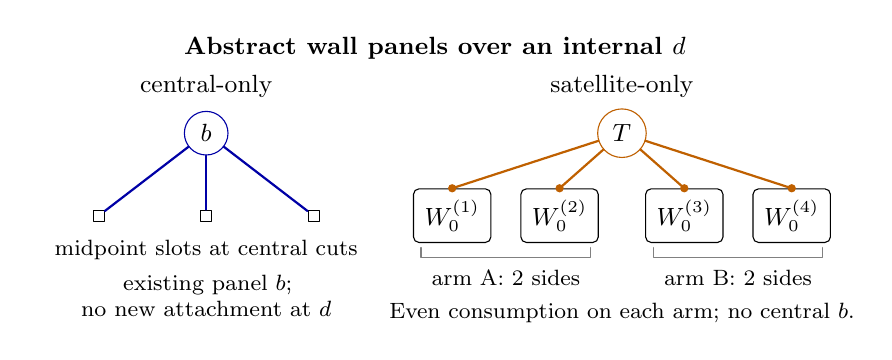
\begin{tikzpicture}[x=.88cm,y=.88cm,font=\small,
  every node/.style={align=center},line cap=round,line join=round,
  apex/.style={circle,draw,fill=white,inner sep=3pt},
  slot/.style={rectangle,draw,fill=white,inner sep=2pt}]
  \node[font=\small\bfseries] at (6,1.8)
    {Abstract wall panels over an internal $d$};
  \node at (2.7,1.24) {central-only};
  \node at (8.7,1.24) {satellite-only};
  \node[apex,draw=blue!65!black] (bc) at (2.7,.57) {$b$};
  \node[apex,draw=orange!75!black] (ts) at (8.7,.57) {$T$};
  \foreach \x/\name in {1.15/c1,2.7/c2,4.25/c3} {
    \node[slot] (\name) at (\x,-.62) {};
    \draw[thick,blue!65!black] (bc)--(\name);
  }
  \node[font=\footnotesize] at (2.7,-1.12) {midpoint slots at central cuts};
  \node[font=\footnotesize,text width=4.3cm] at (2.7,-1.78)
    {existing panel $b$;\\no new attachment at $d$};
  \foreach \x/\i in {6.25/1,7.8/2,9.6/3,11.15/4} {
    \node[draw,rounded corners=2pt,inner sep=4pt] (w\i)
      at (\x,-.62) {$W_0^{(\i)}$};
    \draw[thick,orange!75!black] (ts)--(w\i.north);
    \fill[orange!75!black] (w\i.north) circle (1.5pt);
  }
  \draw[gray] (5.8,-1.08)--(5.8,-1.22)--(8.25,-1.22)--(8.25,-1.08);
  \draw[gray] (9.15,-1.08)--(9.15,-1.22)--(11.6,-1.22)--(11.6,-1.08);
  \node[font=\footnotesize] at (7.025,-1.52) {arm A: $2$ sides};
  \node[font=\footnotesize] at (10.375,-1.52) {arm B: $2$ sides};
  \node[font=\footnotesize] at (8.7,-2.02)
    {Even consumption on each arm; no central $b$.};
\end{tikzpicture}
\caption{Nonmixed panels in the filled complex. The central-only panel
$b$ and satellite-only panel $T$ are abstract wall vertices projecting to
one internal apex $d$. The former joins midpoint slots at its central
cuts. The latter joins chosen anchor occurrences (colored dots) in odd
sides $(W_0,a)$, consuming an even number on each arm; two per arm are
shown only as an example. Across labeled copies, every odd side is
consumed exactly once. A $W_0$-copy may still have sides at other source
apices. Spoke angles are large in the graph metric at the physical image
$d$, irrespective of the drawn Euclidean angles. No additional avoidance
of central cuts is required. A satellite-only panel contains no central
$b$, and its central labels are zero.}
\label{fig:fans-nonmixed-panels}
\end{figure}


\begin{lemma}[Satellite profile tests]\label{boundary:satellite-profiles}
Fix bounds on the number of target ordinary satellite sites and forbidden
germ directions at $d$, and fix an angular avoidance threshold. A finite
pool containing the odd seeds of Proposition~\ref{fan:odd-seeds} supplies
satellite-only panels whose labels realize every binary assignment to a
partition of the target list into classes. Each class lies on one arm and
has bounded cyclic period-coordinate diameter. Their spoke germs avoid the
forbidden directions and one another by the prescribed threshold. The
class-diameter bound and the required filling tests depend only on these
fixed requests and the original finite data.
\end{lemma}

\begin{proof}
On each arm, order the listed sites cyclically. Join consecutive listed
sites into one cluster when the intervening gap is smaller than a fixed
threshold $D$. There are at most as many clusters as targets, and the
diameter of each cluster is at most the number of targets times $D$. A
prescribed binary assignment changes value across an even number of the
cyclically ordered gaps. For each such change, place a translate of an odd
seed with its entire support cluster inside that gap. Its contribution
changes the primitive by one between the neighboring target clusters.

The seed's support has uniformly bounded width. Its chosen anchor rotates
freely, and the angle dictionary bounds the number of rotations whose spoke
lies angularly close to a forbidden direction or a previously placed
spoke. There are only boundedly many directions and earlier placements.
Choose $D$ larger than the support width, the required end margins, and the
number of forbidden positions. Every required placement is then possible.
The additive constant on the arm realizes the value on the first cluster.
If the assignment is constant, no seed is needed. All rotations are by
integral period steps; the fixed elementary word lengths only enlarge the
bounds by fixed factors. These choices involve satellite spokes and the
given forbidden directions; they impose no avoidance condition against
central cuts at $d$.
\end{proof}

\begin{lemma}[Equivariant consumption]\label{boundary:consumption}
After taking finitely many labeled copies of a finite pool of central
systems, every odd side can be consumed exactly once. This can be done
equivariantly, with finitely many decorated panel and edge orbits, while
including all the tests of Lemma~\ref{boundary:satellite-profiles} and any
fixed lower bound on switch angles.
\end{lemma}

\begin{proof}
For each of the finitely many apex types, include the full free
$\bar P_d$-orbits of the stipulated decorated profiles. For the actual
finite links, all requests involving lists of the bounded sizes form a
finite set, so this requires only finitely many profiles. Take $m$ copies of
the entire initial central systems, with trivial action on copy indices.

Consider an arm with even period $n$ and rotation generator $c$. The
requested profiles use any odd side and its translate by $c^{n/2}$ equally
often, because they form full $\bar P_d$-orbits. These two sides are distinct:
the support cluster is nonempty and short compared with $n$. Double the
requested multiplicities and choose $m$ even and larger than all the
resulting consumption counts. Each side then has an even number of unused
copies, equal to the number for its antipode.

Consume the unused copies by antipodal pair panels. The pair's germs have
arbitrarily large angle once the period-coordinate avoidance test is
imposed. An unordered pair may have an order-two stabilizer, but a free
orbit of \emph{decorated} pair panels uses two copies of each side in such a
pair. The even residual multiplicities therefore permit these free orbits;
the offsets of their binary labels are transported with the decorations.
There is no need to choose an offset invariant under an involution that
exchanges the two sides.
More explicitly, write $a=c^{n/2}$ and choose two residual indices $i,j$.
The panel indexed by $g$ attaches to $(gs,i)$ and $(gas,j)$; the panel
indexed by $ga$ attaches to $(gas,i)$ and $(gs,j)$. Thus the free orbit
uses one copy of each chosen index at every side, with no action on the
copy indices themselves.

The stabilizer of an odd side at $d$ is trivial. Indeed, arm exclusivity
forces such a stabilizer to preserve its unique arm, and the short-cluster
argument of Lemma~\ref{fan:arm-exclusivity} excludes a nontrivial arm
rotation. Consequently copy indices can be assigned to all consumptions
equivariantly at each representative apex, then transported to its orbit.
At a fixed $d$, a given $W_0$-piece encounters at most one satellite arm, so it attaches
at most once there. Each central panel in each copy remains its own
central-only total panel.

Assignments at distinct source apices impose separate incidence
conditions. Each labeled $W_0$-copy is a single piece with its
original cochain. An odd side at $d$ is consumed once, and an odd side at a
different source is consumed there as well. These assignments add
edges to that same piece without changing its copy index or its central
cochain. Radial primitives belong to their tagged source arms, so choices
at different sources prescribe values on different radial edges.

Different central systems in the pool retain their tags, slots, and
cochains. Taking their disjoint union does not require rematching slot
data. If satellite tests are not requested in a particular system, the
antipodal construction alone suffices, without an odd-seed hypothesis.
\end{proof}

Let $W_1$ be a component obtained by joining $W_0$-pieces through the
satellite-only total panels. A central-only panel is an existing node,
rather than an additional switch.

\begin{lemma}[The internal trees and their cocycles]\label{boundary:internal-trees}
The $W_1$ are uniformly quasi-isometrically embedded trees, injective on
projected nodes. Each contains at most one total panel over a given internal
apex. They carry equivariant cocycles $\tau_1$ on the internal graph, closed
on all central and satellite fan triangles. A nonzero value on a satellite
radial edge $s\to t$ has one of the following explanations:
\begin{enumerate}[label=\textup{(\roman*)}]
\item $W_1$ contains its total panel at $s$;
\item a constituent $W_0$ has an anchor on that arm within a uniformly
bounded period-coordinate distance from $t$, accessible from $t$ by a short
internal boundary arc.
\end{enumerate}
The bounds, and the quasi-isometry constants, depend only on minimum bend
requirements and the basic central support bounds. Increasing subsequent
angular separations does not increase these constants.
\end{lemma}

\begin{proof}
Use the satellite-only panels as markers in Lemma~\ref{fan:marker}. By arm
exclusivity, a piece attached at $d$ avoids the physical vertex $d$, even at
its internal vertices. Each spoke has length one. Consecutive switches
through a piece are distinct, and their connectors avoid both end markers.
The equivariant consumption construction attaches a piece at most once at
any specified marker. The marker comparison thus gives a tree and the
claimed node uniqueness and uniform embedding. Since every $W_1$-edge
projects to a single graph edge, a reduced path leaving a node does not
revisit its projected vertex.

On the central graph define $\tau_1$ as the sum of the $\tau_0$ of the
constituent copies. For a satellite arm $a$ at $d$, start its radial labels
with those of the satellite-only panel $T$ at $d$, if present, and with zero
otherwise, including the central-only case. For each unconsumed
\emph{even} encounter of a constituent $W_0$, add the primitive of its
boundary cochain on $a$, normalized to zero outside its short support
interval. The complementary long gap makes this normalization unambiguous
for large $n$; a zero boundary cochain receives the zero primitive.

Every odd encounter is already accounted for: its consuming panel belongs
to the same component. A side consumed on a different arm at $d$ has no
support on $a$, by arm exclusivity. Therefore differences of radial labels
equal the full boundary cochain. This is exactly the cocycle equation on
each satellite triangle; the central equations already hold for $\tau_0$.

A default can be nonzero only within the bounded enlargement of its support
cluster, proving (ii). The direct panel labels give (i), regardless of their
additive constants. The same reasoning handles nonordinary boundary sites.
For a fixed edge there are only finitely many possible nearby anchors, by
local finiteness of the filled graph and the finite decorated slots and
links. Node uniqueness prevents infinitely many constituent pieces from
using a fixed such anchor. All sums are thus defined edge by edge. Every
normalization and decoration is transported equivariantly.
\end{proof}

\subsection{Outer switches and boundary sides}

An \emph{outer encounter} is similarly a pair $(W_1,p)$, where the outer
apex $p$ has its single indexed boundary cycle; it is odd when the
$\tau_1$-total on that cycle is one. This indexes the pairing at each
outer apex separately, even if the same $W_1$ encounters other outer fans.

\begin{lemma}[Outer support clusters]\label{boundary:outer-clusters}
For a fixed $W_1$, the nonzero positions of $\tau_1$ on the boundary cycle
of an outer apex $p$ lie in a bounded cyclic period interval. An odd
encounter has trivial stabilizer in the arm rotation group. The interval
bound is independent of later increases in switch angles.
\end{lemma}

\begin{proof}
By Lemma~\ref{boundary:internal-trees}, each nonzero position has an anchor
at uniformly bounded internal distance. Any two such anchors are at
bounded ambient distance by the shortcut through $p$, and hence at bounded
intrinsic distance in $W_1$. This connecting path avoids $p$, as do the short
internal tails to the boundary sites. The angle and period-coordinate
dictionary at $p$ bounds the cyclic distance between any two nonzero
positions. For large cycle order they consequently lie in one short
interval. An odd encounter has a nonempty cluster. A nonidentity subgroup
of the faithful cyclic rotation action cannot preserve a nonempty cluster
of this bounded diameter when the order is sufficiently large. Only the
minimum quasi-isometry and earlier cluster constants were used.
\end{proof}

At each outer apex, pair every odd $W_1$-encounter with its antipodal
translate. They are distinct by Lemma~\ref{boundary:outer-clusters}. Join
them through a pair switch projecting to $p$. Its two spokes are bounded
paths: follow a radial edge to a contributing site and a short internal
path to an anchor. They avoid every outer apex after departure. Choose the
paths by transport from one decorated side; the opposite spoke is the
antipodal translate. Individual sides have trivial stabilizer, whereas an
unordered pair may have an involution exchanging its ends. This is allowed
at a switch. Each $W_1$ attaches at most once at a specified $p$.

\begin{proposition}[Completed trees and cocycles]\label{boundary:completed-trees}
The resulting components $W=W_2$ are uniformly quasi-isometrically embedded
trees. Their $W_1$-nodes and switch nodes have distinct projections within a
component. They carry cocycles $\tau_W$ on the full simply connected fan
complex, supported in a uniform neighborhood of $W$. Under group transport
the only ambiguity in these cocycles is a sum of vertex coboundaries at
outer switches. There are finitely many decorated node and edge orbits.
\end{proposition}

\begin{proof}
The period-coordinate dictionary makes the two germs of every outer switch
as far apart as any prescribed fixed threshold. The $W_1$-pieces avoid
outer apices, and their short attachment paths avoid them except at the
specified end. All hypotheses of the marker comparison hold. This proves
the tree and embedding assertions and shows that changing $W_1$-pieces
forces a geodesic comparison with a large interior turn at an outer apex.
The comparison threshold can be increased without changing the
quasi-isometry constants. No assertion of simplicity is needed on the
interiors of the bounded outer spokes.

On the internal graph, sum the cocycles of the constituent $W_1$-pieces.
At an outer cycle, all odd pieces present in this component belong to its
unique pair switch there, if such a switch exists. Integrate the sum of
the pair's two cochains around the cycle. Its total is zero, so it has a
primitive; choose either additive constant. Integrate every even-only
piece separately, with its primitive zero off its short support cluster,
and add all these primitives to obtain the radial labels.

The difference of successive radial labels is the internal boundary
cochain. Thus every outer triangle has cocycle sum zero. Together with
Lemma~\ref{boundary:internal-trees}, this proves closedness on every face.
Even defaults are supported near anchors; the paired contribution, even
when its primitive is nonzero along a long interval, lies on edges incident
to its switch $p$. Hence the full support is uniformly near $W$. The same
nearby-anchor argument as before proves local finiteness of the sums.

Changing the constant for the paired primitive changes precisely the
values of all radial edges incident to that outer apex. Since that apex
has just its one fan arm, the change is the coboundary of its vertex
indicator. The possible order-two stabilizer of the unordered pair
therefore creates exactly this permitted ambiguity and no further one.
All even normalizations are equivariant.

Finally, the central data, finite links, decorated profiles, and labeled
copies have finite orbit sets. At an outer cycle only finitely many nearby
anchors contribute, so the pair-switch and chosen spoke data also have
finitely many orbits. This proves the last assertion.
\end{proof}

\begin{lemma}[From a cocycle to boundary separation]\label{boundary:sides}
For each $W$, its stabilizer is quasiconvex in $\bar J$ and acts
cocompactly on $W$. The cocycle defines a locally constant binary coloring
on $\partial\bar J\setminus\Lambda W$. Its stabilizer preserves the two
colors up to a global flip. If two points outside $\Lambda W$ have different
colors, a quasiconvex codimension-one subgroup separates them in the sense
of the Bergeron--Wise criterion.
\end{lemma}

\begin{proof}
If two decorated nodes of one component are in the same ambient group
orbit, any group element carrying one to the other preserves their
component. Finiteness of the ambient decorated orbit sets therefore gives
a finite quotient of $W$ by its stabilizer. Node stabilizers are finite,
since the projected action on $\mathcal A$ is proper. The stabilizer acts
properly and cocompactly on the tree, and its orbit embeds
quasi-isometrically in the hyperbolic graph. It is consequently a
quasiconvex subgroup, and its limit set equals $\Lambda W$. Every point of
that limit set is represented by a projected tree ray from any chosen
node.

Simple connectivity lets us integrate $\tau_W$ to a binary vertex coloring,
unique up to one additive constant. A geodesic ray to a point outside
$\Lambda W$ eventually escapes every fixed neighborhood of $W$. It has an
eventual color because the cocycle is supported near $W$. For nearby ideal
endpoints, based rays fellow travel beyond a segment already far from $W$;
short connecting bridges also avoid the support. They have the same
eventual color. This proves both independence of the ray and local
constancy on the complement of the limit set.

Under an element preserving $W$, the cocycle changes by vertex
coboundaries at switch apices. Their primitive is zero away from these
apices. Thus the integrated colors away from the switch set change by one
global bit. On ideal points outside $\Lambda W$ this gives either
preservation or a simultaneous flip. Pass to the kernel of this action on
two colors, of index at most two, and call it $H$. It has the same limit set
and remains quasiconvex.
Concretely, if $\tau_W=\delta f$ and $g$ preserves $W$, write
$g\tau_W+\tau_W=\delta\eta_g$, where $\eta_g$ is supported at its outer
switch vertices. Connectedness gives
\[
 gf+f+\eta_g=\epsilon(g)\qquad(\epsilon(g)\in\F_2).
\]
Off the invariant switch set this is $gf+f=\epsilon(g)$. Composing two
transports there shows that $\epsilon$ is a homomorphism. The possibly
infinite switch set causes no summability problem: $\eta_g$ is a vertex
cochain, and its coboundary is evaluated on one edge at a time.

Choose a fixed neighborhood of an $H$-orbit containing the cocycle support.
Rays of different eventual colors lie in different components of its
complement: any connecting edge path would have zero cocycle sum and hence
preserve the color. Both components are deep, since these rays escape every
fixed orbit neighborhood. Thus $H$ is codimension one. The two locally
constant color classes also show that the given boundary points lie in
different components of $\partial\bar J\setminus\partial H$. This is the
hypothesis of \cite[Theorem~1.4]{BergeronWise2012}, including the case of a
finite subgroup separating an already disconnected boundary.
\end{proof}

\subsection{Comparison paths and satellite tests}

We now prove that finitely many successive systems provide the separators.
There are three geometric cases: a large outer gap; a large internal
turn after bounded outer turns have been replaced; and the remaining
case in which all turns are bounded. In parallel, a comparison around
an outer boundary cycle constructs the odd $W_1$-encounters needed for
the first case. This circle argument uses only the internal trees and
does not assume that the completed outer switches already separate
boundary points.

The two uses have different outputs. A circle comparison starts with one
outer boundary cycle and produces an odd $W_1$-encounter. A line comparison
starts with two ideal endpoints and produces a completed $W_2$ whose
cocycle separates them. Every $W_1$, including those produced by the
circle tests, already has the support bound of
Lemma~\ref{boundary:outer-clusters}. That bound uses only the minimum tree
geometry and is unchanged by stronger test angles. Consequently the
outer-gap threshold $A_p$ can be fixed from this bound and the basic
first-direction comparison before the line tests are chosen; the circle
tests establish existence without changing the bound.

\begin{lemma}[Replacing bounded outer turns]\label{boundary:normalization}
Fix a bound $A_p$ on cyclic period gaps at outer turns of a bi-infinite
geodesic $\gamma$. Replacing these turns by boundary arcs and making the
elementary fan detours produces a pure internal uniform quasigeodesic
$\alpha$. Its constants depend only on $A_p$ and the fixed data.
\begin{enumerate}[label=\textup{(\roman*)}]
\item Each physical vertex occurs a bounded number of times on $\alpha$,
and all its occurrences lie in a bounded parameter interval.
\item If an internal apex $d$ lies on $\gamma$, all new germs at $d$ lie
within bounded angular distance of one of its two original germs
$\nu_-,\nu_+$. When these are sufficiently far apart, each neighborhood
contains an odd number of the new radial half-incidences.
\item If all original internal turns have bounded angle, then the angular
diameter of all germs at all visits to any one internal apex on $\alpha$
is bounded.
\end{enumerate}
\end{lemma}

\begin{proof}
A period gap of at most $A_p$ gives a boundary arc of bounded elementary
length; the conversion factor is the maximum of the fixed word lengths.
Detour every satellite radial ending at an apex or midpoint through a
neighboring ordinary site on that arm, and every central radial ending at
a midpoint through a true ordinary endpoint. Fan triangles realize all
these replacements. Their lengths and displacement are bounded, so the
result is a uniform quasigeodesic with the same ideal endpoints. A
quasigeodesic can revisit a vertex only within bounded parameter distance,
which proves (i).

An elementary radial detour changes its germ at $d$ by a bounded avoiding
path. If a replaced outer arc visits a given original $d$, its parent
outer apex is adjacent to $d$. Since both vertices occur on the original
geodesic, they were consecutive there. The inserted directions are close
via that parent apex, and the replacement polygon changes the number of
half-incidences on that side by an even number. This proves (ii).

For (iii), a new internal passage in an inserted arc has a short avoiding
comparison through the parent outer apex. All individual turns are
therefore bounded. Between consecutive visits to an internal apex, the
subpath avoids that apex and has bounded length by (i). It bounds the
angle between the corresponding visit germs, proving the assertion about
cumulative diameter. Arguments excluding outer switches require only
avoidance of outer apices, and do not need (iii).
\end{proof}

There will be two comparison settings. In the \emph{line setting},
$\alpha$ is as in Lemma~\ref{boundary:normalization}, and the tested trees
are the final $W_2$. In the \emph{circle setting}, $\alpha$ is the specified
pure internal boundary path of one outer apex $p$, and the tested trees are
$W_1$. The angle dictionary at $p$ bounds the number and cyclic-coordinate
diameter of visits to any physical site or internal apex. Directions at
such an apex are close via $p$. No ideal-endpoint assertion is used in the
circle setting.

When every test is even, we will pair radial occurrences and replace each
pair by a short boundary path. The replacement is a sum of fan-triangle
boundaries, so it preserves cocycle evaluation. It may disconnect the
chain. The invariant that keeps the final horizontal chain nonzero is
mod-two winding in the circle setting, and mod-two crossing from one end
to the other in the line setting. We verify these invariants in
Lemma~\ref{boundary:horizontal-parity}.

\begin{lemma}[Satellite tests and uncontaminated evaluations]\label{boundary:satellite-test}
At an internal apex $d$ visited by $\alpha$, apply
Lemma~\ref{boundary:satellite-profiles} to its satellite radial site list,
with spoke germs far from every $d$-direction of $\alpha$. The resulting
tree through $T$ evaluates on $\alpha$ exactly as the prescribed satellite
labels on that list. In the line setting its limit set avoids both ideal
endpoints. If all such evaluations are even, the satellite radial
half-incidences can be paired within their classes and replaced by bounded
purely central boundary arcs avoiding $d$.
\end{lemma}

\begin{proof}
First consider comparisons from $d$ to other anchors or ideal endpoints.
In the line setting they avoid every outer apex. Choose the outer switch
turns above the marker-comparison threshold for these paths. Such a
comparison forbids any change of $W_1$-piece through an outer switch, even
on a ray to an ideal endpoint. Thus we may work in the $W_1$ through $T$.

If another anchor $w\ne d$ lay on $\alpha$, compare the tree path to it
with the subpath starting at the last $d$-visit before $w$. This subpath
avoids $d$ after departure and begins with a listed direction. The tree
path is uniformly quasigeodesic, never revisits $d$, and begins with one
of the forbidden, far-away spoke germs. The first-direction comparison
in Lemma~\ref{fan:marker} gives a contradiction. In the circle setting use
the bounded shortcut through $p$; its direction at $d$ is close to the
listed directions through an ordinary neighbor. The identical comparison
with a tree ray excludes either ideal endpoint in the line setting.

It remains to check defaults rather than only exact anchors. A default at
a satellite radial site of $d$ needs an anchor reached along a short arc
of that same arm, avoiding $d$. Appending this arc to the comparison again
contradicts its first direction. For a satellite traversal at $s\ne d$,
a default needs a $W_0$-anchor $w$ on that arm. If $w\ne d$, compare along
$\alpha$ to $s$ and append its direct spoke to $w$, starting after the last
$d$-visit. If $w=d$, the default would require a central $W_0$-node over
$d$. There is none: $T$ is satellite-only, and node uniqueness excludes a
second node with that projection, also across $W_1$-pieces of $W_2$.
Direct labels at $s\ne d$ and horizontal or central contributions require
exact anchors already excluded. Hence only the intended satellite labels
remain.

If every class has even occurrence count, pair its half-incidences. Two
sites in a class lie on one arm at bounded cyclic distance, so replace the
pair of radials by the intervening bounded boundary arc. These satellite
boundaries are pure central paths and avoid their source $d$. The fan
triangles show that the replacement preserves every cocycle evaluation.
Write $B_s$ for a common elementary length bound. It depends on the
comparison-path and list bounds, but not on a subsequently chosen
large-internal-turn threshold.

For infinite chains this is first a local chain identity. Whenever it is
used for a particular separating tree, we have already excluded that
tree's limit set at both ends. Its support then misses the tails and all
bounded-parameter replacement patches there, so only finitely many patches
affect the evaluation. This justifies the infinite-chain version without
an infinite parity sum.
\end{proof}

\subsection{Large internal turns}

\begin{lemma}\label{boundary:large-internal}
In the line setting, a sufficiently large original internal turn of
$\gamma$ is separated by one of the constructed trees. The required turn
threshold $A_d$ is chosen after the satellite replacement bound $B_s$ and
before the regular-case tests below.
\end{lemma}

\begin{proof}
Let $d$ have original germs $\nu_-,\nu_+$ whose angle exceeds $A_d$.
Perform the satellite tests only at this $d$. If a test is odd, the
preceding lemma already gives separation. Otherwise pair and replace the
satellite half-incidences there to obtain $\alpha'$. They all have $d$ as
source and true ordinary sites as targets. Choose $A_d$ larger than the
angle bound supplied by a $B_s$-arc and the germ neighborhoods of
Lemma~\ref{boundary:normalization}. No pair can join the two sides, and no
replacement arc passes through $d$. The remaining central radial counts
are therefore odd near each $\nu_\pm$.

Choose a central-only panel $b$ whose labels are zero and one,
respectively, on \emph{all} central ordinary germs in sufficiently large
fixed angular neighborhoods of $\nu_-$ and $\nu_+$. Require its cuts to
be far from both directions. These neighborhoods contain boundedly many
germs by the angle dictionary. The central panel tests of
Proposition~\ref{fan:central-panels} give the required labels: after their
class-diameter bound is fixed, enlarge $A_d$ so that no class meets both
neighborhoods. A class meeting both would give a bounded horizontal path
avoiding $d$, contradicting that enlarged angle bound.

We claim that every first direction in the $W_1$ of $b$ towards another
node is far from both $\nu_\pm$, with any prescribed fixed comparison
margin. Central edges are controlled by the cuts. The additional
possibility is a spoke from $b$ to a satellite-only panel at another apex
$s$, because the $W_0$ of $b$ has odd total on an arm at $s$ visiting $d$.
Suppose its germ $d\to s$ were close to a $\nu$. An additional anchor
$w\ne d$ on that arm would contradict the first cut from $b$ in $W_0$,
using the shortcut through $s$. Thus this $W_0$ has anchors on the arm only
at $d$. Every central passage at $d$ on that arm has its two neighboring
ordinary germs close to the same direction through $s$. Both receive the
same label, so the passage contributes zero. There are no other
contributions. The total on that arm is even, contrary to the supposed
attachment. This proves the claim; it is the reason for using nonmixed
panels.

Compare from the last $d$-visit along $\alpha$ towards either ideal
endpoint. Outer changes are forbidden by avoidance of outer apices, and
the claim forbids the first direction of the $W_1$-ray. Neither endpoint
belongs to the limit set of the resulting $W_2$.

We check every possible extra contribution on $\alpha'$. An exact anchor
$w\ne d$ on an unchanged portion is excluded by comparison along
$\alpha$. On an inserted arc, use its short tail from a paired $d$-target;
this also avoids $d$ after departure. These comparisons forbid outer
changes and then contradict the first-direction claim.

A satellite half remaining at $s$ has $s\ne d$ and comes from
$\alpha$. Its default requires an anchor $w$ on that arm. The case
$w\ne d$ is excluded through $s$ as before. If $w=d$, node uniqueness
makes the original $W_0$ of $b$ the only possible contributor. Here $s$ is
adjacent to $d$, and the quasigeodesic subpath from the last relevant
$d$-visit to $s$ is bounded. Its first direction, and hence the spoke
$d\to s$, is close to one of $\nu_\pm$. The preceding arm argument
shows that this $W_0$ encounters the arm only at $d$ and has zero sum
between consecutive true ordinary sites. Individual halves of a central
passage need not be zero, but their pair is zero. Its even integration
default is consequently constant on all true ordinary sites. The
short-cluster normalization sets it to zero at distant ordinary sites,
and therefore at every ordinary site. This remaining contamination also
vanishes.

Only the intended central labels at $d$ survive. Their total is one,
since the counts near both original germs are odd and the two labels are
zero and one. Triangle consistency transfers this total to $\gamma$.
All bounds used in excluding the extra contributions depend on the
already fixed substitution, quasigeodesic, and basic cluster constants.
They do not depend on the size of the original large turn.
\end{proof}

\subsection{Regular comparisons and the last horizontal chain}

We next treat both the circle setting and the line setting in which every
original internal turn is at most $A_d$. Apply the satellite tests at every
internal apex met by $\alpha$. If none is odd, make all the paired
replacements, obtaining a pure central chain $\alpha^1$. In the line
setting, the quasigeodesic parameter localizes every pairing to a bounded
interval. In the circle setting, the period-coordinate dictionary gives
the same conclusion in the cyclic parameter.

\begin{lemma}[Regular comparison paths]\label{boundary:regular-comparisons}
Sites participating in $\alpha^1$ have bounded connectors to true ordinary
sites of $\alpha$. Comparisons between them have uniformly bounded
cumulative germ diameter at every internal apex. In the line setting,
they avoid outer apices, are uniform quasigeodesics, and extend to either
ideal endpoint. The lists needed at any tested internal apex have bounded
size. These assertions persist after adding any fixed bounded horizontal
tails to the connectors.
\end{lemma}

\begin{proof}
For a site on an inserted arc, follow that arc to a paired endpoint. Each
internal apex passage on this connector has a short angular bypass through
the arm's source apex, which differs from the apex being traversed. For an
untouched half, use that half to an ordinary neighbor when needed. From a
tested apex, its connector can start with the particular germ being tested.

Join two such tails by the intervening $\alpha$-path in the line setting.
This is a uniform quasigeodesic with bounded end modifications, avoids
outer apices, and extends in the same way towards an ideal end. In the
circle setting join the ordinary ends of the tails by their two spokes
through the parent outer apex $p$, giving a uniformly bounded comparison.
All junctions between the portions are ordinary vertices. Every internal
passage has bounded angle. Repeated visits to any internal apex have
bounded number and bounded intervening lengths, using quasigeodesicity in
the line setting and the bounded comparison length in the circle setting.
Consequently the cumulative angular diameter is bounded, including when a
comparison revisits its initial tested apex: its last germ there remains
close to its prescribed initial one.

Finally, each substitution arc has bounded length and stays close to its
assigned old positions. In the line setting quasigeodesicity bounds all
possible positions assigned to one physical site or apex. In the circle
setting the connector tails avoid $p$, so the angle dictionary at $p$
bounds their cyclic-coordinate ambiguity. These observations also bound
the number of occurrences in each tested list. Extra bounded horizontal
tails change only the bounds and create no new internal turns.
\end{proof}

\begin{lemma}[Central tests on the regular chain]\label{boundary:central-test}
At an internal apex $s$ with radial halves in $\alpha^1$, central panel
tests evaluate exactly the class parities of their ordinary target sites.
An odd test separates the ideal endpoints in the line setting and gives
an odd $W_1$-total on the outer cycle in the circle setting. Otherwise all
remaining radial halves can be paired and replaced by bounded horizontal
link paths, giving a purely horizontal chain $\alpha^2$.
\end{lemma}

\begin{proof}
Use a second central system, with satellite switch bends chosen after the
regular comparison bounds of Lemma~\ref{boundary:regular-comparisons}.
At $s$, distinguish bounded intrinsic classes of the target list and put
the central cuts far from its germ directions.

Every contribution on the pure central chain requires an actual
$W_0$-anchor: either its midpoint or its central apex. A comparison from
the tested panel to such an anchor cannot cross an outer switch in the
line setting, since the comparison avoids outer apices. It cannot change
$W_0$-piece through a satellite switch in either setting, since that would
force an interior turn exceeding the cumulative angular bound on the
comparison. Within the one $W_0$, its first cut excludes every other
anchor. This remains true if the comparison revisits the tested apex,
because its last germ is still close to the initially prescribed one.
Only the target central labels therefore contribute.

A tree ray asymptotic to either ideal endpoint is excluded in precisely
the same order: it cannot use an outer switch, cannot use a satellite
switch, and cannot use a first cut. Thus an odd evaluation gives the
claimed separation. In the circle setting it gives the required odd total
without any endpoint assertion.

If all tests are even, each bounded intrinsic class has even occurrence
count. Pair within these classes and replace the radial pairs by bounded
horizontal link paths. Fan triangles preserve every cocycle evaluation.
Let $B_h$ be a common bound for these new paths. The connectors of
Lemma~\ref{boundary:regular-comparisons} merely acquire horizontal tails
of length at most $B_h$. Pairing at an apex again takes place within a
bounded parameter interval, by its proximity through the previous
connectors to the old comparison path.
\end{proof}

\begin{lemma}[A surviving horizontal edge]\label{boundary:horizontal-parity}
The chain $\alpha^2$ contains a physical horizontal edge with odd
multiplicity. A final central system whose cut and switch thresholds
exceed the new regular comparison bounds has a slot tree with odd total
on this chain. In the line setting its limit set avoids both ideal
endpoints.
\end{lemma}

\begin{proof}
First choose the final system with its central cut separations, satellite
switch bends, and, in the line setting, outer switch bends all above the
bounds supplied by the connectors after the horizontal replacements. Two
distinct horizontal midpoint anchors of $\alpha^2$ cannot belong to one
completed tree. A comparison between them forbids switches at either
level. They would therefore lie in one $W_0$; its path between distinct
slots has an internal panel bend, also forbidden by the same comparison.
Likewise a ray asymptotic to a line endpoint can neither switch nor
continue indefinitely inside $W_0$, because it would have such an
interior bend. This proves the limit-set assertion for every tested slot
tree.

We prove nonzero physical parity without assuming that the modified chain
is connected. In the circle setting, assign each participating physical
vertex its position on the original parameter circle, using its occurrence
or the connector to an original site. All ambiguities have bounded cyclic
diameter: the connectors and replacement patches avoid the parent outer
apex $p$, so the angle dictionary applies. Choose a single position for
each physical vertex and send each edge along its short parameter arc.
This is the short-arc construction used in the proof of
Proposition~\ref{fan:odd-seeds}.
Every replacement polygon lies in a bounded parameter interval and has
degree zero for sufficiently large cycle order. The original boundary
cycle has degree one. The final chain therefore has degree one modulo two
and cannot be the zero physical chain.

In the line setting, assign each participating physical vertex a single
real parameter, chosen from its occurrence or connector positions on
$\alpha$. Quasigeodesicity and bounded tails bound the ambiguity. Cut the
parameter line at a generic finite point and give each physical vertex a
single binary sign according to which side its chosen parameter lies on.
For an edge, count one if the endpoint signs differ. Every replacement
loop has even crossing count, because its sign changes telescope modulo
two. Only bounded-parameter loops can meet both signs, so only finitely
many replacements affect this count. The original bi-infinite path has
opposite signs at its two ends and hence odd crossing count. The final
physical chain is consequently nonzero.

At a horizontal midpoint the cycle condition says that its two half-edge
counts agree, in both settings; local finiteness justifies this condition
in the line setting. Thus some full physical horizontal edge has odd
multiplicity. Choose a slot at its midpoint in the final system. On a
purely horizontal chain only marked slots contribute. No other midpoint
of the chain is marked by this tree, as proved above, and node uniqueness
allows just this one slot over the chosen midpoint across all constituent
pieces. The evaluation is therefore odd.

All evaluations pass back through the substitutions by triangle
consistency. In the line setting the previously proved limit avoidance
ensures that the support misses sufficiently distant tails and their
bounded-parameter patches. Thus only finitely many substitutions affect
this particular evaluation, as required.
\end{proof}

\begin{corollary}[Odd outer encounters]\label{boundary:outer-odd-seeds}
A finite pool of $W_1$-systems contains, on the cycle of every outer apex,
at least one $W_1$ with odd total. The pool and all its required bounds can
be fixed before the final filling depth choices.
\end{corollary}

\begin{proof}
Apply the circle setting. An odd satellite test suffices. If none exists,
perform the satellite pairings. An odd central test then suffices. If none
exists, Lemma~\ref{boundary:horizontal-parity} supplies an odd final slot
tree. Only the finitely many successive systems just described are used;
the bounds depend on the fixed initial circular comparisons and the
preceding pairing bounds. This argument uses $W_1$ throughout and does not
assume any separating outer $W_2$ switch.
\end{proof}

\subsection{Large outer turns and completion of separation}

\begin{lemma}\label{boundary:large-outer}
A sufficiently large cyclic period gap at an outer turn of a geodesic
$\gamma$ is separated by one of the completed trees. The gap threshold
$A_p$ depends only on the basic quasi-isometry and support-cluster bounds,
not on later increased switch bends.
\end{lemma}

\begin{proof}
Let $p$ be that outer apex and let the two traversed sites be its entry and
exit sites. Take an odd encounter from
Corollary~\ref{boundary:outer-odd-seeds} and its antipodal partner. Rotate
the pair so that one entire support cluster lies strictly inside the
shorter interval between the entry and exit sites, and its antipode lies
inside the complementary interval. Give both clusters bounded margins
from the endpoints. The two first spoke germs must also avoid the two
geodesic germs by the fixed first-direction comparison bound. Only
boundedly many rotations are forbidden by this angular condition, by the
angle dictionary. A sufficiently large $A_p$, chosen from the cluster
widths, margins, and this forbidden-position bound, permits the placement.

Every tree path or ray from the switch leaves in one of these two
prescribed directions. It is uniformly quasigeodesic and does not revisit
$p$. The first-direction comparison excludes either endpoint of
$\gamma$ from its limit set.

We must also exclude cocycle contributions away from this traversal. A
nonzero contribution on either side of $\gamma$ would provide a tree
anchor other than $p$, either exactly on that side or accessible by a
uniformly bounded path from it avoiding $p$. For internal edges this is
the support rule of Lemma~\ref{boundary:internal-trees}. At another outer
apex, either that switch itself is an anchor or an even default gives a
short path through that other apex and internally to an anchor. Following
the corresponding side of $\gamma$ from $p$ and then this short path
contradicts the same first-direction comparison. Thus no such
contribution exists.

On the traversal through $p$, the paired odd clusters give integrated
difference one, since exactly one lies in the chosen interval. An
additional even-only piece could change this difference only if an
interval endpoint split its short support cluster. Such a split would
supply an anchor accessible from that endpoint by a bounded internal arc
and short tail, already excluded by the first-direction comparison.
The full difference is therefore one. The required avoidance and margins
used only the uniform minimum-threshold geometry and cluster constants.
\end{proof}

\begin{proposition}[Boundary separation]\label{boundary:separation}
There are finitely many systems of completed trees such that every pair of
distinct points of $\partial\bar J$ lies outside the limit set of one of
the trees and has different cocycle colors there.
\end{proposition}

\begin{proof}
Choose a bi-infinite geodesic for the pair. A large outer gap is handled by
Lemma~\ref{boundary:large-outer}. Otherwise normalize it by
Lemma~\ref{boundary:normalization}. A large original internal turn is
handled by Lemma~\ref{boundary:large-internal}. In the remaining case all
original internal turns are bounded. An odd satellite test separates by
Lemma~\ref{boundary:satellite-test}; failing that, an odd central test
separates by Lemma~\ref{boundary:central-test}; failing both,
Lemma~\ref{boundary:horizontal-parity} supplies the final slot separator.
Each lemma proves limit avoidance as well as odd evaluation. The finite
choice of systems and its compatibility with the filling depths are
verified next.
\end{proof}

\subsection{The order of the finite choices}

\begin{lemma}[No circular choice of thresholds]\label{boundary:scale-order}
All systems used above can be chosen from a finite pool by finitely many
original depth, angle, girth, period-order, and avoidance tests. These tests
can be imposed simultaneously with any initial filling-depth request and
the finite-path tests of Section~\ref{sec:transfer-relative}.
\end{lemma}

\begin{proof}
For clarity, an angular comparison bound below is a value of the fixed
bound functions supplied by the full-graph hyperbolicity and angle
dictionary, for already chosen path constants and list sizes. The number
of original germ types is finite. Thus any finite collection of such
requests is a finite collection of original tests, even though the final
links and their periods depend on the eventual filling.

\begin{enumerate}[label=\textup{\arabic*.},leftmargin=*]
\item First impose the minimum central and internal switch bounds needed
for the marker comparison, the bounded polygon tests, and the inner
support clusters. They give uniform quasi-isometry constants for $W_0$
and $W_1$, independent of any subsequent increase in sparseness. The
outer support-cluster bound follows. Impose the minimum outer switch bound
as well, obtaining fixed quasi-isometry constants for $W_2$.

\item These basic constants determine the outer-gap threshold $A_p$ in
Lemma~\ref{boundary:large-outer}. They therefore determine the
quasigeodesic and visit bounds for the normalized path $\alpha$.
Importantly, $A_p$ uses the \emph{basic} first-direction and cluster
bounds; it does not use later regular-comparison bend requirements.
Include the central odd-seed pool from Proposition~\ref{fan:odd-seeds} wherever
satellite profile tests will be needed.

\item Fix the first satellite tests from the bounds for $\alpha$ and,
simultaneously, from the initial circular comparisons. Their target lists,
forbidden directions, and required first-direction margins are now
bounded. Lemma~\ref{boundary:satellite-profiles} gives their class bound,
and hence the replacement bound $B_s$. No bound on a possibly large
original internal turn has been used.

\item Fix the angular neighborhoods and cut-avoidance requests for the
large-internal-turn test, using only the preceding constants and $B_s$.
The central tests then give their intrinsic class-diameter bound. Choose
$A_d$ larger than the resulting bound for a class straddling both
neighborhoods, and larger than the bound for a satellite pair straddling
them. This is the first choice of $A_d$; its value is not an input to the
tests that determined it.

\item Only now use the absence of turns larger than $A_d$ in the regular
line case. Lemma~\ref{boundary:regular-comparisons} gives the new
cumulative angular bounds, also encompassing the circular case. A second
system has internal switch bends above these bounds and central list
tests whose cuts avoid the relevant directions. Its class bound gives
the horizontal replacement bound $B_h$.

\item The extra horizontal tails of length at most $B_h$ give the final
regular comparison bounds. A final central system has all cut separations
and internal switch bends above these bounds. This is a separate system;
its stronger sparsity need not be fed back into the earlier tests.

\item After all these comparison requests have been recorded, choose
outer antipodal switch bends above their maximum wherever needed. This
is possible by the period-coordinate tests and does not alter the fixed
minimum-threshold quasi-isometry constants. In systems without prescribed
satellite labels, consume odd sides by antipodal pairs with the requested
bend bound; no new seed or class test is needed.
\end{enumerate}

The finite systems for the circle setting give the odd outer encounters
before they are used in the large-outer-turn proof. There is no converse
dependence: the circle setting uses only $W_1$ and the bounded shortcut
through its parent outer apex. Its support bounds already came from the
minimum-threshold geometry.

Every placement condition, polygon-lift length, cyclic-index bound,
minimum period order, girth requirement, and excluded transporter list is
now finite and fixed. The kernel construction of
Proposition~\ref{kernel:construction}, including its graph-cover and order
conclusions in Corollary~\ref{kernel:graph-cover} and
Proposition~\ref{kernel:orders}, together with
Section~\ref{fan:scale-order}, imposes these tests before freezing
$H,\ell,\mathbb k,N$. Membership and injectivity tests used in the angle
dictionary are imposed at their corresponding fixed lengths. Taking their
finite union with the prescribed initial filling and finite-path tests
proves the assertion.
\end{proof}

\subsection{Good fillings and the primitive-extension conclusion}

\begin{theorem}[Virtually compact special filled vertices]\label{boundary:filled-vertices}
For the terminal row and peripheral data constructed in
Sections~\ref{sec:07-transfer}--\ref{sec:09-fans}, one can choose the
height-fiber kernels arbitrarily deep, simultaneously satisfying the
finite-path tests, so that every filled vertex group $\bar J$ is
hyperbolic and virtually compact special.
\end{theorem}

\begin{proof}
Hyperbolicity and the proper cocompact fan model are supplied by the row
filling construction. Elementary filled groups are already virtually
compact special. For every other filled row,
Lemma~\ref{boundary:scale-order} makes the wall constructions and
Proposition~\ref{boundary:separation} simultaneous. By
Lemma~\ref{boundary:sides}, each boundary pair is separated by the limit
set of a quasiconvex codimension-one subgroup. The boundary criterion
\cite[Theorem~1.4]{BergeronWise2012} gives a proper cocompact action on a
CAT(0) cube complex. Agol's theorem \cite[Theorem~1.1]{Agol2013} gives a
finite-index subgroup acting specially on that complex. The quotient is
compact because the original action was cocompact and the index is finite.
Thus the conclusion is virtual \emph{compact} specialness.
\end{proof}

\begin{theorem}[Arbitrarily deep good quotients]\label{boundary:good-fillings}
Let $G$ be the hyperbolic torsion-free primitive extension group under
consideration, with the terminal finite malnormal quasiconvex virtually
compact special peripheral family constructed in the preceding sections.
For every prescribed sufficiently deep filling-avoidance request, there
is a filling of this family to a hyperbolic virtually compact special
quotient. Its peripheral images are finite-by-cyclic or finite, are
hyperbolic virtually compact special, and have the inherited relative
peripheral structure and filling conclusions.
\end{theorem}

\begin{proof}
Impose the given initial request together with the finite-path transfer
and the finite tests of Lemma~\ref{boundary:scale-order}. The terminal
transfer, Theorem~\ref{transfer:finite-path-transfer}, gives the finite
quotient splitting; Proposition~\ref{transfer:ambient-qc} gives ambient quasiconvexity
of its edge groups. Its filled vertex groups are hyperbolic virtually compact
special by Theorem~\ref{boundary:filled-vertices}. Deep relative filling
in $G$ gives relative hyperbolicity of the quotient, with the stipulated
finite-by-cyclic or finite peripheral images. These images are hyperbolic,
so the quotient is hyperbolic. They are also virtually compact special:
a finite group is virtually trivial, and a finite-by-cyclic group is
virtually cyclic.

The hyperbolic quasiconvex hierarchy theorem \cite{Wise2021}, applied to
the transferred finite splitting with these vertex groups, makes the
whole quotient virtually compact special. Here the edge groups are
quasiconvex in the ambient quotient, as required by the transfer result;
this is not an inference from arbitrary embeddings of the vertex groups
in right-angled Artin groups. The inherited peripheral and filling
conclusions are exactly those of the deep relative filling and standalone
row constructions. The initial avoidance request was arbitrary.
\end{proof}

\begin{theorem}[Primitive extensions]\label{boundary:primitive-vcs}
Every hyperbolic torsion-free primitive extension group of either of
Linton's two forms specified in the introduction is virtually compact
special.
\end{theorem}

\begin{proof}
For such a group the primitive data of Section~\ref{sec:03-rows} and the
opening reduction establish local indicability,
coherence, a finite aspherical two-dimensional one-relator model, and
acyclicity of its universal-cover chain complex over the rational Linnell
division field. The preceding actual-row, closure, and terminal arguments
construct the finite malnormal quasiconvex virtually compact special
peripheral family. Theorem~\ref{boundary:good-fillings} supplies arbitrarily
deep good quotients with hyperbolic virtually compact special peripheral
images and the inherited filling conclusions. Thus all hypotheses of the
filling criterion, Theorem~\ref{fill:criterion}, hold. That criterion gives
virtual compact specialness of the original group $G$.
\end{proof}

\section{Consequences}\label{sec:free-by-cyclic}

Let $G$ be a hyperbolic one-relator group or a hyperbolic ascending
mapping torus of an injective endomorphism of a finite-rank free group.
Theorems~\ref{thm:main} and~\ref{thm:ascending-intro} give a
compact-special finite-index subgroup $H\leq G$. The conclusions below
also apply to a finitely generated Baumslag--Solitar-free one-relator
group: the companion hyperbolicity theorem
\cite[Theorem~1.1]{OpenAIHyperbolicity} first puts it in the first class. We explain the finite-quotient and subgroup consequences before
the more specific virtual-fibering result.

\subsection{Linearity and finite quotients}

The finite Salvetti model embeds $H$ in a right-angled Artin group on a
finite graph. Such groups are linear over $\mathbb Z$
\cite{HaglundWise2008}. Inducing a faithful integral representation
from the finite-index subgroup $H$ gives a faithful representation of
$G$ in $\mathrm{GL}_N(\mathbb Z)$ for some finite $N$. Reduction of
matrix entries modulo suitable integers then distinguishes every
nonidentity element in a finite quotient. Thus $G$ is linear over
$\mathbb Z$ and residually finite. The conclusion concerns the whole
group, including the one-relator groups with torsion; it is not merely
a property of the chosen cover. Borisov--Sapir had already proved
residual finiteness for ascending free-group tori without requiring
hyperbolicity \cite{BorisovSapir2005}; the compact-special result here
also supplies integral linearity.
For finite-rank free bases, this answers Dru\c{t}u--Sapir's question
about the existence of hyperbolic nonlinear ascending HNN extensions
in the negative \cite[Problem~6]{DrutuSapir2005}.

Finite quotients also distinguish conjugacy classes. A group is
\emph{conjugacy separable} if any two nonconjugate elements have
nonconjugate images in some finite quotient, and \emph{hereditarily
conjugacy separable} if every finite-index subgroup has this property.
Minasyan--Zalesskii's theorem applies to every hyperbolic virtually
compact special group, so $G$ is hereditarily conjugacy separable
\cite[Theorem~1.1]{MinasyanZalesskii2016}. For one-relator groups with
torsion, they had already established this conclusion
\cite[Theorem~1.1]{MinasyanZalesskii2013}.

There is also a cohomological consequence of the finite special model.
Canonical completion realizes $H$ as a virtual retract of a
right-angled Artin group: it is a retract of a finite-index subgroup of
that group. Proposition~3.8 of
\cite{MinasyanZalesskii2016} therefore makes $G$ \emph{cohomologically
good}: for every finite $G$-module $M$ and every $n\geq0$, the natural
comparison map
\[
H^n_{\mathrm{cont}}(\widehat G;M)\longrightarrow H^n(G;M)
\]
is an isomorphism. Here $\widehat G$ is the profinite completion and the
left side uses continuous cochains. Thus the finite-quotient structure
recovers group cohomology with finite coefficients, not just the
ability to distinguish individual elements.

\subsection{Quasiconvex subgroups and largeness}

If $Q\leq G$ is quasiconvex, then $Q_0=Q\cap H$ is quasiconvex in $H$.
Haglund--Wise's canonical completion and retraction give a finite-index
subgroup $H_0\leq H$ containing $Q_0$ and a retraction
$H_0\to Q_0$ \cite[Section~6 and Theorem~7.3]{HaglundWise2008}.
In particular, $Q_0$ is separable in $H$: every element of
$H\setminus Q_0$ can be excluded by a finite-index subgroup containing
$Q_0$. Subgroup separability passes through this finite-index change,
so $Q$ is separable in $G$ \cite[Lemma~7.5]{HaglundWise2008}.
This permits finite covers that retain a specified quasiconvex
subgroup while excluding any prescribed finite set outside it. The
retraction gives the stronger structural control on $Q\cap H$ stated
above. The quasiconvexity hypothesis is essential to this application;
finite generation alone is not being substituted for it.

When $G$ is \emph{non-elementary}, meaning that it is not virtually
cyclic, it is also \emph{large}: some finite-index subgroup surjects
onto a free group of rank two. Indeed, the torsion-free hyperbolic
subgroup $H$ contains a quasiconvex free subgroup of rank two; one may
apply \cite[Theorem~1.11]{KielakLinton2024Virtually} to $H$ with the
trivial subgroup as the prescribed family. The virtual retraction just
described then supplies the surjection. In particular, finite-index
subgroups of $G$ have arbitrarily large rational first Betti number: pull back
finite-index subgroups of arbitrarily large rank in that free quotient.
The non-elementarity condition is an additional hypothesis for these
largeness and homology conclusions.

\subsection{Virtual fibering and ambient embeddings}

Agol's virtual RFRS theorem for right-angled Artin groups, together
with the Salvetti embedding and inheritance by subgroups, gives a
finite-index RFRS subgroup of $G$ \cite[Corollary~2.3]{Agol2008}. In this condition, a descending sequence
$H'=H'_0\geq H'_1\geq\cdots$ of finite-index subgroups, normal in
$H'$, has trivial intersection, and each $H'_{i+1}$ contains the kernel
of $H'_i\to H_1(H'_i;\mathbb Q)$. It connects finite covers with
rational homology and underlies the virtual-fibering results discussed
in the introduction. For the ascending tori,
Corollary~\ref{cor:ascending-finite-rank} combines it with field
acyclicity to give a finite-index epimorphism onto $\mathbb Z$ with
finite-rank free kernel. General one-relator groups need not have that
acyclicity. The theorems of Kielak--Linton instead give the following
subgroup-closed conclusion and finite-rank ambient model. The
one-relator conclusion is the implication they explicitly anticipated
for Wise's Conjecture~17.8 \cite[Section~1.1]{KielakLinton2024Virtually}.

\begin{corollary}\label{cor:free-by-cyclic}
Let $G$ be one of the following groups.
\begin{enumerate}
\item A one-relator group
\[
G=F(X)/\langle\!\langle r\rangle\!\rangle,
\]
where $X$ is finite and $r\in F(X)$ is arbitrary, such that either $G$
is word-hyperbolic or $G$ contains no subgroup isomorphic to
$\mathrm{BS}(m,n)$ for any nonzero integers $m,n$.
\item A word-hyperbolic ascending mapping torus
\[
G=\langle F,t\mid t^{-1}ft=\phi(f)\ (f\in F)\rangle,
\]
where $F$ is a free group of finite rank and $\phi:F\to F$ is injective.
\end{enumerate}
There are a finite-index subgroup $H\leq G$, an integer $d\geq0$, an
automorphism $\alpha$ of the rank-$d$ free group $F_d$, and an embedding
\[
H\hookrightarrow F_d\rtimes_\alpha\mathbb Z.
\]
In particular, $G$ is virtually free-by-cyclic: the same $H$ fits into
an exact sequence
\[
1\longrightarrow K\longrightarrow H\longrightarrow Q\longrightarrow1,
\qquad K\text{ free},\quad Q\leq\mathbb Z.
\]
The rank of $K$ may be infinite, and $Q$ may be trivial.
\end{corollary}

\begin{proof}
If $G$ is finite, take $H=1$ and $d=0$, so the ambient group is
$\mathbb Z$. We may therefore assume that $G$ is infinite.

For the first case, a compact connected planar surface with $|X|+1$
boundary components has fundamental group $F(X)$; for $X=\varnothing$
this surface is a disk. If $G$ is Baumslag--Solitar-free, Theorem~1.1
of the companion \cite{OpenAIHyperbolicity} first makes it hyperbolic.
Theorem~\ref{thm:main} then gives virtual compact specialness.
Kielak--Linton's Corollary~1.3 \cite{KielakLinton2024Virtually}
applies to the quotient of this surface
group by the normal closure of $r$, and makes $G$ virtually
free-by-cyclic. Its relator is arbitrary, so this application does not
exclude trivial relators or proper powers.

In the second case, Corollary~\ref{cor:ascending-finite-rank} already
gives a finite-index free-by-$\mathbb Z$ subgroup with finite-rank
free kernel. The weaker virtual-free-by-cyclic conclusion also
follows from Theorem~\ref{thm:ascending-intro} and Kielak--Linton's
Corollary~1.8 \cite{KielakLinton2024Virtually}.

For the stronger embedding, apply Theorem~1.1 of
\cite{KielakLinton2024Virtually} to the hyperbolic virtually compact
special group $G$. Its equivalence of (b) and (c) gives a finite-index
subgroup embedded in a free-by-cyclic group with finitely generated
free kernel.
The proof of that theorem gives an ambient quotient $\mathbb Z$ in its
rational cohomological dimension two case. In its dimension-at-most-one
case it instead supplies a finite-index free subgroup; that subgroup has
finite rank because $G$ is finitely generated, and it embeds in its
direct product with $\mathbb Z$. Thus in either case the ambient group
has an exact sequence with finite-rank free kernel and quotient
$\mathbb Z$. Choosing a lift of $1\in\mathbb Z$ splits the sequence and
gives the displayed $F_d\rtimes_\alpha\mathbb Z$.

Identify $H$ with its image in this semidirect product and let
$\pi:F_d\rtimes_\alpha\mathbb Z\to\mathbb Z$ be the projection. Its
restriction to $H$ has kernel $K=H\cap F_d$ and image $Q=\pi(H)$.
The subgroup theorem for free groups makes $K$ free, and $Q$ is a
subgroup of $\mathbb Z$. This proves the final exact sequence. Only the
ambient kernel $F_d$ is asserted to be finitely generated; finite
generation does not follow for its subgroup $K$.
\end{proof}

For an ascending torus, one can use the stronger finite-index subgroup
from Corollary~\ref{cor:ascending-finite-rank} as its own ambient
finite-rank free-by-$\mathbb Z$ group. Its fibering character is not
identified with the canonical ascending height. For injective
nonsurjective ascending tori, this answers the
hyperbolic case of Kielak's virtual-fibering question recorded by
Mutanguha \cite[Overview, p.~3, Question (Virtual fibering)]{Mutanguha2021Dynamics}.
The separate quadratic-Dehn-function variant in that source is not
covered by the hyperbolicity hypothesis here. Thus a finite-index
subgroup is a mapping torus of a finite-rank free-group automorphism,
even when the original ascending map is not surjective. This stronger
conclusion is specific to the acyclic ascending setting; the general
one-relator conclusion retains the possibly infinite-rank kernel and
possibly trivial quotient stated above.

\begin{thebibliography}{99}

\bibitem{Agol2008}
I.~Agol,
Criteria for virtual fibering,
\emph{Journal of Topology} \textbf{1} (2008), no.~2, 269--284.
\href{https://doi.org/10.1112/jtopol/jtn003}{doi:10.1112/jtopol/jtn003}.
\href{https://arxiv.org/abs/0707.4522v2}{arXiv:0707.4522v2}.

\bibitem{Agol2013}
I.~Agol,
The virtual Haken conjecture,
with an appendix by I.~Agol, D.~Groves, and J.~Manning,
\emph{Documenta Mathematica} \textbf{18} (2013), 1045--1087.
\href{https://doi.org/10.4171/DM/421}{doi:10.4171/DM/421}.
\href{https://arxiv.org/abs/1204.2810}{arXiv:1204.2810}.

\bibitem{AGM2016}
I.~Agol, D.~Groves, and J.~F.~Manning,
An alternate proof of Wise's malnormal special quotient theorem,
\emph{Forum of Mathematics, Pi} \textbf{4} (2016), e1, 54 pp.
\href{https://doi.org/10.1017/fmp.2015.8}{doi:10.1017/fmp.2015.8}.
\href{https://arxiv.org/abs/1405.0726}{arXiv:1405.0726}.

\bibitem{AnantharamanPopa}
C. Anantharaman and S. Popa,
\emph{An introduction to $\mathrm{II}_1$ factors},
author-hosted textbook draft, Chapter~9.
\url{https://www.idpoisson.fr/anantharaman/publications/IIun.pdf}.

\bibitem{AntolinDicksLinnell2010}
Y. Antol\'in, W. Dicks, and P.~A. Linnell,
On the local-indicability Cohen--Lyndon theorem,
\emph{Glasgow Mathematical Journal} \textbf{53} (2011), no.~3, 637--656.
\url{https://doi.org/10.1017/S0017089511000231}.
Author version, 10 February 2010, used for Corollary~6.5:
\url{https://mat.uab.cat/~dicks/CohenLyndon.pdf}.

\bibitem{Baumslag1967Residual}
G.~Baumslag,
Residually finite one-relator groups,
\emph{Bulletin of the American Mathematical Society} \textbf{73} (1967),
618--620.
\url{https://doi.org/10.1090/S0002-9904-1967-11799-3}.

\bibitem{BergeronWise2012}
N.~Bergeron and D.~T.~Wise,
A boundary criterion for cubulation,
\emph{American Journal of Mathematics} \textbf{134} (2012), no.~3, 843--859.
\href{https://doi.org/10.1353/ajm.2012.0020}{doi:10.1353/ajm.2012.0020}.
\href{https://arxiv.org/abs/0908.3609}{arXiv:0908.3609}.

\bibitem{Bieri1976}
R.~Bieri,
Normal subgroups in duality groups and in groups of cohomological dimension~2,
\emph{Journal of Pure and Applied Algebra} \textbf{7} (1976), no.~1, 35--51.
\url{https://doi.org/10.1016/0022-4049(76)90065-7}.

\bibitem{BNS1987}
R.~Bieri, W.~D.~Neumann, and R.~Strebel,
A geometric invariant of discrete groups,
\emph{Inventiones Mathematicae} \textbf{90} (1987), no.~3, 451--477.
\url{https://doi.org/10.1007/BF01389175}.

\bibitem{BorisovSapir2005}
A.~Borisov and M.~Sapir,
Polynomial maps over finite fields and residual finiteness of mapping tori of group endomorphisms,
\emph{Inventiones Mathematicae} \textbf{160} (2005), no.~2, 341--356.
\url{https://doi.org/10.1007/s00222-004-0411-2}.

\bibitem{Bowditch2012}
B.~H.~Bowditch,
Relatively hyperbolic groups,
\emph{International Journal of Algebra and Computation} \textbf{22} (2012), no.~3, 1250016, 66~pp.
\url{https://doi.org/10.1142/S0218196712500166}.

\bibitem{BridsonHaefliger1999}
M.~R. Bridson and A. Haefliger,
\emph{Metric Spaces of Non-Positive Curvature},
Grundlehren der mathematischen Wissenschaften, vol.~319,
Springer, Berlin, 1999.
\url{https://doi.org/10.1007/978-3-662-12494-9}.

\bibitem{Brodskii1984}
S.~D. Brodski\u{\i},
Equations over groups, and groups with one defining relation,
\emph{Siberian Math. J.} \textbf{25} (1984), no.~2, 235--251.
\url{https://doi.org/10.1007/BF00971461}.
Russian original: \emph{Sibirsk. Mat. Zh.} \textbf{25} (1984), no.~2, 84--103.

\bibitem{Brown1982}
K.~S.~Brown,
\emph{Cohomology of Groups},
Graduate Texts in Mathematics, vol.~87,
Springer-Verlag, New York, 1982.
\url{https://doi.org/10.1007/978-1-4684-9327-6}.

\bibitem{Collins2004}
D.~J.~Collins,
Intersections of Magnus subgroups of one-relator groups,
in \emph{Groups: Topological, Combinatorial and Arithmetic Aspects},
T.~W.~M\"uller (ed.), London Mathematical Society Lecture Note Series,
vol.~311, Cambridge University Press, Cambridge, 2004, pp.~255--296.
\url{https://doi.org/10.1017/CBO9780511550706.009}.

\bibitem{Collins2008}
D.~J.~Collins,
Intersections of conjugates of Magnus subgroups of one-relator groups,
\emph{Geometry \& Topology Monographs} \textbf{14} (2008), 135--171.
\url{https://doi.org/10.2140/gtm.2008.14.135}.

\bibitem{Coulon2014}
R.~Coulon,
Small cancellation theory and Burnside problem,
\emph{International Journal of Algebra and Computation} \textbf{24} (2014), no.~3, 251--345.
\url{https://doi.org/10.1142/S0218196714500143}.
Author version: \url{https://arxiv.org/abs/1302.6933v2}.

\bibitem{DicksHerberaSanchez2004}
W.~Dicks, D.~Herbera, and J.~S\'anchez,
On a theorem of Ian Hughes about division rings of fractions,
\emph{Comm. Algebra} \textbf{32} (2004), no.~3, 1127--1149.
\url{https://doi.org/10.1081/AGB-120027970}.
Author version, used for theorem locators:
\url{https://mat.uab.cat/~dicks/Hughes.pdf}.

\bibitem{Dixmier1950Means}
J.~Dixmier,
Les moyennes invariantes dans les semi-groupes et leurs applications,
\emph{Acta Scientiarum Mathematicarum (Szeged)} \textbf{12} (1950),
part~A, 213--227.
\url{https://acta.bibl.u-szeged.hu/13605/1/math_012_pars_a_213-227.pdf}.

\bibitem{DrutuSapir2005}
C.~Dru\c{t}u and M.~Sapir,
Non-linear residually finite groups,
\emph{Journal of Algebra} \textbf{284} (2005), no.~1, 174--178.
\url{https://doi.org/10.1016/j.jalgebra.2004.06.025}.
Author version, used for Problem~6:
\url{https://arxiv.org/abs/math/0405470v3}.

\bibitem{FackKosaki1986}
T.~Fack and H.~Kosaki,
Generalized $s$-numbers of $\tau$-measurable operators,
\emph{Pacific Journal of Mathematics} \textbf{123} (1986), no.~2, 269--300.
\url{https://doi.org/10.2140/pjm.1986.123.269}.

\bibitem{FeighnHandel1999}
M.~Feighn and M.~Handel,
Mapping tori of free group automorphisms are coherent,
\emph{Annals of Mathematics} (2) \textbf{149} (1999), no.~3, 1061--1077.
\url{https://doi.org/10.2307/121081}.

\bibitem{Fisher2026Kernels}
S.~P. Fisher,
On the cohomological dimension of kernels of maps to $\mathbb Z$,
\emph{Geometry \& Topology} \textbf{30} (2026), 373--388.
\url{https://doi.org/10.2140/gt.2026.30.373}.
\url{https://arxiv.org/abs/2403.18758v2}.

\bibitem{GerasimovPotyagailo2015}
V. Gerasimov and L. Potyagailo,
Non-finitely generated relatively hyperbolic groups and Floyd quasiconvexity,
\emph{Groups, Geometry, and Dynamics} \textbf{9} (2015), no.~2, 369--434.
\url{https://doi.org/10.4171/GGD/317}.

\bibitem{GrovesManning2019}
D.~Groves and J.~F.~Manning,
\emph{Quasiconvexity and Dehn filling},
arXiv:1708.07968v3, 2019.
\url{https://arxiv.org/abs/1708.07968v3}.

\bibitem{HagenWise2015}
M.~F.~Hagen and D.~T.~Wise,
Cubulating hyperbolic free-by-cyclic groups: the irreducible case,
\emph{Duke Mathematical Journal} \textbf{165} (2016), no.~9, 1753--1813.
\url{https://doi.org/10.1215/00127094-3450752}.
Author version: \url{https://arxiv.org/abs/1311.2084v3}.

\bibitem{HagenWise2016}
M.~F.~Hagen and D.~T.~Wise,
Cubulating hyperbolic free-by-cyclic groups: the general case,
\emph{Geometric and Functional Analysis} \textbf{25} (2015), no.~1, 134--179.
\url{https://doi.org/10.1007/s00039-015-0314-y}.
Author version: \url{https://arxiv.org/abs/1406.3292v2}.

\bibitem{HaglundWise2008}
F.~Haglund and D.~T.~Wise,
Special cube complexes,
\emph{Geometric and Functional Analysis} \textbf{17} (2008), no.~5, 1551--1620.
\href{https://doi.org/10.1007/s00039-007-0629-4}{doi:10.1007/s00039-007-0629-4}.
Corrected author version, used for theorem locators:
\url{https://www.imo.universite-paris-saclay.fr/~frederic.haglund/special(corrected).pdf}.

\bibitem{HaglundWise2012}
F.~Haglund and D.~T.~Wise,
A combination theorem for special cube complexes,
\emph{Annals of Mathematics (2)} \textbf{176} (2012), no.~3, 1427--1482.
\href{https://doi.org/10.4007/annals.2012.176.3.2}{doi:10.4007/annals.2012.176.3.2}.

\bibitem{Howie1982}
J. Howie,
On locally indicable groups,
\emph{Math. Z.} \textbf{180} (1982), no.~4, 445--461.
\url{https://doi.org/10.1007/BF01214717}.

\bibitem{Howie2000}
J. Howie,
A short proof of a theorem of Brodskii,
\emph{Publicacions Matem\`atiques} \textbf{44} (2000), 641--647.
\url{https://mat.uab.cat/pubmat/fitxers/download/FileType:pdf/FolderName:v44(2)/FileName:44200_13.pdf}.

\bibitem{Hughes1970}
I. Hughes,
Division rings of fractions for group rings,
\emph{Comm. Pure Appl. Math.} \textbf{23} (1970), no.~2, 181--188.
\url{https://doi.org/10.1002/cpa.3160230205}.

\bibitem{JaikinUniversality2021}
A. Jaikin-Zapirain,
The universality of Hughes-free division rings,
\emph{Selecta Math. (N.S.)} \textbf{27} (2021), article~74, 33~pp.
\url{https://doi.org/10.1007/s00029-021-00691-w}.

\bibitem{JaikinLinton2025}
A. Jaikin-Zapirain and M. Linton,
On the coherence of one-relator groups and their group algebras,
\emph{Ann. of Math. (2)} \textbf{201} (2025), no.~3, 909--959.
\url{https://doi.org/10.4007/annals.2025.201.3.4}.

\bibitem{JaikinLopezAlvarez2020}
A. Jaikin-Zapirain and D. L\'opez-\'Alvarez,
The strong Atiyah and L\"uck approximation conjectures for one-relator groups,
\emph{Math. Ann.} \textbf{376} (2020), nos.~3--4, 1741--1793.
\url{https://doi.org/10.1007/s00208-019-01926-0}.
Author version, used for theorem locators:
\url{https://arxiv.org/abs/1810.12135v4}.

\bibitem{Kielak2020}
D.~Kielak,
Residually finite rationally solvable groups and virtual fibring,
\emph{Journal of the American Mathematical Society} \textbf{33} (2020), no.~2, 451--486.
\url{https://doi.org/10.1090/jams/936}.
Author version, used for theorem locators:
\url{https://arxiv.org/abs/1809.09386v2}.

\bibitem{KielakLinton2024Virtually}
D. Kielak and M. Linton,
Virtually free-by-cyclic groups,
\emph{Geometric and Functional Analysis} \textbf{34} (2024), no.~5, 1580--1608.
\url{https://doi.org/10.1007/s00039-024-00687-6}.
\url{https://arxiv.org/abs/2302.11500v3}.

\bibitem{Linnell1993}
P.~A. Linnell,
Division rings and group von Neumann algebras,
\emph{Forum Math.} \textbf{5} (1993), no.~6, 561--576.
\url{https://doi.org/10.1515/form.1993.5.561}.

\bibitem{LintonHierarchies2025}
M.~Linton,
One-relator hierarchies,
\emph{Duke Mathematical Journal} \textbf{174} (2025), no.~4, 747--802.
\url{https://doi.org/10.1215/00127094-2024-0040}.
Author version, used for theorem locators:
\url{https://arxiv.org/abs/2202.11324v3}.

\bibitem{LintonHyperbolic2026}
M.~Linton,
Hyperbolic one-relator groups,
\emph{Canadian Journal of Mathematics} \textbf{78} (2026), no.~1, 35--61.
\url{https://doi.org/10.4153/S0008414X24000427}.

\bibitem{Linton2026Embedding}
M. Linton,
Embedding finitely generated free-by-cyclic groups in
\{finitely generated free\}-by-cyclic groups,
\emph{International Mathematics Research Notices} \textbf{2026} (2026),
no.~4, rnag020.
\url{https://doi.org/10.1093/imrn/rnag020}.
Author version, used for Corollary~1.5:
\url{https://arxiv.org/abs/2510.10178v2}.

\bibitem{Lueck2002}
W. L\"uck,
\emph{$L^2$-Invariants: Theory and Applications to Geometry and $K$-Theory},
Ergebnisse der Mathematik und ihrer Grenzgebiete, vol.~44,
Springer, Berlin, 2002.
\url{https://doi.org/10.1007/978-3-662-04687-6}.

\bibitem{Lyndon1950}
R.~C. Lyndon,
Cohomology theory of groups with a single defining relation,
\emph{Ann. of Math. (2)} \textbf{52} (1950), no.~3, 650--665.
\url{https://doi.org/10.2307/1969440}.

\bibitem{Magnus1930}
W.~Magnus,
\"Uber diskontinuierliche Gruppen mit einer definierenden Relation
(Der Freiheitssatz),
\emph{Journal f\"ur die reine und angewandte Mathematik}
\textbf{163} (1930), 141--165.
\url{https://doi.org/10.1515/crll.1930.163.141}.
English translation by C.-F.~Nyberg-Brodda:
\url{https://arxiv.org/abs/2501.18248}.

\bibitem{Magnus1932}
W.~Magnus,
Das Identit\"atsproblem f\"ur Gruppen mit einer definierenden Relation,
\emph{Mathematische Annalen} \textbf{106} (1932), 295--307.
\url{https://doi.org/10.1007/BF01455888}.
English translation by C.-F.~Nyberg-Brodda:
\url{https://arxiv.org/abs/2501.18248}.

\bibitem{MeintrupSchick2002}
D. Meintrup and T. Schick,
A model for the universal space for proper actions of a hyperbolic group,
\emph{New York Journal of Mathematics} \textbf{8} (2002), 1--7.
\url{https://nyjm.albany.edu/j/2002/8-1p.pdf}.

\bibitem{Minasyan2006}
A.~Minasyan,
Separable subsets of GFERF negatively curved groups,
\emph{Journal of Algebra} \textbf{304} (2006), no.~2, 1090--1100.
\href{https://doi.org/10.1016/j.jalgebra.2006.03.050}{doi:10.1016/j.jalgebra.2006.03.050}.
\href{https://arxiv.org/abs/math/0502101}{arXiv:math/0502101}.

\bibitem{MinasyanZalesskii2013}
A.~Minasyan and P.~Zalesskii,
One-relator groups with torsion are conjugacy separable,
\emph{Journal of Algebra} \textbf{382} (2013), 39--45.
\url{https://doi.org/10.1016/j.jalgebra.2013.02.015}.

\bibitem{MinasyanZalesskii2016}
A.~Minasyan and P.~Zalesskii,
Virtually compact special hyperbolic groups are conjugacy separable,
\emph{Commentarii Mathematici Helvetici} \textbf{91} (2016), no.~4,
609--627.
\url{https://doi.org/10.4171/CMH/397}.

\bibitem{Mitra1998}
M.~Mitra,
Cannon--Thurston maps for trees of hyperbolic metric spaces,
\emph{Journal of Differential Geometry} \textbf{48} (1998), no.~1, 135--164.
\url{https://doi.org/10.4310/jdg/1214460609}.
Author version, used for Corollary~3.11:
\url{https://mathweb.tifr.res.in/~mahan/trees.pdf}.

\bibitem{Mutanguha2021Dynamics}
J.~P. Mutanguha,
The dynamics and geometry of free group endomorphisms,
\emph{Advances in Mathematics} \textbf{384} (2021), 107714.
\url{https://doi.org/10.1016/j.aim.2021.107714}.
\url{https://arxiv.org/abs/2005.11896v2}.

\bibitem{OpenAIHyperbolicity}
\begingroup\raggedright
OpenAI,
Baumslag--Solitar-free one-relator groups are hyperbolic,
OpenAI Math Release preprint
\href{https://github.com/openai/math/blob/main/preprints/Baumslag-Solitar-free-one-relator-groups-are-hyperbolic-September-25-2026/paper.pdf}{OAI:Baumslag-Solitar-free-one-relator-groups-are-hyperbolic-September-25-2026},
2026.
\par\endgroup

\bibitem{Osin2006}
D.~V.~Osin,
\emph{Relatively hyperbolic groups: intrinsic geometry, algebraic properties, and algorithmic problems},
Memoirs of the American Mathematical Society \textbf{179} (2006), no.~843.
\url{https://doi.org/10.1090/memo/0843}.

\bibitem{OsinElementary2006}
D.~V. Osin,
Elementary subgroups of relatively hyperbolic groups and bounded generation,
\emph{International Journal of Algebra and Computation}
\textbf{16} (2006), no.~1, 99--118.
\url{https://doi.org/10.1142/S0218196706002901}.
\url{https://arxiv.org/abs/math/0404118v1}.

\bibitem{Osin2007}
D.~V.~Osin,
Peripheral fillings of relatively hyperbolic groups,
\emph{Inventiones Mathematicae} \textbf{167} (2007), no.~2, 295--326.
\url{https://doi.org/10.1007/s00222-006-0012-3}.
Author version: \url{https://arxiv.org/abs/math/0510195v3}.

\bibitem{Palfia2013Means}
M.~P\'alfia,
Operator means as unique solutions of operator equations,
\emph{RIMS K\^oky\^uroku} \textbf{1839} (2013), 67--80.
\url{https://www.kurims.kyoto-u.ac.jp/~kyodo/kokyuroku/contents/pdf/1839-11.pdf}.

\bibitem{Roller1998}
M.~A. Roller,
\emph{Poc sets, median algebras and group actions},
habilitation thesis, 1998, revised 1999.
\url{https://arxiv.org/abs/1607.07747v1}.

\bibitem{Sageev2014}
M. Sageev,
CAT(0) cube complexes and groups,
in \emph{Geometric Group Theory}, IAS/Park City Mathematics Series,
vol.~21, American Mathematical Society, 2014, pp.~7--54.
\url{https://doi.org/10.1090/pcms/021/02}.
Lecture and section locators refer to the author lecture text:
\url{https://www.math.utah.edu/pcmi12/lecture_notes/sageev.pdf}.

\bibitem{Serre1980}
J.-P.~Serre,
\emph{Trees},
translated from the French by J.~Stillwell,
Springer-Verlag, Berlin--New York, 1980.
\url{https://doi.org/10.1007/978-3-642-61856-7}.

\bibitem{Sikorav1987}
J.-C.~Sikorav,
Homologie de Novikov associ\'ee \`a une classe de cohomologie r\'eelle de degr\'e un,
Part~IV, pp.~70--93, of
\emph{Points fixes de diff\'eomorphismes symplectiques, intersections de sous-vari\'et\'es lagrangiennes, et singularit\'es de un-formes ferm\'ees},
Th\`ese d'\'Etat, Universit\'e Paris-Sud, 1987.
\url{https://www.imo.universite-paris-saclay.fr/~biblio/theses/BJHTUP11_1987__0220__P0_0.pdf}.

\bibitem{Stallings1968}
J.~R.~Stallings,
On torsion-free groups with infinitely many ends,
\emph{Annals of Mathematics} (2) \textbf{88} (1968), no.~2, 312--334.
\url{https://doi.org/10.2307/1970577}.

\bibitem{Stallings1983}
J.~R. Stallings,
Topology of finite graphs,
\emph{Inventiones Mathematicae} \textbf{71} (1983), 551--565.
\url{https://doi.org/10.1007/BF02095993}.

\bibitem{Sun2020}
B.~Sun,
Cohomology of group theoretic Dehn fillings~I: Cohen--Lyndon type theorems,
\emph{Journal of Algebra} \textbf{542} (2020), 277--307.
\url{https://doi.org/10.1016/j.jalgebra.2019.10.006}.
Corrected author version:
\url{https://arxiv.org/abs/1809.08762v12}.

\bibitem{Swan1969}
R.~G.~Swan,
Groups of cohomological dimension one,
\emph{Journal of Algebra} \textbf{12} (1969), no.~4, 585--610.
\url{https://www.math.uchicago.edu/~swan/bibliography.html}.

\bibitem{Wise2014Cubical}
D.~T.~Wise,
The cubical route to understanding groups,
in \emph{Proceedings of the International Congress of Mathematicians---Seoul 2014},
vol.~II, Kyung Moon Sa, Seoul, 2014, pp.~1075--1099.
\url{https://www.mathunion.org/fileadmin/ICM/Proceedings/ICM2014.2/ICM2014.2.pdf}.

\bibitem{Wise2021}
D.~T.~Wise,
\emph{The Structure of Groups with a Quasiconvex Hierarchy},
Annals of Mathematics Studies, vol.~209,
Princeton University Press, Princeton, NJ, 2021.
\href{https://doi.org/10.1515/9780691213507}{doi:10.1515/9780691213507}.

\end{thebibliography}

\end{document}
